%% Apunte — Sistemas de Coordenadas (CB104)
%% Archivo principal: metadatos, portada, índice y lista de secciones.
%% El formato vive en apunte-formato.sty; el contenido en contenido/NN-nombre.tex.
%% Compilar: lualatex ×3 desde esta carpeta (NO xelatex).
\documentclass[11pt,a4paper]{report}
\usepackage{apunte-formato}
\setcounter{secnumdepth}{3}
\setcounter{tocdepth}{2}

%% --- Metadatos del documento ---
\renewcommand{\apunteEncabezadoIzq}{Sistemas de Coordenadas}
\renewcommand{\apunteEncabezadoDer}{Apunte}
\hypersetup{
  pdftitle={Sistemas de Coordenadas: apunte (trabajo final)},
  pdfauthor={Gustavo Varela},
  pdfsubject={Trabajo final de Sistemas de Coordenadas (CB104, FIUBA)}
}

\begin{document}

\begin{titlepage}
\pagecolor{paper}
\noindent
\newcommand{\portadaAutor}{Trabajo final de Sistemas de Coordenadas (CB104, FIUBA) \textperiodcentered{} Gustavo Varela}
%% portada-tikz.tex — carátula del apunte "Sistemas de Coordenadas" (SOLO el tikzpicture).
%% GENERADO por gen-portada-tikz.py (editar el generador, no este archivo).
%% Se incluye con %% portada-tikz.tex — carátula del apunte "Sistemas de Coordenadas" (SOLO el tikzpicture).
%% GENERADO por gen-portada-tikz.py (editar el generador, no este archivo).
%% Se incluye con %% portada-tikz.tex — carátula del apunte "Sistemas de Coordenadas" (SOLO el tikzpicture).
%% GENERADO por gen-portada-tikz.py (editar el generador, no este archivo).
%% Se incluye con \input{portada/portada-tikz} desde el principal (colores/fuentes del .sty)
%% o desde portada-standalone.tex. Lienzo: 17.1 x 25.2 cm (área de texto del apunte).
%% Requiere \usetikzlibrary{arrows.meta,decorations.pathmorphing} (hilo en espiral).
%% Fig. 1: monolito 1:4:9 girado 30° alrededor de x, y, z (proyección oblicua).
%% Fig. 2: v1=(1.5, 0.0, 0.5) v2=(0.5, 2.0, 0.5) v3=(0.0, 0.0, 1.5); det A = 4.50; autovalores [1.5, 1.5, 2.0];
%%         lambda = 2, autovector v = (0.5000, 0.5000, 1.0000) (sobre la cara z=1 del cubo).
%% Fig. 3: elipsoide a=b=1.0, c=0.9 (ortográfica az=-60°, el=20°); P en u=40°, phi=-30°;
%%         angulo(r_u,r_v)=62°; E=0.130 F=0.054 G=0.102.
%% Fig. 4: P con R=2.0, acimut A=30° (desde el norte, horario), latitud phi=50° (ortográfica az=-40°, el=35°) -> (x,y,z)=(0.643,1.113,1.532).
%% Fig. 5: círculo unidad, e^(i theta) con theta=40°.
\providecommand{\portadaAutor}{Gustavo Varela}
\providecolor{agua}{HTML}{2BB3A3}
\begin{tikzpicture}[
  portada/proj/.style={x={(2.2cm,0cm)}, y={(0.99cm,0.77cm)}, z={(0cm,2.2cm)}},
  portada/orto/.style={x={(1.9053cm,-0.3762cm)}, y={(1.1000cm,0.6516cm)}, z={(-0.0000cm,2.0673cm)}},
  portada/orto4/.style={x={(1.4141cm,-0.9666cm)}, y={(1.6853cm,0.8111cm)}, z={(-0.0000cm,1.8021cm)}},
  vec/.style={line width=1.3pt, draw=rust, -{Latex[length=2.8mm,width=2.1mm]}},
  cubo/.style={line width=.5pt, draw=linegray},
  cuboocc/.style={line width=.5pt, draw=linegray, dotted},
  arista/.style={line width=.85pt, draw=tealdark},
  aristaocc/.style={line width=.7pt, draw=tealdark, dotted},
  cara/.style={fill=teal, draw=none},
  ghost/.style={line width=.4pt, draw=linegray, dotted},
  eje/.style={line width=.45pt, draw=muted, dash pattern=on 1.6pt off 1.2pt},
  ejec/.style={line width=.55pt, draw=muted, -{Latex[length=1.8mm,width=1.4mm]}},
  aux/.style={line width=.4pt, draw=linegray, dash pattern=on 1.4pt off 1pt},
  arco/.style={line width=.7pt, draw=tealdark, -{Latex[length=1.6mm,width=1.3mm]}},
  mono/.style={draw=none},
  monoedge/.style={line width=.3pt, draw=ink!55},
  elip/.style={line width=.85pt, draw=teal},
  merid/.style={line width=.45pt, draw=teal},
  meridocc/.style={line width=.35pt, draw=teal!40, dotted},
  plano/.style={fill=paper!93!teal, draw=muted, line width=.5pt},
  grilla/.style={line width=.3pt, draw=linegray},
  hilo/.style={draw=gold!70!paper, line width=.9pt, decorate, decoration={coil, aspect=.35, segment length=2.6mm, amplitude=1.6mm}},
  lbl/.style={font=\small, inner sep=1.2pt},
  etiq/.style={fill=paper, fill opacity=.9, text opacity=1, inner sep=1.4pt},
  every node/.style={text=ink}
]
\useasboundingbox (0,0) rectangle (17.1,25.2);

%% ---------- Título ----------
\node[anchor=west, font=\fontsize{27}{31}\selectfont\bfseries, text=ink] at (0,24.5)
  {Sistemas de Coordenadas};
\node[anchor=west, font=\Large, text=tealdark] at (0,23.35)
  {La geometría es álgebra};
\draw[teal, line width=1.2pt] (0,22.6) -- (17.1,22.6);
\node[anchor=west, font=\normalsize, text=muted] at (0,22.0)
  {Agrimensura \,·\, FIUBA \,·\, 2026};
\node[anchor=west, font=\small, text=muted] at (0,21.4) {\portadaAutor};

%% ---------- Hilo: el recorrido de la materia (detrás de todo) ----------
\draw[hilo] plot[smooth, tension=.8] coordinates
  {(0.5,20.3) (0.7,16.0) (4.5,15.3) (8.9,15.9) (12.2,15.2) (16.7,15.0) (16.85,12.4) (15.9,10.0) (12.5,9.3) (8.0,12.4) (3.5,12.6) (0.6,9.5) (0.5,5.0) (2.2,1.2) (10.2,1.2) (16.5,1.9)};

%% ---------- Figura 1 (arriba-izquierda): monolito 1:4:9, giros R_x, R_y, R_z ----------
\begin{scope}[shift={(1.6cm,18.55cm)}, portada/proj, scale=0.16]
  \draw[ghost] (2,-0.5,-4.5) -- (2,0.5,-4.5) -- (2,0.5,4.5) -- (2,-0.5,4.5) -- cycle;
  \draw[ghost] (-2,-0.5,-4.5) -- (2,-0.5,-4.5) -- (2,-0.5,4.5) -- (-2,-0.5,4.5) -- cycle;
  \draw[ghost] (-2,-0.5,4.5) -- (2,-0.5,4.5) -- (2,0.5,4.5) -- (-2,0.5,4.5) -- cycle;
  \draw[eje] (-4,0,0) -- (4,0,0);
  \fill[mono, fill=ink!97] (2,1.817,-4.1471) -- (2,2.683,-3.6471) -- (2,-1.817,4.1471) -- (2,-2.683,3.6471) -- cycle;
  \fill[mono, fill=ink!87] (-2,1.817,-4.1471) -- (2,1.817,-4.1471) -- (2,-2.683,3.6471) -- (-2,-2.683,3.6471) -- cycle;
  \fill[mono, fill=ink!74] (-2,-2.683,3.6471) -- (2,-2.683,3.6471) -- (2,-1.817,4.1471) -- (-2,-1.817,4.1471) -- cycle;
  \draw[monoedge] (2,1.817,-4.1471) -- (2,2.683,-3.6471);
  \draw[monoedge] (2,2.683,-3.6471) -- (2,-1.817,4.1471);
  \draw[monoedge] (2,-1.817,4.1471) -- (2,-2.683,3.6471);
  \draw[monoedge] (2,-2.683,3.6471) -- (2,1.817,-4.1471);
  \draw[monoedge] (-2,1.817,-4.1471) -- (2,1.817,-4.1471);
  \draw[monoedge] (2,1.817,-4.1471) -- (2,-2.683,3.6471);
  \draw[monoedge] (2,-2.683,3.6471) -- (-2,-2.683,3.6471);
  \draw[monoedge] (-2,-2.683,3.6471) -- (-2,1.817,-4.1471);
  \draw[monoedge] (-2,-2.683,3.6471) -- (2,-2.683,3.6471);
  \draw[monoedge] (2,-2.683,3.6471) -- (2,-1.817,4.1471);
  \draw[monoedge] (2,-1.817,4.1471) -- (-2,-1.817,4.1471);
  \draw[monoedge] (-2,-1.817,4.1471) -- (-2,-2.683,3.6471);
\end{scope}
\node[anchor=north, font=\small, text=ink, inner sep=0pt] at (1.6,16.5) {$R_x(\alpha)$};
\begin{scope}[shift={(4.5cm,18.55cm)}, portada/proj, scale=0.16]
  \draw[ghost] (2,-0.5,-4.5) -- (2,0.5,-4.5) -- (2,0.5,4.5) -- (2,-0.5,4.5) -- cycle;
  \draw[ghost] (-2,-0.5,-4.5) -- (2,-0.5,-4.5) -- (2,-0.5,4.5) -- (-2,-0.5,4.5) -- cycle;
  \draw[ghost] (-2,-0.5,4.5) -- (2,-0.5,4.5) -- (2,0.5,4.5) -- (-2,0.5,4.5) -- cycle;
  \draw[eje] (0,-2.5,0) -- (0,2.5,0);
  \fill[mono, fill=ink!97] (-0.5179,-0.5,-4.8971) -- (-0.5179,0.5,-4.8971) -- (3.9821,0.5,2.8971) -- (3.9821,-0.5,2.8971) -- cycle;
  \fill[mono, fill=ink!77] (-3.9821,-0.5,-2.8971) -- (-0.5179,-0.5,-4.8971) -- (3.9821,-0.5,2.8971) -- (0.5179,-0.5,4.8971) -- cycle;
  \fill[mono, fill=ink!87] (0.5179,-0.5,4.8971) -- (3.9821,-0.5,2.8971) -- (3.9821,0.5,2.8971) -- (0.5179,0.5,4.8971) -- cycle;
  \draw[monoedge] (-0.5179,-0.5,-4.8971) -- (-0.5179,0.5,-4.8971);
  \draw[monoedge] (-0.5179,0.5,-4.8971) -- (3.9821,0.5,2.8971);
  \draw[monoedge] (3.9821,0.5,2.8971) -- (3.9821,-0.5,2.8971);
  \draw[monoedge] (3.9821,-0.5,2.8971) -- (-0.5179,-0.5,-4.8971);
  \draw[monoedge] (-3.9821,-0.5,-2.8971) -- (-0.5179,-0.5,-4.8971);
  \draw[monoedge] (-0.5179,-0.5,-4.8971) -- (3.9821,-0.5,2.8971);
  \draw[monoedge] (3.9821,-0.5,2.8971) -- (0.5179,-0.5,4.8971);
  \draw[monoedge] (0.5179,-0.5,4.8971) -- (-3.9821,-0.5,-2.8971);
  \draw[monoedge] (0.5179,-0.5,4.8971) -- (3.9821,-0.5,2.8971);
  \draw[monoedge] (3.9821,-0.5,2.8971) -- (3.9821,0.5,2.8971);
  \draw[monoedge] (3.9821,0.5,2.8971) -- (0.5179,0.5,4.8971);
  \draw[monoedge] (0.5179,0.5,4.8971) -- (0.5179,-0.5,4.8971);
\end{scope}
\node[anchor=north, font=\small, text=ink, inner sep=0pt] at (4.5,16.5) {$R_y(\beta)$};
\begin{scope}[shift={(7.4cm,18.55cm)}, portada/proj, scale=0.16]
  \draw[ghost] (2,-0.5,-4.5) -- (2,0.5,-4.5) -- (2,0.5,4.5) -- (2,-0.5,4.5) -- cycle;
  \draw[ghost] (-2,-0.5,-4.5) -- (2,-0.5,-4.5) -- (2,-0.5,4.5) -- (-2,-0.5,4.5) -- cycle;
  \draw[ghost] (-2,-0.5,4.5) -- (2,-0.5,4.5) -- (2,0.5,4.5) -- (-2,0.5,4.5) -- cycle;
  \draw[eje] (0,0,-6.1) -- (0,0,6.1);
  \fill[mono, fill=ink!81] (-1.4821,-1.433,-4.5) -- (-1.9821,-0.567,-4.5) -- (-1.9821,-0.567,4.5) -- (-1.4821,-1.433,4.5) -- cycle;
  \fill[mono, fill=ink!83] (-1.4821,-1.433,-4.5) -- (1.9821,0.567,-4.5) -- (1.9821,0.567,4.5) -- (-1.4821,-1.433,4.5) -- cycle;
  \fill[mono, fill=ink!82] (-1.4821,-1.433,4.5) -- (1.9821,0.567,4.5) -- (1.4821,1.433,4.5) -- (-1.9821,-0.567,4.5) -- cycle;
  \draw[monoedge] (-1.4821,-1.433,-4.5) -- (-1.9821,-0.567,-4.5);
  \draw[monoedge] (-1.9821,-0.567,-4.5) -- (-1.9821,-0.567,4.5);
  \draw[monoedge] (-1.9821,-0.567,4.5) -- (-1.4821,-1.433,4.5);
  \draw[monoedge] (-1.4821,-1.433,4.5) -- (-1.4821,-1.433,-4.5);
  \draw[monoedge] (-1.4821,-1.433,-4.5) -- (1.9821,0.567,-4.5);
  \draw[monoedge] (1.9821,0.567,-4.5) -- (1.9821,0.567,4.5);
  \draw[monoedge] (1.9821,0.567,4.5) -- (-1.4821,-1.433,4.5);
  \draw[monoedge] (-1.4821,-1.433,4.5) -- (-1.4821,-1.433,-4.5);
  \draw[monoedge] (-1.4821,-1.433,4.5) -- (1.9821,0.567,4.5);
  \draw[monoedge] (1.9821,0.567,4.5) -- (1.4821,1.433,4.5);
  \draw[monoedge] (1.4821,1.433,4.5) -- (-1.9821,-0.567,4.5);
  \draw[monoedge] (-1.9821,-0.567,4.5) -- (-1.4821,-1.433,4.5);
\end{scope}
\node[anchor=north, font=\small, text=ink, inner sep=0pt] at (7.4,16.5) {$R_z(\gamma)$};

%% ---------- Figura 4 (arriba-derecha): un punto, dos sistemas de coordenadas ----------
\node[anchor=south west, font=\small, text=tealdark] at (9.6,20.095073676307525) {cartesianas};
\begin{scope}[shift={(9.9cm,17.15cm)}, portada/orto4, scale=0.6]
  \draw[ejec] (0,0,0) -- (2.4,0,0) node[lbl, pos=1, right, text=muted, inner sep=1pt] {$x$};
  \draw[ejec] (0,0,0) -- (0,2.4,0) node[lbl, pos=1, above right, text=muted, inner sep=0.5pt] {$y$};
  \draw[ejec] (0,0,0) -- (0,0,2.4) node[lbl, pos=1, above, text=muted, inner sep=1pt] {$z$};
  \draw[aux] (0.6428,1.1133,1.5321) -- (0.6428,1.1133,0) -- (0,0,0);
  \draw[aux] (0.6428,1.1133,0) -- (0.6428,0,0)  (0.6428,1.1133,0) -- (0,1.1133,0);
  \draw[aux] (0.6428,1.1133,1.5321) -- (0,0,1.5321);
  \node[lbl, font=\scriptsize, text=muted, below] at (0.6428,0,0) {$x_P$};
  \node[lbl, font=\scriptsize, text=muted, right, inner sep=1pt] at (0,1.1133,0) {$y_P$};
  \node[lbl, font=\scriptsize, text=muted, left, inner sep=1pt] at (0,0,1.5321) {$z_P$};
  \draw[vec] (0,0,0) -- (0.6428,1.1133,1.5321);
  \fill[ink] (0.6428,1.1133,1.5321) circle (1.4pt);
  \node[lbl, etiq, font=\scriptsize, above right, inner sep=1pt] at (0.6428,1.1133,1.5321) {$(x_P,\,y_P,\,z_P)$};
  \fill[ink] (0,0,0) circle (1pt);
\end{scope}
\node[anchor=south west, font=\small, text=tealdark] at (13.6,20.095073676307525) {esféricas};
\begin{scope}[shift={(13.9cm,17.15cm)}, portada/orto4, scale=0.6]
  \draw[ejec] (0,0,0) -- (2.4,0,0) node[lbl, pos=1, right, text=muted, inner sep=1pt] {$x$};
  \draw[ejec] (0,0,0) -- (0,2.4,0) node[lbl, pos=1, above right, text=muted, inner sep=0.5pt] {$y${\scriptsize\,(N)}};
  \draw[ejec] (0,0,0) -- (0,0,2.4) node[lbl, pos=1, above, text=muted, inner sep=1pt] {$z$};
  \draw[aux] (0.6428,1.1133,1.5321) -- (0.6428,1.1133,0) -- (0,0,0);
  \draw[arco] plot[smooth] coordinates {(0,0.85,0) (0.0342,0.8493,0) (0.0684,0.8472,0) (0.1025,0.8438,0) (0.1363,0.839,0) (0.17,0.8328,0) (0.2034,0.8253,0) (0.2365,0.8164,0) (0.2692,0.8063,0) (0.3014,0.7948,0) (0.3332,0.782,0) (0.3644,0.7679,0) (0.395,0.7526,0) (0.425,0.7361,0)};
  \node[lbl, font=\scriptsize, text=tealdark, below, inner sep=1pt] at (0.2365,0.8164,0) {$A$};
  \draw[arco] plot[smooth] coordinates {(0.575,0.9959,0) (0.5732,0.9928,0.0911) (0.5678,0.9834,0.1817) (0.5588,0.9679,0.2711) (0.5463,0.9462,0.3588) (0.5304,0.9186,0.4443) (0.5111,0.8852,0.527) (0.4886,0.8463,0.6063) (0.463,0.802,0.6818) (0.4346,0.7527,0.7531) (0.4033,0.6986,0.8196) (0.3696,0.6402,0.881)};
  \node[lbl, font=\scriptsize, text=tealdark, right, inner sep=2.5pt] at (0.5111,0.8852,0.527) {$\varphi$};
  \draw[vec] (0,0,0) -- (0.6428,1.1133,1.5321) node[pos=.5, sloped, above, font=\scriptsize, text=rust, inner sep=1.5pt] {$R$};
  \fill[ink] (0.6428,1.1133,1.5321) circle (1.4pt);
  \node[lbl, etiq, font=\scriptsize, above right, inner sep=1pt] at (0.6428,1.1133,1.5321) {$(R,\,A,\,\varphi)$};
  \fill[ink] (0,0,0) circle (1pt);
\end{scope}

%% ---------- Figura 2 (centro-izquierda): cubo unitario y su imagen por A = [v1 v2 v3] ----------
\begin{scope}[shift={(2.1cm,3.3cm)}, portada/proj, scale=1.2]
  \coordinate (O) at (0,0,0);
  \coordinate (V1) at (1.5,0,0.5);
  \coordinate (V2) at (0.5,2,0.5);
  \coordinate (V3) at (0,0,1.5);
  \coordinate (V12) at (2,2,1);
  \coordinate (V13) at (1.5,0,2);
  \coordinate (V23) at (0.5,2,2);
  \coordinate (V123) at (2,2,2.5);
  \coordinate (EV) at (0.5,0.5,1);   % autovector
  \coordinate (LEV) at (1,1,2);   % A v = lambda v
  \coordinate (EXT) at (1.25,1.25,2.5);
  % cubo unitario (detrás, tenue)
  \draw[cuboocc] (0,1,0) -- (0,0,0)  (0,1,0) -- (1,1,0)  (0,1,0) -- (0,1,1);
  \draw[cubo] (0,0,0) -- (1,0,0) -- (1,1,0) -- (1,1,1) -- (0,1,1) -- (0,0,1) -- cycle;
  \draw[cubo] (1,0,0) -- (1,0,1) -- (0,0,1)  (1,0,1) -- (1,1,1);
  \node[font=\scriptsize, text=muted, below] at (1,0,0) {$\boldsymbol e_1$};
  \node[font=\scriptsize, text=muted, above left, inner sep=0.5pt] at (0,1,0) {$\boldsymbol e_2$};
  \node[font=\scriptsize, text=muted, left] at (0,0,1) {$\boldsymbol e_3$};
  % paralelepípedo: aristas ocultas, caras visibles (de atrás hacia adelante), aristas visibles
  \draw[aristaocc] (O) -- (V2);
  \draw[aristaocc] (V12) -- (V2);
  \draw[aristaocc] (V2) -- (V23);
  \fill[cara, fill opacity=0.30] (V3) -- (V13) -- (V123) -- (V23) -- cycle;
  \fill[cara, fill opacity=0.14] (V1) -- (V12) -- (V123) -- (V13) -- cycle;
  \fill[cara, fill opacity=0.31] (O) -- (V1) -- (V13) -- (V3) -- cycle;
  \draw[arista] (O) -- (V1);
  \draw[arista] (O) -- (V3);
  \draw[arista] (V1) -- (V12);
  \draw[arista] (V1) -- (V13);
  \draw[arista] (V12) -- (V123);
  \draw[arista] (V123) -- (V13);
  \draw[arista] (V123) -- (V23);
  \draw[arista] (V13) -- (V3);
  \draw[arista] (V23) -- (V3);
  \node[font=\fontsize{24}{26}\selectfont\bfseries, text=agua] at (1.65,1,1.45) {V};
  \node[font=\small, text=agua, anchor=west, inner sep=1pt] at (1.6,1,1.12) {$= \det A$};
  % generadores (columnas de A)
  \draw[vec, draw opacity=.7] (O) -- (V2) node[lbl, pos=1, below right, text=rust] {$\boldsymbol v_2$};
  \draw[vec] (O) -- (V1) node[lbl, pos=1, below right, text=rust] {$\boldsymbol v_1$};
  \draw[vec] (O) -- (V3) node[lbl, pos=1, left, text=rust] {$\boldsymbol v_3$};
  % recta invariante (autovector real)
  \draw[gold, line width=.55pt, opacity=.85] (O) -- (EXT);
  \draw[gold, line width=1.1pt, opacity=.6, -{Latex[length=2.5mm,width=1.9mm]}] (O) -- (LEV);
  \draw[gold, line width=1.5pt, -{Latex[length=2.7mm,width=2.1mm]}] (O) -- (EV);
  \fill[gold] (EV) circle (1.7pt);
  \fill[gold] (LEV) circle (1.7pt);
  \node[lbl, etiq, above left, text=gold!80!ink] at (EV) {$\boldsymbol v$};
  \node[lbl, etiq, anchor=west, xshift=5pt, text=gold!80!ink] at (LEV) {$A\boldsymbol v = \lambda\boldsymbol v$};
  \fill[ink] (O) circle (1.2pt);
  \node[font=\scriptsize, text=muted, below left, inner sep=1pt] at (O) {$O$};
\end{scope}

%% ---------- Figura 5 (centro-derecha): círculo unidad, e^{i theta} ----------
\begin{scope}[shift={(13.7cm,12.55cm)}]
  \draw[ejec] (-1.7999999999999998,0) -- (2.0,0) node[lbl, pos=1, right, text=muted, inner sep=1pt] {$\mathrm{Re}$};
  \draw[ejec] (0,-1.7999999999999998) -- (0,2.0) node[lbl, pos=1, above, text=muted, inner sep=1pt] {$\mathrm{Im}$};
  \draw[elip] (0,0) circle (1.45);
  \draw[aux] (1.1108,0.9320) -- (1.1108,0)  (1.1108,0.9320) -- (0,0.9320);
  \draw[arco] (0.6525,0) arc[start angle=0, end angle=40, radius=0.6525];
  \node[font=\scriptsize, text=tealdark] at (0.8448,0.3075) {$\theta$};
  \draw[vec] (0,0) -- (1.1108,0.9320);
  \fill[ink] (1.1108,0.9320) circle (1.4pt);
  \node[lbl, etiq, above right, inner sep=1pt] at (1.1108,0.9320) {$e^{i\theta}$};
  \node[font=\scriptsize, text=muted, below] at (0.5554,0) {$\cos\theta$};
  \node[font=\scriptsize, text=muted, left, inner sep=1pt] at (0,0.4660) {$\operatorname{sen}\theta$};
  \node[font=\scriptsize, text=muted, below left, inner sep=1pt] at (1.45,0) {$1$};
\end{scope}
\node[anchor=north, font=\large, text=ink] at (13.7,10.350000000000001) {$e^{i\theta} = \cos\theta + i\,\operatorname{sen}\theta$};

%% ---------- Figura 3 (abajo-derecha): elipsoide de revolución, plano tangente, base local ----------
\begin{scope}[shift={(13.7cm,4.3cm)}, portada/orto, scale=1.3]
  \draw[eje] (0,0,-1.215) -- (0,0,1.215);
  \fill[teal, fill opacity=.10] plot[smooth cycle] coordinates {(0.866,0.5,0) (0.8778,0.4738,-0.0636) (0.8844,0.4449,-0.1267) (0.886,0.4135,-0.1889) (0.8824,0.38,-0.2496) (0.874,0.3445,-0.3085) (0.8607,0.3075,-0.3652) (0.8429,0.2691,-0.4193) (0.8208,0.2297,-0.4706) (0.7947,0.1896,-0.5189) (0.7649,0.149,-0.564) (0.7316,0.1081,-0.6057) (0.6953,0.0672,-0.644) (0.6561,0.0266,-0.6788) (0.6143,-0.0138,-0.7101) (0.5702,-0.0536,-0.7378) (0.524,-0.0928,-0.762) (0.476,-0.1312,-0.7826) (0.4264,-0.1688,-0.7998) (0.3753,-0.2054,-0.8135) (0.323,-0.2409,-0.8237) (0.2695,-0.2753,-0.8305) (0.215,-0.3086,-0.8339) (0.1597,-0.3405,-0.8339) (0.1037,-0.371,-0.8305) (0.0472,-0.4002,-0.8237) (-0.0098,-0.4277,-0.8135) (-0.067,-0.4537,-0.7998) (-0.1244,-0.4779,-0.7826) (-0.1817,-0.5002,-0.762) (-0.2387,-0.5206,-0.7378) (-0.2952,-0.5389,-0.7101) (-0.351,-0.5549,-0.6788) (-0.4059,-0.5685,-0.644) (-0.4595,-0.5796,-0.6057) (-0.5115,-0.5879,-0.564) (-0.5615,-0.5935,-0.5189) (-0.6094,-0.596,-0.4706) (-0.6545,-0.5954,-0.4193) (-0.6966,-0.5917,-0.3652) (-0.7354,-0.5846,-0.3085) (-0.7703,-0.5742,-0.2496) (-0.8011,-0.5605,-0.1889) (-0.8275,-0.5435,-0.1267) (-0.8492,-0.5233,-0.0636) (-0.866,-0.5,0) (-0.8778,-0.4738,0.0636) (-0.8844,-0.4449,0.1267) (-0.886,-0.4135,0.1889) (-0.8824,-0.38,0.2496) (-0.874,-0.3445,0.3085) (-0.8607,-0.3075,0.3652) (-0.8429,-0.2691,0.4193) (-0.8208,-0.2297,0.4706) (-0.7947,-0.1896,0.5189) (-0.7649,-0.149,0.564) (-0.7316,-0.1081,0.6057) (-0.6953,-0.0672,0.644) (-0.6561,-0.0266,0.6788) (-0.6143,0.0138,0.7101) (-0.5702,0.0536,0.7378) (-0.524,0.0928,0.762) (-0.476,0.1312,0.7826) (-0.4264,0.1688,0.7998) (-0.3753,0.2054,0.8135) (-0.323,0.2409,0.8237) (-0.2695,0.2753,0.8305) (-0.215,0.3086,0.8339) (-0.1597,0.3405,0.8339) (-0.1037,0.371,0.8305) (-0.0472,0.4002,0.8237) (0.0098,0.4277,0.8135) (0.067,0.4537,0.7998) (0.1244,0.4779,0.7826) (0.1817,0.5002,0.762) (0.2387,0.5206,0.7378) (0.2952,0.5389,0.7101) (0.351,0.5549,0.6788) (0.4059,0.5685,0.644) (0.4595,0.5796,0.6057) (0.5115,0.5879,0.564) (0.5615,0.5935,0.5189) (0.6094,0.596,0.4706) (0.6545,0.5954,0.4193) (0.6966,0.5917,0.3652) (0.7354,0.5846,0.3085) (0.7703,0.5742,0.2496) (0.8011,0.5605,0.1889) (0.8275,0.5435,0.1267) (0.8492,0.5233,0.0636)};
  \draw[meridocc] plot[smooth] coordinates {(0.8287,0.2514,-0.45) (0.8001,0.3314,-0.45) (0.7638,0.4082,-0.45) (0.7201,0.4811,-0.45) (0.6694,0.5494,-0.45) (0.6124,0.6124,-0.45) (0.5494,0.6694,-0.45) (0.4811,0.7201,-0.45) (0.4082,0.7638,-0.45) (0.3314,0.8001,-0.45) (0.2514,0.8287,-0.45) (0.169,0.8494,-0.45) (0.0849,0.8619,-0.45) (0,0.866,-0.45) (-0.0849,0.8619,-0.45) (-0.169,0.8494,-0.45) (-0.2514,0.8287,-0.45) (-0.3314,0.8001,-0.45) (-0.4082,0.7638,-0.45) (-0.4811,0.7201,-0.45) (-0.5494,0.6694,-0.45) (-0.6124,0.6124,-0.45) (-0.6694,0.5494,-0.45) (-0.7201,0.4811,-0.45) (-0.7638,0.4082,-0.45) (-0.8001,0.3314,-0.45) (-0.8287,0.2514,-0.45) (-0.8494,0.169,-0.45) (-0.8619,0.0849,-0.45) (-0.866,0,-0.45) (-0.8619,-0.0849,-0.45) (-0.8494,-0.169,-0.45) (-0.8287,-0.2514,-0.45) (-0.8001,-0.3314,-0.45) (-0.7638,-0.4082,-0.45) (-0.7201,-0.4811,-0.45) (-0.6694,-0.5494,-0.45) (-0.6124,-0.6124,-0.45)};
  \draw[meridocc] plot[smooth] coordinates {(0.8287,0.2514,-0.45)};
  \draw[meridocc] plot[smooth] coordinates {(0.8315,0.5556,0) (0.773,0.6344,0) (0.7071,0.7071,0) (0.6344,0.773,0) (0.5556,0.8315,0) (0.4714,0.8819,0) (0.3827,0.9239,0) (0.2903,0.9569,0) (0.1951,0.9808,0) (0.098,0.9952,0) (0,1,0) (-0.098,0.9952,0) (-0.1951,0.9808,0) (-0.2903,0.9569,0) (-0.3827,0.9239,0) (-0.4714,0.8819,0) (-0.5556,0.8315,0) (-0.6344,0.773,0) (-0.7071,0.7071,0) (-0.773,0.6344,0) (-0.8315,0.5556,0) (-0.8819,0.4714,0) (-0.9239,0.3827,0) (-0.9569,0.2903,0) (-0.9808,0.1951,0) (-0.9952,0.098,0) (-1,0,0) (-0.9952,-0.098,0) (-0.9808,-0.1951,0) (-0.9569,-0.2903,0) (-0.9239,-0.3827,0) (-0.8819,-0.4714,0) (-0.8315,-0.5556,0)};
  \draw[meridocc] plot[smooth] coordinates {(0.8315,0.5556,0)};
  \draw[meridocc] plot[smooth] coordinates {(0.6124,0.6124,0.45) (0.5494,0.6694,0.45) (0.4811,0.7201,0.45) (0.4082,0.7638,0.45) (0.3314,0.8001,0.45) (0.2514,0.8287,0.45) (0.169,0.8494,0.45) (0.0849,0.8619,0.45) (0,0.866,0.45) (-0.0849,0.8619,0.45) (-0.169,0.8494,0.45) (-0.2514,0.8287,0.45) (-0.3314,0.8001,0.45) (-0.4082,0.7638,0.45) (-0.4811,0.7201,0.45) (-0.5494,0.6694,0.45) (-0.6124,0.6124,0.45) (-0.6694,0.5494,0.45) (-0.7201,0.4811,0.45) (-0.7638,0.4082,0.45) (-0.8001,0.3314,0.45) (-0.8287,0.2514,0.45) (-0.8494,0.169,0.45) (-0.8619,0.0849,0.45) (-0.866,0,0.45) (-0.8619,-0.0849,0.45) (-0.8494,-0.169,0.45) (-0.8287,-0.2514,0.45)};
  \draw[meridocc] plot[smooth] coordinates {(0.6124,0.6124,0.45)};
  \draw[meridocc] plot[smooth] coordinates {(0.0975,0.4904,0.7794) (0.049,0.4976,0.7794) (0,0.5,0.7794) (-0.049,0.4976,0.7794) (-0.0975,0.4904,0.7794) (-0.1451,0.4785,0.7794) (-0.1913,0.4619,0.7794) (-0.2357,0.441,0.7794) (-0.2778,0.4157,0.7794) (-0.3172,0.3865,0.7794) (-0.3536,0.3536,0.7794) (-0.3865,0.3172,0.7794) (-0.4157,0.2778,0.7794) (-0.441,0.2357,0.7794) (-0.4619,0.1913,0.7794) (-0.4785,0.1451,0.7794) (-0.4904,0.0975,0.7794)};
  \draw[meridocc] plot[smooth] coordinates {(0.0975,0.4904,0.7794)};
  \draw[meridocc] plot[smooth] coordinates {(-0.6344,0,0.6957) (-0.7071,0,0.6364) (-0.773,0,0.571) (-0.8315,0,0.5) (-0.8819,0,0.4243) (-0.9239,0,0.3444) (-0.9569,0,0.2613) (-0.9808,0,0.1756) (-0.9952,0,0.0882) (-1,0,0) (-0.9952,0,-0.0882) (-0.9808,0,-0.1756) (-0.9569,0,-0.2613) (-0.9239,0,-0.3444) (-0.8819,0,-0.4243) (-0.8315,0,-0.5) (-0.773,0,-0.571) (-0.7071,0,-0.6364) (-0.6344,0,-0.6957) (-0.5556,0,-0.7483) (-0.4714,0,-0.7937) (-0.3827,0,-0.8315) (-0.2903,0,-0.8612) (-0.1951,0,-0.8827) (-0.098,0,-0.8957) (0,0,-0.9) (0.098,0,-0.8957) (0.1951,0,-0.8827) (0.2903,0,-0.8612) (0.3827,0,-0.8315) (0.4714,0,-0.7937) (0.5556,0,-0.7483) (0.6344,0,-0.6957)};
  \draw[meridocc] plot[smooth] coordinates {(-0.6344,0,0.6957)};
  \draw[meridocc] plot[smooth] coordinates {(-0.5879,-0.5879,-0.5) (-0.5466,-0.5466,-0.571) (-0.5,-0.5,-0.6364) (-0.4486,-0.4486,-0.6957) (-0.3928,-0.3928,-0.7483) (-0.3333,-0.3333,-0.7937) (-0.2706,-0.2706,-0.8315) (-0.2053,-0.2053,-0.8612) (-0.1379,-0.1379,-0.8827) (-0.0693,-0.0693,-0.8957) (0,0,-0.9) (0.0693,0.0693,-0.8957) (0.1379,0.1379,-0.8827) (0.2053,0.2053,-0.8612) (0.2706,0.2706,-0.8315) (0.3333,0.3333,-0.7937) (0.3928,0.3928,-0.7483) (0.4486,0.4486,-0.6957) (0.5,0.5,-0.6364) (0.5466,0.5466,-0.571) (0.5879,0.5879,-0.5) (0.6236,0.6236,-0.4243) (0.6533,0.6533,-0.3444) (0.6767,0.6767,-0.2613) (0.6935,0.6935,-0.1756) (0.7037,0.7037,-0.0882) (0.7071,0.7071,0) (0.7037,0.7037,0.0882) (0.6935,0.6935,0.1756) (0.6767,0.6767,0.2613) (0.6533,0.6533,0.3444) (0.6236,0.6236,0.4243) (0.5879,0.5879,0.5)};
  \draw[meridocc] plot[smooth] coordinates {(0,-0.3827,-0.8315) (0,-0.2903,-0.8612) (0,-0.1951,-0.8827) (0,-0.098,-0.8957) (0,0,-0.9) (0,0.098,-0.8957) (0,0.1951,-0.8827) (0,0.2903,-0.8612) (0,0.3827,-0.8315) (0,0.4714,-0.7937) (0,0.5556,-0.7483) (0,0.6344,-0.6957) (0,0.7071,-0.6364) (0,0.773,-0.571) (0,0.8315,-0.5) (0,0.8819,-0.4243) (0,0.9239,-0.3444) (0,0.9569,-0.2613) (0,0.9808,-0.1756) (0,0.9952,-0.0882) (0,1,0) (0,0.9952,0.0882) (0,0.9808,0.1756) (0,0.9569,0.2613) (0,0.9239,0.3444) (0,0.8819,0.4243) (0,0.8315,0.5) (0,0.773,0.571) (0,0.7071,0.6364) (0,0.6344,0.6957) (0,0.5556,0.7483) (0,0.4714,0.7937) (0,0.3827,0.8315)};
  \draw[meridocc] plot[smooth] coordinates {(0.2706,-0.2706,-0.8315) (0.2053,-0.2053,-0.8612) (0.1379,-0.1379,-0.8827) (0.0693,-0.0693,-0.8957) (0,0,-0.9) (-0.0693,0.0693,-0.8957) (-0.1379,0.1379,-0.8827) (-0.2053,0.2053,-0.8612) (-0.2706,0.2706,-0.8315) (-0.3333,0.3333,-0.7937) (-0.3928,0.3928,-0.7483) (-0.4486,0.4486,-0.6957) (-0.5,0.5,-0.6364) (-0.5466,0.5466,-0.571) (-0.5879,0.5879,-0.5) (-0.6236,0.6236,-0.4243) (-0.6533,0.6533,-0.3444) (-0.6767,0.6767,-0.2613) (-0.6935,0.6935,-0.1756) (-0.7037,0.7037,-0.0882) (-0.7071,0.7071,0) (-0.7037,0.7037,0.0882) (-0.6935,0.6935,0.1756) (-0.6767,0.6767,0.2613) (-0.6533,0.6533,0.3444) (-0.6236,0.6236,0.4243) (-0.5879,0.5879,0.5) (-0.5466,0.5466,0.571) (-0.5,0.5,0.6364) (-0.4486,0.4486,0.6957) (-0.3928,0.3928,0.7483) (-0.3333,0.3333,0.7937) (-0.2706,0.2706,0.8315)};
  \draw[merid] plot[smooth] coordinates {(-0.6124,-0.6124,-0.45) (-0.5494,-0.6694,-0.45) (-0.4811,-0.7201,-0.45) (-0.4082,-0.7638,-0.45) (-0.3314,-0.8001,-0.45) (-0.2514,-0.8287,-0.45) (-0.169,-0.8494,-0.45) (-0.0849,-0.8619,-0.45) (0,-0.866,-0.45) (0.0849,-0.8619,-0.45) (0.169,-0.8494,-0.45) (0.2514,-0.8287,-0.45) (0.3314,-0.8001,-0.45) (0.4082,-0.7638,-0.45) (0.4811,-0.7201,-0.45) (0.5494,-0.6694,-0.45) (0.6124,-0.6124,-0.45) (0.6694,-0.5494,-0.45) (0.7201,-0.4811,-0.45) (0.7638,-0.4082,-0.45) (0.8001,-0.3314,-0.45) (0.8287,-0.2514,-0.45) (0.8494,-0.169,-0.45) (0.8619,-0.0849,-0.45) (0.866,0,-0.45) (0.8619,0.0849,-0.45) (0.8494,0.169,-0.45) (0.8287,0.2514,-0.45)};
  \draw[merid] plot[smooth] coordinates {(-0.8315,-0.5556,0) (-0.773,-0.6344,0) (-0.7071,-0.7071,0) (-0.6344,-0.773,0) (-0.5556,-0.8315,0) (-0.4714,-0.8819,0) (-0.3827,-0.9239,0) (-0.2903,-0.9569,0) (-0.1951,-0.9808,0) (-0.098,-0.9952,0) (0,-1,0) (0.098,-0.9952,0) (0.1951,-0.9808,0) (0.2903,-0.9569,0) (0.3827,-0.9239,0) (0.4714,-0.8819,0) (0.5556,-0.8315,0) (0.6344,-0.773,0) (0.7071,-0.7071,0) (0.773,-0.6344,0) (0.8315,-0.5556,0) (0.8819,-0.4714,0) (0.9239,-0.3827,0) (0.9569,-0.2903,0) (0.9808,-0.1951,0) (0.9952,-0.098,0) (1,0,0) (0.9952,0.098,0) (0.9808,0.1951,0) (0.9569,0.2903,0) (0.9239,0.3827,0) (0.8819,0.4714,0) (0.8315,0.5556,0)};
  \draw[merid] plot[smooth] coordinates {(-0.8287,-0.2514,0.45) (-0.8001,-0.3314,0.45) (-0.7638,-0.4082,0.45) (-0.7201,-0.4811,0.45) (-0.6694,-0.5494,0.45) (-0.6124,-0.6124,0.45) (-0.5494,-0.6694,0.45) (-0.4811,-0.7201,0.45) (-0.4082,-0.7638,0.45) (-0.3314,-0.8001,0.45) (-0.2514,-0.8287,0.45) (-0.169,-0.8494,0.45) (-0.0849,-0.8619,0.45) (0,-0.866,0.45) (0.0849,-0.8619,0.45) (0.169,-0.8494,0.45) (0.2514,-0.8287,0.45) (0.3314,-0.8001,0.45) (0.4082,-0.7638,0.45) (0.4811,-0.7201,0.45) (0.5494,-0.6694,0.45) (0.6124,-0.6124,0.45) (0.6694,-0.5494,0.45) (0.7201,-0.4811,0.45) (0.7638,-0.4082,0.45) (0.8001,-0.3314,0.45) (0.8287,-0.2514,0.45) (0.8494,-0.169,0.45) (0.8619,-0.0849,0.45) (0.866,0,0.45) (0.8619,0.0849,0.45) (0.8494,0.169,0.45) (0.8287,0.2514,0.45) (0.8001,0.3314,0.45) (0.7638,0.4082,0.45) (0.7201,0.4811,0.45) (0.6694,0.5494,0.45) (0.6124,0.6124,0.45)};
  \draw[merid] plot[smooth] coordinates {(-0.4904,0.0975,0.7794) (-0.4976,0.049,0.7794) (-0.5,0,0.7794) (-0.4976,-0.049,0.7794) (-0.4904,-0.0975,0.7794) (-0.4785,-0.1451,0.7794) (-0.4619,-0.1913,0.7794) (-0.441,-0.2357,0.7794) (-0.4157,-0.2778,0.7794) (-0.3865,-0.3172,0.7794) (-0.3536,-0.3536,0.7794) (-0.3172,-0.3865,0.7794) (-0.2778,-0.4157,0.7794) (-0.2357,-0.441,0.7794) (-0.1913,-0.4619,0.7794) (-0.1451,-0.4785,0.7794) (-0.0975,-0.4904,0.7794) (-0.049,-0.4976,0.7794) (0,-0.5,0.7794) (0.049,-0.4976,0.7794) (0.0975,-0.4904,0.7794) (0.1451,-0.4785,0.7794) (0.1913,-0.4619,0.7794) (0.2357,-0.441,0.7794) (0.2778,-0.4157,0.7794) (0.3172,-0.3865,0.7794) (0.3536,-0.3536,0.7794) (0.3865,-0.3172,0.7794) (0.4157,-0.2778,0.7794) (0.441,-0.2357,0.7794) (0.4619,-0.1913,0.7794) (0.4785,-0.1451,0.7794) (0.4904,-0.0975,0.7794) (0.4976,-0.049,0.7794) (0.5,0,0.7794) (0.4976,0.049,0.7794) (0.4904,0.0975,0.7794) (0.4785,0.1451,0.7794) (0.4619,0.1913,0.7794) (0.441,0.2357,0.7794) (0.4157,0.2778,0.7794) (0.3865,0.3172,0.7794) (0.3536,0.3536,0.7794) (0.3172,0.3865,0.7794) (0.2778,0.4157,0.7794) (0.2357,0.441,0.7794) (0.1913,0.4619,0.7794) (0.1451,0.4785,0.7794) (0.0975,0.4904,0.7794)};
  \draw[merid] plot[smooth] coordinates {(0.6344,0,-0.6957) (0.7071,0,-0.6364) (0.773,0,-0.571) (0.8315,0,-0.5) (0.8819,0,-0.4243) (0.9239,0,-0.3444) (0.9569,0,-0.2613) (0.9808,0,-0.1756) (0.9952,0,-0.0882) (1,0,0) (0.9952,0,0.0882) (0.9808,0,0.1756) (0.9569,0,0.2613) (0.9239,0,0.3444) (0.8819,0,0.4243) (0.8315,0,0.5) (0.773,0,0.571) (0.7071,0,0.6364) (0.6344,0,0.6957) (0.5556,0,0.7483) (0.4714,0,0.7937) (0.3827,0,0.8315) (0.2903,0,0.8612) (0.1951,0,0.8827) (0.098,0,0.8957) (0,0,0.9) (-0.098,0,0.8957) (-0.1951,0,0.8827) (-0.2903,0,0.8612) (-0.3827,0,0.8315) (-0.4714,0,0.7937) (-0.5556,0,0.7483) (-0.6344,0,0.6957)};
  \draw[merid] plot[smooth] coordinates {(0.5879,0.5879,0.5) (0.5466,0.5466,0.571) (0.5,0.5,0.6364) (0.4486,0.4486,0.6957) (0.3928,0.3928,0.7483) (0.3333,0.3333,0.7937) (0.2706,0.2706,0.8315) (0.2053,0.2053,0.8612) (0.1379,0.1379,0.8827) (0.0693,0.0693,0.8957) (0,0,0.9) (-0.0693,-0.0693,0.8957) (-0.1379,-0.1379,0.8827) (-0.2053,-0.2053,0.8612) (-0.2706,-0.2706,0.8315) (-0.3333,-0.3333,0.7937) (-0.3928,-0.3928,0.7483) (-0.4486,-0.4486,0.6957) (-0.5,-0.5,0.6364) (-0.5466,-0.5466,0.571) (-0.5879,-0.5879,0.5) (-0.6236,-0.6236,0.4243) (-0.6533,-0.6533,0.3444) (-0.6767,-0.6767,0.2613) (-0.6935,-0.6935,0.1756) (-0.7037,-0.7037,0.0882) (-0.7071,-0.7071,0) (-0.7037,-0.7037,-0.0882) (-0.6935,-0.6935,-0.1756) (-0.6767,-0.6767,-0.2613) (-0.6533,-0.6533,-0.3444) (-0.6236,-0.6236,-0.4243) (-0.5879,-0.5879,-0.5)};
  \draw[merid] plot[smooth] coordinates {(0.5879,0.5879,0.5)};
  \draw[merid] plot[smooth] coordinates {(0,0.3827,0.8315) (0,0.2903,0.8612) (0,0.1951,0.8827) (0,0.098,0.8957) (0,0,0.9) (0,-0.098,0.8957) (0,-0.1951,0.8827) (0,-0.2903,0.8612) (0,-0.3827,0.8315) (0,-0.4714,0.7937) (0,-0.5556,0.7483) (0,-0.6344,0.6957) (0,-0.7071,0.6364) (0,-0.773,0.571) (0,-0.8315,0.5) (0,-0.8819,0.4243) (0,-0.9239,0.3444) (0,-0.9569,0.2613) (0,-0.9808,0.1756) (0,-0.9952,0.0882) (0,-1,0) (0,-0.9952,-0.0882) (0,-0.9808,-0.1756) (0,-0.9569,-0.2613) (0,-0.9239,-0.3444) (0,-0.8819,-0.4243) (0,-0.8315,-0.5) (0,-0.773,-0.571) (0,-0.7071,-0.6364) (0,-0.6344,-0.6957) (0,-0.5556,-0.7483) (0,-0.4714,-0.7937) (0,-0.3827,-0.8315)};
  \draw[merid] plot[smooth] coordinates {(0,0.3827,0.8315)};
  \draw[merid] plot[smooth] coordinates {(-0.2706,0.2706,0.8315) (-0.2053,0.2053,0.8612) (-0.1379,0.1379,0.8827) (-0.0693,0.0693,0.8957) (0,0,0.9) (0.0693,-0.0693,0.8957) (0.1379,-0.1379,0.8827) (0.2053,-0.2053,0.8612) (0.2706,-0.2706,0.8315) (0.3333,-0.3333,0.7937) (0.3928,-0.3928,0.7483) (0.4486,-0.4486,0.6957) (0.5,-0.5,0.6364) (0.5466,-0.5466,0.571) (0.5879,-0.5879,0.5) (0.6236,-0.6236,0.4243) (0.6533,-0.6533,0.3444) (0.6767,-0.6767,0.2613) (0.6935,-0.6935,0.1756) (0.7037,-0.7037,0.0882) (0.7071,-0.7071,0) (0.7037,-0.7037,-0.0882) (0.6935,-0.6935,-0.1756) (0.6767,-0.6767,-0.2613) (0.6533,-0.6533,-0.3444) (0.6236,-0.6236,-0.4243) (0.5879,-0.5879,-0.5) (0.5466,-0.5466,-0.571) (0.5,-0.5,-0.6364) (0.4486,-0.4486,-0.6957) (0.3928,-0.3928,-0.7483) (0.3333,-0.3333,-0.7937) (0.2706,-0.2706,-0.8315)};
  \draw[merid] plot[smooth] coordinates {(-0.2706,0.2706,0.8315)};
  \draw[elip] plot[smooth cycle] coordinates {(0.866,0.5,0) (0.8778,0.4738,-0.0636) (0.8844,0.4449,-0.1267) (0.886,0.4135,-0.1889) (0.8824,0.38,-0.2496) (0.874,0.3445,-0.3085) (0.8607,0.3075,-0.3652) (0.8429,0.2691,-0.4193) (0.8208,0.2297,-0.4706) (0.7947,0.1896,-0.5189) (0.7649,0.149,-0.564) (0.7316,0.1081,-0.6057) (0.6953,0.0672,-0.644) (0.6561,0.0266,-0.6788) (0.6143,-0.0138,-0.7101) (0.5702,-0.0536,-0.7378) (0.524,-0.0928,-0.762) (0.476,-0.1312,-0.7826) (0.4264,-0.1688,-0.7998) (0.3753,-0.2054,-0.8135) (0.323,-0.2409,-0.8237) (0.2695,-0.2753,-0.8305) (0.215,-0.3086,-0.8339) (0.1597,-0.3405,-0.8339) (0.1037,-0.371,-0.8305) (0.0472,-0.4002,-0.8237) (-0.0098,-0.4277,-0.8135) (-0.067,-0.4537,-0.7998) (-0.1244,-0.4779,-0.7826) (-0.1817,-0.5002,-0.762) (-0.2387,-0.5206,-0.7378) (-0.2952,-0.5389,-0.7101) (-0.351,-0.5549,-0.6788) (-0.4059,-0.5685,-0.644) (-0.4595,-0.5796,-0.6057) (-0.5115,-0.5879,-0.564) (-0.5615,-0.5935,-0.5189) (-0.6094,-0.596,-0.4706) (-0.6545,-0.5954,-0.4193) (-0.6966,-0.5917,-0.3652) (-0.7354,-0.5846,-0.3085) (-0.7703,-0.5742,-0.2496) (-0.8011,-0.5605,-0.1889) (-0.8275,-0.5435,-0.1267) (-0.8492,-0.5233,-0.0636) (-0.866,-0.5,0) (-0.8778,-0.4738,0.0636) (-0.8844,-0.4449,0.1267) (-0.886,-0.4135,0.1889) (-0.8824,-0.38,0.2496) (-0.874,-0.3445,0.3085) (-0.8607,-0.3075,0.3652) (-0.8429,-0.2691,0.4193) (-0.8208,-0.2297,0.4706) (-0.7947,-0.1896,0.5189) (-0.7649,-0.149,0.564) (-0.7316,-0.1081,0.6057) (-0.6953,-0.0672,0.644) (-0.6561,-0.0266,0.6788) (-0.6143,0.0138,0.7101) (-0.5702,0.0536,0.7378) (-0.524,0.0928,0.762) (-0.476,0.1312,0.7826) (-0.4264,0.1688,0.7998) (-0.3753,0.2054,0.8135) (-0.323,0.2409,0.8237) (-0.2695,0.2753,0.8305) (-0.215,0.3086,0.8339) (-0.1597,0.3405,0.8339) (-0.1037,0.371,0.8305) (-0.0472,0.4002,0.8237) (0.0098,0.4277,0.8135) (0.067,0.4537,0.7998) (0.1244,0.4779,0.7826) (0.1817,0.5002,0.762) (0.2387,0.5206,0.7378) (0.2952,0.5389,0.7101) (0.351,0.5549,0.6788) (0.4059,0.5685,0.644) (0.4595,0.5796,0.6057) (0.5115,0.5879,0.564) (0.5615,0.5935,0.5189) (0.6094,0.596,0.4706) (0.6545,0.5954,0.4193) (0.6966,0.5917,0.3652) (0.7354,0.5846,0.3085) (0.7703,0.5742,0.2496) (0.8011,0.5605,0.1889) (0.8275,0.5435,0.1267) (0.8492,0.5233,0.0636)};
  \draw[arco, draw=muted] plot[smooth] coordinates {(-0.3007,-0.1094,1.098) (-0.2522,-0.197,1.098) (-0.1789,-0.2653,1.098) (-0.0882,-0.3076,1.098) (0.0112,-0.3198,1.098) (0.1094,-0.3007,1.098) (0.197,-0.2522,1.098) (0.2653,-0.1789,1.098) (0.3076,-0.0882,1.098) (0.3198,0.0112,1.098) (0.3007,0.1094,1.098) (0.2522,0.197,1.098) (0.1789,0.2653,1.098) (0.0882,0.3076,1.098) (-0.0112,0.3198,1.098) (-0.1094,0.3007,1.098)};
  \fill[plano] (0.7474,-0.6028,0.3826) -- (0.3807,-0.3911,0.8368) -- (0.4713,0.1194,1.0263) -- (0.8381,-0.0924,0.5721) -- cycle;
  \draw[grilla] (0.6358,-0.5384,0.5208) -- (0.7265,-0.0279,0.7104);
  \draw[grilla] (0.775,-0.4475,0.4403) -- (0.4083,-0.2357,0.8945);
  \draw[grilla] (0.4764,-0.4463,0.7183) -- (0.567,0.0641,0.9079);
  \draw[grilla] (0.8144,-0.2255,0.5227) -- (0.4477,-0.0138,0.9769);
  \draw[vec, line width=1.1pt] (0.6634,-0.383,0.5785) -- (0.4508,-0.2603,0.8418) node[lbl, pos=1, above left, text=rust, inner sep=1pt] {$\boldsymbol r_u$};
  \draw[vec, line width=1.1pt] (0.6634,-0.383,0.5785) -- (0.716,-0.0871,0.6884) node[lbl, pos=1, below right, text=rust, inner sep=1pt] {$\boldsymbol r_v$};
  \draw[line width=.9pt, draw=muted, -{Latex[length=2.4mm,width=1.8mm]}] (0.6634,-0.383,0.5785) -- (0.9168,-0.5293,0.8513) node[lbl, pos=1, right, text=muted, inner sep=1pt] {$\boldsymbol n$};
  \fill[ink] (0.6634,-0.383,0.5785) circle (1.5pt);
  \node[lbl, etiq, below left, inner sep=1pt] at (0.6634,-0.383,0.5785) {$P$};
\end{scope}
\end{tikzpicture}
 desde el principal (colores/fuentes del .sty)
%% o desde portada-standalone.tex. Lienzo: 17.1 x 25.2 cm (área de texto del apunte).
%% Requiere \usetikzlibrary{arrows.meta,decorations.pathmorphing} (hilo en espiral).
%% Fig. 1: monolito 1:4:9 girado 30° alrededor de x, y, z (proyección oblicua).
%% Fig. 2: v1=(1.5, 0.0, 0.5) v2=(0.5, 2.0, 0.5) v3=(0.0, 0.0, 1.5); det A = 4.50; autovalores [1.5, 1.5, 2.0];
%%         lambda = 2, autovector v = (0.5000, 0.5000, 1.0000) (sobre la cara z=1 del cubo).
%% Fig. 3: elipsoide a=b=1.0, c=0.9 (ortográfica az=-60°, el=20°); P en u=40°, phi=-30°;
%%         angulo(r_u,r_v)=62°; E=0.130 F=0.054 G=0.102.
%% Fig. 4: P con R=2.0, acimut A=30° (desde el norte, horario), latitud phi=50° (ortográfica az=-40°, el=35°) -> (x,y,z)=(0.643,1.113,1.532).
%% Fig. 5: círculo unidad, e^(i theta) con theta=40°.
\providecommand{\portadaAutor}{Gustavo Varela}
\providecolor{agua}{HTML}{2BB3A3}
\begin{tikzpicture}[
  portada/proj/.style={x={(2.2cm,0cm)}, y={(0.99cm,0.77cm)}, z={(0cm,2.2cm)}},
  portada/orto/.style={x={(1.9053cm,-0.3762cm)}, y={(1.1000cm,0.6516cm)}, z={(-0.0000cm,2.0673cm)}},
  portada/orto4/.style={x={(1.4141cm,-0.9666cm)}, y={(1.6853cm,0.8111cm)}, z={(-0.0000cm,1.8021cm)}},
  vec/.style={line width=1.3pt, draw=rust, -{Latex[length=2.8mm,width=2.1mm]}},
  cubo/.style={line width=.5pt, draw=linegray},
  cuboocc/.style={line width=.5pt, draw=linegray, dotted},
  arista/.style={line width=.85pt, draw=tealdark},
  aristaocc/.style={line width=.7pt, draw=tealdark, dotted},
  cara/.style={fill=teal, draw=none},
  ghost/.style={line width=.4pt, draw=linegray, dotted},
  eje/.style={line width=.45pt, draw=muted, dash pattern=on 1.6pt off 1.2pt},
  ejec/.style={line width=.55pt, draw=muted, -{Latex[length=1.8mm,width=1.4mm]}},
  aux/.style={line width=.4pt, draw=linegray, dash pattern=on 1.4pt off 1pt},
  arco/.style={line width=.7pt, draw=tealdark, -{Latex[length=1.6mm,width=1.3mm]}},
  mono/.style={draw=none},
  monoedge/.style={line width=.3pt, draw=ink!55},
  elip/.style={line width=.85pt, draw=teal},
  merid/.style={line width=.45pt, draw=teal},
  meridocc/.style={line width=.35pt, draw=teal!40, dotted},
  plano/.style={fill=paper!93!teal, draw=muted, line width=.5pt},
  grilla/.style={line width=.3pt, draw=linegray},
  hilo/.style={draw=gold!70!paper, line width=.9pt, decorate, decoration={coil, aspect=.35, segment length=2.6mm, amplitude=1.6mm}},
  lbl/.style={font=\small, inner sep=1.2pt},
  etiq/.style={fill=paper, fill opacity=.9, text opacity=1, inner sep=1.4pt},
  every node/.style={text=ink}
]
\useasboundingbox (0,0) rectangle (17.1,25.2);

%% ---------- Título ----------
\node[anchor=west, font=\fontsize{27}{31}\selectfont\bfseries, text=ink] at (0,24.5)
  {Sistemas de Coordenadas};
\node[anchor=west, font=\Large, text=tealdark] at (0,23.35)
  {La geometría es álgebra};
\draw[teal, line width=1.2pt] (0,22.6) -- (17.1,22.6);
\node[anchor=west, font=\normalsize, text=muted] at (0,22.0)
  {Agrimensura \,·\, FIUBA \,·\, 2026};
\node[anchor=west, font=\small, text=muted] at (0,21.4) {\portadaAutor};

%% ---------- Hilo: el recorrido de la materia (detrás de todo) ----------
\draw[hilo] plot[smooth, tension=.8] coordinates
  {(0.5,20.3) (0.7,16.0) (4.5,15.3) (8.9,15.9) (12.2,15.2) (16.7,15.0) (16.85,12.4) (15.9,10.0) (12.5,9.3) (8.0,12.4) (3.5,12.6) (0.6,9.5) (0.5,5.0) (2.2,1.2) (10.2,1.2) (16.5,1.9)};

%% ---------- Figura 1 (arriba-izquierda): monolito 1:4:9, giros R_x, R_y, R_z ----------
\begin{scope}[shift={(1.6cm,18.55cm)}, portada/proj, scale=0.16]
  \draw[ghost] (2,-0.5,-4.5) -- (2,0.5,-4.5) -- (2,0.5,4.5) -- (2,-0.5,4.5) -- cycle;
  \draw[ghost] (-2,-0.5,-4.5) -- (2,-0.5,-4.5) -- (2,-0.5,4.5) -- (-2,-0.5,4.5) -- cycle;
  \draw[ghost] (-2,-0.5,4.5) -- (2,-0.5,4.5) -- (2,0.5,4.5) -- (-2,0.5,4.5) -- cycle;
  \draw[eje] (-4,0,0) -- (4,0,0);
  \fill[mono, fill=ink!97] (2,1.817,-4.1471) -- (2,2.683,-3.6471) -- (2,-1.817,4.1471) -- (2,-2.683,3.6471) -- cycle;
  \fill[mono, fill=ink!87] (-2,1.817,-4.1471) -- (2,1.817,-4.1471) -- (2,-2.683,3.6471) -- (-2,-2.683,3.6471) -- cycle;
  \fill[mono, fill=ink!74] (-2,-2.683,3.6471) -- (2,-2.683,3.6471) -- (2,-1.817,4.1471) -- (-2,-1.817,4.1471) -- cycle;
  \draw[monoedge] (2,1.817,-4.1471) -- (2,2.683,-3.6471);
  \draw[monoedge] (2,2.683,-3.6471) -- (2,-1.817,4.1471);
  \draw[monoedge] (2,-1.817,4.1471) -- (2,-2.683,3.6471);
  \draw[monoedge] (2,-2.683,3.6471) -- (2,1.817,-4.1471);
  \draw[monoedge] (-2,1.817,-4.1471) -- (2,1.817,-4.1471);
  \draw[monoedge] (2,1.817,-4.1471) -- (2,-2.683,3.6471);
  \draw[monoedge] (2,-2.683,3.6471) -- (-2,-2.683,3.6471);
  \draw[monoedge] (-2,-2.683,3.6471) -- (-2,1.817,-4.1471);
  \draw[monoedge] (-2,-2.683,3.6471) -- (2,-2.683,3.6471);
  \draw[monoedge] (2,-2.683,3.6471) -- (2,-1.817,4.1471);
  \draw[monoedge] (2,-1.817,4.1471) -- (-2,-1.817,4.1471);
  \draw[monoedge] (-2,-1.817,4.1471) -- (-2,-2.683,3.6471);
\end{scope}
\node[anchor=north, font=\small, text=ink, inner sep=0pt] at (1.6,16.5) {$R_x(\alpha)$};
\begin{scope}[shift={(4.5cm,18.55cm)}, portada/proj, scale=0.16]
  \draw[ghost] (2,-0.5,-4.5) -- (2,0.5,-4.5) -- (2,0.5,4.5) -- (2,-0.5,4.5) -- cycle;
  \draw[ghost] (-2,-0.5,-4.5) -- (2,-0.5,-4.5) -- (2,-0.5,4.5) -- (-2,-0.5,4.5) -- cycle;
  \draw[ghost] (-2,-0.5,4.5) -- (2,-0.5,4.5) -- (2,0.5,4.5) -- (-2,0.5,4.5) -- cycle;
  \draw[eje] (0,-2.5,0) -- (0,2.5,0);
  \fill[mono, fill=ink!97] (-0.5179,-0.5,-4.8971) -- (-0.5179,0.5,-4.8971) -- (3.9821,0.5,2.8971) -- (3.9821,-0.5,2.8971) -- cycle;
  \fill[mono, fill=ink!77] (-3.9821,-0.5,-2.8971) -- (-0.5179,-0.5,-4.8971) -- (3.9821,-0.5,2.8971) -- (0.5179,-0.5,4.8971) -- cycle;
  \fill[mono, fill=ink!87] (0.5179,-0.5,4.8971) -- (3.9821,-0.5,2.8971) -- (3.9821,0.5,2.8971) -- (0.5179,0.5,4.8971) -- cycle;
  \draw[monoedge] (-0.5179,-0.5,-4.8971) -- (-0.5179,0.5,-4.8971);
  \draw[monoedge] (-0.5179,0.5,-4.8971) -- (3.9821,0.5,2.8971);
  \draw[monoedge] (3.9821,0.5,2.8971) -- (3.9821,-0.5,2.8971);
  \draw[monoedge] (3.9821,-0.5,2.8971) -- (-0.5179,-0.5,-4.8971);
  \draw[monoedge] (-3.9821,-0.5,-2.8971) -- (-0.5179,-0.5,-4.8971);
  \draw[monoedge] (-0.5179,-0.5,-4.8971) -- (3.9821,-0.5,2.8971);
  \draw[monoedge] (3.9821,-0.5,2.8971) -- (0.5179,-0.5,4.8971);
  \draw[monoedge] (0.5179,-0.5,4.8971) -- (-3.9821,-0.5,-2.8971);
  \draw[monoedge] (0.5179,-0.5,4.8971) -- (3.9821,-0.5,2.8971);
  \draw[monoedge] (3.9821,-0.5,2.8971) -- (3.9821,0.5,2.8971);
  \draw[monoedge] (3.9821,0.5,2.8971) -- (0.5179,0.5,4.8971);
  \draw[monoedge] (0.5179,0.5,4.8971) -- (0.5179,-0.5,4.8971);
\end{scope}
\node[anchor=north, font=\small, text=ink, inner sep=0pt] at (4.5,16.5) {$R_y(\beta)$};
\begin{scope}[shift={(7.4cm,18.55cm)}, portada/proj, scale=0.16]
  \draw[ghost] (2,-0.5,-4.5) -- (2,0.5,-4.5) -- (2,0.5,4.5) -- (2,-0.5,4.5) -- cycle;
  \draw[ghost] (-2,-0.5,-4.5) -- (2,-0.5,-4.5) -- (2,-0.5,4.5) -- (-2,-0.5,4.5) -- cycle;
  \draw[ghost] (-2,-0.5,4.5) -- (2,-0.5,4.5) -- (2,0.5,4.5) -- (-2,0.5,4.5) -- cycle;
  \draw[eje] (0,0,-6.1) -- (0,0,6.1);
  \fill[mono, fill=ink!81] (-1.4821,-1.433,-4.5) -- (-1.9821,-0.567,-4.5) -- (-1.9821,-0.567,4.5) -- (-1.4821,-1.433,4.5) -- cycle;
  \fill[mono, fill=ink!83] (-1.4821,-1.433,-4.5) -- (1.9821,0.567,-4.5) -- (1.9821,0.567,4.5) -- (-1.4821,-1.433,4.5) -- cycle;
  \fill[mono, fill=ink!82] (-1.4821,-1.433,4.5) -- (1.9821,0.567,4.5) -- (1.4821,1.433,4.5) -- (-1.9821,-0.567,4.5) -- cycle;
  \draw[monoedge] (-1.4821,-1.433,-4.5) -- (-1.9821,-0.567,-4.5);
  \draw[monoedge] (-1.9821,-0.567,-4.5) -- (-1.9821,-0.567,4.5);
  \draw[monoedge] (-1.9821,-0.567,4.5) -- (-1.4821,-1.433,4.5);
  \draw[monoedge] (-1.4821,-1.433,4.5) -- (-1.4821,-1.433,-4.5);
  \draw[monoedge] (-1.4821,-1.433,-4.5) -- (1.9821,0.567,-4.5);
  \draw[monoedge] (1.9821,0.567,-4.5) -- (1.9821,0.567,4.5);
  \draw[monoedge] (1.9821,0.567,4.5) -- (-1.4821,-1.433,4.5);
  \draw[monoedge] (-1.4821,-1.433,4.5) -- (-1.4821,-1.433,-4.5);
  \draw[monoedge] (-1.4821,-1.433,4.5) -- (1.9821,0.567,4.5);
  \draw[monoedge] (1.9821,0.567,4.5) -- (1.4821,1.433,4.5);
  \draw[monoedge] (1.4821,1.433,4.5) -- (-1.9821,-0.567,4.5);
  \draw[monoedge] (-1.9821,-0.567,4.5) -- (-1.4821,-1.433,4.5);
\end{scope}
\node[anchor=north, font=\small, text=ink, inner sep=0pt] at (7.4,16.5) {$R_z(\gamma)$};

%% ---------- Figura 4 (arriba-derecha): un punto, dos sistemas de coordenadas ----------
\node[anchor=south west, font=\small, text=tealdark] at (9.6,20.095073676307525) {cartesianas};
\begin{scope}[shift={(9.9cm,17.15cm)}, portada/orto4, scale=0.6]
  \draw[ejec] (0,0,0) -- (2.4,0,0) node[lbl, pos=1, right, text=muted, inner sep=1pt] {$x$};
  \draw[ejec] (0,0,0) -- (0,2.4,0) node[lbl, pos=1, above right, text=muted, inner sep=0.5pt] {$y$};
  \draw[ejec] (0,0,0) -- (0,0,2.4) node[lbl, pos=1, above, text=muted, inner sep=1pt] {$z$};
  \draw[aux] (0.6428,1.1133,1.5321) -- (0.6428,1.1133,0) -- (0,0,0);
  \draw[aux] (0.6428,1.1133,0) -- (0.6428,0,0)  (0.6428,1.1133,0) -- (0,1.1133,0);
  \draw[aux] (0.6428,1.1133,1.5321) -- (0,0,1.5321);
  \node[lbl, font=\scriptsize, text=muted, below] at (0.6428,0,0) {$x_P$};
  \node[lbl, font=\scriptsize, text=muted, right, inner sep=1pt] at (0,1.1133,0) {$y_P$};
  \node[lbl, font=\scriptsize, text=muted, left, inner sep=1pt] at (0,0,1.5321) {$z_P$};
  \draw[vec] (0,0,0) -- (0.6428,1.1133,1.5321);
  \fill[ink] (0.6428,1.1133,1.5321) circle (1.4pt);
  \node[lbl, etiq, font=\scriptsize, above right, inner sep=1pt] at (0.6428,1.1133,1.5321) {$(x_P,\,y_P,\,z_P)$};
  \fill[ink] (0,0,0) circle (1pt);
\end{scope}
\node[anchor=south west, font=\small, text=tealdark] at (13.6,20.095073676307525) {esféricas};
\begin{scope}[shift={(13.9cm,17.15cm)}, portada/orto4, scale=0.6]
  \draw[ejec] (0,0,0) -- (2.4,0,0) node[lbl, pos=1, right, text=muted, inner sep=1pt] {$x$};
  \draw[ejec] (0,0,0) -- (0,2.4,0) node[lbl, pos=1, above right, text=muted, inner sep=0.5pt] {$y${\scriptsize\,(N)}};
  \draw[ejec] (0,0,0) -- (0,0,2.4) node[lbl, pos=1, above, text=muted, inner sep=1pt] {$z$};
  \draw[aux] (0.6428,1.1133,1.5321) -- (0.6428,1.1133,0) -- (0,0,0);
  \draw[arco] plot[smooth] coordinates {(0,0.85,0) (0.0342,0.8493,0) (0.0684,0.8472,0) (0.1025,0.8438,0) (0.1363,0.839,0) (0.17,0.8328,0) (0.2034,0.8253,0) (0.2365,0.8164,0) (0.2692,0.8063,0) (0.3014,0.7948,0) (0.3332,0.782,0) (0.3644,0.7679,0) (0.395,0.7526,0) (0.425,0.7361,0)};
  \node[lbl, font=\scriptsize, text=tealdark, below, inner sep=1pt] at (0.2365,0.8164,0) {$A$};
  \draw[arco] plot[smooth] coordinates {(0.575,0.9959,0) (0.5732,0.9928,0.0911) (0.5678,0.9834,0.1817) (0.5588,0.9679,0.2711) (0.5463,0.9462,0.3588) (0.5304,0.9186,0.4443) (0.5111,0.8852,0.527) (0.4886,0.8463,0.6063) (0.463,0.802,0.6818) (0.4346,0.7527,0.7531) (0.4033,0.6986,0.8196) (0.3696,0.6402,0.881)};
  \node[lbl, font=\scriptsize, text=tealdark, right, inner sep=2.5pt] at (0.5111,0.8852,0.527) {$\varphi$};
  \draw[vec] (0,0,0) -- (0.6428,1.1133,1.5321) node[pos=.5, sloped, above, font=\scriptsize, text=rust, inner sep=1.5pt] {$R$};
  \fill[ink] (0.6428,1.1133,1.5321) circle (1.4pt);
  \node[lbl, etiq, font=\scriptsize, above right, inner sep=1pt] at (0.6428,1.1133,1.5321) {$(R,\,A,\,\varphi)$};
  \fill[ink] (0,0,0) circle (1pt);
\end{scope}

%% ---------- Figura 2 (centro-izquierda): cubo unitario y su imagen por A = [v1 v2 v3] ----------
\begin{scope}[shift={(2.1cm,3.3cm)}, portada/proj, scale=1.2]
  \coordinate (O) at (0,0,0);
  \coordinate (V1) at (1.5,0,0.5);
  \coordinate (V2) at (0.5,2,0.5);
  \coordinate (V3) at (0,0,1.5);
  \coordinate (V12) at (2,2,1);
  \coordinate (V13) at (1.5,0,2);
  \coordinate (V23) at (0.5,2,2);
  \coordinate (V123) at (2,2,2.5);
  \coordinate (EV) at (0.5,0.5,1);   % autovector
  \coordinate (LEV) at (1,1,2);   % A v = lambda v
  \coordinate (EXT) at (1.25,1.25,2.5);
  % cubo unitario (detrás, tenue)
  \draw[cuboocc] (0,1,0) -- (0,0,0)  (0,1,0) -- (1,1,0)  (0,1,0) -- (0,1,1);
  \draw[cubo] (0,0,0) -- (1,0,0) -- (1,1,0) -- (1,1,1) -- (0,1,1) -- (0,0,1) -- cycle;
  \draw[cubo] (1,0,0) -- (1,0,1) -- (0,0,1)  (1,0,1) -- (1,1,1);
  \node[font=\scriptsize, text=muted, below] at (1,0,0) {$\boldsymbol e_1$};
  \node[font=\scriptsize, text=muted, above left, inner sep=0.5pt] at (0,1,0) {$\boldsymbol e_2$};
  \node[font=\scriptsize, text=muted, left] at (0,0,1) {$\boldsymbol e_3$};
  % paralelepípedo: aristas ocultas, caras visibles (de atrás hacia adelante), aristas visibles
  \draw[aristaocc] (O) -- (V2);
  \draw[aristaocc] (V12) -- (V2);
  \draw[aristaocc] (V2) -- (V23);
  \fill[cara, fill opacity=0.30] (V3) -- (V13) -- (V123) -- (V23) -- cycle;
  \fill[cara, fill opacity=0.14] (V1) -- (V12) -- (V123) -- (V13) -- cycle;
  \fill[cara, fill opacity=0.31] (O) -- (V1) -- (V13) -- (V3) -- cycle;
  \draw[arista] (O) -- (V1);
  \draw[arista] (O) -- (V3);
  \draw[arista] (V1) -- (V12);
  \draw[arista] (V1) -- (V13);
  \draw[arista] (V12) -- (V123);
  \draw[arista] (V123) -- (V13);
  \draw[arista] (V123) -- (V23);
  \draw[arista] (V13) -- (V3);
  \draw[arista] (V23) -- (V3);
  \node[font=\fontsize{24}{26}\selectfont\bfseries, text=agua] at (1.65,1,1.45) {V};
  \node[font=\small, text=agua, anchor=west, inner sep=1pt] at (1.6,1,1.12) {$= \det A$};
  % generadores (columnas de A)
  \draw[vec, draw opacity=.7] (O) -- (V2) node[lbl, pos=1, below right, text=rust] {$\boldsymbol v_2$};
  \draw[vec] (O) -- (V1) node[lbl, pos=1, below right, text=rust] {$\boldsymbol v_1$};
  \draw[vec] (O) -- (V3) node[lbl, pos=1, left, text=rust] {$\boldsymbol v_3$};
  % recta invariante (autovector real)
  \draw[gold, line width=.55pt, opacity=.85] (O) -- (EXT);
  \draw[gold, line width=1.1pt, opacity=.6, -{Latex[length=2.5mm,width=1.9mm]}] (O) -- (LEV);
  \draw[gold, line width=1.5pt, -{Latex[length=2.7mm,width=2.1mm]}] (O) -- (EV);
  \fill[gold] (EV) circle (1.7pt);
  \fill[gold] (LEV) circle (1.7pt);
  \node[lbl, etiq, above left, text=gold!80!ink] at (EV) {$\boldsymbol v$};
  \node[lbl, etiq, anchor=west, xshift=5pt, text=gold!80!ink] at (LEV) {$A\boldsymbol v = \lambda\boldsymbol v$};
  \fill[ink] (O) circle (1.2pt);
  \node[font=\scriptsize, text=muted, below left, inner sep=1pt] at (O) {$O$};
\end{scope}

%% ---------- Figura 5 (centro-derecha): círculo unidad, e^{i theta} ----------
\begin{scope}[shift={(13.7cm,12.55cm)}]
  \draw[ejec] (-1.7999999999999998,0) -- (2.0,0) node[lbl, pos=1, right, text=muted, inner sep=1pt] {$\mathrm{Re}$};
  \draw[ejec] (0,-1.7999999999999998) -- (0,2.0) node[lbl, pos=1, above, text=muted, inner sep=1pt] {$\mathrm{Im}$};
  \draw[elip] (0,0) circle (1.45);
  \draw[aux] (1.1108,0.9320) -- (1.1108,0)  (1.1108,0.9320) -- (0,0.9320);
  \draw[arco] (0.6525,0) arc[start angle=0, end angle=40, radius=0.6525];
  \node[font=\scriptsize, text=tealdark] at (0.8448,0.3075) {$\theta$};
  \draw[vec] (0,0) -- (1.1108,0.9320);
  \fill[ink] (1.1108,0.9320) circle (1.4pt);
  \node[lbl, etiq, above right, inner sep=1pt] at (1.1108,0.9320) {$e^{i\theta}$};
  \node[font=\scriptsize, text=muted, below] at (0.5554,0) {$\cos\theta$};
  \node[font=\scriptsize, text=muted, left, inner sep=1pt] at (0,0.4660) {$\operatorname{sen}\theta$};
  \node[font=\scriptsize, text=muted, below left, inner sep=1pt] at (1.45,0) {$1$};
\end{scope}
\node[anchor=north, font=\large, text=ink] at (13.7,10.350000000000001) {$e^{i\theta} = \cos\theta + i\,\operatorname{sen}\theta$};

%% ---------- Figura 3 (abajo-derecha): elipsoide de revolución, plano tangente, base local ----------
\begin{scope}[shift={(13.7cm,4.3cm)}, portada/orto, scale=1.3]
  \draw[eje] (0,0,-1.215) -- (0,0,1.215);
  \fill[teal, fill opacity=.10] plot[smooth cycle] coordinates {(0.866,0.5,0) (0.8778,0.4738,-0.0636) (0.8844,0.4449,-0.1267) (0.886,0.4135,-0.1889) (0.8824,0.38,-0.2496) (0.874,0.3445,-0.3085) (0.8607,0.3075,-0.3652) (0.8429,0.2691,-0.4193) (0.8208,0.2297,-0.4706) (0.7947,0.1896,-0.5189) (0.7649,0.149,-0.564) (0.7316,0.1081,-0.6057) (0.6953,0.0672,-0.644) (0.6561,0.0266,-0.6788) (0.6143,-0.0138,-0.7101) (0.5702,-0.0536,-0.7378) (0.524,-0.0928,-0.762) (0.476,-0.1312,-0.7826) (0.4264,-0.1688,-0.7998) (0.3753,-0.2054,-0.8135) (0.323,-0.2409,-0.8237) (0.2695,-0.2753,-0.8305) (0.215,-0.3086,-0.8339) (0.1597,-0.3405,-0.8339) (0.1037,-0.371,-0.8305) (0.0472,-0.4002,-0.8237) (-0.0098,-0.4277,-0.8135) (-0.067,-0.4537,-0.7998) (-0.1244,-0.4779,-0.7826) (-0.1817,-0.5002,-0.762) (-0.2387,-0.5206,-0.7378) (-0.2952,-0.5389,-0.7101) (-0.351,-0.5549,-0.6788) (-0.4059,-0.5685,-0.644) (-0.4595,-0.5796,-0.6057) (-0.5115,-0.5879,-0.564) (-0.5615,-0.5935,-0.5189) (-0.6094,-0.596,-0.4706) (-0.6545,-0.5954,-0.4193) (-0.6966,-0.5917,-0.3652) (-0.7354,-0.5846,-0.3085) (-0.7703,-0.5742,-0.2496) (-0.8011,-0.5605,-0.1889) (-0.8275,-0.5435,-0.1267) (-0.8492,-0.5233,-0.0636) (-0.866,-0.5,0) (-0.8778,-0.4738,0.0636) (-0.8844,-0.4449,0.1267) (-0.886,-0.4135,0.1889) (-0.8824,-0.38,0.2496) (-0.874,-0.3445,0.3085) (-0.8607,-0.3075,0.3652) (-0.8429,-0.2691,0.4193) (-0.8208,-0.2297,0.4706) (-0.7947,-0.1896,0.5189) (-0.7649,-0.149,0.564) (-0.7316,-0.1081,0.6057) (-0.6953,-0.0672,0.644) (-0.6561,-0.0266,0.6788) (-0.6143,0.0138,0.7101) (-0.5702,0.0536,0.7378) (-0.524,0.0928,0.762) (-0.476,0.1312,0.7826) (-0.4264,0.1688,0.7998) (-0.3753,0.2054,0.8135) (-0.323,0.2409,0.8237) (-0.2695,0.2753,0.8305) (-0.215,0.3086,0.8339) (-0.1597,0.3405,0.8339) (-0.1037,0.371,0.8305) (-0.0472,0.4002,0.8237) (0.0098,0.4277,0.8135) (0.067,0.4537,0.7998) (0.1244,0.4779,0.7826) (0.1817,0.5002,0.762) (0.2387,0.5206,0.7378) (0.2952,0.5389,0.7101) (0.351,0.5549,0.6788) (0.4059,0.5685,0.644) (0.4595,0.5796,0.6057) (0.5115,0.5879,0.564) (0.5615,0.5935,0.5189) (0.6094,0.596,0.4706) (0.6545,0.5954,0.4193) (0.6966,0.5917,0.3652) (0.7354,0.5846,0.3085) (0.7703,0.5742,0.2496) (0.8011,0.5605,0.1889) (0.8275,0.5435,0.1267) (0.8492,0.5233,0.0636)};
  \draw[meridocc] plot[smooth] coordinates {(0.8287,0.2514,-0.45) (0.8001,0.3314,-0.45) (0.7638,0.4082,-0.45) (0.7201,0.4811,-0.45) (0.6694,0.5494,-0.45) (0.6124,0.6124,-0.45) (0.5494,0.6694,-0.45) (0.4811,0.7201,-0.45) (0.4082,0.7638,-0.45) (0.3314,0.8001,-0.45) (0.2514,0.8287,-0.45) (0.169,0.8494,-0.45) (0.0849,0.8619,-0.45) (0,0.866,-0.45) (-0.0849,0.8619,-0.45) (-0.169,0.8494,-0.45) (-0.2514,0.8287,-0.45) (-0.3314,0.8001,-0.45) (-0.4082,0.7638,-0.45) (-0.4811,0.7201,-0.45) (-0.5494,0.6694,-0.45) (-0.6124,0.6124,-0.45) (-0.6694,0.5494,-0.45) (-0.7201,0.4811,-0.45) (-0.7638,0.4082,-0.45) (-0.8001,0.3314,-0.45) (-0.8287,0.2514,-0.45) (-0.8494,0.169,-0.45) (-0.8619,0.0849,-0.45) (-0.866,0,-0.45) (-0.8619,-0.0849,-0.45) (-0.8494,-0.169,-0.45) (-0.8287,-0.2514,-0.45) (-0.8001,-0.3314,-0.45) (-0.7638,-0.4082,-0.45) (-0.7201,-0.4811,-0.45) (-0.6694,-0.5494,-0.45) (-0.6124,-0.6124,-0.45)};
  \draw[meridocc] plot[smooth] coordinates {(0.8287,0.2514,-0.45)};
  \draw[meridocc] plot[smooth] coordinates {(0.8315,0.5556,0) (0.773,0.6344,0) (0.7071,0.7071,0) (0.6344,0.773,0) (0.5556,0.8315,0) (0.4714,0.8819,0) (0.3827,0.9239,0) (0.2903,0.9569,0) (0.1951,0.9808,0) (0.098,0.9952,0) (0,1,0) (-0.098,0.9952,0) (-0.1951,0.9808,0) (-0.2903,0.9569,0) (-0.3827,0.9239,0) (-0.4714,0.8819,0) (-0.5556,0.8315,0) (-0.6344,0.773,0) (-0.7071,0.7071,0) (-0.773,0.6344,0) (-0.8315,0.5556,0) (-0.8819,0.4714,0) (-0.9239,0.3827,0) (-0.9569,0.2903,0) (-0.9808,0.1951,0) (-0.9952,0.098,0) (-1,0,0) (-0.9952,-0.098,0) (-0.9808,-0.1951,0) (-0.9569,-0.2903,0) (-0.9239,-0.3827,0) (-0.8819,-0.4714,0) (-0.8315,-0.5556,0)};
  \draw[meridocc] plot[smooth] coordinates {(0.8315,0.5556,0)};
  \draw[meridocc] plot[smooth] coordinates {(0.6124,0.6124,0.45) (0.5494,0.6694,0.45) (0.4811,0.7201,0.45) (0.4082,0.7638,0.45) (0.3314,0.8001,0.45) (0.2514,0.8287,0.45) (0.169,0.8494,0.45) (0.0849,0.8619,0.45) (0,0.866,0.45) (-0.0849,0.8619,0.45) (-0.169,0.8494,0.45) (-0.2514,0.8287,0.45) (-0.3314,0.8001,0.45) (-0.4082,0.7638,0.45) (-0.4811,0.7201,0.45) (-0.5494,0.6694,0.45) (-0.6124,0.6124,0.45) (-0.6694,0.5494,0.45) (-0.7201,0.4811,0.45) (-0.7638,0.4082,0.45) (-0.8001,0.3314,0.45) (-0.8287,0.2514,0.45) (-0.8494,0.169,0.45) (-0.8619,0.0849,0.45) (-0.866,0,0.45) (-0.8619,-0.0849,0.45) (-0.8494,-0.169,0.45) (-0.8287,-0.2514,0.45)};
  \draw[meridocc] plot[smooth] coordinates {(0.6124,0.6124,0.45)};
  \draw[meridocc] plot[smooth] coordinates {(0.0975,0.4904,0.7794) (0.049,0.4976,0.7794) (0,0.5,0.7794) (-0.049,0.4976,0.7794) (-0.0975,0.4904,0.7794) (-0.1451,0.4785,0.7794) (-0.1913,0.4619,0.7794) (-0.2357,0.441,0.7794) (-0.2778,0.4157,0.7794) (-0.3172,0.3865,0.7794) (-0.3536,0.3536,0.7794) (-0.3865,0.3172,0.7794) (-0.4157,0.2778,0.7794) (-0.441,0.2357,0.7794) (-0.4619,0.1913,0.7794) (-0.4785,0.1451,0.7794) (-0.4904,0.0975,0.7794)};
  \draw[meridocc] plot[smooth] coordinates {(0.0975,0.4904,0.7794)};
  \draw[meridocc] plot[smooth] coordinates {(-0.6344,0,0.6957) (-0.7071,0,0.6364) (-0.773,0,0.571) (-0.8315,0,0.5) (-0.8819,0,0.4243) (-0.9239,0,0.3444) (-0.9569,0,0.2613) (-0.9808,0,0.1756) (-0.9952,0,0.0882) (-1,0,0) (-0.9952,0,-0.0882) (-0.9808,0,-0.1756) (-0.9569,0,-0.2613) (-0.9239,0,-0.3444) (-0.8819,0,-0.4243) (-0.8315,0,-0.5) (-0.773,0,-0.571) (-0.7071,0,-0.6364) (-0.6344,0,-0.6957) (-0.5556,0,-0.7483) (-0.4714,0,-0.7937) (-0.3827,0,-0.8315) (-0.2903,0,-0.8612) (-0.1951,0,-0.8827) (-0.098,0,-0.8957) (0,0,-0.9) (0.098,0,-0.8957) (0.1951,0,-0.8827) (0.2903,0,-0.8612) (0.3827,0,-0.8315) (0.4714,0,-0.7937) (0.5556,0,-0.7483) (0.6344,0,-0.6957)};
  \draw[meridocc] plot[smooth] coordinates {(-0.6344,0,0.6957)};
  \draw[meridocc] plot[smooth] coordinates {(-0.5879,-0.5879,-0.5) (-0.5466,-0.5466,-0.571) (-0.5,-0.5,-0.6364) (-0.4486,-0.4486,-0.6957) (-0.3928,-0.3928,-0.7483) (-0.3333,-0.3333,-0.7937) (-0.2706,-0.2706,-0.8315) (-0.2053,-0.2053,-0.8612) (-0.1379,-0.1379,-0.8827) (-0.0693,-0.0693,-0.8957) (0,0,-0.9) (0.0693,0.0693,-0.8957) (0.1379,0.1379,-0.8827) (0.2053,0.2053,-0.8612) (0.2706,0.2706,-0.8315) (0.3333,0.3333,-0.7937) (0.3928,0.3928,-0.7483) (0.4486,0.4486,-0.6957) (0.5,0.5,-0.6364) (0.5466,0.5466,-0.571) (0.5879,0.5879,-0.5) (0.6236,0.6236,-0.4243) (0.6533,0.6533,-0.3444) (0.6767,0.6767,-0.2613) (0.6935,0.6935,-0.1756) (0.7037,0.7037,-0.0882) (0.7071,0.7071,0) (0.7037,0.7037,0.0882) (0.6935,0.6935,0.1756) (0.6767,0.6767,0.2613) (0.6533,0.6533,0.3444) (0.6236,0.6236,0.4243) (0.5879,0.5879,0.5)};
  \draw[meridocc] plot[smooth] coordinates {(0,-0.3827,-0.8315) (0,-0.2903,-0.8612) (0,-0.1951,-0.8827) (0,-0.098,-0.8957) (0,0,-0.9) (0,0.098,-0.8957) (0,0.1951,-0.8827) (0,0.2903,-0.8612) (0,0.3827,-0.8315) (0,0.4714,-0.7937) (0,0.5556,-0.7483) (0,0.6344,-0.6957) (0,0.7071,-0.6364) (0,0.773,-0.571) (0,0.8315,-0.5) (0,0.8819,-0.4243) (0,0.9239,-0.3444) (0,0.9569,-0.2613) (0,0.9808,-0.1756) (0,0.9952,-0.0882) (0,1,0) (0,0.9952,0.0882) (0,0.9808,0.1756) (0,0.9569,0.2613) (0,0.9239,0.3444) (0,0.8819,0.4243) (0,0.8315,0.5) (0,0.773,0.571) (0,0.7071,0.6364) (0,0.6344,0.6957) (0,0.5556,0.7483) (0,0.4714,0.7937) (0,0.3827,0.8315)};
  \draw[meridocc] plot[smooth] coordinates {(0.2706,-0.2706,-0.8315) (0.2053,-0.2053,-0.8612) (0.1379,-0.1379,-0.8827) (0.0693,-0.0693,-0.8957) (0,0,-0.9) (-0.0693,0.0693,-0.8957) (-0.1379,0.1379,-0.8827) (-0.2053,0.2053,-0.8612) (-0.2706,0.2706,-0.8315) (-0.3333,0.3333,-0.7937) (-0.3928,0.3928,-0.7483) (-0.4486,0.4486,-0.6957) (-0.5,0.5,-0.6364) (-0.5466,0.5466,-0.571) (-0.5879,0.5879,-0.5) (-0.6236,0.6236,-0.4243) (-0.6533,0.6533,-0.3444) (-0.6767,0.6767,-0.2613) (-0.6935,0.6935,-0.1756) (-0.7037,0.7037,-0.0882) (-0.7071,0.7071,0) (-0.7037,0.7037,0.0882) (-0.6935,0.6935,0.1756) (-0.6767,0.6767,0.2613) (-0.6533,0.6533,0.3444) (-0.6236,0.6236,0.4243) (-0.5879,0.5879,0.5) (-0.5466,0.5466,0.571) (-0.5,0.5,0.6364) (-0.4486,0.4486,0.6957) (-0.3928,0.3928,0.7483) (-0.3333,0.3333,0.7937) (-0.2706,0.2706,0.8315)};
  \draw[merid] plot[smooth] coordinates {(-0.6124,-0.6124,-0.45) (-0.5494,-0.6694,-0.45) (-0.4811,-0.7201,-0.45) (-0.4082,-0.7638,-0.45) (-0.3314,-0.8001,-0.45) (-0.2514,-0.8287,-0.45) (-0.169,-0.8494,-0.45) (-0.0849,-0.8619,-0.45) (0,-0.866,-0.45) (0.0849,-0.8619,-0.45) (0.169,-0.8494,-0.45) (0.2514,-0.8287,-0.45) (0.3314,-0.8001,-0.45) (0.4082,-0.7638,-0.45) (0.4811,-0.7201,-0.45) (0.5494,-0.6694,-0.45) (0.6124,-0.6124,-0.45) (0.6694,-0.5494,-0.45) (0.7201,-0.4811,-0.45) (0.7638,-0.4082,-0.45) (0.8001,-0.3314,-0.45) (0.8287,-0.2514,-0.45) (0.8494,-0.169,-0.45) (0.8619,-0.0849,-0.45) (0.866,0,-0.45) (0.8619,0.0849,-0.45) (0.8494,0.169,-0.45) (0.8287,0.2514,-0.45)};
  \draw[merid] plot[smooth] coordinates {(-0.8315,-0.5556,0) (-0.773,-0.6344,0) (-0.7071,-0.7071,0) (-0.6344,-0.773,0) (-0.5556,-0.8315,0) (-0.4714,-0.8819,0) (-0.3827,-0.9239,0) (-0.2903,-0.9569,0) (-0.1951,-0.9808,0) (-0.098,-0.9952,0) (0,-1,0) (0.098,-0.9952,0) (0.1951,-0.9808,0) (0.2903,-0.9569,0) (0.3827,-0.9239,0) (0.4714,-0.8819,0) (0.5556,-0.8315,0) (0.6344,-0.773,0) (0.7071,-0.7071,0) (0.773,-0.6344,0) (0.8315,-0.5556,0) (0.8819,-0.4714,0) (0.9239,-0.3827,0) (0.9569,-0.2903,0) (0.9808,-0.1951,0) (0.9952,-0.098,0) (1,0,0) (0.9952,0.098,0) (0.9808,0.1951,0) (0.9569,0.2903,0) (0.9239,0.3827,0) (0.8819,0.4714,0) (0.8315,0.5556,0)};
  \draw[merid] plot[smooth] coordinates {(-0.8287,-0.2514,0.45) (-0.8001,-0.3314,0.45) (-0.7638,-0.4082,0.45) (-0.7201,-0.4811,0.45) (-0.6694,-0.5494,0.45) (-0.6124,-0.6124,0.45) (-0.5494,-0.6694,0.45) (-0.4811,-0.7201,0.45) (-0.4082,-0.7638,0.45) (-0.3314,-0.8001,0.45) (-0.2514,-0.8287,0.45) (-0.169,-0.8494,0.45) (-0.0849,-0.8619,0.45) (0,-0.866,0.45) (0.0849,-0.8619,0.45) (0.169,-0.8494,0.45) (0.2514,-0.8287,0.45) (0.3314,-0.8001,0.45) (0.4082,-0.7638,0.45) (0.4811,-0.7201,0.45) (0.5494,-0.6694,0.45) (0.6124,-0.6124,0.45) (0.6694,-0.5494,0.45) (0.7201,-0.4811,0.45) (0.7638,-0.4082,0.45) (0.8001,-0.3314,0.45) (0.8287,-0.2514,0.45) (0.8494,-0.169,0.45) (0.8619,-0.0849,0.45) (0.866,0,0.45) (0.8619,0.0849,0.45) (0.8494,0.169,0.45) (0.8287,0.2514,0.45) (0.8001,0.3314,0.45) (0.7638,0.4082,0.45) (0.7201,0.4811,0.45) (0.6694,0.5494,0.45) (0.6124,0.6124,0.45)};
  \draw[merid] plot[smooth] coordinates {(-0.4904,0.0975,0.7794) (-0.4976,0.049,0.7794) (-0.5,0,0.7794) (-0.4976,-0.049,0.7794) (-0.4904,-0.0975,0.7794) (-0.4785,-0.1451,0.7794) (-0.4619,-0.1913,0.7794) (-0.441,-0.2357,0.7794) (-0.4157,-0.2778,0.7794) (-0.3865,-0.3172,0.7794) (-0.3536,-0.3536,0.7794) (-0.3172,-0.3865,0.7794) (-0.2778,-0.4157,0.7794) (-0.2357,-0.441,0.7794) (-0.1913,-0.4619,0.7794) (-0.1451,-0.4785,0.7794) (-0.0975,-0.4904,0.7794) (-0.049,-0.4976,0.7794) (0,-0.5,0.7794) (0.049,-0.4976,0.7794) (0.0975,-0.4904,0.7794) (0.1451,-0.4785,0.7794) (0.1913,-0.4619,0.7794) (0.2357,-0.441,0.7794) (0.2778,-0.4157,0.7794) (0.3172,-0.3865,0.7794) (0.3536,-0.3536,0.7794) (0.3865,-0.3172,0.7794) (0.4157,-0.2778,0.7794) (0.441,-0.2357,0.7794) (0.4619,-0.1913,0.7794) (0.4785,-0.1451,0.7794) (0.4904,-0.0975,0.7794) (0.4976,-0.049,0.7794) (0.5,0,0.7794) (0.4976,0.049,0.7794) (0.4904,0.0975,0.7794) (0.4785,0.1451,0.7794) (0.4619,0.1913,0.7794) (0.441,0.2357,0.7794) (0.4157,0.2778,0.7794) (0.3865,0.3172,0.7794) (0.3536,0.3536,0.7794) (0.3172,0.3865,0.7794) (0.2778,0.4157,0.7794) (0.2357,0.441,0.7794) (0.1913,0.4619,0.7794) (0.1451,0.4785,0.7794) (0.0975,0.4904,0.7794)};
  \draw[merid] plot[smooth] coordinates {(0.6344,0,-0.6957) (0.7071,0,-0.6364) (0.773,0,-0.571) (0.8315,0,-0.5) (0.8819,0,-0.4243) (0.9239,0,-0.3444) (0.9569,0,-0.2613) (0.9808,0,-0.1756) (0.9952,0,-0.0882) (1,0,0) (0.9952,0,0.0882) (0.9808,0,0.1756) (0.9569,0,0.2613) (0.9239,0,0.3444) (0.8819,0,0.4243) (0.8315,0,0.5) (0.773,0,0.571) (0.7071,0,0.6364) (0.6344,0,0.6957) (0.5556,0,0.7483) (0.4714,0,0.7937) (0.3827,0,0.8315) (0.2903,0,0.8612) (0.1951,0,0.8827) (0.098,0,0.8957) (0,0,0.9) (-0.098,0,0.8957) (-0.1951,0,0.8827) (-0.2903,0,0.8612) (-0.3827,0,0.8315) (-0.4714,0,0.7937) (-0.5556,0,0.7483) (-0.6344,0,0.6957)};
  \draw[merid] plot[smooth] coordinates {(0.5879,0.5879,0.5) (0.5466,0.5466,0.571) (0.5,0.5,0.6364) (0.4486,0.4486,0.6957) (0.3928,0.3928,0.7483) (0.3333,0.3333,0.7937) (0.2706,0.2706,0.8315) (0.2053,0.2053,0.8612) (0.1379,0.1379,0.8827) (0.0693,0.0693,0.8957) (0,0,0.9) (-0.0693,-0.0693,0.8957) (-0.1379,-0.1379,0.8827) (-0.2053,-0.2053,0.8612) (-0.2706,-0.2706,0.8315) (-0.3333,-0.3333,0.7937) (-0.3928,-0.3928,0.7483) (-0.4486,-0.4486,0.6957) (-0.5,-0.5,0.6364) (-0.5466,-0.5466,0.571) (-0.5879,-0.5879,0.5) (-0.6236,-0.6236,0.4243) (-0.6533,-0.6533,0.3444) (-0.6767,-0.6767,0.2613) (-0.6935,-0.6935,0.1756) (-0.7037,-0.7037,0.0882) (-0.7071,-0.7071,0) (-0.7037,-0.7037,-0.0882) (-0.6935,-0.6935,-0.1756) (-0.6767,-0.6767,-0.2613) (-0.6533,-0.6533,-0.3444) (-0.6236,-0.6236,-0.4243) (-0.5879,-0.5879,-0.5)};
  \draw[merid] plot[smooth] coordinates {(0.5879,0.5879,0.5)};
  \draw[merid] plot[smooth] coordinates {(0,0.3827,0.8315) (0,0.2903,0.8612) (0,0.1951,0.8827) (0,0.098,0.8957) (0,0,0.9) (0,-0.098,0.8957) (0,-0.1951,0.8827) (0,-0.2903,0.8612) (0,-0.3827,0.8315) (0,-0.4714,0.7937) (0,-0.5556,0.7483) (0,-0.6344,0.6957) (0,-0.7071,0.6364) (0,-0.773,0.571) (0,-0.8315,0.5) (0,-0.8819,0.4243) (0,-0.9239,0.3444) (0,-0.9569,0.2613) (0,-0.9808,0.1756) (0,-0.9952,0.0882) (0,-1,0) (0,-0.9952,-0.0882) (0,-0.9808,-0.1756) (0,-0.9569,-0.2613) (0,-0.9239,-0.3444) (0,-0.8819,-0.4243) (0,-0.8315,-0.5) (0,-0.773,-0.571) (0,-0.7071,-0.6364) (0,-0.6344,-0.6957) (0,-0.5556,-0.7483) (0,-0.4714,-0.7937) (0,-0.3827,-0.8315)};
  \draw[merid] plot[smooth] coordinates {(0,0.3827,0.8315)};
  \draw[merid] plot[smooth] coordinates {(-0.2706,0.2706,0.8315) (-0.2053,0.2053,0.8612) (-0.1379,0.1379,0.8827) (-0.0693,0.0693,0.8957) (0,0,0.9) (0.0693,-0.0693,0.8957) (0.1379,-0.1379,0.8827) (0.2053,-0.2053,0.8612) (0.2706,-0.2706,0.8315) (0.3333,-0.3333,0.7937) (0.3928,-0.3928,0.7483) (0.4486,-0.4486,0.6957) (0.5,-0.5,0.6364) (0.5466,-0.5466,0.571) (0.5879,-0.5879,0.5) (0.6236,-0.6236,0.4243) (0.6533,-0.6533,0.3444) (0.6767,-0.6767,0.2613) (0.6935,-0.6935,0.1756) (0.7037,-0.7037,0.0882) (0.7071,-0.7071,0) (0.7037,-0.7037,-0.0882) (0.6935,-0.6935,-0.1756) (0.6767,-0.6767,-0.2613) (0.6533,-0.6533,-0.3444) (0.6236,-0.6236,-0.4243) (0.5879,-0.5879,-0.5) (0.5466,-0.5466,-0.571) (0.5,-0.5,-0.6364) (0.4486,-0.4486,-0.6957) (0.3928,-0.3928,-0.7483) (0.3333,-0.3333,-0.7937) (0.2706,-0.2706,-0.8315)};
  \draw[merid] plot[smooth] coordinates {(-0.2706,0.2706,0.8315)};
  \draw[elip] plot[smooth cycle] coordinates {(0.866,0.5,0) (0.8778,0.4738,-0.0636) (0.8844,0.4449,-0.1267) (0.886,0.4135,-0.1889) (0.8824,0.38,-0.2496) (0.874,0.3445,-0.3085) (0.8607,0.3075,-0.3652) (0.8429,0.2691,-0.4193) (0.8208,0.2297,-0.4706) (0.7947,0.1896,-0.5189) (0.7649,0.149,-0.564) (0.7316,0.1081,-0.6057) (0.6953,0.0672,-0.644) (0.6561,0.0266,-0.6788) (0.6143,-0.0138,-0.7101) (0.5702,-0.0536,-0.7378) (0.524,-0.0928,-0.762) (0.476,-0.1312,-0.7826) (0.4264,-0.1688,-0.7998) (0.3753,-0.2054,-0.8135) (0.323,-0.2409,-0.8237) (0.2695,-0.2753,-0.8305) (0.215,-0.3086,-0.8339) (0.1597,-0.3405,-0.8339) (0.1037,-0.371,-0.8305) (0.0472,-0.4002,-0.8237) (-0.0098,-0.4277,-0.8135) (-0.067,-0.4537,-0.7998) (-0.1244,-0.4779,-0.7826) (-0.1817,-0.5002,-0.762) (-0.2387,-0.5206,-0.7378) (-0.2952,-0.5389,-0.7101) (-0.351,-0.5549,-0.6788) (-0.4059,-0.5685,-0.644) (-0.4595,-0.5796,-0.6057) (-0.5115,-0.5879,-0.564) (-0.5615,-0.5935,-0.5189) (-0.6094,-0.596,-0.4706) (-0.6545,-0.5954,-0.4193) (-0.6966,-0.5917,-0.3652) (-0.7354,-0.5846,-0.3085) (-0.7703,-0.5742,-0.2496) (-0.8011,-0.5605,-0.1889) (-0.8275,-0.5435,-0.1267) (-0.8492,-0.5233,-0.0636) (-0.866,-0.5,0) (-0.8778,-0.4738,0.0636) (-0.8844,-0.4449,0.1267) (-0.886,-0.4135,0.1889) (-0.8824,-0.38,0.2496) (-0.874,-0.3445,0.3085) (-0.8607,-0.3075,0.3652) (-0.8429,-0.2691,0.4193) (-0.8208,-0.2297,0.4706) (-0.7947,-0.1896,0.5189) (-0.7649,-0.149,0.564) (-0.7316,-0.1081,0.6057) (-0.6953,-0.0672,0.644) (-0.6561,-0.0266,0.6788) (-0.6143,0.0138,0.7101) (-0.5702,0.0536,0.7378) (-0.524,0.0928,0.762) (-0.476,0.1312,0.7826) (-0.4264,0.1688,0.7998) (-0.3753,0.2054,0.8135) (-0.323,0.2409,0.8237) (-0.2695,0.2753,0.8305) (-0.215,0.3086,0.8339) (-0.1597,0.3405,0.8339) (-0.1037,0.371,0.8305) (-0.0472,0.4002,0.8237) (0.0098,0.4277,0.8135) (0.067,0.4537,0.7998) (0.1244,0.4779,0.7826) (0.1817,0.5002,0.762) (0.2387,0.5206,0.7378) (0.2952,0.5389,0.7101) (0.351,0.5549,0.6788) (0.4059,0.5685,0.644) (0.4595,0.5796,0.6057) (0.5115,0.5879,0.564) (0.5615,0.5935,0.5189) (0.6094,0.596,0.4706) (0.6545,0.5954,0.4193) (0.6966,0.5917,0.3652) (0.7354,0.5846,0.3085) (0.7703,0.5742,0.2496) (0.8011,0.5605,0.1889) (0.8275,0.5435,0.1267) (0.8492,0.5233,0.0636)};
  \draw[arco, draw=muted] plot[smooth] coordinates {(-0.3007,-0.1094,1.098) (-0.2522,-0.197,1.098) (-0.1789,-0.2653,1.098) (-0.0882,-0.3076,1.098) (0.0112,-0.3198,1.098) (0.1094,-0.3007,1.098) (0.197,-0.2522,1.098) (0.2653,-0.1789,1.098) (0.3076,-0.0882,1.098) (0.3198,0.0112,1.098) (0.3007,0.1094,1.098) (0.2522,0.197,1.098) (0.1789,0.2653,1.098) (0.0882,0.3076,1.098) (-0.0112,0.3198,1.098) (-0.1094,0.3007,1.098)};
  \fill[plano] (0.7474,-0.6028,0.3826) -- (0.3807,-0.3911,0.8368) -- (0.4713,0.1194,1.0263) -- (0.8381,-0.0924,0.5721) -- cycle;
  \draw[grilla] (0.6358,-0.5384,0.5208) -- (0.7265,-0.0279,0.7104);
  \draw[grilla] (0.775,-0.4475,0.4403) -- (0.4083,-0.2357,0.8945);
  \draw[grilla] (0.4764,-0.4463,0.7183) -- (0.567,0.0641,0.9079);
  \draw[grilla] (0.8144,-0.2255,0.5227) -- (0.4477,-0.0138,0.9769);
  \draw[vec, line width=1.1pt] (0.6634,-0.383,0.5785) -- (0.4508,-0.2603,0.8418) node[lbl, pos=1, above left, text=rust, inner sep=1pt] {$\boldsymbol r_u$};
  \draw[vec, line width=1.1pt] (0.6634,-0.383,0.5785) -- (0.716,-0.0871,0.6884) node[lbl, pos=1, below right, text=rust, inner sep=1pt] {$\boldsymbol r_v$};
  \draw[line width=.9pt, draw=muted, -{Latex[length=2.4mm,width=1.8mm]}] (0.6634,-0.383,0.5785) -- (0.9168,-0.5293,0.8513) node[lbl, pos=1, right, text=muted, inner sep=1pt] {$\boldsymbol n$};
  \fill[ink] (0.6634,-0.383,0.5785) circle (1.5pt);
  \node[lbl, etiq, below left, inner sep=1pt] at (0.6634,-0.383,0.5785) {$P$};
\end{scope}
\end{tikzpicture}
 desde el principal (colores/fuentes del .sty)
%% o desde portada-standalone.tex. Lienzo: 17.1 x 25.2 cm (área de texto del apunte).
%% Requiere \usetikzlibrary{arrows.meta,decorations.pathmorphing} (hilo en espiral).
%% Fig. 1: monolito 1:4:9 girado 30° alrededor de x, y, z (proyección oblicua).
%% Fig. 2: v1=(1.5, 0.0, 0.5) v2=(0.5, 2.0, 0.5) v3=(0.0, 0.0, 1.5); det A = 4.50; autovalores [1.5, 1.5, 2.0];
%%         lambda = 2, autovector v = (0.5000, 0.5000, 1.0000) (sobre la cara z=1 del cubo).
%% Fig. 3: elipsoide a=b=1.0, c=0.9 (ortográfica az=-60°, el=20°); P en u=40°, phi=-30°;
%%         angulo(r_u,r_v)=62°; E=0.130 F=0.054 G=0.102.
%% Fig. 4: P con R=2.0, acimut A=30° (desde el norte, horario), latitud phi=50° (ortográfica az=-40°, el=35°) -> (x,y,z)=(0.643,1.113,1.532).
%% Fig. 5: círculo unidad, e^(i theta) con theta=40°.
\providecommand{\portadaAutor}{Gustavo Varela}
\providecolor{agua}{HTML}{2BB3A3}
\begin{tikzpicture}[
  portada/proj/.style={x={(2.2cm,0cm)}, y={(0.99cm,0.77cm)}, z={(0cm,2.2cm)}},
  portada/orto/.style={x={(1.9053cm,-0.3762cm)}, y={(1.1000cm,0.6516cm)}, z={(-0.0000cm,2.0673cm)}},
  portada/orto4/.style={x={(1.4141cm,-0.9666cm)}, y={(1.6853cm,0.8111cm)}, z={(-0.0000cm,1.8021cm)}},
  vec/.style={line width=1.3pt, draw=rust, -{Latex[length=2.8mm,width=2.1mm]}},
  cubo/.style={line width=.5pt, draw=linegray},
  cuboocc/.style={line width=.5pt, draw=linegray, dotted},
  arista/.style={line width=.85pt, draw=tealdark},
  aristaocc/.style={line width=.7pt, draw=tealdark, dotted},
  cara/.style={fill=teal, draw=none},
  ghost/.style={line width=.4pt, draw=linegray, dotted},
  eje/.style={line width=.45pt, draw=muted, dash pattern=on 1.6pt off 1.2pt},
  ejec/.style={line width=.55pt, draw=muted, -{Latex[length=1.8mm,width=1.4mm]}},
  aux/.style={line width=.4pt, draw=linegray, dash pattern=on 1.4pt off 1pt},
  arco/.style={line width=.7pt, draw=tealdark, -{Latex[length=1.6mm,width=1.3mm]}},
  mono/.style={draw=none},
  monoedge/.style={line width=.3pt, draw=ink!55},
  elip/.style={line width=.85pt, draw=teal},
  merid/.style={line width=.45pt, draw=teal},
  meridocc/.style={line width=.35pt, draw=teal!40, dotted},
  plano/.style={fill=paper!93!teal, draw=muted, line width=.5pt},
  grilla/.style={line width=.3pt, draw=linegray},
  hilo/.style={draw=gold!70!paper, line width=.9pt, decorate, decoration={coil, aspect=.35, segment length=2.6mm, amplitude=1.6mm}},
  lbl/.style={font=\small, inner sep=1.2pt},
  etiq/.style={fill=paper, fill opacity=.9, text opacity=1, inner sep=1.4pt},
  every node/.style={text=ink}
]
\useasboundingbox (0,0) rectangle (17.1,25.2);

%% ---------- Título ----------
\node[anchor=west, font=\fontsize{27}{31}\selectfont\bfseries, text=ink] at (0,24.5)
  {Sistemas de Coordenadas};
\node[anchor=west, font=\Large, text=tealdark] at (0,23.35)
  {La geometría es álgebra};
\draw[teal, line width=1.2pt] (0,22.6) -- (17.1,22.6);
\node[anchor=west, font=\normalsize, text=muted] at (0,22.0)
  {Agrimensura \,·\, FIUBA \,·\, 2026};
\node[anchor=west, font=\small, text=muted] at (0,21.4) {\portadaAutor};

%% ---------- Hilo: el recorrido de la materia (detrás de todo) ----------
\draw[hilo] plot[smooth, tension=.8] coordinates
  {(0.5,20.3) (0.7,16.0) (4.5,15.3) (8.9,15.9) (12.2,15.2) (16.7,15.0) (16.85,12.4) (15.9,10.0) (12.5,9.3) (8.0,12.4) (3.5,12.6) (0.6,9.5) (0.5,5.0) (2.2,1.2) (10.2,1.2) (16.5,1.9)};

%% ---------- Figura 1 (arriba-izquierda): monolito 1:4:9, giros R_x, R_y, R_z ----------
\begin{scope}[shift={(1.6cm,18.55cm)}, portada/proj, scale=0.16]
  \draw[ghost] (2,-0.5,-4.5) -- (2,0.5,-4.5) -- (2,0.5,4.5) -- (2,-0.5,4.5) -- cycle;
  \draw[ghost] (-2,-0.5,-4.5) -- (2,-0.5,-4.5) -- (2,-0.5,4.5) -- (-2,-0.5,4.5) -- cycle;
  \draw[ghost] (-2,-0.5,4.5) -- (2,-0.5,4.5) -- (2,0.5,4.5) -- (-2,0.5,4.5) -- cycle;
  \draw[eje] (-4,0,0) -- (4,0,0);
  \fill[mono, fill=ink!97] (2,1.817,-4.1471) -- (2,2.683,-3.6471) -- (2,-1.817,4.1471) -- (2,-2.683,3.6471) -- cycle;
  \fill[mono, fill=ink!87] (-2,1.817,-4.1471) -- (2,1.817,-4.1471) -- (2,-2.683,3.6471) -- (-2,-2.683,3.6471) -- cycle;
  \fill[mono, fill=ink!74] (-2,-2.683,3.6471) -- (2,-2.683,3.6471) -- (2,-1.817,4.1471) -- (-2,-1.817,4.1471) -- cycle;
  \draw[monoedge] (2,1.817,-4.1471) -- (2,2.683,-3.6471);
  \draw[monoedge] (2,2.683,-3.6471) -- (2,-1.817,4.1471);
  \draw[monoedge] (2,-1.817,4.1471) -- (2,-2.683,3.6471);
  \draw[monoedge] (2,-2.683,3.6471) -- (2,1.817,-4.1471);
  \draw[monoedge] (-2,1.817,-4.1471) -- (2,1.817,-4.1471);
  \draw[monoedge] (2,1.817,-4.1471) -- (2,-2.683,3.6471);
  \draw[monoedge] (2,-2.683,3.6471) -- (-2,-2.683,3.6471);
  \draw[monoedge] (-2,-2.683,3.6471) -- (-2,1.817,-4.1471);
  \draw[monoedge] (-2,-2.683,3.6471) -- (2,-2.683,3.6471);
  \draw[monoedge] (2,-2.683,3.6471) -- (2,-1.817,4.1471);
  \draw[monoedge] (2,-1.817,4.1471) -- (-2,-1.817,4.1471);
  \draw[monoedge] (-2,-1.817,4.1471) -- (-2,-2.683,3.6471);
\end{scope}
\node[anchor=north, font=\small, text=ink, inner sep=0pt] at (1.6,16.5) {$R_x(\alpha)$};
\begin{scope}[shift={(4.5cm,18.55cm)}, portada/proj, scale=0.16]
  \draw[ghost] (2,-0.5,-4.5) -- (2,0.5,-4.5) -- (2,0.5,4.5) -- (2,-0.5,4.5) -- cycle;
  \draw[ghost] (-2,-0.5,-4.5) -- (2,-0.5,-4.5) -- (2,-0.5,4.5) -- (-2,-0.5,4.5) -- cycle;
  \draw[ghost] (-2,-0.5,4.5) -- (2,-0.5,4.5) -- (2,0.5,4.5) -- (-2,0.5,4.5) -- cycle;
  \draw[eje] (0,-2.5,0) -- (0,2.5,0);
  \fill[mono, fill=ink!97] (-0.5179,-0.5,-4.8971) -- (-0.5179,0.5,-4.8971) -- (3.9821,0.5,2.8971) -- (3.9821,-0.5,2.8971) -- cycle;
  \fill[mono, fill=ink!77] (-3.9821,-0.5,-2.8971) -- (-0.5179,-0.5,-4.8971) -- (3.9821,-0.5,2.8971) -- (0.5179,-0.5,4.8971) -- cycle;
  \fill[mono, fill=ink!87] (0.5179,-0.5,4.8971) -- (3.9821,-0.5,2.8971) -- (3.9821,0.5,2.8971) -- (0.5179,0.5,4.8971) -- cycle;
  \draw[monoedge] (-0.5179,-0.5,-4.8971) -- (-0.5179,0.5,-4.8971);
  \draw[monoedge] (-0.5179,0.5,-4.8971) -- (3.9821,0.5,2.8971);
  \draw[monoedge] (3.9821,0.5,2.8971) -- (3.9821,-0.5,2.8971);
  \draw[monoedge] (3.9821,-0.5,2.8971) -- (-0.5179,-0.5,-4.8971);
  \draw[monoedge] (-3.9821,-0.5,-2.8971) -- (-0.5179,-0.5,-4.8971);
  \draw[monoedge] (-0.5179,-0.5,-4.8971) -- (3.9821,-0.5,2.8971);
  \draw[monoedge] (3.9821,-0.5,2.8971) -- (0.5179,-0.5,4.8971);
  \draw[monoedge] (0.5179,-0.5,4.8971) -- (-3.9821,-0.5,-2.8971);
  \draw[monoedge] (0.5179,-0.5,4.8971) -- (3.9821,-0.5,2.8971);
  \draw[monoedge] (3.9821,-0.5,2.8971) -- (3.9821,0.5,2.8971);
  \draw[monoedge] (3.9821,0.5,2.8971) -- (0.5179,0.5,4.8971);
  \draw[monoedge] (0.5179,0.5,4.8971) -- (0.5179,-0.5,4.8971);
\end{scope}
\node[anchor=north, font=\small, text=ink, inner sep=0pt] at (4.5,16.5) {$R_y(\beta)$};
\begin{scope}[shift={(7.4cm,18.55cm)}, portada/proj, scale=0.16]
  \draw[ghost] (2,-0.5,-4.5) -- (2,0.5,-4.5) -- (2,0.5,4.5) -- (2,-0.5,4.5) -- cycle;
  \draw[ghost] (-2,-0.5,-4.5) -- (2,-0.5,-4.5) -- (2,-0.5,4.5) -- (-2,-0.5,4.5) -- cycle;
  \draw[ghost] (-2,-0.5,4.5) -- (2,-0.5,4.5) -- (2,0.5,4.5) -- (-2,0.5,4.5) -- cycle;
  \draw[eje] (0,0,-6.1) -- (0,0,6.1);
  \fill[mono, fill=ink!81] (-1.4821,-1.433,-4.5) -- (-1.9821,-0.567,-4.5) -- (-1.9821,-0.567,4.5) -- (-1.4821,-1.433,4.5) -- cycle;
  \fill[mono, fill=ink!83] (-1.4821,-1.433,-4.5) -- (1.9821,0.567,-4.5) -- (1.9821,0.567,4.5) -- (-1.4821,-1.433,4.5) -- cycle;
  \fill[mono, fill=ink!82] (-1.4821,-1.433,4.5) -- (1.9821,0.567,4.5) -- (1.4821,1.433,4.5) -- (-1.9821,-0.567,4.5) -- cycle;
  \draw[monoedge] (-1.4821,-1.433,-4.5) -- (-1.9821,-0.567,-4.5);
  \draw[monoedge] (-1.9821,-0.567,-4.5) -- (-1.9821,-0.567,4.5);
  \draw[monoedge] (-1.9821,-0.567,4.5) -- (-1.4821,-1.433,4.5);
  \draw[monoedge] (-1.4821,-1.433,4.5) -- (-1.4821,-1.433,-4.5);
  \draw[monoedge] (-1.4821,-1.433,-4.5) -- (1.9821,0.567,-4.5);
  \draw[monoedge] (1.9821,0.567,-4.5) -- (1.9821,0.567,4.5);
  \draw[monoedge] (1.9821,0.567,4.5) -- (-1.4821,-1.433,4.5);
  \draw[monoedge] (-1.4821,-1.433,4.5) -- (-1.4821,-1.433,-4.5);
  \draw[monoedge] (-1.4821,-1.433,4.5) -- (1.9821,0.567,4.5);
  \draw[monoedge] (1.9821,0.567,4.5) -- (1.4821,1.433,4.5);
  \draw[monoedge] (1.4821,1.433,4.5) -- (-1.9821,-0.567,4.5);
  \draw[monoedge] (-1.9821,-0.567,4.5) -- (-1.4821,-1.433,4.5);
\end{scope}
\node[anchor=north, font=\small, text=ink, inner sep=0pt] at (7.4,16.5) {$R_z(\gamma)$};

%% ---------- Figura 4 (arriba-derecha): un punto, dos sistemas de coordenadas ----------
\node[anchor=south west, font=\small, text=tealdark] at (9.6,20.095073676307525) {cartesianas};
\begin{scope}[shift={(9.9cm,17.15cm)}, portada/orto4, scale=0.6]
  \draw[ejec] (0,0,0) -- (2.4,0,0) node[lbl, pos=1, right, text=muted, inner sep=1pt] {$x$};
  \draw[ejec] (0,0,0) -- (0,2.4,0) node[lbl, pos=1, above right, text=muted, inner sep=0.5pt] {$y$};
  \draw[ejec] (0,0,0) -- (0,0,2.4) node[lbl, pos=1, above, text=muted, inner sep=1pt] {$z$};
  \draw[aux] (0.6428,1.1133,1.5321) -- (0.6428,1.1133,0) -- (0,0,0);
  \draw[aux] (0.6428,1.1133,0) -- (0.6428,0,0)  (0.6428,1.1133,0) -- (0,1.1133,0);
  \draw[aux] (0.6428,1.1133,1.5321) -- (0,0,1.5321);
  \node[lbl, font=\scriptsize, text=muted, below] at (0.6428,0,0) {$x_P$};
  \node[lbl, font=\scriptsize, text=muted, right, inner sep=1pt] at (0,1.1133,0) {$y_P$};
  \node[lbl, font=\scriptsize, text=muted, left, inner sep=1pt] at (0,0,1.5321) {$z_P$};
  \draw[vec] (0,0,0) -- (0.6428,1.1133,1.5321);
  \fill[ink] (0.6428,1.1133,1.5321) circle (1.4pt);
  \node[lbl, etiq, font=\scriptsize, above right, inner sep=1pt] at (0.6428,1.1133,1.5321) {$(x_P,\,y_P,\,z_P)$};
  \fill[ink] (0,0,0) circle (1pt);
\end{scope}
\node[anchor=south west, font=\small, text=tealdark] at (13.6,20.095073676307525) {esféricas};
\begin{scope}[shift={(13.9cm,17.15cm)}, portada/orto4, scale=0.6]
  \draw[ejec] (0,0,0) -- (2.4,0,0) node[lbl, pos=1, right, text=muted, inner sep=1pt] {$x$};
  \draw[ejec] (0,0,0) -- (0,2.4,0) node[lbl, pos=1, above right, text=muted, inner sep=0.5pt] {$y${\scriptsize\,(N)}};
  \draw[ejec] (0,0,0) -- (0,0,2.4) node[lbl, pos=1, above, text=muted, inner sep=1pt] {$z$};
  \draw[aux] (0.6428,1.1133,1.5321) -- (0.6428,1.1133,0) -- (0,0,0);
  \draw[arco] plot[smooth] coordinates {(0,0.85,0) (0.0342,0.8493,0) (0.0684,0.8472,0) (0.1025,0.8438,0) (0.1363,0.839,0) (0.17,0.8328,0) (0.2034,0.8253,0) (0.2365,0.8164,0) (0.2692,0.8063,0) (0.3014,0.7948,0) (0.3332,0.782,0) (0.3644,0.7679,0) (0.395,0.7526,0) (0.425,0.7361,0)};
  \node[lbl, font=\scriptsize, text=tealdark, below, inner sep=1pt] at (0.2365,0.8164,0) {$A$};
  \draw[arco] plot[smooth] coordinates {(0.575,0.9959,0) (0.5732,0.9928,0.0911) (0.5678,0.9834,0.1817) (0.5588,0.9679,0.2711) (0.5463,0.9462,0.3588) (0.5304,0.9186,0.4443) (0.5111,0.8852,0.527) (0.4886,0.8463,0.6063) (0.463,0.802,0.6818) (0.4346,0.7527,0.7531) (0.4033,0.6986,0.8196) (0.3696,0.6402,0.881)};
  \node[lbl, font=\scriptsize, text=tealdark, right, inner sep=2.5pt] at (0.5111,0.8852,0.527) {$\varphi$};
  \draw[vec] (0,0,0) -- (0.6428,1.1133,1.5321) node[pos=.5, sloped, above, font=\scriptsize, text=rust, inner sep=1.5pt] {$R$};
  \fill[ink] (0.6428,1.1133,1.5321) circle (1.4pt);
  \node[lbl, etiq, font=\scriptsize, above right, inner sep=1pt] at (0.6428,1.1133,1.5321) {$(R,\,A,\,\varphi)$};
  \fill[ink] (0,0,0) circle (1pt);
\end{scope}

%% ---------- Figura 2 (centro-izquierda): cubo unitario y su imagen por A = [v1 v2 v3] ----------
\begin{scope}[shift={(2.1cm,3.3cm)}, portada/proj, scale=1.2]
  \coordinate (O) at (0,0,0);
  \coordinate (V1) at (1.5,0,0.5);
  \coordinate (V2) at (0.5,2,0.5);
  \coordinate (V3) at (0,0,1.5);
  \coordinate (V12) at (2,2,1);
  \coordinate (V13) at (1.5,0,2);
  \coordinate (V23) at (0.5,2,2);
  \coordinate (V123) at (2,2,2.5);
  \coordinate (EV) at (0.5,0.5,1);   % autovector
  \coordinate (LEV) at (1,1,2);   % A v = lambda v
  \coordinate (EXT) at (1.25,1.25,2.5);
  % cubo unitario (detrás, tenue)
  \draw[cuboocc] (0,1,0) -- (0,0,0)  (0,1,0) -- (1,1,0)  (0,1,0) -- (0,1,1);
  \draw[cubo] (0,0,0) -- (1,0,0) -- (1,1,0) -- (1,1,1) -- (0,1,1) -- (0,0,1) -- cycle;
  \draw[cubo] (1,0,0) -- (1,0,1) -- (0,0,1)  (1,0,1) -- (1,1,1);
  \node[font=\scriptsize, text=muted, below] at (1,0,0) {$\boldsymbol e_1$};
  \node[font=\scriptsize, text=muted, above left, inner sep=0.5pt] at (0,1,0) {$\boldsymbol e_2$};
  \node[font=\scriptsize, text=muted, left] at (0,0,1) {$\boldsymbol e_3$};
  % paralelepípedo: aristas ocultas, caras visibles (de atrás hacia adelante), aristas visibles
  \draw[aristaocc] (O) -- (V2);
  \draw[aristaocc] (V12) -- (V2);
  \draw[aristaocc] (V2) -- (V23);
  \fill[cara, fill opacity=0.30] (V3) -- (V13) -- (V123) -- (V23) -- cycle;
  \fill[cara, fill opacity=0.14] (V1) -- (V12) -- (V123) -- (V13) -- cycle;
  \fill[cara, fill opacity=0.31] (O) -- (V1) -- (V13) -- (V3) -- cycle;
  \draw[arista] (O) -- (V1);
  \draw[arista] (O) -- (V3);
  \draw[arista] (V1) -- (V12);
  \draw[arista] (V1) -- (V13);
  \draw[arista] (V12) -- (V123);
  \draw[arista] (V123) -- (V13);
  \draw[arista] (V123) -- (V23);
  \draw[arista] (V13) -- (V3);
  \draw[arista] (V23) -- (V3);
  \node[font=\fontsize{24}{26}\selectfont\bfseries, text=agua] at (1.65,1,1.45) {V};
  \node[font=\small, text=agua, anchor=west, inner sep=1pt] at (1.6,1,1.12) {$= \det A$};
  % generadores (columnas de A)
  \draw[vec, draw opacity=.7] (O) -- (V2) node[lbl, pos=1, below right, text=rust] {$\boldsymbol v_2$};
  \draw[vec] (O) -- (V1) node[lbl, pos=1, below right, text=rust] {$\boldsymbol v_1$};
  \draw[vec] (O) -- (V3) node[lbl, pos=1, left, text=rust] {$\boldsymbol v_3$};
  % recta invariante (autovector real)
  \draw[gold, line width=.55pt, opacity=.85] (O) -- (EXT);
  \draw[gold, line width=1.1pt, opacity=.6, -{Latex[length=2.5mm,width=1.9mm]}] (O) -- (LEV);
  \draw[gold, line width=1.5pt, -{Latex[length=2.7mm,width=2.1mm]}] (O) -- (EV);
  \fill[gold] (EV) circle (1.7pt);
  \fill[gold] (LEV) circle (1.7pt);
  \node[lbl, etiq, above left, text=gold!80!ink] at (EV) {$\boldsymbol v$};
  \node[lbl, etiq, anchor=west, xshift=5pt, text=gold!80!ink] at (LEV) {$A\boldsymbol v = \lambda\boldsymbol v$};
  \fill[ink] (O) circle (1.2pt);
  \node[font=\scriptsize, text=muted, below left, inner sep=1pt] at (O) {$O$};
\end{scope}

%% ---------- Figura 5 (centro-derecha): círculo unidad, e^{i theta} ----------
\begin{scope}[shift={(13.7cm,12.55cm)}]
  \draw[ejec] (-1.7999999999999998,0) -- (2.0,0) node[lbl, pos=1, right, text=muted, inner sep=1pt] {$\mathrm{Re}$};
  \draw[ejec] (0,-1.7999999999999998) -- (0,2.0) node[lbl, pos=1, above, text=muted, inner sep=1pt] {$\mathrm{Im}$};
  \draw[elip] (0,0) circle (1.45);
  \draw[aux] (1.1108,0.9320) -- (1.1108,0)  (1.1108,0.9320) -- (0,0.9320);
  \draw[arco] (0.6525,0) arc[start angle=0, end angle=40, radius=0.6525];
  \node[font=\scriptsize, text=tealdark] at (0.8448,0.3075) {$\theta$};
  \draw[vec] (0,0) -- (1.1108,0.9320);
  \fill[ink] (1.1108,0.9320) circle (1.4pt);
  \node[lbl, etiq, above right, inner sep=1pt] at (1.1108,0.9320) {$e^{i\theta}$};
  \node[font=\scriptsize, text=muted, below] at (0.5554,0) {$\cos\theta$};
  \node[font=\scriptsize, text=muted, left, inner sep=1pt] at (0,0.4660) {$\operatorname{sen}\theta$};
  \node[font=\scriptsize, text=muted, below left, inner sep=1pt] at (1.45,0) {$1$};
\end{scope}
\node[anchor=north, font=\large, text=ink] at (13.7,10.350000000000001) {$e^{i\theta} = \cos\theta + i\,\operatorname{sen}\theta$};

%% ---------- Figura 3 (abajo-derecha): elipsoide de revolución, plano tangente, base local ----------
\begin{scope}[shift={(13.7cm,4.3cm)}, portada/orto, scale=1.3]
  \draw[eje] (0,0,-1.215) -- (0,0,1.215);
  \fill[teal, fill opacity=.10] plot[smooth cycle] coordinates {(0.866,0.5,0) (0.8778,0.4738,-0.0636) (0.8844,0.4449,-0.1267) (0.886,0.4135,-0.1889) (0.8824,0.38,-0.2496) (0.874,0.3445,-0.3085) (0.8607,0.3075,-0.3652) (0.8429,0.2691,-0.4193) (0.8208,0.2297,-0.4706) (0.7947,0.1896,-0.5189) (0.7649,0.149,-0.564) (0.7316,0.1081,-0.6057) (0.6953,0.0672,-0.644) (0.6561,0.0266,-0.6788) (0.6143,-0.0138,-0.7101) (0.5702,-0.0536,-0.7378) (0.524,-0.0928,-0.762) (0.476,-0.1312,-0.7826) (0.4264,-0.1688,-0.7998) (0.3753,-0.2054,-0.8135) (0.323,-0.2409,-0.8237) (0.2695,-0.2753,-0.8305) (0.215,-0.3086,-0.8339) (0.1597,-0.3405,-0.8339) (0.1037,-0.371,-0.8305) (0.0472,-0.4002,-0.8237) (-0.0098,-0.4277,-0.8135) (-0.067,-0.4537,-0.7998) (-0.1244,-0.4779,-0.7826) (-0.1817,-0.5002,-0.762) (-0.2387,-0.5206,-0.7378) (-0.2952,-0.5389,-0.7101) (-0.351,-0.5549,-0.6788) (-0.4059,-0.5685,-0.644) (-0.4595,-0.5796,-0.6057) (-0.5115,-0.5879,-0.564) (-0.5615,-0.5935,-0.5189) (-0.6094,-0.596,-0.4706) (-0.6545,-0.5954,-0.4193) (-0.6966,-0.5917,-0.3652) (-0.7354,-0.5846,-0.3085) (-0.7703,-0.5742,-0.2496) (-0.8011,-0.5605,-0.1889) (-0.8275,-0.5435,-0.1267) (-0.8492,-0.5233,-0.0636) (-0.866,-0.5,0) (-0.8778,-0.4738,0.0636) (-0.8844,-0.4449,0.1267) (-0.886,-0.4135,0.1889) (-0.8824,-0.38,0.2496) (-0.874,-0.3445,0.3085) (-0.8607,-0.3075,0.3652) (-0.8429,-0.2691,0.4193) (-0.8208,-0.2297,0.4706) (-0.7947,-0.1896,0.5189) (-0.7649,-0.149,0.564) (-0.7316,-0.1081,0.6057) (-0.6953,-0.0672,0.644) (-0.6561,-0.0266,0.6788) (-0.6143,0.0138,0.7101) (-0.5702,0.0536,0.7378) (-0.524,0.0928,0.762) (-0.476,0.1312,0.7826) (-0.4264,0.1688,0.7998) (-0.3753,0.2054,0.8135) (-0.323,0.2409,0.8237) (-0.2695,0.2753,0.8305) (-0.215,0.3086,0.8339) (-0.1597,0.3405,0.8339) (-0.1037,0.371,0.8305) (-0.0472,0.4002,0.8237) (0.0098,0.4277,0.8135) (0.067,0.4537,0.7998) (0.1244,0.4779,0.7826) (0.1817,0.5002,0.762) (0.2387,0.5206,0.7378) (0.2952,0.5389,0.7101) (0.351,0.5549,0.6788) (0.4059,0.5685,0.644) (0.4595,0.5796,0.6057) (0.5115,0.5879,0.564) (0.5615,0.5935,0.5189) (0.6094,0.596,0.4706) (0.6545,0.5954,0.4193) (0.6966,0.5917,0.3652) (0.7354,0.5846,0.3085) (0.7703,0.5742,0.2496) (0.8011,0.5605,0.1889) (0.8275,0.5435,0.1267) (0.8492,0.5233,0.0636)};
  \draw[meridocc] plot[smooth] coordinates {(0.8287,0.2514,-0.45) (0.8001,0.3314,-0.45) (0.7638,0.4082,-0.45) (0.7201,0.4811,-0.45) (0.6694,0.5494,-0.45) (0.6124,0.6124,-0.45) (0.5494,0.6694,-0.45) (0.4811,0.7201,-0.45) (0.4082,0.7638,-0.45) (0.3314,0.8001,-0.45) (0.2514,0.8287,-0.45) (0.169,0.8494,-0.45) (0.0849,0.8619,-0.45) (0,0.866,-0.45) (-0.0849,0.8619,-0.45) (-0.169,0.8494,-0.45) (-0.2514,0.8287,-0.45) (-0.3314,0.8001,-0.45) (-0.4082,0.7638,-0.45) (-0.4811,0.7201,-0.45) (-0.5494,0.6694,-0.45) (-0.6124,0.6124,-0.45) (-0.6694,0.5494,-0.45) (-0.7201,0.4811,-0.45) (-0.7638,0.4082,-0.45) (-0.8001,0.3314,-0.45) (-0.8287,0.2514,-0.45) (-0.8494,0.169,-0.45) (-0.8619,0.0849,-0.45) (-0.866,0,-0.45) (-0.8619,-0.0849,-0.45) (-0.8494,-0.169,-0.45) (-0.8287,-0.2514,-0.45) (-0.8001,-0.3314,-0.45) (-0.7638,-0.4082,-0.45) (-0.7201,-0.4811,-0.45) (-0.6694,-0.5494,-0.45) (-0.6124,-0.6124,-0.45)};
  \draw[meridocc] plot[smooth] coordinates {(0.8287,0.2514,-0.45)};
  \draw[meridocc] plot[smooth] coordinates {(0.8315,0.5556,0) (0.773,0.6344,0) (0.7071,0.7071,0) (0.6344,0.773,0) (0.5556,0.8315,0) (0.4714,0.8819,0) (0.3827,0.9239,0) (0.2903,0.9569,0) (0.1951,0.9808,0) (0.098,0.9952,0) (0,1,0) (-0.098,0.9952,0) (-0.1951,0.9808,0) (-0.2903,0.9569,0) (-0.3827,0.9239,0) (-0.4714,0.8819,0) (-0.5556,0.8315,0) (-0.6344,0.773,0) (-0.7071,0.7071,0) (-0.773,0.6344,0) (-0.8315,0.5556,0) (-0.8819,0.4714,0) (-0.9239,0.3827,0) (-0.9569,0.2903,0) (-0.9808,0.1951,0) (-0.9952,0.098,0) (-1,0,0) (-0.9952,-0.098,0) (-0.9808,-0.1951,0) (-0.9569,-0.2903,0) (-0.9239,-0.3827,0) (-0.8819,-0.4714,0) (-0.8315,-0.5556,0)};
  \draw[meridocc] plot[smooth] coordinates {(0.8315,0.5556,0)};
  \draw[meridocc] plot[smooth] coordinates {(0.6124,0.6124,0.45) (0.5494,0.6694,0.45) (0.4811,0.7201,0.45) (0.4082,0.7638,0.45) (0.3314,0.8001,0.45) (0.2514,0.8287,0.45) (0.169,0.8494,0.45) (0.0849,0.8619,0.45) (0,0.866,0.45) (-0.0849,0.8619,0.45) (-0.169,0.8494,0.45) (-0.2514,0.8287,0.45) (-0.3314,0.8001,0.45) (-0.4082,0.7638,0.45) (-0.4811,0.7201,0.45) (-0.5494,0.6694,0.45) (-0.6124,0.6124,0.45) (-0.6694,0.5494,0.45) (-0.7201,0.4811,0.45) (-0.7638,0.4082,0.45) (-0.8001,0.3314,0.45) (-0.8287,0.2514,0.45) (-0.8494,0.169,0.45) (-0.8619,0.0849,0.45) (-0.866,0,0.45) (-0.8619,-0.0849,0.45) (-0.8494,-0.169,0.45) (-0.8287,-0.2514,0.45)};
  \draw[meridocc] plot[smooth] coordinates {(0.6124,0.6124,0.45)};
  \draw[meridocc] plot[smooth] coordinates {(0.0975,0.4904,0.7794) (0.049,0.4976,0.7794) (0,0.5,0.7794) (-0.049,0.4976,0.7794) (-0.0975,0.4904,0.7794) (-0.1451,0.4785,0.7794) (-0.1913,0.4619,0.7794) (-0.2357,0.441,0.7794) (-0.2778,0.4157,0.7794) (-0.3172,0.3865,0.7794) (-0.3536,0.3536,0.7794) (-0.3865,0.3172,0.7794) (-0.4157,0.2778,0.7794) (-0.441,0.2357,0.7794) (-0.4619,0.1913,0.7794) (-0.4785,0.1451,0.7794) (-0.4904,0.0975,0.7794)};
  \draw[meridocc] plot[smooth] coordinates {(0.0975,0.4904,0.7794)};
  \draw[meridocc] plot[smooth] coordinates {(-0.6344,0,0.6957) (-0.7071,0,0.6364) (-0.773,0,0.571) (-0.8315,0,0.5) (-0.8819,0,0.4243) (-0.9239,0,0.3444) (-0.9569,0,0.2613) (-0.9808,0,0.1756) (-0.9952,0,0.0882) (-1,0,0) (-0.9952,0,-0.0882) (-0.9808,0,-0.1756) (-0.9569,0,-0.2613) (-0.9239,0,-0.3444) (-0.8819,0,-0.4243) (-0.8315,0,-0.5) (-0.773,0,-0.571) (-0.7071,0,-0.6364) (-0.6344,0,-0.6957) (-0.5556,0,-0.7483) (-0.4714,0,-0.7937) (-0.3827,0,-0.8315) (-0.2903,0,-0.8612) (-0.1951,0,-0.8827) (-0.098,0,-0.8957) (0,0,-0.9) (0.098,0,-0.8957) (0.1951,0,-0.8827) (0.2903,0,-0.8612) (0.3827,0,-0.8315) (0.4714,0,-0.7937) (0.5556,0,-0.7483) (0.6344,0,-0.6957)};
  \draw[meridocc] plot[smooth] coordinates {(-0.6344,0,0.6957)};
  \draw[meridocc] plot[smooth] coordinates {(-0.5879,-0.5879,-0.5) (-0.5466,-0.5466,-0.571) (-0.5,-0.5,-0.6364) (-0.4486,-0.4486,-0.6957) (-0.3928,-0.3928,-0.7483) (-0.3333,-0.3333,-0.7937) (-0.2706,-0.2706,-0.8315) (-0.2053,-0.2053,-0.8612) (-0.1379,-0.1379,-0.8827) (-0.0693,-0.0693,-0.8957) (0,0,-0.9) (0.0693,0.0693,-0.8957) (0.1379,0.1379,-0.8827) (0.2053,0.2053,-0.8612) (0.2706,0.2706,-0.8315) (0.3333,0.3333,-0.7937) (0.3928,0.3928,-0.7483) (0.4486,0.4486,-0.6957) (0.5,0.5,-0.6364) (0.5466,0.5466,-0.571) (0.5879,0.5879,-0.5) (0.6236,0.6236,-0.4243) (0.6533,0.6533,-0.3444) (0.6767,0.6767,-0.2613) (0.6935,0.6935,-0.1756) (0.7037,0.7037,-0.0882) (0.7071,0.7071,0) (0.7037,0.7037,0.0882) (0.6935,0.6935,0.1756) (0.6767,0.6767,0.2613) (0.6533,0.6533,0.3444) (0.6236,0.6236,0.4243) (0.5879,0.5879,0.5)};
  \draw[meridocc] plot[smooth] coordinates {(0,-0.3827,-0.8315) (0,-0.2903,-0.8612) (0,-0.1951,-0.8827) (0,-0.098,-0.8957) (0,0,-0.9) (0,0.098,-0.8957) (0,0.1951,-0.8827) (0,0.2903,-0.8612) (0,0.3827,-0.8315) (0,0.4714,-0.7937) (0,0.5556,-0.7483) (0,0.6344,-0.6957) (0,0.7071,-0.6364) (0,0.773,-0.571) (0,0.8315,-0.5) (0,0.8819,-0.4243) (0,0.9239,-0.3444) (0,0.9569,-0.2613) (0,0.9808,-0.1756) (0,0.9952,-0.0882) (0,1,0) (0,0.9952,0.0882) (0,0.9808,0.1756) (0,0.9569,0.2613) (0,0.9239,0.3444) (0,0.8819,0.4243) (0,0.8315,0.5) (0,0.773,0.571) (0,0.7071,0.6364) (0,0.6344,0.6957) (0,0.5556,0.7483) (0,0.4714,0.7937) (0,0.3827,0.8315)};
  \draw[meridocc] plot[smooth] coordinates {(0.2706,-0.2706,-0.8315) (0.2053,-0.2053,-0.8612) (0.1379,-0.1379,-0.8827) (0.0693,-0.0693,-0.8957) (0,0,-0.9) (-0.0693,0.0693,-0.8957) (-0.1379,0.1379,-0.8827) (-0.2053,0.2053,-0.8612) (-0.2706,0.2706,-0.8315) (-0.3333,0.3333,-0.7937) (-0.3928,0.3928,-0.7483) (-0.4486,0.4486,-0.6957) (-0.5,0.5,-0.6364) (-0.5466,0.5466,-0.571) (-0.5879,0.5879,-0.5) (-0.6236,0.6236,-0.4243) (-0.6533,0.6533,-0.3444) (-0.6767,0.6767,-0.2613) (-0.6935,0.6935,-0.1756) (-0.7037,0.7037,-0.0882) (-0.7071,0.7071,0) (-0.7037,0.7037,0.0882) (-0.6935,0.6935,0.1756) (-0.6767,0.6767,0.2613) (-0.6533,0.6533,0.3444) (-0.6236,0.6236,0.4243) (-0.5879,0.5879,0.5) (-0.5466,0.5466,0.571) (-0.5,0.5,0.6364) (-0.4486,0.4486,0.6957) (-0.3928,0.3928,0.7483) (-0.3333,0.3333,0.7937) (-0.2706,0.2706,0.8315)};
  \draw[merid] plot[smooth] coordinates {(-0.6124,-0.6124,-0.45) (-0.5494,-0.6694,-0.45) (-0.4811,-0.7201,-0.45) (-0.4082,-0.7638,-0.45) (-0.3314,-0.8001,-0.45) (-0.2514,-0.8287,-0.45) (-0.169,-0.8494,-0.45) (-0.0849,-0.8619,-0.45) (0,-0.866,-0.45) (0.0849,-0.8619,-0.45) (0.169,-0.8494,-0.45) (0.2514,-0.8287,-0.45) (0.3314,-0.8001,-0.45) (0.4082,-0.7638,-0.45) (0.4811,-0.7201,-0.45) (0.5494,-0.6694,-0.45) (0.6124,-0.6124,-0.45) (0.6694,-0.5494,-0.45) (0.7201,-0.4811,-0.45) (0.7638,-0.4082,-0.45) (0.8001,-0.3314,-0.45) (0.8287,-0.2514,-0.45) (0.8494,-0.169,-0.45) (0.8619,-0.0849,-0.45) (0.866,0,-0.45) (0.8619,0.0849,-0.45) (0.8494,0.169,-0.45) (0.8287,0.2514,-0.45)};
  \draw[merid] plot[smooth] coordinates {(-0.8315,-0.5556,0) (-0.773,-0.6344,0) (-0.7071,-0.7071,0) (-0.6344,-0.773,0) (-0.5556,-0.8315,0) (-0.4714,-0.8819,0) (-0.3827,-0.9239,0) (-0.2903,-0.9569,0) (-0.1951,-0.9808,0) (-0.098,-0.9952,0) (0,-1,0) (0.098,-0.9952,0) (0.1951,-0.9808,0) (0.2903,-0.9569,0) (0.3827,-0.9239,0) (0.4714,-0.8819,0) (0.5556,-0.8315,0) (0.6344,-0.773,0) (0.7071,-0.7071,0) (0.773,-0.6344,0) (0.8315,-0.5556,0) (0.8819,-0.4714,0) (0.9239,-0.3827,0) (0.9569,-0.2903,0) (0.9808,-0.1951,0) (0.9952,-0.098,0) (1,0,0) (0.9952,0.098,0) (0.9808,0.1951,0) (0.9569,0.2903,0) (0.9239,0.3827,0) (0.8819,0.4714,0) (0.8315,0.5556,0)};
  \draw[merid] plot[smooth] coordinates {(-0.8287,-0.2514,0.45) (-0.8001,-0.3314,0.45) (-0.7638,-0.4082,0.45) (-0.7201,-0.4811,0.45) (-0.6694,-0.5494,0.45) (-0.6124,-0.6124,0.45) (-0.5494,-0.6694,0.45) (-0.4811,-0.7201,0.45) (-0.4082,-0.7638,0.45) (-0.3314,-0.8001,0.45) (-0.2514,-0.8287,0.45) (-0.169,-0.8494,0.45) (-0.0849,-0.8619,0.45) (0,-0.866,0.45) (0.0849,-0.8619,0.45) (0.169,-0.8494,0.45) (0.2514,-0.8287,0.45) (0.3314,-0.8001,0.45) (0.4082,-0.7638,0.45) (0.4811,-0.7201,0.45) (0.5494,-0.6694,0.45) (0.6124,-0.6124,0.45) (0.6694,-0.5494,0.45) (0.7201,-0.4811,0.45) (0.7638,-0.4082,0.45) (0.8001,-0.3314,0.45) (0.8287,-0.2514,0.45) (0.8494,-0.169,0.45) (0.8619,-0.0849,0.45) (0.866,0,0.45) (0.8619,0.0849,0.45) (0.8494,0.169,0.45) (0.8287,0.2514,0.45) (0.8001,0.3314,0.45) (0.7638,0.4082,0.45) (0.7201,0.4811,0.45) (0.6694,0.5494,0.45) (0.6124,0.6124,0.45)};
  \draw[merid] plot[smooth] coordinates {(-0.4904,0.0975,0.7794) (-0.4976,0.049,0.7794) (-0.5,0,0.7794) (-0.4976,-0.049,0.7794) (-0.4904,-0.0975,0.7794) (-0.4785,-0.1451,0.7794) (-0.4619,-0.1913,0.7794) (-0.441,-0.2357,0.7794) (-0.4157,-0.2778,0.7794) (-0.3865,-0.3172,0.7794) (-0.3536,-0.3536,0.7794) (-0.3172,-0.3865,0.7794) (-0.2778,-0.4157,0.7794) (-0.2357,-0.441,0.7794) (-0.1913,-0.4619,0.7794) (-0.1451,-0.4785,0.7794) (-0.0975,-0.4904,0.7794) (-0.049,-0.4976,0.7794) (0,-0.5,0.7794) (0.049,-0.4976,0.7794) (0.0975,-0.4904,0.7794) (0.1451,-0.4785,0.7794) (0.1913,-0.4619,0.7794) (0.2357,-0.441,0.7794) (0.2778,-0.4157,0.7794) (0.3172,-0.3865,0.7794) (0.3536,-0.3536,0.7794) (0.3865,-0.3172,0.7794) (0.4157,-0.2778,0.7794) (0.441,-0.2357,0.7794) (0.4619,-0.1913,0.7794) (0.4785,-0.1451,0.7794) (0.4904,-0.0975,0.7794) (0.4976,-0.049,0.7794) (0.5,0,0.7794) (0.4976,0.049,0.7794) (0.4904,0.0975,0.7794) (0.4785,0.1451,0.7794) (0.4619,0.1913,0.7794) (0.441,0.2357,0.7794) (0.4157,0.2778,0.7794) (0.3865,0.3172,0.7794) (0.3536,0.3536,0.7794) (0.3172,0.3865,0.7794) (0.2778,0.4157,0.7794) (0.2357,0.441,0.7794) (0.1913,0.4619,0.7794) (0.1451,0.4785,0.7794) (0.0975,0.4904,0.7794)};
  \draw[merid] plot[smooth] coordinates {(0.6344,0,-0.6957) (0.7071,0,-0.6364) (0.773,0,-0.571) (0.8315,0,-0.5) (0.8819,0,-0.4243) (0.9239,0,-0.3444) (0.9569,0,-0.2613) (0.9808,0,-0.1756) (0.9952,0,-0.0882) (1,0,0) (0.9952,0,0.0882) (0.9808,0,0.1756) (0.9569,0,0.2613) (0.9239,0,0.3444) (0.8819,0,0.4243) (0.8315,0,0.5) (0.773,0,0.571) (0.7071,0,0.6364) (0.6344,0,0.6957) (0.5556,0,0.7483) (0.4714,0,0.7937) (0.3827,0,0.8315) (0.2903,0,0.8612) (0.1951,0,0.8827) (0.098,0,0.8957) (0,0,0.9) (-0.098,0,0.8957) (-0.1951,0,0.8827) (-0.2903,0,0.8612) (-0.3827,0,0.8315) (-0.4714,0,0.7937) (-0.5556,0,0.7483) (-0.6344,0,0.6957)};
  \draw[merid] plot[smooth] coordinates {(0.5879,0.5879,0.5) (0.5466,0.5466,0.571) (0.5,0.5,0.6364) (0.4486,0.4486,0.6957) (0.3928,0.3928,0.7483) (0.3333,0.3333,0.7937) (0.2706,0.2706,0.8315) (0.2053,0.2053,0.8612) (0.1379,0.1379,0.8827) (0.0693,0.0693,0.8957) (0,0,0.9) (-0.0693,-0.0693,0.8957) (-0.1379,-0.1379,0.8827) (-0.2053,-0.2053,0.8612) (-0.2706,-0.2706,0.8315) (-0.3333,-0.3333,0.7937) (-0.3928,-0.3928,0.7483) (-0.4486,-0.4486,0.6957) (-0.5,-0.5,0.6364) (-0.5466,-0.5466,0.571) (-0.5879,-0.5879,0.5) (-0.6236,-0.6236,0.4243) (-0.6533,-0.6533,0.3444) (-0.6767,-0.6767,0.2613) (-0.6935,-0.6935,0.1756) (-0.7037,-0.7037,0.0882) (-0.7071,-0.7071,0) (-0.7037,-0.7037,-0.0882) (-0.6935,-0.6935,-0.1756) (-0.6767,-0.6767,-0.2613) (-0.6533,-0.6533,-0.3444) (-0.6236,-0.6236,-0.4243) (-0.5879,-0.5879,-0.5)};
  \draw[merid] plot[smooth] coordinates {(0.5879,0.5879,0.5)};
  \draw[merid] plot[smooth] coordinates {(0,0.3827,0.8315) (0,0.2903,0.8612) (0,0.1951,0.8827) (0,0.098,0.8957) (0,0,0.9) (0,-0.098,0.8957) (0,-0.1951,0.8827) (0,-0.2903,0.8612) (0,-0.3827,0.8315) (0,-0.4714,0.7937) (0,-0.5556,0.7483) (0,-0.6344,0.6957) (0,-0.7071,0.6364) (0,-0.773,0.571) (0,-0.8315,0.5) (0,-0.8819,0.4243) (0,-0.9239,0.3444) (0,-0.9569,0.2613) (0,-0.9808,0.1756) (0,-0.9952,0.0882) (0,-1,0) (0,-0.9952,-0.0882) (0,-0.9808,-0.1756) (0,-0.9569,-0.2613) (0,-0.9239,-0.3444) (0,-0.8819,-0.4243) (0,-0.8315,-0.5) (0,-0.773,-0.571) (0,-0.7071,-0.6364) (0,-0.6344,-0.6957) (0,-0.5556,-0.7483) (0,-0.4714,-0.7937) (0,-0.3827,-0.8315)};
  \draw[merid] plot[smooth] coordinates {(0,0.3827,0.8315)};
  \draw[merid] plot[smooth] coordinates {(-0.2706,0.2706,0.8315) (-0.2053,0.2053,0.8612) (-0.1379,0.1379,0.8827) (-0.0693,0.0693,0.8957) (0,0,0.9) (0.0693,-0.0693,0.8957) (0.1379,-0.1379,0.8827) (0.2053,-0.2053,0.8612) (0.2706,-0.2706,0.8315) (0.3333,-0.3333,0.7937) (0.3928,-0.3928,0.7483) (0.4486,-0.4486,0.6957) (0.5,-0.5,0.6364) (0.5466,-0.5466,0.571) (0.5879,-0.5879,0.5) (0.6236,-0.6236,0.4243) (0.6533,-0.6533,0.3444) (0.6767,-0.6767,0.2613) (0.6935,-0.6935,0.1756) (0.7037,-0.7037,0.0882) (0.7071,-0.7071,0) (0.7037,-0.7037,-0.0882) (0.6935,-0.6935,-0.1756) (0.6767,-0.6767,-0.2613) (0.6533,-0.6533,-0.3444) (0.6236,-0.6236,-0.4243) (0.5879,-0.5879,-0.5) (0.5466,-0.5466,-0.571) (0.5,-0.5,-0.6364) (0.4486,-0.4486,-0.6957) (0.3928,-0.3928,-0.7483) (0.3333,-0.3333,-0.7937) (0.2706,-0.2706,-0.8315)};
  \draw[merid] plot[smooth] coordinates {(-0.2706,0.2706,0.8315)};
  \draw[elip] plot[smooth cycle] coordinates {(0.866,0.5,0) (0.8778,0.4738,-0.0636) (0.8844,0.4449,-0.1267) (0.886,0.4135,-0.1889) (0.8824,0.38,-0.2496) (0.874,0.3445,-0.3085) (0.8607,0.3075,-0.3652) (0.8429,0.2691,-0.4193) (0.8208,0.2297,-0.4706) (0.7947,0.1896,-0.5189) (0.7649,0.149,-0.564) (0.7316,0.1081,-0.6057) (0.6953,0.0672,-0.644) (0.6561,0.0266,-0.6788) (0.6143,-0.0138,-0.7101) (0.5702,-0.0536,-0.7378) (0.524,-0.0928,-0.762) (0.476,-0.1312,-0.7826) (0.4264,-0.1688,-0.7998) (0.3753,-0.2054,-0.8135) (0.323,-0.2409,-0.8237) (0.2695,-0.2753,-0.8305) (0.215,-0.3086,-0.8339) (0.1597,-0.3405,-0.8339) (0.1037,-0.371,-0.8305) (0.0472,-0.4002,-0.8237) (-0.0098,-0.4277,-0.8135) (-0.067,-0.4537,-0.7998) (-0.1244,-0.4779,-0.7826) (-0.1817,-0.5002,-0.762) (-0.2387,-0.5206,-0.7378) (-0.2952,-0.5389,-0.7101) (-0.351,-0.5549,-0.6788) (-0.4059,-0.5685,-0.644) (-0.4595,-0.5796,-0.6057) (-0.5115,-0.5879,-0.564) (-0.5615,-0.5935,-0.5189) (-0.6094,-0.596,-0.4706) (-0.6545,-0.5954,-0.4193) (-0.6966,-0.5917,-0.3652) (-0.7354,-0.5846,-0.3085) (-0.7703,-0.5742,-0.2496) (-0.8011,-0.5605,-0.1889) (-0.8275,-0.5435,-0.1267) (-0.8492,-0.5233,-0.0636) (-0.866,-0.5,0) (-0.8778,-0.4738,0.0636) (-0.8844,-0.4449,0.1267) (-0.886,-0.4135,0.1889) (-0.8824,-0.38,0.2496) (-0.874,-0.3445,0.3085) (-0.8607,-0.3075,0.3652) (-0.8429,-0.2691,0.4193) (-0.8208,-0.2297,0.4706) (-0.7947,-0.1896,0.5189) (-0.7649,-0.149,0.564) (-0.7316,-0.1081,0.6057) (-0.6953,-0.0672,0.644) (-0.6561,-0.0266,0.6788) (-0.6143,0.0138,0.7101) (-0.5702,0.0536,0.7378) (-0.524,0.0928,0.762) (-0.476,0.1312,0.7826) (-0.4264,0.1688,0.7998) (-0.3753,0.2054,0.8135) (-0.323,0.2409,0.8237) (-0.2695,0.2753,0.8305) (-0.215,0.3086,0.8339) (-0.1597,0.3405,0.8339) (-0.1037,0.371,0.8305) (-0.0472,0.4002,0.8237) (0.0098,0.4277,0.8135) (0.067,0.4537,0.7998) (0.1244,0.4779,0.7826) (0.1817,0.5002,0.762) (0.2387,0.5206,0.7378) (0.2952,0.5389,0.7101) (0.351,0.5549,0.6788) (0.4059,0.5685,0.644) (0.4595,0.5796,0.6057) (0.5115,0.5879,0.564) (0.5615,0.5935,0.5189) (0.6094,0.596,0.4706) (0.6545,0.5954,0.4193) (0.6966,0.5917,0.3652) (0.7354,0.5846,0.3085) (0.7703,0.5742,0.2496) (0.8011,0.5605,0.1889) (0.8275,0.5435,0.1267) (0.8492,0.5233,0.0636)};
  \draw[arco, draw=muted] plot[smooth] coordinates {(-0.3007,-0.1094,1.098) (-0.2522,-0.197,1.098) (-0.1789,-0.2653,1.098) (-0.0882,-0.3076,1.098) (0.0112,-0.3198,1.098) (0.1094,-0.3007,1.098) (0.197,-0.2522,1.098) (0.2653,-0.1789,1.098) (0.3076,-0.0882,1.098) (0.3198,0.0112,1.098) (0.3007,0.1094,1.098) (0.2522,0.197,1.098) (0.1789,0.2653,1.098) (0.0882,0.3076,1.098) (-0.0112,0.3198,1.098) (-0.1094,0.3007,1.098)};
  \fill[plano] (0.7474,-0.6028,0.3826) -- (0.3807,-0.3911,0.8368) -- (0.4713,0.1194,1.0263) -- (0.8381,-0.0924,0.5721) -- cycle;
  \draw[grilla] (0.6358,-0.5384,0.5208) -- (0.7265,-0.0279,0.7104);
  \draw[grilla] (0.775,-0.4475,0.4403) -- (0.4083,-0.2357,0.8945);
  \draw[grilla] (0.4764,-0.4463,0.7183) -- (0.567,0.0641,0.9079);
  \draw[grilla] (0.8144,-0.2255,0.5227) -- (0.4477,-0.0138,0.9769);
  \draw[vec, line width=1.1pt] (0.6634,-0.383,0.5785) -- (0.4508,-0.2603,0.8418) node[lbl, pos=1, above left, text=rust, inner sep=1pt] {$\boldsymbol r_u$};
  \draw[vec, line width=1.1pt] (0.6634,-0.383,0.5785) -- (0.716,-0.0871,0.6884) node[lbl, pos=1, below right, text=rust, inner sep=1pt] {$\boldsymbol r_v$};
  \draw[line width=.9pt, draw=muted, -{Latex[length=2.4mm,width=1.8mm]}] (0.6634,-0.383,0.5785) -- (0.9168,-0.5293,0.8513) node[lbl, pos=1, right, text=muted, inner sep=1pt] {$\boldsymbol n$};
  \fill[ink] (0.6634,-0.383,0.5785) circle (1.5pt);
  \node[lbl, etiq, below left, inner sep=1pt] at (0.6634,-0.383,0.5785) {$P$};
\end{scope}
\end{tikzpicture}

\end{titlepage}

\clearpage
\thispagestyle{empty}
\vspace*{30mm}
\begin{idea}[Propósito]
Reunir en un solo documento los contenidos de Sistemas de Coordenadas: las transformaciones del
plano y del espacio, el álgebra que las describe y su uso para construir coordenadas, medir
sobre superficies y proyectar, con ejemplos resueltos, figuras y enlaces a las unidades
interactivas del sitio de la materia.
\end{idea}

\vspace{8mm}
{\large\bfseries Sobre la estructura\par}
{\color{muted}Cada capítulo trata un tema del programa y se lee en tres niveles: ``La idea'',
``Construcciones, cuentas y ejemplos'' y ``En profundidad'', seguidos de ejercicios con
solución. Los complementos tratan temas que extienden el programa (transformaciones
proyectivas, el terreno como matriz, transformaciones conformes, marcos de referencia y
grillas). Los capítulos marcados ``en preparación'' presentan sólo su índice previsto y su
bibliografía. Los apéndices reúnen demostraciones largas, la bibliografía y la lista de
unidades interactivas. Todo número de un ejemplo proviene de un script del repositorio.\par}

\vspace{8mm}
{\color{muted}\small Carátula: el monolito que gira alrededor de cada eje (rotaciones y el orden de composición), el cubo unitario que $A$ lleva a un paralelepípedo (determinante como volumen, autovector como dirección que cae sobre sí misma) y el elipsoide con su plano tangente (coordenadas locales y métrica). Es el recorrido de la materia en una página.\par}

\nopagecolor

\tableofcontents
\newpage


%% --- Cuerpo: una línea \input por archivo de contenido/, en orden ---
\setcounter{chapter}{-1}
% Cómo leer este apunte
\section{Cómo leer este apunte}\label{cap:00}

El documento está organizado en capas que permiten volver sobre las mismas ideas con una
profundidad creciente:

\begin{center}
\begin{tabularx}{\textwidth}{>{\bfseries}p{34mm} X}
\toprule
Recorrido & Objetivo\\
\midrule
Primera lectura & Comprender qué representa cada concepto, qué se mueve y qué permanece.
Incluye una primera expresión algebraica, explicada término por término.\\
Segunda lectura & Construir figuras, seguir puntos e imágenes y reconocer visualmente
invariantes, centros, ejes y direcciones.\\
Tercera lectura & Relacionar las transformaciones con superficies, cartografía y problemas
de Agrimensura.\\
Apéndices & Reunir matrices, demostraciones, desarrollos de Taylor, casos excepcionales y
soluciones completas de las guías.\\
\bottomrule
\end{tabularx}
\end{center}

Dentro de cada capa, \textbf{dictado} identifica lo trabajado en clase,
\textbf{material docente} identifica los documentos enviados por la cátedra y
\textbf{desarrollo} reúne las explicaciones agregadas para hacer el material autónomo.

\emph{Consolidación 2026-09-21: hilo del profesor, rúbricas, bibliografía comentada.}
La sección~\ref{sec:hilo} ordena las clases según los resúmenes escritos por el profesor;
las cajas ``En palabras del profesor'' citan esos resúmenes; los apéndices~\ref{ap:rubricas},
\ref{ap:bibliografia} y~\ref{ap:notebooks} reúnen rúbricas de autoevaluación, la bibliografía
comentada y el material de clase.

\begin{idea}[Método de estudio propuesto por el docente]
Para cada definición o teorema conviene producir:
\begin{enumerate}
  \item una construcción o dibujo que muestre qué puntos se mueven y cuáles quedan fijos;
  \item una fórmula vectorial;
  \item un ejemplo numérico que permita comprobar la conclusión;
  \item una frase que identifique la propiedad esencial: distancia, ángulo, paralelismo,
  orientación o punto fijo.
\end{enumerate}
\end{idea}

\subsection{Desaprender el CBC: del álgebra de pizarrón al análisis geométrico del terreno}\label{sec:desaprender}

Encuadre propio, de alumno a alumno. El álgebra y el análisis del CBC dejan reflejos que
funcionan en el pizarrón y que esta materia pide cambiar, no porque estén mal sino porque
acá los objetos tienen un significado en el terreno. Son cuatro cambios de chip; la
Estación 0 del sitio de la materia (\texttt{00\_desaprender\_el\_cbc}, apéndice~\ref{ap:notebooks})
los trabaja con figuras, y la subsección~\ref{sec:puntos-formas-grillas} los resume en una
tabla.
\begin{enumerate}
  \item \textbf{Todo vector es un punto.} No una flecha abstracta: un mojón, o el
  desplazamiento entre dos mojones. Una matriz no es una tabla de números sino una manera
  de mover todos los mojones a la vez, o de cambiar la grilla con que se los mide.
  \item \textbf{El gradiente y las formas lineales no son vectores.} Son reglas graduadas
  tiradas sobre el plano (un mazo de rectas de nivel equiespaciadas) que miden vectores sin
  necesitar producto interno, y por eso se transforman del lado contrario, con \(A^{-1}\).
  El ``vector gradiente perpendicular a la curva de nivel'' existe recién cuando hay una
  métrica que lo levanta.
  \item \textbf{Las coordenadas son etiquetas; los metros los pone la métrica.} Latitud y
  longitud no miden distancias; la primera forma fundamental es la regla que convierte un
  paso en \((\varphi,\lambda)\) en metros sobre el terreno, y cambia de punto a punto.
  \item \textbf{Derivar es álgebra lineal en el parche tangente, y curvarse es una forma
  cuadrática.} La derivada de una parametrización es la jacobiana, una transformación
  lineal entre el plano de los parámetros y el plano tangente; lo que la superficie hace
  más allá de ese plano (cuánto se aparta en cada rumbo) lo dice una forma cuadrática, y
  diagonalizarla da las direcciones principales.
\end{enumerate}

\subsection{Convención para componer}

En este apunte, el producto \(F G\) significa ``primero aplicar \(G\) y después \(F\)'':
\[
  (F G)(x)=F\bigl(G(x)\bigr).
\]
Esta convención es importante porque, en general, cambiar el orden cambia el resultado.

\subsection{Mapa conceptual}

\begin{center}
\begin{tikzpicture}[
  node distance=7mm and 10mm,
  every node/.style={font=\small,align=center},
  box/.style={draw=teal,fill=teallight!40,rounded corners=2mm,
              minimum width=31mm,minimum height=9mm},
  arr/.style={-{Latex[length=2.4mm]},draw=tealdark,line width=.7pt}
]
  \node[box] (rp) {reflexión\\puntual};
  \node[box,right=of rp] (rr) {reflexión\\en una recta};
  \node[box,below=of rp] (tr) {traslación};
  \node[box,below=of rr] (rot) {rotación};
  \node[box,below=of tr] (hom) {homotecia};
  \node[box,below right=7mm and -5mm of hom] (sim) {similaridad};
  \draw[arr] (rp)--node[left]{dos centros}(tr);
  \draw[arr] (rr)--node[right]{ejes paralelos}(tr);
  \draw[arr] (rr)--node[right]{ejes secantes}(rot);
  \draw[arr] (tr)--(sim);
  \draw[arr] (rot)--(sim);
  \draw[arr] (hom)--(sim);
\end{tikzpicture}
\end{center}


% Organización de la materia
\section{Organización de la materia}\label{cap:01}\label{sec:organizacion}

El programa oficial recorre una cadena conceptual que comienza con transformaciones lineales
y termina en problemas geodésicos y cartográficos:
\[
\boxed{\text{álgebra lineal}}
\longrightarrow
\boxed{\text{geometría diferencial}}
\longrightarrow
\boxed{\text{superficies y elipsoide}}
\longrightarrow
\boxed{\text{proyecciones y marcos}}
\]

\begin{center}
\begin{tabularx}{\textwidth}{>{\bfseries}p{34mm} X p{30mm}}
\toprule
Bloque & Contenido & Estado en este apunte\\
\midrule
Transformaciones &
Rotaciones, reflexiones, traslaciones, homotecias, similaridades, afinidades y
transformaciones proyectivas &
Desarrollado\\
Herramientas lineales &
Matrices, composición, producto interno y vectorial, determinante, producto exterior,
núcleo, formas lineales, puntos fijos, autovalores y autovectores, exponencial &
Desarrollado\\
Cambio de base y SVD &
Bases de autovectores, potencias de una matriz, valores singulares, inversa y
pseudoinversa &
Desarrollado (cap.~\ref{cap:svd}; clase 7 dictada el 7/10, sin transcripción)\\
Coordenadas y variedades &
Coordenadas curvilíneas, bases locales, espacios tangentes y derivadas &
Desarrollado (cap.~\ref{cap:derivada}; clases 10--14 anticipadas respecto de 2C2026)\\
Superficies &
Métrica, esfera, elipsoide, curvatura y geodésicas &
Desarrollado (cap.~\ref{cap:elipsoide}; anticipado, pendiente de validar)\\
Aplicaciones &
Proyecciones conformes, marcos de referencia, Molodensky, grillas y remuestreo &
Panorama conceptual\\
Transformaciones conformes y proyecciones (cierre) &
Cuatro caracterizaciones de la conformidad, Tissot, latitud isométrica, Mercator,
autálica y planteo de Gauss--Krüger &
Desarrollado (cap.~\ref{cap:conformes}; complementario)\\
\bottomrule
\end{tabularx}
\end{center}

\begin{atencion}[Estado del documento]
Los capítulos iniciales siguen el material efectivamente recibido hasta ahora. Los temas
posteriores se presentan como mapa del programa y deberán ampliarse cuando la cátedra entregue
las clases y guías correspondientes. De este modo no se confunde una anticipación conceptual
con contenido ya dictado.
\end{atencion}

\section*{Programa}
\addcontentsline{toc}{section}{Programa}

Cada clase del dictado tiene su capítulo y su unidad interactiva; los complementos (C1 a C4)
tratan temas sin clase propia.

{\small
\begin{longtable}{@{}>{\raggedright\arraybackslash}p{9mm}>{\raggedright\arraybackslash}p{34mm}>{\raggedright\arraybackslash}p{44mm}>{\raggedright\arraybackslash}p{42mm}>{\raggedright\arraybackslash}p{22mm}@{}}
\toprule
\textbf{Clase} & \textbf{Tema} & \textbf{Capítulo} & \textbf{Unidad interactiva} & \textbf{Observaciones}\\
\midrule
\endhead
\bottomrule
\endlastfoot
1 & Rotaciones & \ref{cap:rotaciones}. \nameref{cap:rotaciones} & \linkUnidad{00_desaprender_el_cbc}{Fundamentos}, \linkUnidad{01a_punto_quieto}{Rotaciones I}, \linkUnidad{01b_rotacion_plano}{Rotaciones II}, \linkUnidad{01c_rotaciones_3d}{Rotaciones III}, \linkUnidad{02_producto_interno}{Producto interno} & \\
2 & Más rotaciones, composición, líneas coordenadas & \ref{cap:traslaciones}. \nameref{cap:traslaciones} & \linkUnidad{01c_rotaciones_3d}{Rotaciones III}, \linkUnidad{03_reflexiones_similaridades}{Reflexiones y similaridades} & \\
3 & Transformaciones afines & \ref{cap:afines}. \nameref{cap:afines} & \linkUnidad{03_reflexiones_similaridades}{Reflexiones y similaridades}, \linkUnidad{04_afines_homogeneas}{Afinidades y homogéneas} & \\
4 & Espacios lineales y transformaciones lineales & \ref{cap:formas-lineales}. \nameref{cap:formas-lineales} & \linkUnidad{00_desaprender_el_cbc}{Fundamentos}, \linkUnidad{06_formas_lineales}{Formas lineales y dualidad} & \\
5 & Subespacios afines y lineales & \ref{cap:subespacios}. \nameref{cap:subespacios} & \linkUnidad{07a_cuna_determinante}{Cuña y determinante}, \linkUnidad{07b_nucleo_autovectores}{Núcleo y autovectores} & \\
6 & Subespacios invariantes & \ref{cap:autovectores}. \nameref{cap:autovectores} & \linkUnidad{07b_nucleo_autovectores}{Núcleo y autovectores}, \linkUnidad{07c_autovalores_3d_puntos_fijos}{Autovalores en 3D} & \\
7 & TL II: subespacios y la SVD & \ref{cap:svd}. \nameref{cap:svd} & \linkUnidad{09_cambio_de_base_svd}{Cambio de base, SVD e inversas} & \\
8 & Cambios de base & \ref{cap:cambio-base}. \nameref{cap:cambio-base} & \linkUnidad{08_cambio_de_base}{Cambio de base y diagonalización} & \\
9 & Repaso de análisis & \ref{cap:derivada}. \nameref{cap:derivada} & \linkUnidad{00_desaprender_el_cbc}{Fundamentos}, \linkUnidad{10_jacobiano_primera_forma}{Jacobiano y primera forma} & \\
10 & Inversas & \ref{cap:inversas}. \nameref{cap:inversas} & \linkUnidad{09_cambio_de_base_svd}{Cambio de base, SVD e inversas} & \\
11 & Cuatro problemas & \ref{cap:cuatro-problemas}. \nameref{cap:cuatro-problemas} & \linkUnidad{11_cuatro_problemas}{Cuatro problemas} & En preparación\\
12 & Curvatura & \ref{cap:curvatura}. \nameref{cap:curvatura} & \linkUnidad{12_curvatura}{Curvatura} & En preparación\\
13 & Geometría del elipsoide & \ref{cap:elipsoide}. \nameref{cap:elipsoide} & \linkUnidad{13_elipsoide}{Geometría del elipsoide}, \linkUnidad{15_transformaciones_conformes}{Transformaciones conformes} & En preparación\\
14 & Trigonometría esférica & \ref{cap:esfera}. \nameref{cap:esfera} & \linkUnidad{14_trigonometria_esferica}{Trigonometría esférica}, \linkUnidad{15_transformaciones_conformes}{Transformaciones conformes} & En preparación\\
--- & Transformaciones proyectivas & \ref{cap:proyectivas}. \nameref{cap:proyectivas} & \linkUnidad{05_proyectivas}{Proyectivas} & Tema de clase extra, dictado en dos fechas en 2026\\
--- & El terreno como matriz & \ref{cap:dem}. \nameref{cap:dem} & \linkUnidad{09_cambio_de_base_svd}{Cambio de base, SVD e inversas} & \\
--- & Transformaciones conformes & \ref{cap:conformes}. \nameref{cap:conformes} & \linkUnidad{15_transformaciones_conformes}{Transformaciones conformes} & \\
--- & Marcos de referencia, grillas y remuestreo & \ref{cap:marcos}. \nameref{cap:marcos} & --- & \\
\end{longtable}
}

% El hilo de la materia: clase por clase
\section{El hilo de la materia: clase por clase}\label{cap:02}\label{sec:hilo}

\textbf{Material docente.} El profesor publicó en el campus un resumen escrito de cada una de
sus diez clases de la cursada 2025 (segundo cuatrimestre 2025: la clase 1 es del 21 de agosto
de 2025 y el material se llama ``Clase 2025.2.2''); el campus los titula ``1er Cuatri 2026'',
pero acá se citan como ``cursada 2025''. Leídos de corrido muestran que la materia no
es una lista de temas sueltos sino un recorrido con tres ideas que vuelven una y otra vez.
Cuando una clase parece desconectada de la anterior, casi siempre es porque cambió la
\emph{cara} desde la que se mira la misma idea.

\begin{idea}[Las tres ideas que se repiten]
\begin{enumerate}
  \item \textbf{Transformaciones, operaciones y coordenadas} son tres caras de lo mismo. Una
  transformación mueve puntos; una operación (componer, multiplicar matrices, hacer un
  producto interno) es la cuenta que la representa; una coordenada es lo que queda cuando se
  pregunta ``hasta dónde llegué con esta transformación''. En palabras del profesor:
  ``una de las cosas importantes en esta materia es entender la relación entre
  transformaciones, operaciones y coordenadas'' (resumen de clase 2).
  \item \textbf{Ir a lo chico para volver a lo grande.} Una rotación grande es muchas
  rotaciones chiquitas; la derivada de una transformación da vectores tangentes a las
  trayectorias; la exponencial rearma el movimiento completo. La misma jugada reaparece con
  el gradiente, con las potencias de una matriz y con la primera forma fundamental de una
  superficie.
  \item \textbf{La composición es una operación entre transformaciones}, y una
  transformación se identifica con la trayectoria que genera al aplicarla repetidas veces.
  Por eso importa tanto que la composición no sea conmutativa: sin conmutatividad no se
  pueden armar líneas coordenadas.
\end{enumerate}
\end{idea}

Antes de la clase 1 va la Unidad 0 del sitio de la materia, ``fundamentos y lenguaje de
la cátedra'' (subsección~\ref{sec:desaprender}): no es una clase del profesor sino
el encuadre del curso con el que conviene entrar a la tabla. El sitio tiene tres capas: el
hilo conductor (las 20 unidades interactivas en marimo + Python, construidas ladrillo a
ladrillo en el orden de esta tabla), el mapa de conceptos, para repasar, y este apunte
formal en \LaTeX{} con las demostraciones (apéndice~\ref{ap:notebooks}).

La tabla ubica cada clase con la idea eje dicha con las palabras del resumen del profesor,
el hecho geométrico que está detrás de la fórmula, y la sección de este apunte donde se
desarrolla. Regla del apunte: una fórmula sin su hecho geométrico es magia.

{\small
\begin{longtable}{>{\raggedright\arraybackslash}p{20mm}>{\raggedright\arraybackslash}p{60mm}>{\raggedright\arraybackslash}p{44mm}>{\raggedright\arraybackslash}p{28mm}}
\toprule
\textbf{Clase} & \textbf{Idea eje (palabras del profesor)} & \textbf{Hecho geométrico} &
\textbf{En este apunte}\\
\midrule
\endfirsthead
\toprule
\textbf{Clase} & \textbf{Idea eje (palabras del profesor)} & \textbf{Hecho geométrico} &
\textbf{En este apunte}\\
\midrule
\endhead
\bottomrule
\endlastfoot
1. Rotaciones &
``Una rotación implica dejar quieto un punto, mover otro, y en base a esos acomodar todos
los demás''; se puede porque ``había una estructura de algo que se conservaba (distancias y
ángulos)''. Complejos, matrices ortogonales, rotaciones 3D, no conmutatividad, ángulos
chicos, exponencial. &
Rotación = conservar distancias alrededor de un punto fijo; cada punto recorre una
circunferencia y multiplicar por \(i\) es girar un cuarto de vuelta. &
\S\ref{sec:rotar}, \S\ref{sec:rot-plano}, \S\ref{sec:rot-complejos}, \S\ref{sec:rot-3d},
\S\ref{sec:eje-exp}, ap.~\ref{ap:rot3d}, ap.~\ref{ap:infinitesimales}\\
2. Más rotaciones, composición y líneas coordenadas &
``En general es necesario para construir un sistema de coordenadas que haya conmutatividad
a la hora de componer movimientos por coordenadas.'' El problema de los vasos; rotaciones
sobre la cáscara de la esfera hacia latitud y longitud. &
Componer en distinto orden lleva a lugares distintos; las trayectorias de un movimiento
repetido son las líneas coordenadas (meridianos y paralelos). &
\S\ref{sec:orden-importa}, \S\ref{sec:sistemas-marcos}, \S\ref{sec:curvilineas}\\
3. Transformaciones afines &
``Una afinidad conserva paralelas las paralelas''; con reflexiones se construyen
rotaciones; ``un tema insistente de la clase fue la composición como una operación entre
transformaciones''. Dos escrituras: en \(\R^2\) y en coordenadas homogéneas. &
Afinidad = los paralelogramos siguen siendo paralelogramos; dos reflexiones en rectas
secantes son una rotación; rotar y trasladar repetidamente dibuja círculos alrededor del
punto fijo. &
\S\ref{sec:afinidades-primera}, \S\ref{sec:reflejar}, \S\ref{sec:componer-centros},
\S\ref{sec:homogeneas-primera}, \S\ref{sec:bloque-euclideas}--\S\ref{sec:afinidades-construidas}\\
4. Espacios lineales, transformaciones lineales y formas lineales &
``Las formas lineales, funciones que van de un espacio vectorial a un escalar''; ``se
comportan igual que las ecuaciones de las rectas o los planos''; ``una forma lineal se
transforma con una transformación lineal del lado contrario que un vector''. &
Forma lineal = una regla graduada tirada en el plano: sus curvas de nivel son rectas
paralelas equiespaciadas; la matriz es una pila de reglas. &
\S\ref{sec:transf-plano}, \S\ref{sec:formas-lineales}\\
5. Subespacios y producto cuña &
``El producto cuña, una operación relacionada al determinante que sirve para armar formas
lineales''; ``construir una transformación lineal que tuviera un vector especial (o varios)
en el núcleo''. &
Producto cuña = área o volumen orientado; vale cero cuando los vectores están alineados;
una transformación con núcleo aplasta una dirección entera a un punto. &
\S\ref{sec:vectorial}, \S\ref{sec:determinante}, \S\ref{sec:exterior}, \S\ref{sec:nucleo}\\
6. Subespacios invariantes y autovectores &
``\((A-\lambda\,Id)\cdot\vec v=0\): hay un vector que está en el núcleo de
\(A-\lambda\,Id\)''; ``los subespacios invariantes de la transformación lineal de
\(\R^3\) correspondían a los puntos fijos en \(\mathbb{P}\R^2\)''. &
Autovector = dirección que cae sobre sí misma; en homogéneas es un punto fijo del plano;
el cero siempre queda quieto. &
\S\ref{sec:autovalores}, \S\ref{sec:autovalores-geom}, \S\ref{sec:homografia-fijos}\\
7. Transformaciones lineales II: subespacios y SVD &
``Encontrar una `base privilegiada' de la transformación''; ``siempre existe una base
ortogonal del espacio de entrada que se conserva ortogonal a la salida''. Polya y las
estrategias para resolver problemas. &
Diagonalizar = mirar la transformación desde sus direcciones fijas (estiramientos
axiales); SVD = la circunferencia unidad se vuelve elipse, con ejes ortogonales antes y
después. &
\S\ref{sec:autovalores-geom}, \S\ref{sec:svd} (anticipado), ap.~\ref{ap:notebooks}\\
8. Cambios de base, autovectores y Marimo &
``El cambio de base se construye con una matriz que tiene en sus columnas los vectores de
una base expresada en la otra''; ``no parece haber un conjunto de vectores privilegiado
a priori''; potencias de una matriz y trayectorias. &
Cambio de base = la misma flecha medida con otra grilla; potencia real de una matriz =
trayectoria continua de un punto bajo la transformación. &
\S\ref{sec:cambio-base}, ap.~\ref{ap:notebooks}\\
9. Repaso de análisis (con álgebra de contrabando) &
``La derivada es la mejor aproximación lineal a una función en determinado punto'';
``dato clave: el gradiente es una forma lineal, no un vector''. Hessiana como forma
cuadrática. &
Derivada = el plano tangente; gradiente = forma lineal cuya recta de nivel cero es la
tangente, perpendicular a la curva de nivel. &
\S\ref{sec:plano-superficie}, \S\ref{sec:variedades}, \S\ref{sec:metrica},
\S\ref{sec:formas-lineales}\\
10. Inversas &
``La inversa es un elemento de un conjunto que, al operar con otro, resulta en el elemento
neutro respecto de esa operación''; núcleo, imagen, co-imagen y espacio inaccesible;
pseudoinversa de Moore--Penrose. &
Inversa = deshacer el movimiento; una transformación que pierde dimensiones aplasta y no se
deshace del todo; la pseudoinversa elige el punto de la imagen más cercano. &
\S\ref{sec:pseudoinversa} (anticipado), \S\ref{cap:cuatro-problemas}, \S\ref{sec:sistemas-ecuaciones}\\
\end{longtable}
}

\begin{atencion}[Segundo cuatrimestre 2026: otro orden, mismo hilo]
El curso del segundo cuatrimestre 2026 sigue otro orden: rotaciones \(\to\) guía de
reflexiones y similaridades \(\to\) afinidades y coordenadas homogéneas \(\to\)
transformaciones proyectivas \(\to\) productos, determinante y autovectores. Las tres ideas
son las mismas y el apunte sirve para ambos recorridos: la tabla anterior dice dónde está
cada tema, y las cajas ``En palabras del profesor'' de las secciones ``La idea'' de cada capítulo marcan a qué
clase de la cursada 2025 corresponde cada sección.
\end{atencion}


%% «Repaso» (03) es parte de «Antes de empezar»: se rotula R y no consume número de capítulo.
\capituloPreliminar{R}
% Capítulo 3 — Repaso de álgebra lineal desde la geometría
\chapter{Repaso de álgebra lineal desde la geometría}\label{cap:03}

\section{La idea}

% --- 03-cbc-nivel1 (redactado 2026-10-18) ---
\subsection{Lo que trajimos del CBC y qué le cambia la mirada}\label{sec:cbc-mirada}

En Álgebra del CBC cada objeto llegaba con su regla de cálculo: el producto escalar se
hacía multiplicando componente a componente y sumando, el determinante se desarrollaba por
una fila, el sistema se triangulaba con Gauss, la inversa salía de pivotear contra la
identidad. Todas esas reglas siguen valiendo y no las vamos a reemplazar. Lo que cambia es
la pregunta que hacemos antes de calcular: qué se mueve, qué queda quieto, qué se conserva,
con qué se mide. Cada cuenta del CBC tiene un significado en el terreno, y la materia
consiste en leerlo. El profesor lo planteó desde la primera clase: ``Transformaciones y
Operaciones (por ahora definidas coloquialmente) son dos conceptos que van atravesando la
materia'' (resumen 2025, clase 1). No agregamos álgebra nueva; cambiamos la pregunta.

La tabla recorre los temas del CBC en el orden en que suelen aparecer y dice, en una línea,
cómo los miramos acá y en qué capítulo vuelven.

{\small
\begin{tabularx}{\textwidth}{>{\raggedright\arraybackslash}p{30mm} Y >{\raggedright\arraybackslash}p{17mm}}
\toprule
\textbf{Lo que sabíamos (CBC)} & \textbf{Cómo lo miramos acá} & \textbf{Capítulo}\\
\midrule
Vector y punto: una flecha o una terna de números &
El punto no es su columna de números: el terreno es un espacio afín, hay mojones y
desplazamientos entre mojones; la columna aparece recién cuando elegimos origen y ejes. &
cap.~\ref{cap:rotaciones}, cap.~\ref{cap:afines}\\
Producto escalar \(u\cdot v\) &
Dos cosas pegadas: fila por columna es una forma lineal, una regla de medir que lee un
punto sin necesidad de ángulos (\(\ell^Tp=0\) es incidencia: el punto está sobre la
recta); largos y ángulos son otra cosa, la métrica. &
cap.~\ref{cap:afines}, cap.~\ref{cap:formas-lineales}\\
Producto vectorial; determinante \(2\times2\) y \(3\times3\) &
Área o volumen con signo; el producto cuña es el ``detector de colinealidad'' (resumen
2025, clase 7): vale cero exactamente cuando los vectores están alineados. &
cap.~\ref{cap:subespacios}\\
Recta y plano: \(ax+by=c\), \(ax+by+cz=d\) &
La implícita es una forma lineal \((a\ \ b)\) leída en el nivel \(c\): una máquina de medir
cuyas curvas de nivel son las rectas paralelas del mazo. La paramétrica \(P+t\,v\) es otra
cosa: la trayectoria de una traslación. &
cap.~\ref{cap:proyectivas}, cap.~\ref{cap:formas-lineales}\\
Sistema lineal y Gauss &
Cada ecuación es una recta o un plano (el producto de matriz por vector ``parecía estar
formado por ecuaciones de rectas'', resumen 2025, clase 4); resolver \(Ax=b\) es encontrar
la preimagen de \(b\) bajo la transformación \(A\). &
cap.~\ref{cap:subespacios}, cap.~\ref{cap:inversas}\\
Matriz y producto de matrices &
Una matriz es una transformación, no una tabla: ``las matrices y las transformaciones
lineales tienen una correspondencia 1 a 1'', y ``las Transformaciones se identifican con
las trayectorias que generan (por aplicación repetida)'' (resumen 2025, clase 1). El
producto es la composición. &
cap.~\ref{cap:rotaciones}, cap.~\ref{cap:formas-lineales}\\
Inversa \(A^{-1}\) &
Deshacer el movimiento. La inversa se dice respecto de una operación: le llamamos a algo
``inversa con respecto a \ldots'' (resumen 2025, clase 10). Es el opuesto para la suma, el
recíproco para el producto, la transformación que devuelve cada punto a su lugar para la
composición. &
cap.~\ref{cap:subespacios}, cap.~\ref{cap:inversas}\\
Cambio de base &
La misma transformación vista con otra regla: cambiar la base de su matriz es ``componer
esta transformación con las transformaciones de cambio de base que correspondan'' (resumen
2025, clase 8), \(B^{-1}AB\). &
cap.~\ref{cap:cambio-base}\\
Transformación lineal &
Un movimiento del espacio que deja quieto el origen y respeta sumas y escalas; el molde
para afinidades, proyectivas y, en lo chico, para cualquier transformación derivable. &
cap.~\ref{cap:afines}, cap.~\ref{cap:formas-lineales}\\
Autovalores y autovectores &
Dirección que cae sobre sí misma; en coordenadas homogéneas, punto fijo. Si la matriz tiene
tantos ``subespacios unidimensionales invariantes'' como la dimensión (resumen 2025,
clase 7), mirada desde ellos es diagonal. &
cap.~\ref{cap:proyectivas}, cap.~\ref{cap:autovectores}\\
Norma y distancia &
La pone el producto interno, no el espacio: ``no existe una base vectorial privilegiada de
\(\R^n\)'' (resumen 2025, clase 6) salvo la que la métrica elige; sobre una superficie la
métrica cambia de punto a punto. &
cap.~\ref{cap:afines}, cap.~\ref{cap:derivada}\\
\bottomrule
\end{tabularx}
}

\subsubsection*{Los cuatro cambios de chip, en \(\R\) y en \(\R^2\)}

Las cuatro maneras de soltar el reflejo del CBC que usa este curso (las unidades
interactivas las llaman ``cambios de chip'') las desarrollamos, como ladrillos, en la
sección~\ref{sec:desaprender}. Acá alcanza con un ejemplo mínimo de cada una, primero sobre
la recta y después en el plano.

\paragraph{1. No hay flechas flotando: todo vector es un punto o un desplazamiento entre
mojones.}
Sobre una traza, dos mojones están en las progresivas \(P=3\) y \(Q=7\), medidas desde el
mojón \(O\). Si medimos desde otro mojón \(O'\), ubicado en la progresiva \(1\), leemos
\(P'=2\) y \(Q'=6\). La diferencia no cambia, \(Q-P=Q'-P'=4\): es un desplazamiento. La suma
sí: \(P+Q=10\) señala la progresiva \(10\), y \(P'+Q'=8\) señala la progresiva \(8+1=9\).
Sumar puntos depende del origen; restarlos, o promediarlos, no
(\(\tfrac{P+Q}{2}=5\) y \(\tfrac{P'+Q'}{2}+1=5\)). En el plano pasa lo mismo: con
\(P=(1,2)\), \(Q=(4,6)\) y el origen corrido a \(O'=(1,1)\),
\[
  Q-P=(3,4)=Q'-P',\qquad P+Q=(5,8)\neq(3,6)+(1,1)=(4,7).
\]
El hecho geométrico: la flecha \((3,4)\) mide \(5\) desde cualquier origen; la columna
\((5,8)\) no es ningún lugar del terreno.

\paragraph{2. El gradiente no es una flecha, es una regla.}
Una forma lineal en \(\R\) es \(\omega(x)=3x\). Si pasamos de metros a medios metros, la
coordenada del punto se duplica, \(x'=2x\), y para que la lectura no cambie el coeficiente
de la regla se divide por dos: \(\omega'(x')=\tfrac32\,x'=3x\). Los puntos y las reglas se
transforman al revés. En el plano, la recta \(2x+y=4\) es la regla \(\omega=(2\ \ 1)\)
leída en el nivel \(4\); el punto \((1,2)\) está sobre ella porque \(2\cdot1+2=4\).
Estiramos el eje \(x\) con \(A=\mathrm{diag}(2,1)\): el punto va a \((2,2)\) y la regla va a
\(\omega A^{-1}=(1\ \ 1)\), que lo sigue leyendo en \(4\). Si en cambio movemos \((2,1)\)
como si fuera una flecha, obtenemos \((4,1)\), y la ``recta'' \(4x+y\) lee \(10\) en el
punto movido: ya no pasa por él. El hecho geométrico: una regla se dibuja como un mazo de
rectas de nivel equiespaciadas, y si el plano se estira, las marcas se juntan.

\paragraph{3. Las coordenadas son etiquetas, no metros.}
Si en la recta cada unidad de la grilla son \(2\) metros, la métrica es \(g=4\) y un salto
de \(3\) unidades mide \(\sqrt{g}\cdot3=6\) metros. En un plano dibujado con el Este a
\(2\) metros por unidad y el Norte a \(1\), la métrica es \(G=\mathrm{diag}(4,1)\). Los
vectores \(u=(1,1)\) y \(v=(1,-1)\) son perpendiculares en el papel, \(u^Tv=0\), pero en el
terreno
\[
  u^TGv=4-1=3,\qquad \|u\|_G=\|v\|_G=\sqrt5,\qquad \cos\alpha=\tfrac35,\quad
  \alpha\approx53{,}13^\circ .
\]
El hecho geométrico: ``perpendicular'' y ``largo'' son preguntas a la métrica, no a la
grilla.

\paragraph{4. Álgebra y análisis son la misma materia.}
En \(\R\), cerca de \(x=3\), \(f(x)=x^2\) se comporta como la multiplicación por \(6\):
\(f(3{,}01)=9{,}0601\approx9+6\cdot0{,}01\). La derivada es una matriz de \(1\times1\) que
escala los pasitos. En el plano, las coordenadas polares \((r,\theta)\mapsto(r\cos\theta,
r\sin\theta)\) tienen en \((2,0)\) la jacobiana \(J=\mathrm{diag}(1,2)\): un pasito
\(d\theta=0{,}01\) se vuelve un arco de \(0{,}02\) metros, y \(J^TJ=\mathrm{diag}(1,4)\) es
la métrica de esa grilla, la \(G\) del cambio anterior. Es la jugada que el profesor llama
``ir a lo chico para volver a lo grande'' (resumen 2025, clase 1).

\subsubsection*{Un mismo objeto con las dos miradas: el cuarto de vuelta}

En el CBC, girar \(90^\circ\) era multiplicar por una matriz:
\[
  R=\begin{pmatrix}0&-1\\1&0\end{pmatrix},\qquad
  R\begin{pmatrix}2\\1\end{pmatrix}=\begin{pmatrix}-1\\2\end{pmatrix}.
\]
Con eso termina la cuenta del CBC. Para el profesor, una rotación implica ``dejar quieto un
punto, mover otro, y en base a esos acomodar todos los demás'' (resumen 2025, clase 1), y
cada propiedad de \(R\) tiene su dibujo.

\emph{Es una operación de un grupo.} Componerla consigo misma da media vuelta,
\(R^2=-I\), y cuatro veces vuelve a la identidad, \(R^4=I\). Su inversa es girar en sentido
contrario, \(R^{-1}=R^3=R^T=\bigl(\begin{smallmatrix}0&1\\-1&0\end{smallmatrix}\bigr)\), y
basta transponer porque \(R\) conserva distancias. En el plano dos giros alrededor del mismo
centro conmutan, porque los ángulos se suman en cualquier orden. Con una afinidad axial ya
no: con \(D=\mathrm{diag}(2,1)\),
\[
  RD=\begin{pmatrix}0&-1\\2&0\end{pmatrix}\neq
  DR=\begin{pmatrix}0&-2\\1&0\end{pmatrix}.
\]

\emph{Se identifica con la trayectoria que genera.} Aplicada repetidas veces, \(R\) lleva
\((2,1)\to(-1,2)\to(-2,-1)\to(1,-2)\to(2,1)\): cuatro puntos sobre la circunferencia de
radio \(\sqrt5\). Si en vez de saltar de a cuarto de vuelta giramos un ángulo \(t\) con
\(R_t=\bigl(\begin{smallmatrix}\cos t&-\sin t\\ \sin t&\cos t\end{smallmatrix}\bigr)\) y
derivamos en \(t=0\), aparece de nuevo \(R\): el profesor anotó que ``la derivada de una
rotación era \(i\)'' (resumen 2025, clase 1). En \((2,1)\) la velocidad es \(R(2,1)^T=(-1,2)\),
perpendicular al radio porque \(2\cdot(-1)+1\cdot2=0\): tangente a la circunferencia. El
cuarto de vuelta es a la vez un salto y el campo de velocidades del giro continuo.

\emph{Tiene un único punto fijo.} \(Rx=x\) pide \((-y,x)=(x,y)\), es decir \(x=-y\) e
\(y=x\), y eso sólo lo cumple el origen. El centro es lo único que no se mueve; si giramos
alrededor de otro centro \(c\), con \(x\mapsto c+R(x-c)\), el punto fijo pasa a ser \(c\).

\emph{No tiene direcciones propias reales.} El polinomio característico es
\[
  \det(R-\lambda I)=\lambda^2+1=0\quad\Longrightarrow\quad\lambda=\pm i .
\]
El hecho geométrico se ve sin el polinomio: para \(v=(x,y)\neq0\), \(v\cdot Rv=-xy+yx=0\),
de modo que cada dirección termina perpendicular a sí misma, y la cuña
\(v\wedge Rv=\det(v\ \ Rv)=x^2+y^2\) no se anula nunca: el detector de colinealidad no
encuentra ninguna dirección que caiga sobre sí misma. Los autovalores complejos son la
manera algebraica de decir que no la hay.

\emph{Es el número \(i\).} Con \(z=2+i\), \(iz=2i+i^2=-1+2i\), que es el punto \((-1,2)\) de
antes; \(i^2=-1\) es \(R^2=-I\), y \(1/i=-i\) es \(R^T\). ``Multiplicar por i es rotar
\(\pi/2\)'' (resumen 2025, clase 1), y la matriz \(R\) es el complejo \(i\) con otro ropaje.

\emph{La escalera.} En \(\R\) los únicos movimientos que conservan distancias y dejan quieto
el \(0\) son \(x\mapsto x\) y \(x\mapsto-x\): un cuarto de vuelta pediría un número \(a\)
con \(a^2=-1\), y no lo hay. En \(\R^2\) aparece, y es \(R\). En \(\R^3\) el cuarto de vuelta
alrededor del eje \(z\) agrega una dirección quieta, el eje: autovalor \(1\) junto a
\(\pm i\). En \(\R^n\) el mismo dibujo se repite: planos que giran como éste y direcciones
que quedan quietas.

\begin{idea}[Qué conviene traer del CBC y qué conviene soltar]
Traemos intactas las cuentas: Gauss, determinantes, inversas, polinomio característico.
Soltamos tres reflejos: leer un punto como su columna de números, leer una matriz como una
tabla y no como un movimiento, y creer que la distancia viene con el espacio. Cada cuenta
vieja responde ahora a una pregunta del terreno: qué se mueve, qué queda quieto, con qué
regla se mide.
\end{idea}

{\small\vspace{1mm}\linkUnidad{00_desaprender_el_cbc}{Simulación interactiva: Unidad 0 — Fundamentos: cuerpos, grupos, puntos, formas lineales y métrica (el idioma de la materia)}\par}

\section{Construcciones, cuentas y ejemplos}

\subsection{Fundamentos: los cinco ladrillos y el idioma de la materia}\label{sec:desaprender}

{\small\vspace{1mm}\linkUnidad{00_desaprender_el_cbc}{Simulación interactiva: Unidad 0 — Fundamentos: cuerpos, grupos, puntos, formas lineales y métrica (el idioma de la materia)}\par}


Desarrollo complementario, armado sobre las clases 1, 4 y 9 y la
bibliografía del campus; no es contenido dictado. El álgebra y el análisis del CBC dejan
reflejos que funcionan en el papel y que esta materia pide cambiar, no porque estén mal
sino porque acá los objetos tienen un significado en el terreno. Para leer el resto con una
sola cabeza alcanzan cinco ladrillos, en orden deductivo: cada uno usa sólo los anteriores.
La Unidad 0 del sitio (\texttt{00\_desaprender\_el\_cbc}, apéndice~\ref{ap:notebooks}) los
trabaja con figuras y ejercicios en Python; la subsección~\ref{sec:puntos-formas-grillas}
los resume en una tabla. Las frases entre comillas son del profesor y están en los
resúmenes 2025 o en las transcripciones 2026; lo demás es desarrollo del apunte.
\begin{enumerate}
  \item \textbf{Conjuntos, operaciones y grupos.} Un grupo es un conjunto con una
  operación interna asociativa, un neutro y una inversa para cada elemento; si el orden no
  importa, conmuta. Es el molde de todo lo que la materia llama \emph{transformación}:
  ``Transformaciones y Operaciones [\ldots] son dos conceptos que van atravesando la
  materia'' (resumen 2025, clase 1), y la inversa, dicha para todos los casos a la vez,
  ``es un elemento de un conjunto que, al operar con otro resulta en el elemento neutro
  respecto de esa operación'' (resumen 2025, clase 10). Los giros de la estación total
  alrededor de su eje vertical conmutan; los de \(\R^3\) no, ``porque la composición de
  transformaciones lineales no es conmutativa'' (resumen 2025, clase 1). En NumPy:
  \texttt{A @ B}, \texttt{np.eye(n)}, \texttt{np.linalg.solve(A, y)}.
  \item \textbf{Los cuerpos \(\R\) y \(\mathbb{C}\).} Un cuerpo tiene dos operaciones, suma
  y producto, cada una un grupo conmutativo (el producto, sin el \(0\)), y el producto
  distribuye. Un real escala la recta; agregar \(i^2=-1\) equivale exactamente a pasar a las
  matrices \(\bigl(\begin{smallmatrix}a&-b\\ b&a\end{smallmatrix}\bigr)\), que respetan
  suma, producto e inverso y rotan \(\arg z\) mientras escalan \(|z|\): ``la matriz de
  rotación de 2x2 que vimos en algebra del CBC hace exactamente la misma operación que
  hacíamos con los complejos'' (resumen 2025, clase 1). La ``interesantísima equivalencia
  en la estructura de los numeros complejos y algunas matrices de 2x2'' el profesor la
  remite a Gentile, \emph{Complejos y Generalización} (bibliografía del campus,
  apéndice~\ref{ap:bibliografia}). En NumPy:
  \texttt{np.array([[z.real, -z.imag], [z.imag, z.real]])}.
  \item \textbf{Espacio afín y espacio vectorial: todo vector es un punto.} Un espacio
  vectorial es un conjunto con suma y producto por escalar que respetan linealidad (``un
  conjunto al que se asocian dos operaciones [\ldots] que cumplen con algunas propiedades
  básicas a las que llamamos `linealidad'\,'', resumen 2025, clase 4); de ahí salen
  combinación lineal, independencia, base y dimensión. Un espacio afín es un conjunto de
  puntos sin origen: la diferencia de dos puntos es un vector. El terreno es afín (hay
  mojones \(P\), \(Q\), no flechas); \(V\) nace cuando plantamos la estación total en un mojón
  \(O\) y cada mojón pasa a ser \(P-O\), o cuando homogeneizamos \((x,y)\mapsto(x,y,1)\). Toda
  transformación lineal ``conserva el cero'' (19/8/2026), por eso las traslaciones piden
  homogéneas. En el espíritu de lo que dice el profesor sobre los campos vectoriales
  (``tiene sentido pensarlos como puntos'', 14/10/2026, transcripción auto-traducida): en
  esta materia un vector es un mojón visto desde \(O\) o un desplazamiento entre dos. En
  NumPy, punto y desplazamiento son el mismo \texttt{np.array([x, y])}; independencia:
  \texttt{np.linalg.matrix\_rank}.
  \item \textbf{El dual \(V^{*}\): una fila es una forma lineal, y el gradiente también.}
  Una forma lineal es una función lineal \(\omega:V\to\R\); las formas de \(V\) forman un
  espacio vectorial de la misma dimensión, con base las selectoras de coordenadas (``las
  más básicas de esas funciones son las funciones selectoras de coordenadas'', resumen
  2025, clase 4). Se escribe como fila y evalúa fila por columna, sin producto interno; se
  ve como una regla graduada, un mazo de rectas de nivel equiespaciadas. ``No existe el
  vector fila. Lo que comúnmente llamamos vector fila se llama forma lineal''
  (30/9/2026, transcripción auto-traducida). Si los puntos van con \(A\), la regla se
  arrastra con \(A^{-1}\) para que la lectura no cambie: ``una forma lineal se transforma
  con una transformación lineal del lado `contrario' que un vector'' (resumen 2025,
  clase 4). Y \(df=\nabla f\,dx\) es una de ellas: ``dato clave: el gradiente es una forma
  lineal no un vector'' (resumen 2025, clase 9). En NumPy: \texttt{w @ x} lee,
  \texttt{np.linalg.solve(A.T, w)} arrastra.
  \item \textbf{Producto interno y métrica \(G\): la cinta métrica.} Un producto interno
  es \(\langle u,v\rangle_G=u^TGv\) con \(G\) simétrica definida positiva; recién con él
  hay largos y ángulos, y es el único puente entre \(V\) y \(V^{*}\): baja un vector a forma
  (\(w=Gv\)) y sube una forma a vector (\(v=G^{-1}w\)). ``Lo único que define a la base que
  llamamos canónica es que sobre ella tenemos definida la noción de distancia a través del
  producto interno'' (resumen 2025, clase 6): en esa base \(G=I\) y la cinta coincide con la
  grilla; en la grilla de un plano estirado, \(G'=A^{-T}A^{-1}\); en \((\varphi,\lambda)\)
  sobre una superficie, \(G\) es la primera forma fundamental, que cambia de punto a punto.
  En NumPy: \texttt{a @ g @ b}, \texttt{np.linalg.solve(g, w)}, \texttt{J.T @ J}.
\end{enumerate}

El puente al cálculo en superficies, que es lo que hace de las clases 9 a 14 la misma
materia que las clases 1 a 8: derivar una parametrización es usar una matriz lineal, la
jacobiana \(J\), en el espacio tangente (ladrillos 1 y 3); el gradiente es una forma del
dual (ladrillo 4); la primera forma fundamental \(J^TJ\) es la métrica del tangente
(ladrillo 5); y curvarse, hessiana o segunda forma, es una forma cuadrática: un número por
cada dirección. La subsección~\ref{sec:puntos-formas-grillas} pone los tres objetos en
una tabla y la Unidad 0 los manipula.

\begin{resultado}[Las tres ecuaciones maestras de la materia (\(Ax=b\), \(Ax=\lambda x\), \(Ax\approx b\))]
Fijados los cinco ladrillos, casi todas las cuentas lineales del curso responden a una de tres preguntas (las que quedan afuera son las de medir con la métrica, \(J\) y \(J^TJ\), en las unidades 02, 10, 13 y 14):

\smallskip
\small
\begin{tabularx}{\linewidth}{>{\raggedright\arraybackslash}p{19mm} >{\raggedright\arraybackslash}X >{\raggedright\arraybackslash}p{47mm}}
\textbf{Ecuación} & \textbf{Pregunta de campo} & \textbf{Dónde la desarrollamos} \\
\hline
\(Ax=b\) &
\textbf{Transformar o deshacer.} Evaluar \(Ax\) es transformar: conocemos \(A\) y calculamos a dónde va un mojón. Resolver \(Ax=b\) es la pregunta inversa: conocemos \(A\) y el resultado \(b\) y buscamos de dónde vino, \(x=A^{-1}b\); leer un punto en otra base es eso mismo (las coordenadas nuevas son la \(x\) que cumple \(Px=b\)). Hallar la homografía que rectifica los cuatro puntos de una foto de dron también es un \(Ax=b\), pero con la matriz como incógnita: un sistema lineal \(8\times8\) en los coeficientes de \(H\). &
\linkUnidad{01a_punto_quieto}{01a}, \linkUnidad{01b_rotacion_plano}{01b}, \linkUnidad{01c_rotaciones_3d}{01c}, \linkUnidad{03_reflexiones_similaridades}{03}, \linkUnidad{04_afines_homogeneas}{04}, \linkUnidad{05_proyectivas}{05}, \linkUnidad{06_formas_lineales}{06}, \linkUnidad{08_cambio_de_base}{08} \\
\hline
\(Ax=\lambda x\) y \(Av_i=\sigma_i u_i\) &
\textbf{Buscar direcciones privilegiadas.} Las que no giran (autovectores): el eje de giro en \(\mathbb{R}^3\), los puntos fijos de una afinidad o proyectiva, las direcciones principales de curvatura del elipsoide, cuyas curvaturas principales \(1/M\) y \(1/N\) son los autovalores de \(I^{-1}II\) (el operador de forma). Y, con la SVD, el par de bases perpendiculares que sigue perpendicular: los \(v_i\) (direcciones propias de \(A^TA\)) van a los \(u_i\) girando, pero sin perder el ángulo recto; son los semiejes de la elipse de Tissot. &
preparación: \linkUnidad{07a_cuna_determinante}{07a}; \linkUnidad{07b_nucleo_autovectores}{07b}, \linkUnidad{07c_autovalores_3d_puntos_fijos}{07c}, \linkUnidad{08_cambio_de_base}{08}, \linkUnidad{09_cambio_de_base_svd}{09}, \linkUnidad{12_curvatura}{12}, \linkUnidad{13_elipsoide}{13}, \linkUnidad{15_transformaciones_conformes}{15} \\
\hline
\(Ax\approx b\) &
\textbf{Aproximar cuando sobran mediciones y hay error de campaña.} Hay más ecuaciones que incógnitas y el vector medido \(b\) cae fuera de la imagen de \(A\); buscamos \(\hat{x}=A^{+}b\), cuya imagen \(A\hat{x}\) es la proyección perpendicular de \(b\) sobre el subespacio columna \(\mathrm{Im}(A)\): regresión e intersección de círculos por distancias. Procrustes y regresión total también son mínimos cuadrados, con otra geometría (restricción ortogonal; distancia perpendicular), y se resuelven con la SVD de una matriz armada con los datos. &
\linkUnidad{02_producto_interno}{02}, \linkUnidad{09_cambio_de_base_svd}{09}, \linkUnidad{11_cuatro_problemas}{11} \\
\end{tabularx}
\normalsize

\smallskip
Los cinco ladrillos son el idioma de la materia, y estas tres ecuaciones son las tres frases que se dicen con él: transformamos o deshacemos, buscamos direcciones privilegiadas, o proyectamos lo medido sobre lo que el modelo puede explicar. Cada vez que aparece una cuenta nueva, nos preguntamos cuál de las tres es.
\end{resultado}

\subsection{Convención para componer}

En este apunte, el producto \(F G\) significa ``primero aplicar \(G\) y después \(F\)'':
\[
  (F G)(x)=F\bigl(G(x)\bigr).
\]
Esta convención es importante porque, en general, cambiar el orden cambia el resultado.

\section{En profundidad}

\subsection{La mirada geométrica}

El hilo conductor de la materia no es memorizar matrices, sino aprender a \emph{ver} qué
transformación describe cada fórmula. Antes de calcular conviene interrogar la figura.

\begin{center}
\begin{tabularx}{\textwidth}{>{\bfseries}p{38mm} X}
\toprule
Pregunta geométrica & Qué revela\\
\midrule
¿Qué queda fijo? & centro, eje, recta o dirección privilegiada\\
¿Cómo se mueve un punto? & trayectoria recta, circular o curva\\
¿Qué se conserva? & distancia, ángulo, paralelismo, razón, área u orientación\\
¿Qué cambia? & escala, dirección, forma, curvatura o sistema de referencia\\
¿Qué pasa con una figura simple? & la imagen de un segmento, triángulo o paralelogramo
determina la transformación\\
¿Qué hace la composición? & permite construir transformaciones complejas a partir de
operaciones simples\\
\bottomrule
\end{tabularx}
\end{center}

\begin{idea}[Regla de lectura]
Para cada teorema se seguirá este orden:
\begin{enumerate}
  \item \textbf{Construcción}: dibujar el punto y su imagen.
  \item \textbf{Movimiento}: describir la trayectoria y el sentido.
  \item \textbf{Invariantes}: identificar qué no cambia.
  \item \textbf{Composición}: seguir los pasos intermedios en el orden correcto.
  \item \textbf{Traducción algebraica}: escribir la matriz o fórmula que resume el dibujo.
  \item \textbf{Verificación}: usar un ejemplo numérico para comprobar, no para sustituir,
  la comprensión geométrica.
\end{enumerate}
\end{idea}

\begin{resultado}[La matriz como geometría comprimida]
Las columnas de una matriz \(A\) son las imágenes de los vectores de la base:
\[
  A=
  \begin{pmatrix}\vert&\vert\\Ae_1&Ae_2\\\vert&\vert\end{pmatrix}.
\]
Por eso, para interpretar geométricamente una transformación lineal basta observar qué hace
con dos direcciones independientes y con el paralelogramo que generan.
\end{resultado}


\subsubsection{Los tres objetos que no hay que confundir: puntos, reglas de medir y grillas}\label{sec:puntos-formas-grillas}

{\small\vspace{1mm}\linkAnimacion{01_dualidad_gradiente}{Animación: puntos con \(A\), reglas de medir con \(A^{-1}\)}\par}

Síntesis del curso, como brújula para el resto del apunte: en la materia circulan tres objetos
que se escriben con números parecidos y son cosas distintas. El hilo conductor es que
todo vector es un mojón o un desplazamiento entre mojones, y toda matriz es una manera de
mover el espacio o de cambiar la grilla con que se lo mide.

Los dos ladrillos de abajo de esa tabla, desarrollados en la subsección~\ref{sec:desaprender}
y en la Unidad 0, son el idioma en que están escritas las tres filas:

\begin{description}
  \item[Grupos de transformaciones (ladrillo 1).] Las transformaciones de un mismo tipo
  (rotaciones, traslaciones, afinidades, homografías) forman un grupo: componer dos da otra
  del mismo tipo, la identidad es el neutro y cada una tiene inversa. ``Transformaciones y
  Operaciones [\ldots] son dos conceptos que van atravesando la materia'' (resumen 2025,
  clase 1); la inversa ``es un elemento de un conjunto que, al operar con otro resulta en el
  elemento neutro respecto de esa operación'' (resumen 2025, clase 10). Cuándo conmuta el
  grupo es la pregunta que decide si se puede armar un sistema de coordenadas: las
  rotaciones del plano y las traslaciones conmutan; las rotaciones de \(\R^3\) no
  (sección~\ref{sec:orden-importa}). En NumPy la operación es \texttt{A @ B}, el neutro
  \texttt{np.eye(n)} y la inversa aplicada a un dato \texttt{np.linalg.solve(A, y)}.
  \item[Los cuerpos \(\R\) y \(\mathbb{C}\) como matrices (ladrillo 2).] Los escalares
  escalan: un real \(a\) actúa sobre la recta como \(x\mapsto ax\), con inversa \(1/a\) y
  determinante \(|a|\). Un complejo \(z=a+ib\) actúa sobre el plano como la matriz
  \[
    M(z)=\begin{pmatrix}a&-b\\ b&a\end{pmatrix},\qquad
    M(z_1+z_2)=M(z_1)+M(z_2),\quad M(z_1z_2)=M(z_1)M(z_2),\quad M(1/z)=M(z)^{-1},
  \]
  es decir rota \(\arg z\) y escala \(|z|\) a la vez, con \(\det M(z)=|z|^2\): las matrices
  de esa forma \emph{son} \(\mathbb{C}\) con otro ropaje. ``La matriz de rotación de 2x2 que
  vimos en algebra del CBC hace exactamente la misma operación que hacíamos con los
  complejos'' (resumen 2025, clase 1; la equivalencia de estructuras la remite a Gentile,
  \emph{Complejos y Generalización}, apéndice~\ref{ap:bibliografia}). Sección~\ref{sec:rot-complejos}.
\end{description}

Con el grupo y el cuerpo puestos, los tres objetos:

{\small
\begin{tabularx}{\textwidth}{>{\bfseries\raggedright\arraybackslash}p{27mm}>{\raggedright\arraybackslash}p{30mm}YY}
\toprule
Objeto & Cómo se escribe, dónde vive & Qué es geométricamente & Cómo se transforma\\
\midrule
Punto / vector & columna \(v\); vive en el espacio \(V\) &
una flecha: un mojón (desde el origen) o un desplazamiento entre dos mojones &
con la matriz, por la izquierda: \(v\mapsto Av\)\\
Forma lineal / gradiente & fila \(\omega\); vive en el dual \(V^{*}\) &
un mazo de rectas (en \(\R^3\), planos) de nivel equiespaciadas: una regla graduada
tirada en el plano; evalúa un vector \emph{sin} producto interno, mirando qué recta del
mazo pasa por él &
del lado contrario: \(\omega\mapsto\omega A^{-1}\), para que \(\omega v\) no cambie\\
Producto interno / métrica & matriz simétrica \(G\) (en una superficie, la primera forma
fundamental \(E,F,G\)) &
la grilla con que se mide: permite largos y ángulos, \(\|v\|^2=v^TGv\); es el único
puente entre una forma lineal y una dirección perpendicular (``el gradiente es
perpendicular a la curva de nivel'' necesita a \(G\)) &
como forma cuadrática: \(G\mapsto J^TGJ\) (sección~\ref{sec:metrica})\\
\bottomrule
\end{tabularx}
}

Sin producto interno no hay ``vector perpendicular a una recta'': hay la recta (forma) y
hay los puntos (vectores), y nada más. Con producto interno, la forma \(\omega\) se
``disfraza'' del vector \(G^{-1}\omega^T\) y recién ahí se puede hablar de la dirección
normal. En la base canónica \(G=I\) y el disfraz es transponer la fila, por eso en el
plano la confusión no cuesta nada; en una superficie, donde \(E,F,G\) cambian de punto a
punto, cuesta metros.

\begin{atencion}[Por qué el gradiente no es un vector]
\(df=\nabla f\,dx\) es una forma lineal: toma un desplazamiento \(dx\) y devuelve cuánto
cambia \(f\); sus curvas de nivel son el plano tangente a la gráfica, y su recta de nivel
cero es la tangente a la curva de nivel de \(f\). Prueba de que no es un vector: si
estiramos el eje \(x\) al doble, los puntos duplican su primera coordenada, pero las marcas
de la regla \(\nabla f\) a lo largo de \(x\) se separan a la mitad (hay que avanzar el
doble para que \(f\) suba lo mismo), es decir la componente se divide por dos: se
transforma al revés que un vector. El profesor se corrigió en vivo el 14 de octubre de
2026, mientras resolvía el plano normal a una curva intersección de dos superficies: ``el
gradiente de una función es un vector\ldots{} no, mentí. Lo dije mal. [\ldots] El gradiente
de la función es una forma lineal, no un vector, porque me permite hacer una aproximación
lineal de la función'' (transcripción auto-traducida, \file{fuentes/transcripciones/2026-10-14.md}).
Y es lo que el resumen 2025 de la clase 9 llama ``dato clave: el gradiente es una forma
lineal no un vector''. Lo que sí es un vector es la normal, que se obtiene con el producto
vectorial de dos tangentes, o levantando el gradiente con la métrica.
\end{atencion}

\begin{resultado}[El puente al cálculo en superficies]
Los cinco ladrillos de la subsección~\ref{sec:desaprender} son también el idioma de las
clases 9 a 14. Derivar una parametrización \(r(u,v)\) es usar una matriz lineal, la
jacobiana \(J=(r_u\ \ r_v)\), en el espacio tangente: entra un pasito \((du,dv)\) de la
grilla, sale el pasito \(J\,(du,dv)^T\) sobre la superficie (ladrillos 1 y 3,
sección~\ref{sec:variedades}). El gradiente de una función escalar es una forma del dual,
\(df=\nabla f\,dx\) (ladrillo 4). La primera forma fundamental \(J^TJ=
\bigl(\begin{smallmatrix}E&F\\ F&G\end{smallmatrix}\bigr)\) es la métrica del tangente,
la única cinta con que se miden largos y ángulos en la grilla \((u,v)\) (ladrillo 5,
sección~\ref{sec:metrica}); por eso la perpendicular dibujada en \((\varphi,\lambda)\) no
es la del terreno, y el gradiente levantado con esa métrica, \(G^{-1}\nabla f^{T}\), sí lo
es. Y curvarse, la hessiana o la segunda forma fundamental, es una forma cuadrática: un
número por cada dirección, cuya diagonalización da las direcciones principales
(sección~\ref{cap:curvatura}).
\end{resultado}

\finCapituloPreliminar

%% Capítulos de clase (1 a 14) y complementos (C1 a C4), en el orden del programa.
%% Los capítulos 11 a 14 son páginas «en preparación»; su material está en apunte/preparacion/.
% Rotaciones: girar es multiplicar
\chapter{Rotaciones: girar es multiplicar}\label{cap:rotaciones}

\section{La idea}

El capítulo~\ref{cap:antes-de-empezar} dejó el cuarto de vuelta como ejemplo de una matriz que
se lee como movimiento; ahora construimos todas las rotaciones a partir de tres afirmaciones:
un punto no es lo mismo que sus coordenadas, transformar es mover figuras y rotar es conservar
distancias alrededor de un centro.

\paragraph{Convenciones del capítulo.} El origen se llama \(o\) y los ángulos \(\theta\),
\emph{positivos en sentido antihorario}; el resto sigue la sección~\ref{sec:notacion}.

\begin{atencion}[Acimut no es \(\theta\)]
El acimut \(\mathrm{Az}\) se mide desde el norte y en sentido \emph{horario}; \(\theta\), desde el
este y en sentido \emph{antihorario}. Describen la misma dirección con números distintos:
\(\theta=90^\circ-\mathrm{Az}\) (módulo \(360^\circ\)), como deducimos en la sección~\ref{sec:acimut-campo}.
\end{atencion}

\subsection{El punto y sus coordenadas no son lo mismo}\label{sec:punto-coordenadas}

\unidadInteractiva{01a_punto_quieto}{Rotaciones I: el punto no se movió}{Explorá: girá los ejes con el deslizador \(\theta\) y mirá cómo cambian las coordenadas del mojón mientras el punto queda quieto.}

Un punto existe independientemente de cómo lo describamos; sus coordenadas aparecen recién
después de elegir un sistema de referencia.

\begin{definicion}[Sistema de coordenadas cartesiano]
Un sistema de coordenadas cartesiano del plano consiste en un punto \(o\), el \emph{origen};
dos rectas perpendiculares por \(o\), los \emph{ejes}, cada una con un sentido positivo; y una
\emph{unidad} de longitud. Si los vectores unitarios de los ejes son \(e_x,e_y\), las
coordenadas de un punto \(p\) son los únicos números \((x,y)\) tales que
\(p=o+x\,e_x+y\,e_y\). El sistema tiene \emph{orientación positiva} cuando \(e_y\) se obtiene
girando \(e_x\) un cuarto de vuelta en sentido antihorario.
\end{definicion}

Las coordenadas de un punto pueden cambiar, entonces, de dos maneras.

\begin{definicion}[Transformación activa y pasiva]
Una transformación es \emph{activa} cuando los ejes quedan fijos y el punto se mueve a otro
lugar. Es \emph{pasiva} cuando el punto queda fijo y lo que cambia es el sistema de
coordenadas con el que se lo describe.
\end{definicion}

\begin{center}
\begin{tikzpicture}[scale=.78]
  % panel izquierdo: ejes originales
  \draw[axisline,-{Latex[length=2mm]}] (-.4,0)--(4,0) node[right] {$x$};
  \draw[axisline,-{Latex[length=2mm]}] (0,-.4)--(0,2.6) node[above] {$y$};
  \draw[auxline] (3,0)--(3,1)--(0,1);
  \fill[teal] (3,1) circle (2.5pt) node[above right] {$p=(3,1)$};
  \fill[ink] (0,0) circle (1.6pt) node[below left] {$o$};
  % panel derecho: mismo punto, ejes girados 90 grados
  \begin{scope}[xshift=9.6cm]
    \draw[axisline,dotted] (-.4,0)--(4,0);
    \draw[axisline,dotted] (0,-.4)--(0,2.6);
    \draw[mainline,-{Latex[length=2mm]}] (0,-.4)--(0,2.6) node[above] {$x'$};
    \draw[mainline,-{Latex[length=2mm]}] (.4,0)--(-2.6,0) node[left] {$y'$};
    \draw[auxline] (3,1)--(0,1);
    \fill[teal] (3,1) circle (2.5pt) node[above right] {$p$: \((x',y')=(1,-3)\)};
    \fill[ink] (0,0) circle (1.6pt) node[below right] {$o$};
  \end{scope}
\end{tikzpicture}
\end{center}

\begin{ejemplo}[El mismo punto, dos descripciones]
Sea \(p=(3,1)\). Si giramos el \emph{punto} \(90^\circ\) alrededor de \(o\) (transformación
activa), su imagen tiene coordenadas \((-1,3)\) en los mismos ejes. Si en cambio giramos los
\emph{ejes} \(90^\circ\) y dejamos \(p\) quieto (transformación pasiva), los nuevos vectores
unitarios son \(e_{x'}=(0,1)\) y \(e_{y'}=(-1,0)\), y las nuevas coordenadas son
\(x'=p\cdot e_{x'}=1\), \(y'=p\cdot e_{y'}=-3\): el mismo punto se describe ahora como
\((1,-3)\). Las dos cuentas usan matrices inversas entre sí, \(R(90^\circ)\) y \(R(-90^\circ)\),
que se construyen en la sección~\ref{sec:rot-plano}.
\end{ejemplo}

\begin{idea}[La rotación sugiere las coordenadas polares]
Al girar alrededor de un centro, cada punto recorre una circunferencia. La familia de esas
circunferencias, junto con las semirrectas que salen del centro, forma las líneas coordenadas
de un sistema polar: la rotación misma sugiere una manera de poner coordenadas.
\end{idea}

\subsection{Qué significa transformar una figura}\label{sec:transformar}

\begin{definicion}[Transformación del plano]
Una \emph{transformación del plano} es una función \(F:\R^2\to\R^2\) que asigna a cada punto
\(p\) un punto imagen \(p'=F(p)\). Un \emph{punto fijo} de \(F\) es un punto \(q\) con
\(F(q)=q\).
\end{definicion}

Para comprender una transformación seguimos una figura sencilla, como un triángulo: adónde va
cada vértice, si se conservan longitudes, ángulos y paralelas, y si algún punto, recta o
dirección queda fijo.

\begin{center}
\begin{tikzpicture}[scale=.88]
  \coordinate (a) at (1,1);
  \coordinate (b) at (3.4,1.2);
  \coordinate (c) at (2,3.2);
  \coordinate (ap) at (7,1.4);
  \coordinate (bp) at (10.2,1.9);
  \coordinate (cp) at (8.2,4);
  \draw[teal,line width=1.1pt] (a)--(b)--(c)--cycle;
  \draw[rust,line width=1.1pt] (ap)--(bp)--(cp)--cycle;
  \foreach \p/\q in {a/ap,b/bp,c/cp}
    \draw[auxline,-{Latex[length=2mm]}] (\p)--(\q);
  \node[labelback,text=teal] at (2.1,.55) {figura original};
  \node[labelback,text=rust] at (8.7,1.0) {figura imagen};
\end{tikzpicture}
\end{center}

\begin{definicion}[Orientación]
Una transformación \emph{conserva la orientación} si todo triángulo cuyos vértices
\(a,b,c\) se recorren en sentido antihorario tiene una imagen \(a',b',c'\) que también se
recorre en sentido antihorario. Si el sentido se invierte, la transformación \emph{invierte}
la orientación (como un espejo).
\end{definicion}

Muchas transformaciones del apunte tienen la forma \(F(p)=Ap+t\): la matriz \(A\) transforma
direcciones y formas, y el vector \(t\) desplaza toda la figura sin deformarla
(sección~\ref{sec:transf-plano}).

\subsection{Rotar: conservar distancias alrededor de un centro}\label{sec:rotar}

\unidadInteractiva{01b_rotacion_plano}{Rotaciones II: la rotación en el plano}{Verificá: mové el deslizador \(\theta\) y comprobá que la distancia al centro no cambia.}

Una rotación mueve cada punto sobre una circunferencia cuyo centro es el centro de rotación,
y todos los puntos barren el mismo ángulo.

\begin{definicion}[Rotación del plano]
Sean \(c\) un punto y \(\theta\) un ángulo. La \emph{rotación de centro \(c\) y ángulo
\(\theta\)} es la transformación \(\rhoP{c,\theta}\) que deja fijo \(c\) y lleva cada punto
\(p\neq c\) al único punto \(p'\) tal que \(|p'-c|=|p-c|\) y el ángulo orientado que va de
\(p-c\) a \(p'-c\) es \(\theta\). Si \(c=o\) la llamamos \emph{rotación lineal} y la
escribimos \(R(\theta)\).
\end{definicion}

En dos dimensiones basta un centro y un ángulo. En tres dimensiones también se necesita un
\emph{eje}: una recta por el centro cuyos puntos quedan fijos; todo plano perpendicular al eje
gira como un plano bidimensional (sección~\ref{sec:rot-3d}).

\paragraph{Primera traducción algebraica.}
\[
  \rhoP{c,\theta}(p)=c+R(\theta)(p-c).
\]
El vector \(p-c\) expresa la posición vista desde el centro; \(R(\theta)\) lo gira, y sumar
\(c\) devuelve el resultado al sistema original.

\begin{idea}[El centro y un punto imagen determinan la rotación]
Una rotación deja fijo un punto, el centro, y conserva las distancias y los ángulos. Todo lo
demás se deduce de esa propiedad: fijado el centro y la imagen de un segundo punto, la imagen
de cualquier otro queda determinada.
\end{idea}

\section{Construcciones, cuentas y ejemplos}

\subsection{Transformaciones del plano}\label{sec:transf-plano}

\subsubsection{Transformaciones lineales y afines}

\begin{definicion}[Transformación lineal y afín]
Una transformación \(T:\R^2\to\R^2\) es \emph{lineal} si para todo par de vectores \(p,q\) y
todo número real \(s\)
\[
  T(p+q)=T(p)+T(q),\qquad T(s\,p)=s\,T(p).
\]
Una transformación \(F\) es \emph{afín} si existen una matriz \(A\) y un vector \(t\) tales
que \(F(p)=Ap+t\) para todo \(p\).
\end{definicion}

\begin{proposicion}\label{prop:lineal-origen}
Toda transformación lineal fija el origen. En consecuencia, una rotación con centro
\(c\neq o\) no es lineal.
\end{proposicion}

\begin{demostracion}
Con \(s=0\): \(T(o)=T(0\,p)=0\,T(p)=o\). Una rotación de centro \(c\neq o\) y ángulo
\(\theta\not\equiv0\) mueve el origen (lo lleva a otro punto de la circunferencia de centro
\(c\) que pasa por \(o\)), así que no puede ser lineal.
\end{demostracion}

Toda transformación lineal del plano es de la forma \(T(p)=Ap\): escribiendo
\(p=x\,e_x+y\,e_y\) y usando la linealidad, \(T(p)=x\,T(e_x)+y\,T(e_y)\), que es el producto
de la matriz cuyas columnas son \(T(e_x)\) y \(T(e_y)\) por la columna \((x,y)^T\). Esto
demuestra que \emph{las columnas de \(A\) son las imágenes de los vectores unitarios de los
ejes}.

\begin{ejemplo}[Columnas como imágenes de los ejes]
Sean
\[
A=\begin{pmatrix}2&0\\0&1\end{pmatrix},\qquad t=(1,0).
\]
La afinidad \(F(p)=Ap+t\) cumple \(Ae_x=(2,0)\) y \(Ae_y=(0,1)\): estira el eje \(x\) al doble y deja igual el eje
\(y\); después todo se corre una unidad hacia la derecha. El punto \((3,1)\) va a
\((2\cdot3+1,\,1)=(7,1)\). El origen va a \(t=(1,0)\), así que \(F\) no es lineal.
\end{ejemplo}

\subsection{Rotaciones en el plano}\label{sec:rot-plano}

{\small\vspace{1mm}\linkUnidad{01a_punto_quieto}{Simulación interactiva: Unidad 1 — Rotaciones I: el punto no se movió}\par}
{\small\vspace{1mm}\linkUnidad{01b_rotacion_plano}{Simulación interactiva: Unidad 2 — Rotaciones II: la rotación en el plano}\par}

\subsubsection{Matriz de rotación}

La rotación lineal de ángulo \(\theta\) lleva \(e_x=(1,0)\) a \((\cos\theta,\sin\theta)\) y
\(e_y=(0,1)\) a \((-\sin\theta,\cos\theta)\), que es \(e_x\) girado un cuarto de vuelta más.
Como las columnas de la matriz son las imágenes de los ejes, queda determinada.

\begin{definicion}[Matriz de rotación]
La \emph{matriz de rotación} de ángulo \(\theta\) es
\[
  R(\theta)=
  \begin{pmatrix}
    \cos\theta&-\sin\theta\\
    \sin\theta& \cos\theta
  \end{pmatrix}.
\]
Aplicada a \(p=(x,y)\):
\[
  R(\theta)p=
  \begin{pmatrix}
    x\cos\theta-y\sin\theta\\
    x\sin\theta+y\cos\theta
  \end{pmatrix}.
\]
\end{definicion}

\begin{center}
\begin{tikzpicture}[scale=1.0]
  \draw[axisline,-{Latex[length=2mm]}] (-.3,0)--(5.2,0) node[right] {$x$};
  \draw[axisline,-{Latex[length=2mm]}] (0,-.3)--(0,4.4) node[above] {$y$};
  \coordinate (p) at (4,1);
  \coordinate (q) at (2.2,3.5);
  \draw[auxline] (0,0)--(p);
  \draw[auxline] (0,0)--(q);
  \draw[mainline,-{Latex[length=2.6mm]}] (p)
    arc[start angle=14,end angle=58,radius=4.12];
  \fill[teal] (p) circle (2.5pt) node[below right] {$p$};
  \fill[rust] (q) circle (2.5pt) node[above right] {$R(\theta)p$};
  \node[text=teal] at (2.1,.75) {$\theta$};
\end{tikzpicture}
\end{center}

\begin{proposicion}[Propiedades de \(R(\theta)\)]\label{prop:propiedades-R}
Para todo par de ángulos \(\theta,\beta\):
\[
R(\theta)^TR(\theta)=I,\qquad
\det R(\theta)=1,\qquad
R(\beta)R(\theta)=R(\theta+\beta).
\]
En consecuencia \(R(\theta)\) conserva el producto interno, las longitudes, los ángulos y la
orientación.
\end{proposicion}

\begin{demostracion}
Las columnas de \(R(\theta)\) tienen norma \(\cos^2\theta+\sin^2\theta=1\) y su producto
interno es \(-\cos\theta\sin\theta+\sin\theta\cos\theta=0\); eso es \(R^TR=I\). El
determinante es \(\cos^2\theta+\sin^2\theta=1\). Para el producto, la primera columna de
\(R(\beta)R(\theta)\) es
\((\cos\beta\cos\theta-\sin\beta\sin\theta,\ \sin\beta\cos\theta+\cos\beta\sin\theta)
=(\cos(\theta+\beta),\sin(\theta+\beta))\) por las fórmulas de suma, y la segunda se obtiene
igual. Finalmente, \((Rp)\cdot(Rq)=p^TR^TRq=p\cdot q\), de modo que se conservan producto
interno, longitudes y ángulos; \(\det R>0\) significa que se conserva la orientación
(capítulo~\ref{cap:subespacios}).
\end{demostracion}

\begin{ejemplo}[Un cuarto de vuelta]
Para \(\theta=90^\circ=\pi/2\):
\[
R\left(\frac{\pi}{2}\right)=
\begin{pmatrix}0&-1\\1&0\end{pmatrix},
\qquad
R\left(\frac{\pi}{2}\right)\begin{pmatrix}3\\1\end{pmatrix}
=\begin{pmatrix}0\cdot3-1\cdot1\\1\cdot3+0\cdot1\end{pmatrix}
=\begin{pmatrix}-1\\3\end{pmatrix}.
\]
Es la transformación activa del ejemplo de la sección~\ref{sec:punto-coordenadas}; la pasiva
usa \(R(-\pi/2)=R(\pi/2)^T\) y da \((1,-3)\).
\end{ejemplo}

\subsubsection{Rotación alrededor de un centro cualquiera}

Para rotar alrededor de \(c\) trasladamos el centro al origen, rotamos y deshacemos la
traslación, y distribuyendo
\[
  \boxed{\rhoP{c,\theta}(p)=c+R(\theta)(p-c)=R(\theta)p+\bigl(I-R(\theta)\bigr)c}.
\]
Es una
transformación afín con parte lineal \(R(\theta)\) y traslación \(t=(I-R(\theta))c\), que es
distinta de cero si \(c\neq o\) y \(\theta\not\equiv0\).

\paragraph{Coordenadas homogéneas: primera presentación.}\label{sec:homogeneas-rotacion}
Para que la rotación alrededor de \(c\) sea, como la lineal, un solo producto por una matriz,
agregamos una tercera coordenada igual a \(1\): el punto \((x,y)\) se escribe \((x,y,1)^T\).
La rotación lineal pasa a ser la matriz \(3\times3\)
\[
\begin{pmatrix}
\cos\theta&-\sin\theta&0\\
\sin\theta&\cos\theta&0\\
0&0&1
\end{pmatrix},
\]
que hace con \((x,y)\) lo mismo que \(R(\theta)\) y deja el \(1\) en su lugar, y la rotación
alrededor de \(c\) se escribe con una sola matriz:
\[
H_{c,\theta}=
\begin{pmatrix}
R(\theta) & (I-R(\theta))c\\
0\ \ 0 & 1
\end{pmatrix}.
\]
La última columna guarda la traslación \((I-R(\theta))c\) y la última fila, \((0\ 0\ 1)\),
conserva el \(1\). Componer rotaciones es multiplicar estas matrices. Son las coordenadas
homogéneas, cuya teoría completa está en la sección~\ref{sec:homogeneas}.

\begin{center}
\begin{tikzpicture}[scale=.95]
  \coordinate (c) at (3,2.2);
  \coordinate (p) at (6.2,1.5);
  \coordinate (q) at (5.4,4.3);
  \draw[auxline] (c)--(p);
  \draw[auxline] (c)--(q);
  \draw[mainline,-{Latex[length=2.6mm]}] (p)
    arc[start angle=-12,end angle=42,radius=3.28];
  \fill[ink] (c) circle (2.7pt) node[below left] {$c$};
  \fill[teal] (p) circle (2.5pt) node[below right] {$p$};
  \fill[rust] (q) circle (2.5pt) node[above right] {$\rhoP{c,\theta}(p)$};
  \draw[muted,dotted] (0,0)--(7.6,0);
  \draw[muted,dotted] (0,0)--(0,5);
  \fill[muted] (0,0) circle (1.8pt) node[below left] {$o$};
\end{tikzpicture}
\end{center}

\begin{ejemplo}[Rotar \(p=(3,1)\) un ángulo de \(30^\circ\) alrededor de \(c=(1,1)\)]\label{ej:rot30}
\emph{Paso 1, ver el punto desde el centro.} \(p-c=(3-1,\,1-1)=(2,0)\).

\emph{Paso 2, girar.} Con \(\cos30^\circ=\sqrt3/2\approx0{,}866\) y \(\sin30^\circ=1/2\):
\[
R(30^\circ)(p-c)=
\begin{pmatrix}\sqrt3/2&-1/2\\[2pt]1/2&\sqrt3/2\end{pmatrix}
\begin{pmatrix}2\\0\end{pmatrix}
=\begin{pmatrix}\sqrt3\\1\end{pmatrix}
\approx\begin{pmatrix}1{,}732\\1\end{pmatrix}.
\]

\emph{Paso 3, volver al sistema original.}
\(p'=c+(\sqrt3,1)=(1+\sqrt3,\,2)\approx(2{,}732;\ 2)\).

\emph{Verificación.} \(|p-c|=|(2,0)|=2\) y \(|p'-c|=|(\sqrt3,1)|=\sqrt{3+1}=2\): el punto
quedó sobre la circunferencia de radio \(2\) y centro \(c\). Con la forma afín se llega a lo
mismo: \((I-R(30^\circ))c\approx(0{,}634;\,-0{,}366)\) y
\(R(30^\circ)p+(0{,}634;\,-0{,}366)\approx(2{,}732;\ 2)\).

\begin{center}
\begin{tikzpicture}[scale=1.25]
  \draw[axisline,-{Latex[length=2mm]}] (-.3,0)--(4.4,0) node[right] {$x$};
  \draw[axisline,-{Latex[length=2mm]}] (0,-.3)--(0,3.4) node[above] {$y$};
  \coordinate (c) at (1,1);
  \coordinate (p) at (3,1);
  \coordinate (pp) at (2.732,2);
  \draw[auxline] (c) circle (2);
  \draw[auxline] (c)--(p);
  \draw[auxline] (c)--(pp);
  \draw[mainline,-{Latex[length=2.4mm]}] (p) arc[start angle=0,end angle=30,radius=2];
  \draw[gold,line width=.9pt] ($(c)+(.7,0)$) arc[start angle=0,end angle=30,radius=.7];
  \node[text=gold!80!ink] at ($(c)+(15:1.0)$) {$30^\circ$};
  \fill[ink] (c) circle (2.4pt) node[below left] {$c=(1,1)$};
  \fill[teal] (p) circle (2.4pt) node[below right] {$p=(3,1)$};
  \fill[rust] (pp) circle (2.4pt) node[above right] {$p'\approx(2{,}732;\,2)$};
  \node[labelback,text=muted,font=\small] at (1,-1.25) {radio \(2\)};
\end{tikzpicture}
\end{center}
\end{ejemplo}

\subsection{Orientar una estación total: acimut y ángulo matemático}\label{sec:acimut-campo}

Una estación total mide direcciones horizontales sobre un limbo graduado. Al estacionar el
instrumento, el cero del limbo apunta a una dirección arbitraria, de modo que cada lectura
\(\mathrm{Lec}\) es la dirección medida desde ese cero, en sentido horario. Para pasar a
acimutes se visa un punto de referencia cuyo acimut \(\mathrm{Az}_{\text{ref}}\) se conoce y se calcula la \emph{corrección de
orientación} \(\kappa\)
\[
\kappa=\mathrm{Az}_{\text{ref}}-\mathrm{Lec}_{\text{ref}}\pmod{360^\circ},
\qquad
\mathrm{Az}_i=\mathrm{Lec}_i+\kappa\pmod{360^\circ}.
\]
Sumar la misma constante a todas las lecturas es girar el haz de direcciones completo: una
rotación horaria de ángulo \(\kappa\), que con \(\theta\) antihorario es \(R(-\kappa)\).

\begin{proposicion}[Acimut y ángulo matemático]\label{prop:acimut-theta}
Si el eje \(x\) apunta al este y el eje \(y\) al norte, la dirección de acimut \(\mathrm{Az}\)
tiene ángulo matemático
\[
\theta=90^\circ-\mathrm{Az}\pmod{360^\circ},
\]
y un tramo de longitud \(d\) en esa dirección tiene componentes
\((\Delta E,\Delta N)=d\,(\sin\mathrm{Az},\cos\mathrm{Az})=d\,(\cos\theta,\sin\theta)\).
\end{proposicion}

\begin{demostracion}
El norte tiene \(\theta=90^\circ\) y \(\mathrm{Az}=0^\circ\). Aumentar el acimut en cierto ángulo
es girar en sentido horario, es decir, disminuir \(\theta\) en ese mismo ángulo; por lo tanto
\(\theta=90^\circ-\mathrm{Az}\). Las componentes salen de
\(\cos(90^\circ-\mathrm{Az})=\sin\mathrm{Az}\) y \(\sin(90^\circ-\mathrm{Az})=\cos\mathrm{Az}\).
\end{demostracion}

\begin{ejemplo}[Orientar una lectura]
Desde una estación se visa la referencia con lectura \(\mathrm{Lec}_{\text{ref}}=352{,}5^\circ\)
y acimut conocido \(\mathrm{Az}_{\text{ref}}=40^\circ\). La corrección es
\(\kappa=40^\circ-352{,}5^\circ\equiv47{,}5^\circ\). Un punto \(q\) leído en
\(\mathrm{Lec}_q=100^\circ\) tiene \(\mathrm{Az}_q=147{,}5^\circ\) y, por la
proposición~\ref{prop:acimut-theta}, \(\theta_q=90^\circ-147{,}5^\circ=-57{,}5^\circ\equiv302{,}5^\circ\).
Con una distancia horizontal \(d=50\) m:
\(\Delta E=50\sin147{,}5^\circ\approx26{,}865\) m y \(\Delta N=50\cos147{,}5^\circ\approx-42{,}170\) m;
con \(\theta\) se obtienen los mismos valores, \(50\cos(-57{,}5^\circ)\) y \(50\sin(-57{,}5^\circ)\).

\begin{center}
\begin{tikzpicture}[scale=1.1]
  \draw[axisline,-{Latex[length=2mm]}] (-2.2,0)--(2.6,0) node[right] {$E$ (eje \(x\))};
  \draw[axisline,-{Latex[length=2mm]}] (0,-2.2)--(0,2.4) node[above] {$N$ (eje \(y\))};
  \draw[mainline,-{Latex[length=2.4mm]}] (0,0)--(-57.5:2.2) node[below right] {$q$};
  \draw[rust,line width=.9pt,-{Latex[length=2mm]}] (90:1.3) arc[start angle=90,end angle=-57.5,radius=1.3];
  \node[labelback,text=rust] at (40:1.75) {\(\mathrm{Az}=147{,}5^\circ\) (horario)};
  \draw[gold,line width=.9pt,-{Latex[length=2mm]}] (0:.65) arc[start angle=0,end angle=-57.5,radius=.65];
  \node[labelback,text=gold!80!ink,font=\small] at (-1.55,-1.0) {\(\theta=-57{,}5^\circ\equiv302{,}5^\circ\)};
  \fill[ink] (0,0) circle (1.8pt);
\end{tikzpicture}
\end{center}
\end{ejemplo}

\subsection{Rotaciones y números complejos}\label{sec:rot-complejos}

Identificando \((x,y)\in\R^2\) con \(z=x+iy\in\mathbb C\), la fórmula de Euler
\[
  e^{i\theta}=\cos\theta+i\sin\theta
\]
(que se obtiene comparando las series de Taylor de las tres funciones) permite escribir la
rotación lineal como
\[
  z'=e^{i\theta}z.
\]
Si se multiplica por un complejo general \(k\,e^{i\theta}\) con \(k>0\), el módulo \(k\)
produce una homotecia de razón \(k\) y el argumento \(\theta\) produce una rotación:
\[
  z'=k\,e^{i\theta}z.
\]

\begin{ejemplo}[El cuarto de vuelta en forma compleja]
Para \(z=3+i\) y \(\theta=\pi/2\), \(e^{i\pi/2}=i\) y \(z'=i(3+i)=3i+i^2=-1+3i\), que
corresponde al punto \((-1,3)\): el mismo resultado que \(R(\pi/2)(3,1)\).
\end{ejemplo}

\begin{idea}[Relación entre la forma compleja y la matricial]
Multiplicar por \(a+ib\) es aplicar la matriz
\(\left(\begin{smallmatrix}a&-b\\b&a\end{smallmatrix}\right)\) (ladrillo 2 de la
subsección~\ref{sec:desaprender}): una familia de transformaciones lineales reales con dos
parámetros en lugar de cuatro, cerrada por producto.
\end{idea}

\subsection{Rotaciones en tres dimensiones}\label{sec:rot-3d}

\unidadInteractiva{01c_rotaciones_3d}{Rotaciones III: tres ejes y el orden importa}{Explorá: fijá \(\alpha,\beta,\gamma\), cambiá el orden de los ejes en el menú y comprobá que el resultado cambia.}

\subsubsection{Rotaciones elementales}

Una rotación alrededor de un eje coordenado deja fija la coordenada de ese eje y gira el
plano perpendicular como una rotación plana, con sentido positivo dado por la regla de la mano
derecha (el pulgar apunta en el sentido positivo del eje).

\begin{definicion}[Rotaciones elementales]
Las rotaciones de ángulo \(\theta\) alrededor de los ejes \(x\), \(y\), \(z\) son
\[
R_x(\theta)=
\begin{pmatrix}
1&0&0\\0&\cos\theta&-\sin\theta\\0&\sin\theta&\cos\theta
\end{pmatrix},\quad
R_y(\theta)=
\begin{pmatrix}
\cos\theta&0&\sin\theta\\0&1&0\\-\sin\theta&0&\cos\theta
\end{pmatrix},\quad
R_z(\theta)=
\begin{pmatrix}
\cos\theta&-\sin\theta&0\\
\sin\theta& \cos\theta&0\\
0&0&1
\end{pmatrix}.
\]
\end{definicion}

El signo cambiado de \(R_y\) se debe a que el plano perpendicular a \(y\), recorrido según la
mano derecha, es el plano \(zx\) (de \(z\) hacia \(x\)) y no el \(xz\). La construcción
geométrica completa de las tres matrices, con figuras, está en el
apéndice~\ref{ap:rot3d}.

\subsubsection{El orden importa}\label{sec:orden-importa}

En el plano, \(R(\beta)R(\theta)=R(\theta+\beta)=R(\theta)R(\beta)\): las rotaciones lineales
conmutan. En el espacio no.

\begin{ejemplo}[Dos cuartos de vuelta en distinto orden]
Tomemos \(e_z=(0,0,1)^T\) y giros de \(90^\circ\). La tercera columna de
\(R_x(\pi/2)\) es \((0,-\sin\tfrac{\pi}{2},\cos\tfrac{\pi}{2})^T=(0,-1,0)^T\), así que
\(R_x(\pi/2)e_z=-e_y\); además \(R_y\) deja fijo \(e_y\). Entonces
\[
R_y\left(\frac{\pi}{2}\right)
R_x\left(\frac{\pi}{2}\right)e_z
=R_y\left(\frac{\pi}{2}\right)(-e_y)
=-e_y.
\]
Al invertir el orden, la tercera columna de \(R_y(\pi/2)\) es \((1,0,0)^T\) y \(R_x\) deja
fijo \(e_x\):
\[
R_x\left(\frac{\pi}{2}\right)
R_y\left(\frac{\pi}{2}\right)e_z
=R_x\left(\frac{\pi}{2}\right)e_x
=e_x.
\]
Como \(-e_y\neq e_x\), \(R_yR_x\neq R_xR_y\). La diferencia no es un error numérico: es una
propiedad geométrica de las rotaciones espaciales.
\end{ejemplo}

\subsection{Aplicación topográfica: acimut y estación total}\label{sec:rotaciones-aplicacion}

Seguimos ahora la cuenta completa de un \emph{radiado}: desde una estación de coordenadas
conocidas se miden, para cada punto nuevo, una distancia horizontal \(d\) y un ángulo
horizontal \(\beta\), contado en sentido horario desde la visual a un punto de referencia; con
eso se calculan las coordenadas del punto. Cada paso es una rotación, y por eso las distancias
no se alteran.

\paragraph{Los datos.} La estación es el punto \(A\) y la referencia es el punto \(B\), ambos
con coordenadas Gauss-Krüger de la faja~5, en metros:
\[
A=(E_A,N_A)=(5\,412\,837{,}425;\ 6\,171\,254{,}318),\qquad
B=(5\,413\,096{,}512;\ 6\,171\,618{,}903).
\]
Con el cero de la medición en la visual a \(B\), se observan dos puntos \(P\) y \(Q\):
\[
\beta_P=47^\circ\,23'\,15'',\quad d_P=86{,}452\text{ m};\qquad
\beta_Q=128^\circ\,41'\,38'',\quad d_Q=143{,}217\text{ m}.
\]
Los ángulos sexagesimales se pasan a grados decimales dividiendo los minutos por \(60\) y los
segundos por \(3600\), y a radianes multiplicando por \(\pi/180\):
\[
\beta_P=47+\tfrac{23}{60}+\tfrac{15}{3600}=47{,}387500^\circ=0{,}827068\text{ rad},\qquad
\beta_Q=128+\tfrac{41}{60}+\tfrac{38}{3600}=128{,}693889^\circ=2{,}246132\text{ rad}.
\]

\paragraph{El acimut de referencia sale de las coordenadas.} El acimut de \(A\) hacia \(B\) es
el ángulo, medido desde el norte en sentido horario, de la dirección
\((\Delta E,\Delta N)=B-A=(259{,}087;\ 364{,}585)\) m. Por la
proposición~\ref{prop:acimut-theta}, \(\Delta E=d\sin\mathrm{Az}\) y
\(\Delta N=d\cos\mathrm{Az}\), de modo que \(\tan\mathrm{Az}=\Delta E/\Delta N\). Pero la
tangente tiene período \(180^\circ\): el cociente no distingue una dirección de su opuesta. Hay
que mirar los signos de \(\Delta E\) y \(\Delta N\) por separado, que es lo que hace la función
de dos argumentos
\[
\mathrm{Az}_{AB}=\operatorname{atan2}(\Delta E,\Delta N)\pmod{360^\circ},
\]
con el \emph{este en el primer lugar}: es el orden inverso al de la convención matemática
\(\operatorname{atan2}(y,x)\), justamente porque el acimut parte del norte. Aquí ambos
incrementos son positivos (primer cuadrante) y
\[
\mathrm{Az}_{AB}=35{,}398948^\circ=35^\circ\,23'\,56{,}2'',\qquad
\overline{AB}=447{,}268\text{ m}.
\]
El \emph{acimut inverso}, de \(B\) hacia \(A\), corresponde al vector opuesto
\(A-B=-(B-A)\); invertir un vector es girarlo media vuelta, así que
\[
\mathrm{Az}_{BA}=\mathrm{Az}_{AB}\pm180^\circ=215{,}398948^\circ=215^\circ\,23'\,56{,}2'',
\]
eligiendo el signo que deja el resultado entre \(0^\circ\) y \(360^\circ\).

\paragraph{Orientar es componer rotaciones.} Como \(\beta\) se cuenta desde la visual a \(B\)
en el mismo sentido que el acimut,
\[
\mathrm{Az}_P=\mathrm{Az}_{AB}+\beta_P=82{,}786448^\circ=82^\circ\,47'\,11{,}2'',\qquad
\mathrm{Az}_Q=\mathrm{Az}_{AB}+\beta_Q=164{,}092837^\circ=164^\circ\,05'\,34{,}2'',
\]
siempre módulo \(360^\circ\) (si la suma pasa de \(360^\circ\), se resta una vuelta).

\begin{proposicion}[El radiado es una rotación]\label{prop:radiado-rotacion}
Sea \(A=(E_A,N_A)\) la estación, con el eje \(x\) hacia el este y el eje \(y\) hacia el norte.
El punto observado a distancia horizontal \(d\) con acimut \(\mathrm{Az}\) tiene coordenadas
\[
\begin{pmatrix}E\\N\end{pmatrix}
=\begin{pmatrix}E_A\\N_A\end{pmatrix}
+\begin{pmatrix}\cos\mathrm{Az}&\sin\mathrm{Az}\\-\sin\mathrm{Az}&\cos\mathrm{Az}\end{pmatrix}
\begin{pmatrix}0\\d\end{pmatrix}
=\begin{pmatrix}E_A+d\sin\mathrm{Az}\\N_A+d\cos\mathrm{Az}\end{pmatrix},
\]
y la matriz es \(R(-\mathrm{Az})\). Si \(\mathrm{Az}=\mathrm{Az}_{\text{ref}}+\beta\), entonces
\(R(-\mathrm{Az})=R(-\beta)\,R(-\mathrm{Az}_{\text{ref}})\).
\end{proposicion}

\begin{demostracion}
El vector \((0,d)\) apunta al norte. El acimut se mide en sentido horario y \(R(\theta)\) gira
en sentido antihorario, así que girar el norte un acimut \(\mathrm{Az}\) es aplicar
\(R(-\mathrm{Az})\); como \(\cos(-\mathrm{Az})=\cos\mathrm{Az}\) y
\(\sin(-\mathrm{Az})=-\sin\mathrm{Az}\), la matriz es la del enunciado, y su producto por
\((0,d)\) es su segunda columna multiplicada por \(d\). La factorización es la regla
\(R(\beta')R(\theta)=R(\theta+\beta')\) de la proposición~\ref{prop:propiedades-R} con
\(\theta=-\mathrm{Az}_{\text{ref}}\) y \(\beta'=-\beta\).
\end{demostracion}

La matriz \(R(-\mathrm{Az})\) es también la de la proposición~\ref{prop:acimut-theta} leída de
otro modo: \(R(-\mathrm{Az})(0,d)=R(90^\circ-\mathrm{Az})(d,0)=R(\theta)(d,0)\), porque
\((0,d)=R(90^\circ)(d,0)\). Partir del norte con giro horario o partir del este con giro
antihorario es lo mismo que intercambiar los papeles de los ejes: por eso en topografía el
seno va con el este y el coseno con el norte.

\begin{ejemplo}[Radiado de \(P\) y \(Q\)]\label{ej:radiado-PQ}
Para \(P\), con \(\mathrm{Az}_P=82{,}786448^\circ\),
\[
R(-\mathrm{Az}_P)=\begin{pmatrix}0{,}125568&0{,}992085\\-0{,}992085&0{,}125568\end{pmatrix},
\qquad
R(-\mathrm{Az}_P)\begin{pmatrix}0\\86{,}452\end{pmatrix}=\begin{pmatrix}85{,}768\\10{,}856\end{pmatrix}\text{ m},
\]
y \(P=(5\,412\,923{,}193;\ 6\,171\,265{,}174)\). Para \(Q\), con \(\mathrm{Az}_Q=164{,}092837^\circ\),
\[
R(-\mathrm{Az}_Q)=\begin{pmatrix}-0{,}961707&0{,}274079\\-0{,}274079&-0{,}961707\end{pmatrix},
\qquad
R(-\mathrm{Az}_Q)\begin{pmatrix}0\\143{,}217\end{pmatrix}=\begin{pmatrix}39{,}253\\-137{,}733\end{pmatrix}\text{ m},
\]
y \(Q=(5\,412\,876{,}678;\ 6\,171\,116{,}585)\). El acimut de \(Q\) está en el segundo
cuadrante (entre \(90^\circ\) y \(180^\circ\)): el punto queda al este y al sur de la estación,
como indican los signos de los incrementos. La figura~\ref{fig:acimut-radiado} muestra el
croquis. Calculando las matrices con el producto \(R(-\beta)R(-\mathrm{Az}_{AB})\) se obtienen
las mismas, con diferencias del orden de \(10^{-16}\).
\end{ejemplo}

\begin{figure}[htbp]
\centering
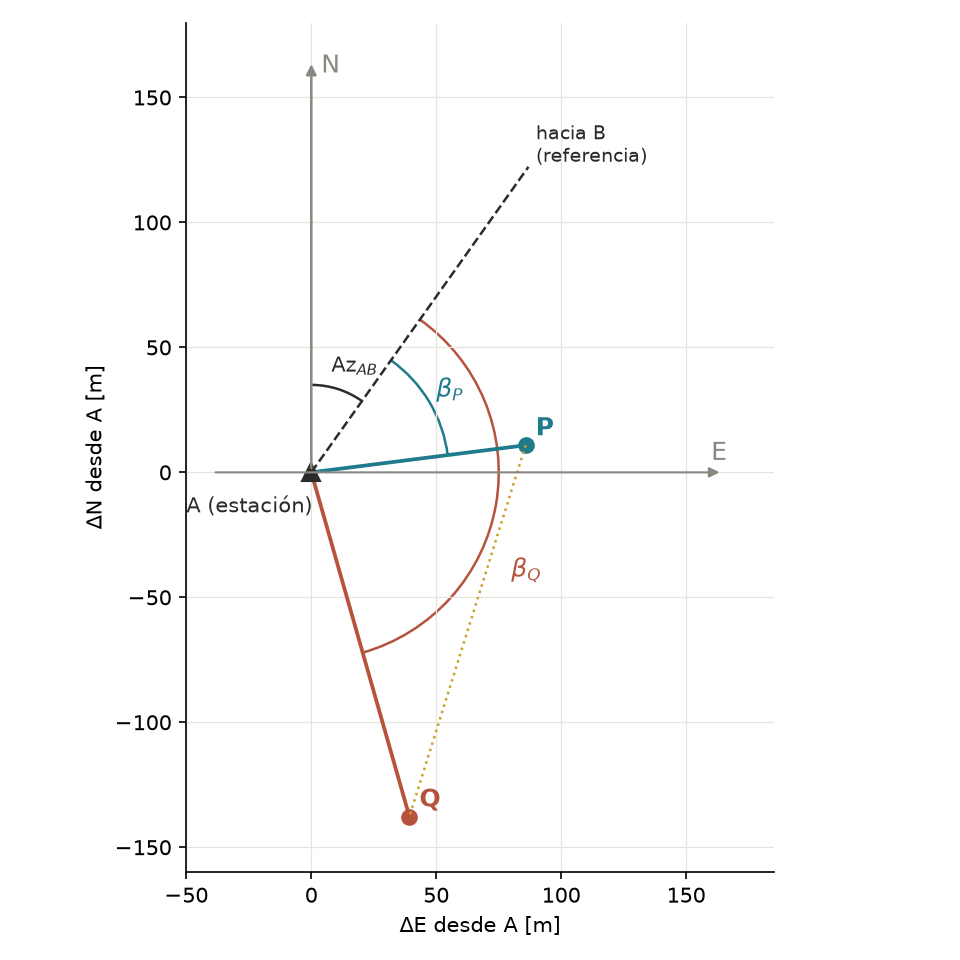
\includegraphics[width=.62\linewidth]{figuras/rotaciones/acimut_radiado.png}
\caption{Radiado desde la estación \(A\), en metros relativos a \(A\). La visual a la
referencia \(B\) tiene acimut \(\mathrm{Az}_{AB}\approx35^\circ\,24'\); los ángulos
\(\beta_P\) y \(\beta_Q\) se cuentan desde esa visual en sentido horario y llevan a \(P\) y
\(Q\). El segmento punteado \(PQ\) se usa en la verificación. Generada con
\texttt{apunte/scripts/cap01\_acimut\_estacion\_total.py}.}
\label{fig:acimut-radiado}
\end{figure}

\paragraph{Verificación: la rotación conserva distancias.} La distancia entre los dos puntos
radiados puede calcularse de tres maneras independientes.
\begin{itemize}
  \item Desde las coordenadas finales: \(\overline{PQ}=\sqrt{(E_Q-E_P)^2+(N_Q-N_P)^2}=155{,}699\) m.
  \item En el sistema propio del instrumento, con el eje \(y'\) hacia \(B\) y el \(x'\)
  perpendicular hacia la derecha: allí \(P'=R(-\beta_P)(0,d_P)=(63{,}624;\ 58{,}531)\) y
  \(Q'=R(-\beta_Q)(0,d_Q)=(111{,}780;\ -89{,}533)\), y \(\overline{P'Q'}=155{,}699\) m. Las
  coordenadas finales son \(A+R(-\mathrm{Az}_{AB})\,P'\) y \(A+R(-\mathrm{Az}_{AB})\,Q'\): un
  movimiento rígido, que por la proposición~\ref{prop:propiedades-R} no cambia la distancia.
  \item Solo con las medidas, por la ley del coseno en el triángulo \(APQ\), cuyo ángulo en
  \(A\) es \(\gamma=\beta_Q-\beta_P=81^\circ\,18'\,23{,}0''\):
  \(\overline{PQ}=\sqrt{d_P^2+d_Q^2-2\,d_Pd_Q\cos\gamma}=155{,}699\) m.
\end{itemize}
Los tres valores coinciden (la diferencia es menor que \(10^{-9}\) m), y también se recuperan
\(\overline{AP}=86{,}452\) m y \(\overline{AQ}=143{,}217\) m desde las coordenadas. La ley del
coseno es el producto interno de la sección~\ref{sec:interno} escrito con normas y ángulo; que
dé lo mismo es la conservación del producto interno por \(R\).

\paragraph{El cuadrante importa.} Para el acimut de \(P\) hacia \(Q\) los incrementos son
\(\Delta E=-46{,}515\) m y \(\Delta N=-148{,}588\) m. El cociente \(\Delta E/\Delta N\) es
positivo y \(\arctan(\Delta E/\Delta N)=17{,}382484^\circ\), que es la dirección opuesta: con
los dos incrementos negativos el punto \(Q\) está al sur y al oeste de \(P\), en el tercer
cuadrante. La función de dos argumentos da
\[
\mathrm{Az}_{PQ}=\operatorname{atan2}(-46{,}515;\ -148{,}588)=197{,}382484^\circ=197^\circ\,22'\,56{,}9'',
\]
y el acimut inverso es \(\mathrm{Az}_{QP}=17^\circ\,22'\,56{,}9''\). El valor ingenuo coincidía
con \(\mathrm{Az}_{QP}\): el error es exactamente media vuelta.

\unidadInteractiva{01a_punto_quieto}{Rotaciones I: el punto no se movió}{Explorá: girá los ejes un ángulo como el de orientación \(\mathrm{Az}_{AB}\) y comprobá que el punto queda quieto aunque cambien sus coordenadas, como pasa al llevar \(P'\) del sistema del instrumento al de la faja.}

\unidadInteractiva{02_producto_interno}{Producto interno: proyección, longitud, ángulo}{Verificá: con dos vectores de longitudes \(d_P\) y \(d_Q\) que formen el ángulo \(\gamma\), comprobá que la distancia entre sus extremos es la que da la ley del coseno.}

\section{En profundidad}

El apéndice~\ref{ap:infinitesimales} desarrolla las rotaciones infinitesimales y su relación
con la exponencial; el apéndice~\ref{ap:rot3d} construye las matrices de rotación 3D y la
fórmula de Rodrigues para un eje arbitrario.

\subsection{Rotaciones pequeñas}

\begin{definicion}[Generadores infinitesimales]
Los \emph{generadores} de las rotaciones elementales son las derivadas en \(\theta=0\):
\[
A_x=\left.\frac{dR_x}{d\theta}\right|_{0}=
\begin{pmatrix}0&0&0\\0&0&-1\\0&1&0\end{pmatrix},\quad
A_y=\left.\frac{dR_y}{d\theta}\right|_{0}=
\begin{pmatrix}0&0&1\\0&0&0\\-1&0&0\end{pmatrix},\quad
A_z=\left.\frac{dR_z}{d\theta}\right|_{0}=
\begin{pmatrix}0&-1&0\\1&0&0\\0&0&0\end{pmatrix}.
\]
\end{definicion}

\begin{proposicion}\label{prop:rot-pequenas}
Para un ángulo pequeño \(\varepsilon\),
\(R_x(\varepsilon)=I+\varepsilon A_x+O(\varepsilon^2)\), y lo mismo para \(y\) y \(z\).
Además, los dos órdenes de composición coinciden a primer orden y difieren a segundo orden en
\[
(I+\varepsilon A_x)(I+\varepsilon A_y)-(I+\varepsilon A_y)(I+\varepsilon A_x)
=\varepsilon^2(A_xA_y-A_yA_x)=\varepsilon^2A_z.
\]
\end{proposicion}

\begin{demostracion}
La primera afirmación es el desarrollo de Taylor de \(\cos\varepsilon=1+O(\varepsilon^2)\) y
\(\sin\varepsilon=\varepsilon+O(\varepsilon^3)\) en cada entrada (detalle en el
apéndice~\ref{ap:infinitesimales}). Al desarrollar los productos,
\((I+\varepsilon A_x)(I+\varepsilon A_y)=I+\varepsilon(A_x+A_y)+\varepsilon^2A_xA_y\), y el
orden inverso cambia solo el término \(\varepsilon^2A_yA_x\). Multiplicando las matrices,
\(A_xA_y\) tiene un único \(1\) en la posición \((2,1)\) y \(A_yA_x\) un único \(1\) en la
posición \((1,2)\); su diferencia es \(A_z\).
\end{demostracion}

\begin{ejemplo}[Cuánto no conmutan dos giros de \(0{,}01\) rad]
Con \(\varepsilon=0{,}01\), el cálculo exacto da
\(R_x(\varepsilon)R_y(\varepsilon)-R_y(\varepsilon)R_x(\varepsilon)\approx\varepsilon^2A_z\),
cuyas entradas no nulas son \(\mp0{,}0001\): cien veces menores que el giro mismo. Por eso las
rotaciones muy pequeñas parecen conmutar, aunque no conmutan exactamente; y la diferencia es,
ella misma, un giro pequeño alrededor del tercer eje.
\end{ejemplo}

\subsection{Eje de rotación, autovectores y exponencial}\label{sec:eje-exp}

\subsubsection{El eje como dirección fija}

\begin{definicion}[Rotación propia y eje]
Una matriz \(R\) de \(3\times3\) es una \emph{rotación propia} si \(R^TR=I\) y \(\det R=1\).
Un \emph{eje} de \(R\) es una dirección \(v\neq0\) con \(Rv=v\); en el lenguaje del
capítulo~\ref{cap:autovectores}, un autovector de autovalor \(1\).
\end{definicion}

\begin{teorema}[Euler]\label{teo:euler-eje}
Toda rotación propia de \(\R^3\) tiene un eje.
\end{teorema}

\begin{demostracion}
Hay que ver que \((R-I)v=0\) tiene solución no nula, es decir, que \(\det(R-I)=0\). Usando
\(R^TR=I\) y \(\det R=\det R^T=1\):
\[
\det(R-I)=\det\bigl(R^T(R-I)\bigr)=\det(I-R^T)=\det\bigl((I-R)^T\bigr)=\det(I-R)
=(-1)^3\det(R-I).
\]
Un número igual a su opuesto es cero.
\end{demostracion}

Para hallar el ángulo alcanza la traza: en una base ortonormal cuyo tercer vector es el eje,
\(R\) tiene un bloque \(R(\theta)\) de \(2\times2\) y un \(1\) en la diagonal, de modo que
\(\operatorname{tr}R=1+2\cos\theta\) (la traza no depende de la base;
sección~\ref{sec:cambio-base}).

\begin{ejemplo}[Eje y ángulo de una permutación de ejes]\label{ej:permutacion}
La matriz
\[
P=\begin{pmatrix}0&0&1\\1&0&0\\0&1&0\end{pmatrix}
\]
tiene columnas \(Pe_x=e_y\), \(Pe_y=e_z\), \(Pe_z=e_x\): permuta cíclicamente los ejes. Es
ortogonal con \(\det P=1\). El sistema \((P-I)v=0\) da \(v_3=v_1\), \(v_1=v_2\), \(v_2=v_3\):
el eje es \((1,1,1)\). La traza es \(0=1+2\cos\theta\), de modo que \(\cos\theta=-1/2\) y
\(\theta=120^\circ\).
\end{ejemplo}

\subsubsection{Exponencial de matrices}

\begin{definicion}[Exponencial de una matriz]
La exponencial de una matriz cuadrada \(A\) es la serie
\[
  e^A=I+A+\frac{A^2}{2!}+\frac{A^3}{3!}+\cdots,
\]
que converge para toda \(A\) (la norma del término \(k\)-ésimo está acotada por
\(\|A\|^k/k!\)). Un \emph{logaritmo} de \(R\) es una matriz \(A\) con \(e^A=R\).
\end{definicion}

Si \(R=e^A\), la familia \(e^{\tau A}\), \(0\le\tau\le1\), describe una trayectoria continua
desde la identidad hasta \(R\), y \(e^{A/n}\) es un paso pequeño que, aplicado \(n\) veces,
produce \(e^A\).

\begin{ejemplo}[La rotación plana como exponencial]
Sea \(J=\left(\begin{smallmatrix}0&-1\\1&0\end{smallmatrix}\right)\). Como \(J^2=-I\), las potencias pares de
\(\tau J\) son \(\pm\tau^{2m}I\) y las impares \(\pm\tau^{2m+1}J\); agrupando,
\[
e^{\tau J}=\Bigl(1-\frac{\tau^2}{2!}+\cdots\Bigr)I+\Bigl(\tau-\frac{\tau^3}{3!}+\cdots\Bigr)J
=\cos\tau\,I+\sin\tau\,J=R(\tau).
\]
Para \(\tau=\pi/6\) la serie sumada numéricamente da las entradas \(0{,}866\) y \(0{,}500\) de
\(R(30^\circ)\). El generador \(J\) es el análogo plano de \(A_z\).
\end{ejemplo}

\begin{proposicion}[Generador antisimétrico]\label{prop:generador}
Sea \(R\) la rotación de ángulo \(\theta\in[0,\pi)\) alrededor del eje unitario \(u\). Entonces
\(R=e^{A}\) con
\[
A=
\begin{pmatrix}
0&-\omega_z&\omega_y\\
\omega_z&0&-\omega_x\\
-\omega_y&\omega_x&0
\end{pmatrix},
\qquad \omega=(\omega_x,\omega_y,\omega_z)=\theta\,u,
\]
y es el único logaritmo antisimétrico con \(|\omega|<\pi\) (el \emph{logaritmo principal}).
El vector \(\omega\) indica el eje y su norma es el ángulo.
\end{proposicion}

La demostración combina la fórmula de Rodrigues del apéndice~\ref{ap:rot3d} con la relación
entre generadores y exponencial del apéndice~\ref{ap:infinitesimales}. Numéricamente, el
logaritmo se calcula con \texttt{scipy.linalg.logm}.

\begin{ejemplo}[Generador de la permutación \(P\)]
Para la matriz \(P\) del ejemplo~\ref{ej:permutacion}, \(\theta=2\pi/3\approx2{,}094\) y
\(u=(1,1,1)/\sqrt3\), de modo que
\(\omega=\tfrac{2\pi}{3\sqrt3}(1,1,1)\approx(1{,}209;\,1{,}209;\,1{,}209)\) y
\(|\omega|\approx2{,}094\) rad \(=120^\circ\).
\end{ejemplo}

\subsection{Experimento: muchos giros pequeños alrededor de los tres ejes}

Componemos muchas veces un mismo paso formado por tres giros pequeños e iguales,
\[
Q_\varepsilon
=R_z(\varepsilon)R_y(\varepsilon)R_x(\varepsilon),
\qquad \varepsilon=0{,}01,
\]
con \texttt{MMULT} en una planilla o con \texttt{numpy}. Por la
proposición~\ref{prop:rot-pequenas}, a primer orden
\(Q_\varepsilon\approx I+\varepsilon(A_x+A_y+A_z)\). La matriz \(A_x+A_y+A_z\) es la de la
proposición~\ref{prop:generador} con \(\omega=(1,1,1)\), cuya norma es \(\sqrt3\): cada paso
es, aproximadamente, un giro de \(\varepsilon\sqrt3\) alrededor de \((1,1,1)\). Después de
\(n\) pasos el ángulo acumulado es
\[
  \Theta\approx n\varepsilon\sqrt3.
\]
Para llegar a la permutación \(P\) del ejemplo~\ref{ej:permutacion} hace falta
\(\Theta=2\pi/3\), es decir \(n\approx(2\pi/3)/(0{,}01\sqrt3)\approx120{,}9\); el entero más
cercano es \(n=121\):
\[
  \Theta\approx121\cdot0{,}01\cdot\sqrt3
  \approx2{,}096\ \text{rad}
  \approx120{,}079^\circ.
\]
El producto exacto \(Q_\varepsilon^{121}\), calculado numéricamente, tiene eje
\(\approx(0{,}575;\,0{,}581;\,0{,}575)\), muy cerca de \((1,1,1)/\sqrt3\),
de componentes \(\approx0{,}577\), y ángulo \(\approx119{,}879^\circ\); sus entradas difieren de las de \(P\) en
menos de \(0{,}008\). La pequeña discrepancia es el término de segundo orden de la
proposición~\ref{prop:rot-pequenas}, acumulado a lo largo de los 121 pasos.

\subsection{Producto interno: incidencia}\label{sec:interno}

\unidadInteractiva{02_producto_interno}{Producto interno: proyección, longitud, ángulo}{Verificá: variá el ángulo \(\theta\) entre \(u\) y \(v\) y comprobá que el producto interno se anula cuando son perpendiculares.}

El producto interno sirve para proyectar y para decidir si dos vectores son ortogonales
(\(u\cdot v=0\)). En coordenadas homogéneas aparece un tercer uso.
Un punto se representa por una terna \(p=(x,y,w)^T\) y una recta \(ax+by+c=0\) por otra
terna \(\ell=(a,b,c)^T\). Son objetos distintos (se los suele dibujar con símbolos
distintos), pero ambos son vectores de \(\R^3\), y
\[
  \boxed{\ \ell\cdot p=ax+by+cw=0\quad\Longleftrightarrow\quad p\ \text{está en}\ \ell\ }.
\]
La ecuación cartesiana de la recta dice \enquote{el producto interno con la normal es
cero}. Ni \(\ell\) ni \(p\) cambian de significado si se los multiplica por un número, y la
condición tampoco.

\section{Ejercicios con solución}

\begin{ejercicio}
Calculá la imagen de \(p=(5,2)\) por la rotación de \(60^\circ\) alrededor de \(c=(2,-1)\) y
verificá que \(|p'-c|=|p-c|\).
\solucion{\(p-c=(3,3)\), \(R(60^\circ)(3,3)\approx(-1{,}098;\,4{,}098)\),
\(p'\approx(0{,}902;\,3{,}098)\); ambas distancias valen \(3\sqrt2\approx4{,}243\).}
\end{ejercicio}

\begin{ejercicio}
La matriz homogénea
\[
H=\begin{pmatrix}0&-1&4\\1&0&2\\0&0&1\end{pmatrix}
\]
representa una rotación. Hallá su
ángulo y su centro.
\solucion{La parte lineal es \(R(90^\circ)\). El centro resuelve
\((I-R)c=(4,2)\); con \(c=(x,y)\): \(x+y=4\), \(-x+y=2\), de donde \(c=(1,3)\); en efecto
\(H(1,3,1)^T=(1,3,1)^T\).}
\end{ejercicio}

\begin{ejercicio}
Un punto está a \(100\) m de una estación, en \(p=(100,0)\). Compará su rotación exacta en
\(\varepsilon=0{,}02\) rad con la aproximación \((I+\varepsilon J)p\),
\(J=\left(\begin{smallmatrix}0&-1\\1&0\end{smallmatrix}\right)\).
\solucion{Exacta \(\approx(99{,}980;\,2{,}000)\), aproximada \((100;\,2)\); el error es
\(\approx0{,}020\) m \(\approx\varepsilon^2\cdot100/2\), de segundo orden.}
\end{ejercicio}

\begin{ejercicio}
Calculá \(R_z(90^\circ)R_x(90^\circ)e_y\) y \(R_x(90^\circ)R_z(90^\circ)e_y\). ¿Conmutan?
\solucion{El primero da \(e_z\) (\(R_x\) lleva \(e_y\) a \(e_z\), que \(R_z\) deja fijo); el
segundo da \(-e_x\) (\(R_z\) lleva \(e_y\) a \(-e_x\), que \(R_x\) deja fijo). No conmutan.}
\end{ejercicio}

\begin{ejercicio}
Convertí el acimut \(\mathrm{Az}=230^\circ\) en ángulo matemático \(\theta\), y el ángulo
\(\theta=30^\circ\) en acimut.
\solucion{\(\theta=90^\circ-230^\circ=-140^\circ\equiv220^\circ\);
\(\mathrm{Az}=90^\circ-30^\circ=60^\circ\).}
\end{ejercicio}

% Traslaciones y movimientos rígidos (partición por clase: apunte/scripts/reorganizar_por_clase.py)
\chapter{Traslaciones y movimientos rígidos}\label{cap:traslaciones}

\section{La idea}

\subsection{Componer transformaciones con centros distintos}\label{sec:componer-centros}

Supongamos que giramos una figura \(90^\circ\) alrededor de un punto \(c_1\) y después
\(90^\circ\) alrededor de otro punto \(c_2\). Cada etapa es una rotación, pero ninguno de los
dos centros queda fijo en el resultado: \(c_1\) no se mueve en la primera etapa pero sí en la
segunda, y \(c_2\) se mueve en la primera. La pregunta natural es si el resultado sigue siendo
una rotación y, en ese caso, dónde está su centro.

La respuesta (proposición de la sección~\ref{sec:composicion-rotaciones}) es que los ángulos
se suman y que aparece un centro nuevo, distinto de los dos originales; en el ejemplo, una
rotación de \(180^\circ\). Solo cuando los ángulos se cancelan el resultado es una traslación,
que no tiene punto fijo.

Si una de las dos etapas es una homotecia \(\homot{c_2}{k}\) en lugar de una rotación, la parte
lineal resulta \(kR(\theta)\) y la composición es una similaridad, que también tiene un único
punto fijo cuando \(k\neq1\) (capítulo~\ref{cap:afines}).

\paragraph{Movimiento discreto y trayectoria imaginada.}
Una transformación lleva cada punto directamente a su imagen. Dibujar el movimiento como
``primero un arco alrededor de \(c_1\), después otro arco alrededor de \(c_2\)'' es una
interpolación útil para seguir las dos etapas, pero no forma parte de la transformación
compuesta: el arco único alrededor del centro nuevo une los mismos extremos por otro camino.

\begin{idea}[Idea]
Aplicar giros sucesivos a un punto lo hace recorrer arcos de circunferencia, y eso es
inevitable: la composición tiene un punto fijo, y alrededor de él todo se mueve en
círculos. Encontrar el punto fijo es entender la transformación.
\end{idea}

\section{Construcciones, cuentas y ejemplos}

\subsection{Composición de dos rotaciones de centros distintos}\label{sec:composicion-rotaciones}

La herramienta para componer rotaciones son las reflexiones: cada rotación se descompone en
dos reflexiones, y una reflexión aplicada dos veces se cancela.

\begin{definicion}[Reflexión respecto de una recta]
Sea \(L\) una recta que pasa por el punto \(q\) con ángulo de dirección \(\delta\). La
\emph{reflexión respecto de \(L\)} es la transformación \(\sigma_L\) que deja fijos los puntos
de \(L\) y lleva cada punto a su simétrico respecto de \(L\). En fórmulas,
\[
\sigma_L(p)=q+S(\delta)(p-q),\qquad
S(\delta)=\begin{pmatrix}\cos2\delta&\sin2\delta\\ \sin2\delta&-\cos2\delta\end{pmatrix}.
\]
\end{definicion}

La matriz \(S(\delta)\) deja fija la dirección \((\cos\delta,\sin\delta)\) de \(L\) y cambia
de signo la perpendicular; tiene \(\det S(\delta)=-1\), invierte la orientación y cumple
\(S(\delta)^2=I\), es decir, \(\sigma_L\circ\sigma_L\) es la identidad.

\begin{proposicion}[Dos reflexiones]\label{prop:dos-reflexiones}
Sean \(L_1\) y \(L_2\) rectas con ángulos de dirección \(\delta_1\) y \(\delta_2\).
\begin{enumerate}
  \item Si se cortan en un punto \(q\), entonces
  \(\sigma_{L_2}\circ\sigma_{L_1}=\rhoP{q,\,2(\delta_2-\delta_1)}\).
  \item Si son paralelas, \(\sigma_{L_2}\circ\sigma_{L_1}\) es una traslación.
\end{enumerate}
\end{proposicion}

\begin{demostracion}
Multiplicando y usando las fórmulas de suma,
\[
S(\delta_2)S(\delta_1)=
\begin{pmatrix}
\cos(2\delta_2-2\delta_1)&-\sin(2\delta_2-2\delta_1)\\
\sin(2\delta_2-2\delta_1)&\cos(2\delta_2-2\delta_1)
\end{pmatrix}
=R\bigl(2(\delta_2-\delta_1)\bigr).
\]
Si ambas rectas pasan por \(q\), podemos usar \(q\) como punto de las dos fórmulas:
\(\sigma_{L_2}(\sigma_{L_1}(p))=q+S(\delta_2)S(\delta_1)(p-q)=q+R(2(\delta_2-\delta_1))(p-q)\).
Si son paralelas, \(\delta_2=\delta_1\) (módulo \(\pi\)), la parte lineal de la composición es
\(R(0)=I\), y una afinidad con parte lineal \(I\) es una traslación.
\end{demostracion}

\begin{proposicion}[Composición de dos rotaciones]\label{prop:composicion-rotaciones}
Sean \(c_1\neq c_2\) y \(\alpha,\beta\) ángulos. Entonces:
\begin{enumerate}
  \item si \(\alpha+\beta\not\equiv0\pmod{2\pi}\), la composición
  \(\rhoP{c_2,\beta}\circ\rhoP{c_1,\alpha}\) es una rotación de ángulo \(\alpha+\beta\)
  alrededor de un centro \(c\);
  \item si \(\alpha+\beta\equiv0\pmod{2\pi}\), la composición es una traslación.
\end{enumerate}
El centro \(c\) se construye así: sea \(L\) la recta que une \(c_1\) con \(c_2\); sea \(M_1\)
la recta por \(c_1\) que forma con \(L\) un ángulo \(\alpha/2\) en sentido horario, y \(M_2\)
la recta por \(c_2\) que forma con \(L\) un ángulo \(\beta/2\) en sentido antihorario.
Entonces \(c=M_1\cap M_2\).
\end{proposicion}

\begin{demostracion}
Sea \(\delta_0\) el ángulo de dirección de \(L\). Entonces \(M_1\) tiene dirección
\(\delta_0-\alpha/2\) y \(M_2\), dirección \(\delta_0+\beta/2\). Por la
proposición~\ref{prop:dos-reflexiones}, como \(L\) y \(M_1\) se cortan en \(c_1\),
\[
\sigma_L\circ\sigma_{M_1}=\rhoP{c_1,\,2(\delta_0-(\delta_0-\alpha/2))}=\rhoP{c_1,\alpha},
\]
y como \(M_2\) y \(L\) se cortan en \(c_2\),
\(\sigma_{M_2}\circ\sigma_L=\rhoP{c_2,\,2(\beta/2)}=\rhoP{c_2,\beta}\). Luego
\[
\rhoP{c_2,\beta}\circ\rhoP{c_1,\alpha}
=\sigma_{M_2}\circ\sigma_L\circ\sigma_L\circ\sigma_{M_1}
=\sigma_{M_2}\circ\sigma_{M_1},
\]
porque \(\sigma_L\circ\sigma_L\) es la identidad. La diferencia de direcciones entre \(M_2\) y
\(M_1\) es \((\alpha+\beta)/2\). Si \(\alpha+\beta\not\equiv0\pmod{2\pi}\), entonces
\((\alpha+\beta)/2\not\equiv0\pmod{\pi}\), las rectas no son paralelas, se cortan en un punto
\(c\) y, otra vez por la proposición~\ref{prop:dos-reflexiones}, la composición es
\(\rhoP{c,\,\alpha+\beta}\). Si \(\alpha+\beta\equiv0\pmod{2\pi}\), las rectas \(M_1\) y
\(M_2\) son paralelas y la composición es una traslación.
\end{demostracion}

\begin{center}
\begin{tikzpicture}[scale=.95]
  \draw[muted,dotted] (-1.5,0)--(0,0);
  \draw[mainline] (-1.2,0)--(5.4,0) node[right] {$L$};
  \draw[teal,line width=.9pt] (-1.2,1.2)--(3.3,-3.3) node[below] {$M_1$};
  \draw[rust,line width=.9pt] (5.2,1.2)--(0.7,-3.3) node[below] {$M_2$};
  \fill[ink] (0,0) circle (2.4pt) node[below left] {$c_1=(0,0)$};
  \fill[ink] (4,0) circle (2.4pt) node[above left] {$c_2=(4,0)$};
  \fill[gold] (2,-2) circle (2.6pt);
  \node[labelback,text=ink] at (2,-2.55) {$c=(2,-2)$};
  \draw[teal,line width=.8pt] (.9,0) arc[start angle=0,end angle=-45,radius=.9];
  \node[text=teal,font=\small] at (1.35,-.32) {$\alpha/2$};
  \draw[rust,line width=.8pt] (3.1,0) arc[start angle=180,end angle=225,radius=.9];
  \node[text=rust,font=\small] at (2.65,-.32) {$\beta/2$};
  \draw[gold,line width=.8pt] ($(2,-2)+(45:.55)$) arc[start angle=45,end angle=135,radius=.55];
  \node[text=gold!80!ink,font=\small] at (2,-1.15) {$\tfrac{\alpha+\beta}{2}$};
\end{tikzpicture}
\end{center}

\begin{ejemplo}[Dos cuartos de vuelta con centros distintos]\label{ej:composicion-centros}
Sean \(c_1=(0,0)\), \(\alpha=90^\circ\), \(c_2=(4,0)\), \(\beta=90^\circ\). Como
\(\alpha+\beta=180^\circ\not\equiv0\), la proposición anuncia una rotación de \(180^\circ\).

\emph{Construcción.} \(L\) es el eje \(x\). \(M_1\) pasa por \((0,0)\) con dirección
\(-45^\circ\): es la recta \(y=-x\). \(M_2\) pasa por \((4,0)\) con dirección \(45^\circ\):
es \(y=x-4\). Igualando, \(-x=x-4\), de donde \(x=2\), \(y=-2\): el centro es \(c=(2,-2)\).

\emph{Cuenta matricial.} Con \(R(90^\circ)\) del ejemplo de la sección~\ref{sec:rot-plano}, la
traslación de la segunda rotación es \((I-R(90^\circ))c_2=(4,0)-(0,4)=(4,-4)\), y en
coordenadas homogéneas
\[
H_2H_1=
\begin{pmatrix}0&-1&4\\1&0&-4\\0&0&1\end{pmatrix}
\begin{pmatrix}0&-1&0\\1&0&0\\0&0&1\end{pmatrix}
=\begin{pmatrix}-1&0&4\\0&-1&-4\\0&0&1\end{pmatrix}.
\]
La parte lineal es \(-I=R(180^\circ)\). El punto fijo resuelve \(-c+(4,-4)=c\), o sea
\(c=(2,-2)\), el mismo que dio la construcción. La composición es
\(\rhoP{(2,-2),\,180^\circ}\), es decir \(p\mapsto(4,-4)-p\).
\end{ejemplo}

\subsubsection{Experimento: rotar una figura con dos centros distintos}

Tomemos el triángulo de vértices \((1,1)\), \((3,1)\), \((1,2)\) y apliquemos las dos
rotaciones del ejemplo~\ref{ej:composicion-centros}. Tras \(\rhoP{c_1,90^\circ}\) los vértices
van a \((-1,1)\), \((-1,3)\), \((-2,1)\); tras \(\rhoP{c_2,90^\circ}\), a \((3,-5)\),
\((1,-5)\), \((3,-6)\). La rotación única \(\rhoP{(2,-2),180^\circ}\), \(p\mapsto(4,-4)-p\),
da exactamente los mismos tres puntos: por ejemplo \((4,-4)-(1,1)=(3,-5)\).

\begin{center}
\begin{tikzpicture}[scale=.62]
  \draw[axisline,-{Latex[length=2mm]}] (-2.8,0)--(5.4,0) node[right] {$x$};
  \draw[axisline,-{Latex[length=2mm]}] (0,-6.6)--(0,3.6) node[above] {$y$};
  \draw[teal,line width=1.1pt,fill=teal!15] (1,1)--(3,1)--(1,2)--cycle;
  \draw[gold,line width=1.1pt,fill=gold!15] (-1,1)--(-1,3)--(-2,1)--cycle;
  \draw[rust,line width=1.1pt,fill=rust!15] (3,-5)--(1,-5)--(3,-6)--cycle;
  \draw[auxline,-{Latex[length=2mm]}] (1,1) arc[start angle=45,end angle=135,radius=1.414];
  \draw[auxline,-{Latex[length=2mm]}] (-1,1) arc[start angle=168.69,end angle=258.69,radius=5.099];
  \fill[ink] (0,0) circle (2.2pt) node[below left] {$c_1$};
  \fill[ink] (4,0) circle (2.2pt) node[above] {$c_2$};
  \fill[ink] (2,-2) circle (2.4pt) node[right] {$c=(2,-2)$};
  \node[labelback,text=teal,font=\small] at (3.3,1.8) {original};
  \node[labelback,text=gold!80!ink,font=\small,anchor=east] at (-2.3,2.4) {tras \(\rhoP{c_1,90^\circ}\)};
  \node[labelback,text=rust,font=\small] at (3.9,-6.2) {final};
\end{tikzpicture}
\end{center}

El vértice \((1,1)\) recorre primero un arco alrededor de \(c_1\) y después otro alrededor de
\(c_2\); el resultado final, en cambio, es un único medio giro alrededor de \(c=(2,-2)\), un
punto que no aparece en ninguna de las dos etapas.

\section{En profundidad}

\section{Ejercicios propuestos}

\begin{ejercicio}
Calcular \(\rhoP{(2,0),-90^\circ}\circ\rhoP{(0,0),90^\circ}\) y explicar el resultado con la
proposición~\ref{prop:composicion-rotaciones}.
\solucion{Como \(90^\circ+(-90^\circ)=0\), es una traslación: la matriz homogénea es
\(\left(\begin{smallmatrix}1&0&2\\0&1&2\\0&0&1\end{smallmatrix}\right)\), traslación de vector \((2,2)\).}
\end{ejercicio}

% De las reflexiones a las afinidades y las coordenadas homogéneas (partición por clase: apunte/scripts/reorganizar_por_clase.py)
\chapter{De las reflexiones a las afinidades y las coordenadas homogéneas}\label{cap:afines}\label{sec:bloque-euclideas}


\section{La idea (reflexiones y similaridades)}

Reflejamos y escalamos. Con reflexiones se construyen rotaciones, y con una escala común se pasa a las similaridades. Seguimos el hilo de las clases dictadas, con los resúmenes del profesor como guía.

\subsection{Reflejar y componer}\label{sec:reflejar}

{\small\vspace{1mm}\linkUnidad{03_reflexiones_similaridades}{Simulación interactiva: Unidad 5 — Reflexiones y similaridades}\par}


Una reflexión invierte una figura respecto de un centro o de una recta. Aplicada dos veces
respecto del mismo elemento devuelve la figura original. Esta propiedad se llama involución.

La riqueza geométrica aparece al combinar reflexiones distintas:
\begin{itemize}
  \item dos reflexiones puntuales producen una traslación;
  \item dos reflexiones en rectas paralelas producen una traslación perpendicular a ellas;
  \item dos reflexiones en rectas secantes producen una rotación alrededor de su intersección;
  \item tres reflexiones puntuales vuelven a producir una reflexión puntual y construyen un
  paralelogramo.
\end{itemize}

\paragraph{Primera traducción algebraica.}
\[
  \rho_b(x)=2b-x.
\]
La diferencia \(\rho_b(x)-b=-(x-b)\) indica que la imagen conserva la distancia a \(b\),
pero queda en la dirección opuesta. Al componer dos reflexiones, los términos que dependen de
\(x\) recuperan su signo y queda un desplazamiento constante.

\begin{idea}[Qué debe observarse]
Cada reflexión individual cambia la orientación. Dos reflexiones vuelven a preservarla. La
posición relativa de los centros o de los ejes decide si el resultado se interpreta como
traslación o como rotación.
\end{idea}

\begin{idea}[En palabras del profesor]
``Vimos que con reflexiones podíamos construir rotaciones (con un argumento coloquial
sobre que un par de reflexiones sucesivas no altera las distancias, pero tiene un punto
fijo, así que tiene que ser una rotación)'' (resumen de clase 3, cursada 2025).
\end{idea}

\subsection{Escalar: homotecias y similaridades}\label{sec:escalar}

Una homotecia cambia el tamaño respecto de un centro. Cada punto permanece sobre la recta que
lo une con ese centro. Si la razón es positiva conserva el semirayo; si es negativa pasa al
semirayo opuesto.

Una similaridad combina escala uniforme, giro y, eventualmente, reflexión o traslación. La
figura puede cambiar de tamaño y posición, pero conserva sus ángulos y sus proporciones. Dos
triángulos relacionados por una similaridad tienen la misma forma.

\paragraph{Primera traducción algebraica.}
\[
  x'=o+k(x-o).
\]
El término \(x-o\) mira el punto desde el centro. Multiplicarlo por \(k\) cambia su distancia
y, si \(k<0\), también invierte el semirayo.

\begin{idea}[En palabras del profesor]
``Así como la rotación se expresa en complejos también se expresa la escala, que en
matrices se representa con una matriz múltiplo de la identidad'' (resumen de clase 1, cursada 2025).
\end{idea}

\section{Construcciones, cuentas y ejemplos (reflexiones y similaridades)}

Este nivel es la guía de transformaciones. Reproducimos los enunciados de \texttt{Ejercicios.pdf}, material docente enviado por la cátedra, y resolvemos cada definición y cada teorema de dos maneras, con una construcción y con un ejemplo con vectores. La resolución es desarrollo nuestro.

{\small\vspace{1mm}\linkUnidad{03_reflexiones_similaridades}{Simulación interactiva: Unidad 5 — Reflexiones y similaridades}\par}

\subsection{Enunciados originales de la guía}

Los textos siguientes reproducen los enunciados de \texttt{Ejercicios.pdf}. Se normalizaron
únicamente los cortes de línea, la notación matemática y errores tipográficos evidentes; las
dos páginas originales se incluyen completas como anexo facsimilar al final del documento.

\begin{enunciado}[Definición 1]
La reflexión del punto \(a\) por un punto \(b\) es la operación que lleva el punto \(a\) al
punto que está sobre la recta \(\overline{ab}\), a la misma distancia de \(b\) que \(a\),
pero al otro lado de \(b\). Se llama \(\rho_b(a)\).
\end{enunciado}

\begin{enunciado}[Teorema 1]
\(\rho_a\rho_b\), la composición de dos reflexiones, es una traslación. Puede ser expresada
algebraicamente con la suma de un vector constante o geométricamente como el desplazamiento
según un segmento fijo.
\end{enunciado}

\begin{enunciado}[Teorema 2]
Si \(\rho_d=\rho_a\rho_b\rho_c\), entonces el polígono \(abcda\) es un paralelogramo.
\end{enunciado}

\begin{enunciado}[Observación]
Con esta operación puede definirse la suma y resta de vectores. ¿De qué modo? ¿Cómo se
relaciona esto con la propiedad de que sea inversiva la transformación, es decir, que al
aplicarla dos veces se anula?
\end{enunciado}

\begin{enunciado}[Definición 2]
La reflexión del punto \(a\) por la recta \(B\), \(\varphi_B(a)\), es la operación que lleva
el punto \(a\) al punto que está sobre la perpendicular a \(B\) que pasa por \(a\), a la misma
distancia que \(a\) de \(B\), pero al otro lado de la recta \(B\).
\end{enunciado}

\begin{enunciado}[Teorema 3]
Si \(\Theta_{AB}=\varphi_A\varphi_B\) y \(A\) es paralela a \(B\), entonces
\(\Theta_{AB}\) es una traslación. Puede ser expresada algebraicamente con la suma de un
vector constante o geométricamente como el desplazamiento según un segmento fijo.
\end{enunciado}

\begin{enunciado}[Teorema 4]
Si \(\Theta_{AB}=\varphi_A\varphi_B\) y \(A\) no es paralela a \(B\), entonces
\(\Theta_{AB}\) es una rotación.
\end{enunciado}

\begin{enunciado}[Teorema 5]
Si \(\Theta_{ABCD}=\Theta_{AB}\Theta_{CD}\), con \(\Theta_{AB}\) una traslación y
\(\Theta_{CD}\) una rotación, entonces \(\Theta_{ABCD}\) es una rotación. Además,
\(\Theta_{CDAB}=\Theta_{CD}\Theta_{AB}\) es también una rotación, pero es distinta.
\end{enunciado}

\begin{enunciado}[Definición 3]
Una homotecia con centro en el punto \(o\) y razón \(k\), nombrada \(\eta_o^k\), lleva un
punto \(a\) a otro sobre la recta \(\overline{oa}\), de forma que
\[
  \frac{d\bigl(o,\eta_o^k(a)\bigr)}{d(o,a)}=k,
\]
donde \(d(a,b)\) es la distancia entre el punto \(a\) y el punto \(b\). Los puntos \(a\) y
\(\eta_o^k(a)\) están al mismo lado del punto \(o\) en la recta \(\overline{oa}\).
\end{enunciado}

\begin{atencion}[Precisión sobre el texto original]
La razón entre distancias es siempre no negativa. Por eso, la redacción original corresponde
al caso \(k>0\). Para una razón firmada debe escribirse
\[
\eta_o^k(a)=o+k(a-o),
\qquad
\frac{d\bigl(o,\eta_o^k(a)\bigr)}{d(o,a)}=|k|.
\]
Punto e imagen están del mismo lado de \(o\) si \(k>0\), y en lados opuestos si \(k<0\).
\end{atencion}

\begin{enunciado}[Teorema 6]
Cualquier transformación de similaridad del plano puede expresarse como la composición
\(\varphi_A\varphi_B\eta_o^k\), donde el punto \(o\) es la intersección de las rectas
\(A\) y \(B\), y es el punto fijo de la transformación. Dado un triángulo y su imagen bajo
esta transformación puede hallarse el punto \(o\) con la construcción de Euler indicada en
la guía original.
\end{enunciado}

\begin{atencion}[Alcance del Teorema 6 original]
Tal como está escrito, el enunciado es demasiado general. La composición de dos reflexiones
y una homotecia describe una similaridad directa con punto fijo. Una similaridad inversa
requiere una cantidad impar de reflexiones, y una traslación no posee punto fijo finito.
\end{atencion}

\begin{enunciado}[Ejercicios]
Para cada una de las definiciones y teoremas expuestos, verificar la conclusión con un ejemplo
gráfico y construyendo un ejemplo algebraico con vectores. Pista para las reflexiones: para
hallar la proyección perpendicular de un punto sobre una recta puede usarse el producto
interno o construir la ecuación vectorial de la perpendicular usando el vector normal que
surge de la ecuación canónica de la recta.
\end{enunciado}

\subsection{Resolución completa de la guía}

La consigna de la guía no contiene una lista de problemas independientes. Solicita verificar
\textbf{cada definición y cada teorema} de dos maneras: mediante una construcción geométrica
y mediante un ejemplo algebraico con vectores. Las secciones siguientes constituyen esa
resolución punto por punto.

\begin{center}
\begin{tabularx}{\textwidth}{>{\bfseries}p{34mm} X X}
\toprule
Ítem de la guía & Verificación geométrica & Verificación algebraica\\
\midrule
Definición 1 & punto medio y segmentos iguales & \(\rho_b(x)=2b-x\)\\
Teorema 1 & desplazamiento constante & composición de dos reflexiones puntuales\\
Teorema 2 & diagonales que se bisecan & \(d=a-b+c\)\\
Definición 2 & perpendicular y distancias iguales & proyección mediante el vector normal\\
Teorema 3 & avance perpendicular de longitud \(2h\) & composición con normales paralelos\\
Teorema 4 & ángulo final igual a \(2\theta\) & producto de matrices de reflexión\\
Teorema 5 & mismo giro, distinto centro & resolución del punto fijo\\
Definición 3 & rayos desde el centro & \(\eta_o^k(x)=o+k(x-o)\)\\
Teorema 6 & escala y giro con centro común & \(S(x)=o+\lambda R(x-o)\)\\
\bottomrule
\end{tabularx}
\end{center}

\begin{idea}[Cómo reconocer que un ítem está resuelto]
Cada apartado presenta el dibujo o construcción, la propiedad geométrica que debe observarse,
la demostración vectorial y un ejemplo numérico. Los ejercicios del final son práctica
adicional y no sustituyen estas soluciones.
\end{idea}

\subsection{Guía resuelta: reflexión respecto de un punto}

\subsubsection{Definición 1}

La reflexión de \(x\) respecto del punto \(b\) deja a \(b\) como punto medio del segmento
que une \(x\) con su imagen. Por lo tanto,
\[
  \frac{x+\rhoP{b}(x)}{2}=b
  \qquad\Longrightarrow\qquad
  \boxed{\rhoP{b}(x)=2b-x}.
\]

\begin{center}
\begin{tikzpicture}[scale=1.0]
  \coordinate (x) at (1,1.5);
  \coordinate (b) at (5,2.4);
  \coordinate (xp) at (9,3.3);
  \draw[auxline] (.4,1.36)--(9.6,3.44);
  \draw[decorate,decoration={brace,amplitude=5pt,mirror},teal]
    (x)--node[below=5pt,font=\small] {$d(x,b)$}(b);
  \draw[decorate,decoration={brace,amplitude=5pt,mirror},teal]
    (b)--node[below=5pt,font=\small] {$d(b,\rho_b(x))$}(xp);
  \fill[teal] (x) circle (2.4pt) node[above left] {$x$};
  \fill[ink] (b) circle (2.7pt) node[above] {$b$};
  \fill[rust] (xp) circle (2.4pt) node[above right] {$\rho_b(x)$};
\end{tikzpicture}
\end{center}

\begin{resultado}[Propiedades inmediatas]
\[
  \rhoP{b}\bigl(\rhoP{b}(x)\bigr)=x,
  \qquad
  \rhoP{b}(b)=b,
  \qquad
  \rhoP{b}(x)-b=-(x-b).
\]
Es una transformación involutiva: aplicarla dos veces devuelve el punto original.
\end{resultado}

\paragraph{Ejemplo.}
Si \(b=(2,1)\) y \(x=(5,3)\), entonces
\[
  \rhoP{b}(x)=2(2,1)-(5,3)=(-1,-1).
\]
El punto medio entre \((5,3)\) y \((-1,-1)\) es efectivamente \((2,1)\).

\subsection{Guía resuelta: dos reflexiones puntuales}

\subsubsection{Teorema 1: la composición es una traslación}

Sean \(a,b\in\R^2\). Aplicando primero \(\rhoP{b}\) y luego \(\rhoP{a}\):
\[
\begin{aligned}
  \rhoP{a}\rhoP{b}(x)
  &=\rhoP{a}(2b-x)\\
  &=2a-(2b-x)\\
  &=x+2(a-b).
\end{aligned}
\]

\begin{resultado}[Conclusión]
\[
  \boxed{\rhoP{a}\rhoP{b}=T_{\,2(a-b)}}
\]
La composición desplaza todos los puntos por el mismo vector \(2(a-b)\). No posee puntos
fijos salvo el caso degenerado \(a=b\), en el cual es la identidad.
\end{resultado}

\begin{center}
\begin{tikzpicture}[scale=.92]
  \coordinate (x) at (.7,1);
  \coordinate (b) at (3,1.6);
  \coordinate (y) at (5.3,2.2);
  \coordinate (a) at (6.8,2.6);
  \coordinate (z) at (8.3,3);
  \draw[auxline] (.2,.87)--(8.8,3.13);
  \draw[mainline,-{Latex[length=2.8mm]}] (x)--(z);
  \fill[teal] (x) circle (2.4pt) node[labelback,below left] {$x$};
  \fill[ink] (b) circle (2.4pt) node[labelback,above] {$b$};
  \fill[rust] (y) circle (2.4pt) node[labelback,below] {$\rho_b(x)$};
  \fill[ink] (a) circle (2.4pt) node[labelback,above] {$a$};
  \fill[teal] (z) circle (2.4pt) node[labelback,above right] {$\rho_a\rho_b(x)$};
  \node[labelback,font=\small,text=tealdark,above=16pt] at ($(x)!.5!(z)$)
    {mismo desplazamiento para cualquier \(x\)};
\end{tikzpicture}
\end{center}

\paragraph{Ejemplo.}
Con \(a=(3,2)\) y \(b=(1,1)\), la traslación resultante tiene vector
\[
  2(a-b)=2(2,1)=(4,2).
\]
Para \(x=(2,-1)\): \(\rhoP{b}(x)=(0,3)\) y
\(\rhoP{a}(0,3)=(6,1)=x+(4,2)\).

\subsection{Guía resuelta: tres reflexiones puntuales}

\subsubsection{Teorema 2: aparece un paralelogramo}

La composición de tres reflexiones puntuales vuelve a ser una reflexión puntual:
\[
\begin{aligned}
\rhoP{a}\rhoP{b}\rhoP{c}(x)
  &=2a-\bigl(2b-(2c-x)\bigr)\\
  &=2(a-b+c)-x.
\end{aligned}
\]
Si \(\rhoP{d}=\rhoP{a}\rhoP{b}\rhoP{c}\), entonces
\[
  \boxed{d=a-b+c}.
\]
Al reordenar:
\[
  a+c=b+d.
\]
Esta es precisamente la condición vectorial para que las diagonales del cuadrilátero
\(a b c d\) tengan el mismo punto medio.

\begin{center}
\begin{tikzpicture}[scale=1.0]
  \coordinate (a) at (1,1);
  \coordinate (b) at (5,1.2);
  \coordinate (c) at (7.2,4);
  \coordinate (d) at (3.2,3.8);
  \draw[mainline] (a)--(b)--(c)--(d)--cycle;
  \draw[auxline] (a)--(c);
  \draw[auxline] (b)--(d);
  \fill[teal] (a) circle (2.4pt) node[below left] {$a$};
  \fill[teal] (b) circle (2.4pt) node[below right] {$b$};
  \fill[rust] (c) circle (2.4pt) node[above right] {$c$};
  \fill[rust] (d) circle (2.4pt) node[above left] {$d=a-b+c$};
  \fill[ink] (4.1,2.5) circle (2pt);
  \node[labelback,font=\small] at (4.15,2.02) {punto medio común};
  \draw[-{Latex[length=2.2mm]},rust,line width=.8pt] (a)--(b);
  \draw[-{Latex[length=2.2mm]},rust,line width=.8pt] (d)--(c);
\end{tikzpicture}
\end{center}

\paragraph{Ejemplo.}
Si \(a=(1,1)\), \(b=(4,1)\) y \(c=(6,3)\), entonces
\[
  d=(1,1)-(4,1)+(6,3)=(3,3).
\]
Se verifica \(a+c=(7,4)=b+d\); por lo tanto, las diagonales se bisecan.

\begin{idea}[Suma y resta de vectores]
La fórmula \(d=a-b+c\) permite construir geométricamente la operación
\(a+c-b\). Elegido un origen \(b\), el punto \(d\) representa la suma de los
vectores \(\overrightarrow{ba}+\overrightarrow{bc}\).

La suma \(u+v\) se obtiene llevando ambos vectores a un origen común y completando el
paralelogramo. La resta \(u-v\) se interpreta como \(u+(-v)\), donde \(-v\) surge de reflejar
el extremo de \(v\) respecto de su origen. Esto se relaciona con la involución porque
\[
  \rho_b^2=\operatorname{Id};
\]
reflejar dos veces no ``anula'' el punto, sino que devuelve exactamente la posición inicial.
\end{idea}

\subsection{Guía resuelta: reflexión respecto de una recta}

\subsubsection{Definición 2 y fórmula con proyección}

Sea la recta
\[
  B=\{x\in\R^2:n\cdot x=c\},
\]
donde \(n\neq0\) es un vector normal. La proyección ortogonal de \(x\) sobre \(B\) es
\[
  p=x-\frac{n\cdot x-c}{\lVert n\rVert^2}\,n.
\]
Como \(p\) debe ser el punto medio entre \(x\) y su reflejo:
\[
  \boxed{\refl{B}(x)=2p-x
  =x-2\frac{n\cdot x-c}{\lVert n\rVert^2}\,n}.
\]

\begin{center}
\begin{tikzpicture}[scale=1.0]
  \coordinate (x) at (2,4.4);
  \coordinate (p) at (4.8,2.4);
  \coordinate (xp) at (7.6,.4);
  \draw[rust,line width=1.1pt] (.4,.45)--(8.8,3.95)
    node[right,font=\small] {$B$};
  \draw[auxline] (x)--(xp);
  \draw[mainline] ($(p)+(-.32,.15)$)--($(p)+(-.17,.47)$)--($(p)+(.15,.32)$);
  \fill[teal] (x) circle (2.5pt) node[above left] {$x$};
  \fill[ink] (p) circle (2.4pt) node[above right] {$p$};
  \fill[rust] (xp) circle (2.5pt) node[below right] {$\varphi_B(x)$};
  \draw[decorate,decoration={brace,amplitude=5pt},teal]
    (x)--node[left=5pt,font=\small] {$d$}(p);
  \draw[decorate,decoration={brace,amplitude=5pt},teal]
    (p)--node[left=5pt,font=\small] {$d$}(xp);
\end{tikzpicture}
\end{center}

\paragraph{Ejemplo.}
Para \(B:\ x+2y=4\), \(n=(1,2)\) y \(x_0=(4,3)\):
\[
  n\cdot x_0-c=6,\qquad \lVert n\rVert^2=5,
\]
\[
  \refl{B}(x_0)
  =(4,3)-\frac{12}{5}(1,2)
  =\left(\frac85,-\frac95\right).
\]
La proyección es
\[
  p=(4,3)-\frac65(1,2)
  =\left(\frac{14}{5},\frac35\right).
\]
Además,
\[
  x_0-p=p-\refl{B}(x_0)=\frac65(1,2),
\]
lo que verifica simultáneamente que ambos segmentos tienen la misma longitud y que son
perpendiculares a la recta, pues son paralelos al normal \(n=(1,2)\).

\subsection{Guía resuelta: reflexiones en rectas paralelas}

\subsubsection{Teorema 3: la composición es una traslación}

Tomemos rectas paralelas con un normal unitario \(n\):
\[
  A:\ n\cdot x=\alpha,
  \qquad
  B:\ n\cdot x=\beta.
\]
Sus reflexiones son
\[
  \refl{A}(x)=x-2(n\cdot x-\alpha)n,
  \qquad
  \refl{B}(x)=x-2(n\cdot x-\beta)n.
\]
Al componer:
\[
  \boxed{\refl{A}\refl{B}(x)=x+2(\alpha-\beta)n}.
\]

\begin{center}
\begin{tikzpicture}[scale=.94]
  \draw[rust,line width=1.1pt] (1,.5)--(1,5) node[above] {$B$};
  \draw[rust,line width=1.1pt] (4,.5)--(4,5) node[above] {$A$};
  \coordinate (x) at (0,1.2);
  \coordinate (y) at (2,1.2);
  \coordinate (z) at (6,1.2);
  \draw[auxline] (x)--(z);
  \draw[mainline,-{Latex[length=2.8mm]}] (x)--(z);
  \fill[teal] (x) circle (2.5pt) node[below] {$x$};
  \fill[rust] (y) circle (2.5pt) node[below] {$\varphi_B(x)$};
  \fill[teal] (z) circle (2.5pt) node[below] {$\varphi_A\varphi_B(x)$};
  \draw[<->,muted] (1,4.1)--node[above,font=\small] {$h$}(4,4.1);
  \node[font=\small,text=tealdark] at (3,2.3) {desplazamiento \(2h\)};
\end{tikzpicture}
\end{center}

\paragraph{Lectura geométrica.}
La primera reflexión cruza \(B\); la segunda cruza \(A\). El desplazamiento total es
perpendicular a ambas rectas y su módulo es dos veces la distancia entre ellas. Invertir el
orden invierte el vector de traslación.

\paragraph{Ejemplo gráfico y algebraico común.}
Si \(B:x=1\), \(A:x=4\) y \(p=(0,2)\), entonces
\[
  p=(0,2)
  \xmapsto{\ \refl{B}\ }(2,2)
  \xmapsto{\ \refl{A}\ }(6,2).
\]
Por tanto,
\[
  \refl{A}\refl{B}(x,y)=(x+6,y).
\]
La distancia entre los ejes es \(3\), la traslación tiene módulo \(6\) y el punto intermedio
\((2,2)\) muestra las dos reflexiones separadamente.

\subsection{Guía resuelta: reflexiones en rectas secantes}

\subsubsection{Teorema 4: la composición es una rotación}

Sean \(A\) y \(B\) dos rectas que se cortan en \(o\), formando un ángulo orientado
\(\theta\) desde \(B\) hasta \(A\). Como ambas reflexiones fijan \(o\), su composición
también lo fija. Además, cada reflexión invierte orientación; dos reflexiones la preservan.
El efecto angular total es
\[
  \boxed{\refl{A}\refl{B}=R_{o,\,2\theta}}.
\]

\begin{center}
\begin{tikzpicture}[scale=1.0]
  \coordinate (o) at (4,2.2);
  \coordinate (x) at (7.4,1.35);
  \coordinate (y) at (6.5,4.1);
  \draw[rust,line width=1.05pt] (.4,2.2)--(8,2.2) node[right] {$B$};
  \draw[rust,line width=1.05pt] ($(o)+(-3,-1.73)$)--($(o)+(3,1.73)$)
    node[right] {$A$};
  \draw[auxline] (o)--(x);
  \draw[auxline] (o)--(y);
  \draw[mainline,-{Latex[length=2.6mm]}] (x) arc[start angle=-14,end angle=39,
    radius=3.5];
  \fill[ink] (o) circle (2.6pt) node[below left] {$o$};
  \fill[teal] (x) circle (2.5pt) node[below right] {$x$};
  \fill[teal] (y) circle (2.5pt)
    node[labelback,above right=2pt] {$\varphi_A\varphi_B(x)$};
  \draw[teal,line width=.7pt] ($(o)+(.9,0)$)
    arc[start angle=0,end angle=30,radius=.9];
  \node[labelback,font=\small,text=teal] at ($(o)+(1.15,.32)$) {$\theta$};
  \node[labelback,font=\small,text=tealdark] at (6.05,2.86) {giro total \(2\theta\)};
\end{tikzpicture}
\end{center}

\paragraph{Verificación matricial.}
Si ambas rectas pasan por el origen y \(A\) forma ángulo \(\alpha\), la matriz de reflexión es
\[
  H(\alpha)=
  \begin{pmatrix}
    \cos 2\alpha & \sin 2\alpha\\
    \sin 2\alpha &-\cos 2\alpha
  \end{pmatrix}.
\]
Por multiplicación directa,
\[
  H(\alpha)H(\beta)=
  \begin{pmatrix}
    \cos 2(\alpha-\beta)&-\sin 2(\alpha-\beta)\\
    \sin 2(\alpha-\beta)& \cos 2(\alpha-\beta)
  \end{pmatrix}
  =R\bigl(2(\alpha-\beta)\bigr).
\]

\paragraph{Ejemplo numérico completo.}
Sea \(B\) el eje \(x\), sea \(A\) una recta por el origen que forma \(30^\circ\) con \(B\),
y sea \(p=(1,1)\). Primero:
\[
  p_1=\varphi_B(p)=(1,-1).
\]
La reflexión respecto de \(A\) tiene matriz
\[
H(30^\circ)=
\begin{pmatrix}
\frac12&\frac{\sqrt3}{2}\\
\frac{\sqrt3}{2}&-\frac12
\end{pmatrix}.
\]
Por lo tanto,
\[
p_2=\varphi_A(p_1)
=
\begin{pmatrix}
\frac12-\frac{\sqrt3}{2}\\[1mm]
\frac{\sqrt3}{2}+\frac12
\end{pmatrix}.
\]
Este es exactamente
\[
R(60^\circ)(1,1)^T.
\]
El punto \(p\) se refleja primero debajo de \(B\) y luego cruza \(A\); el ángulo neto observado
desde el origen es el doble del ángulo entre los ejes.

\begin{idea}[Puente con la primera clase]
Esta matriz es exactamente la matriz de rotación trabajada en clase. La guía aporta ahora
una construcción geométrica: una rotación plana puede generarse con dos reflexiones en
rectas que se cortan en su centro.
\end{idea}

\subsection{Guía resuelta: traslación y rotación}

\subsubsection{Teorema 5: el orden cambia el centro}

Sea \(T_v(x)=x+v\) y sea una rotación de parte lineal \(R\) y centro \(c\):
\[
  Q_c(x)=c+R(x-c)=Rx+(I-R)c.
\]

\paragraph*{Primero rotar, después trasladar}
\[
  T_vQ_c(x)=Rx+(I-R)c+v.
\]
Si el ángulo no es \(0\) módulo \(2\pi\), la matriz \(I-R\) es invertible y existe un único
centro \(c_1\):
\[
  \boxed{c_1=c+(I-R)^{-1}v}.
\]

\paragraph*{Primero trasladar, después rotar}
\[
  Q_cT_v(x)=Rx+(I-R)c+Rv,
\]
por lo que su centro es
\[
  \boxed{c_2=c+(I-R)^{-1}Rv}.
\]
En general \(c_1\neq c_2\): ambas composiciones tienen el mismo ángulo, pero centros distintos.

\begin{center}
\begin{tikzpicture}[scale=.92]
  \coordinate (c) at (4,2.4);
  \coordinate (c1) at (2,4.4);
  \coordinate (c2) at (6.4,4.1);
  \coordinate (x) at (5.8,1);
  \draw[auxline] (c)--(x);
  \draw[-{Latex[length=2.5mm]},teal,line width=1pt] (x) arc[start angle=-35,end angle=35,radius=2.2];
  \draw[-{Latex[length=2.5mm]},rust,line width=1pt]
    (1.3,.8)--node[labelback,below,font=\small] {$v$}(3.1,1.45);
  \fill[ink] (c) circle (2.6pt) node[labelback,below] {$c$};
  \fill[teal] (c1) circle (2.6pt) node[labelback,above left] {$c_1$};
  \fill[rust] (c2) circle (2.6pt) node[labelback,above right] {$c_2$};
  \draw[teal,dashed] (c1) circle (1.25);
  \draw[rust,dashed] (c2) circle (1.25);
  \node[labelback,font=\small,text=teal] at (1.85,3.15) {\(T_vQ_c\)};
  \node[labelback,font=\small,text=rust] at (7.05,3.0) {\(Q_cT_v\)};
\end{tikzpicture}
\end{center}

\begin{atencion}[Caso excepcional]
Si \(R=I\), no hay una rotación no trivial: las composiciones son simplemente la traslación
\(T_v\). Por eso el enunciado debe entenderse para una rotación de ángulo no nulo.
\end{atencion}

\paragraph{Ejemplo de orden.}
Sea \(R\) el giro de \(90^\circ\) alrededor del origen y \(v=(2,0)\). Entonces
\[
  T_vR(x)=Rx+(2,0),
  \qquad
  RT_v(x)=Rx+(0,2).
\]
El centro del primero es \((1,1)\); el del segundo es \((-1,1)\). El ángulo es el mismo,
pero las transformaciones son distintas.

Siguiendo el mismo punto \(p=(1,0)\):
\[
p\xmapsto{\ R\ }(0,1)
\xmapsto{\ T_v\ }(2,1),
\]
mientras que
\[
p\xmapsto{\ T_v\ }(3,0)
\xmapsto{\ R\ }(0,3).
\]
La separación entre \((2,1)\) y \((0,3)\) permite ver directamente que el orden cambió la
transformación.

\subsection{Guía resuelta: homotecia}

\subsubsection{Definición 3}

La homotecia de centro \(o\) y razón \(k\) se escribe
\[
  \boxed{\homot{o}{k}(x)=o+k(x-o)=kx+(1-k)o}.
\]

\begin{center}
\begin{tikzpicture}[scale=.95]
  \coordinate (o) at (1,1);
  \coordinate (a) at (4,2.2);
  \coordinate (ap) at (7,3.4);
  \draw[auxline] (.5,.8)--(8,3.8);
  \draw[mainline,-{Latex[length=2.6mm]}] (a)--(ap);
  \fill[ink] (o) circle (2.6pt) node[below left] {$o$};
  \fill[teal] (a) circle (2.6pt) node[above left] {$a$};
  \fill[rust] (ap) circle (2.6pt) node[above right] {$\eta_o^k(a)$};
  \draw[decorate,decoration={brace,amplitude=5pt,mirror},teal]
    (o)--node[below=5pt,font=\small] {$r$}(a);
  \draw[decorate,decoration={brace,amplitude=5pt,mirror},rust]
    (o)--node[below=5pt,font=\small] {$kr$}(ap);
\end{tikzpicture}
\end{center}

\begin{center}
\begin{tabularx}{.92\textwidth}{>{\bfseries}c X}
\toprule
Valor de \(k\) & Efecto geométrico\\
\midrule
\(k>1\) & ampliación; imagen y punto están del mismo lado de \(o\)\\
\(0<k<1\) & reducción; imagen entre \(o\) y el punto\\
\(k=1\) & identidad\\
\(k=0\) & todos los puntos colapsan en \(o\); no es una similaridad invertible\\
\(k<0\) & escala por \(|k|\) y cambia al semirayo opuesto\\
\bottomrule
\end{tabularx}
\end{center}

\paragraph{Ejemplo.}
Con \(o=(1,1)\), \(k=2\) y \(a=(3,2)\):
\[
  \homot{o}{2}(a)=(1,1)+2(2,1)=(5,3).
\]
La distancia al centro se duplica y la dirección desde \(o\) se conserva.

\subsection{Guía resuelta: similaridades}

\subsubsection{Teorema 6}

Una similaridad conserva ángulos y multiplica todas las distancias por un mismo factor
\(\lambda>0\). Una similaridad directa con punto fijo \(o\) tiene la forma
\[
  S(x)=o+\lambda R(x-o),
\]
donde \(R\) es una rotación. Como toda rotación plana puede expresarse como composición de
dos reflexiones en rectas que se cortan en \(o\),
\[
  \boxed{S=\refl{A}\refl{B}\homot{o}{\lambda}}.
\]
La homotecia conmuta con las reflexiones cuyos ejes pasan por \(o\), porque todas actúan
sobre el vector \(x-o\).

\begin{center}
\begin{tikzpicture}[scale=.88]
  \coordinate (o) at (1.3,1.1);
  \coordinate (a) at (3.1,1.4);
  \coordinate (b) at (2.2,3);
  \coordinate (c) at (4,2.7);
  \coordinate (ap) at (6.2,2.1);
  \coordinate (bp) at (5.7,5.0);
  \coordinate (cp) at (8.6,4.3);
  \draw[teal,line width=1.1pt] (a)--(b)--(c)--cycle;
  \draw[rust,line width=1.1pt] (ap)--(bp)--(cp)--cycle;
  \draw[auxline] (o)--(a);
  \draw[auxline] (o)--(ap);
  \fill[ink] (o) circle (2.7pt) node[below left] {$o$};
  \foreach \p/\lab in {a/a,b/b,c/c}
    \fill[teal] (\p) circle (2.1pt)
      node[labelback,above left=1.5pt,font=\small] {$\lab$};
  \foreach \p/\lab in {ap/S(a),bp/S(b),cp/S(c)}
    \fill[rust] (\p) circle (2.1pt)
      node[labelback,above right=1.5pt,font=\small] {$\lab$};
  \draw[-{Latex[length=2.6mm]},tealdark,line width=.9pt] (3.9,.7)
    .. controls (4.8,.2) and (5.6,.8) .. (6.1,1.5);
  \node[font=\small,text=tealdark] at (5,.35) {escala \(+\) giro};
\end{tikzpicture}
\end{center}

\begin{atencion}[Alcance del enunciado]
La composición de dos reflexiones preserva la orientación. Por eso la fórmula anterior
describe las similaridades directas. Una similaridad inversa requiere una cantidad impar de
reflexiones, por ejemplo una reflexión y una homotecia. Si la similaridad no tiene punto fijo
finito, aparece el caso especial de una traslación o una transformación con componente de
traslación.
\end{atencion}

\section{En profundidad (reflexiones y similaridades)}

Cerramos el tema con dos complementos de la guía: un ejemplo numérico completo de la descomposición de una similaridad y el método para recuperar el centro a partir de un triángulo y su imagen. Ambos son desarrollo nuestro.

\subsection{Ejemplo numérico de la descomposición}

Tomemos \(o=(0,0)\), una escala \(\lambda=2\) y una rotación de \(90^\circ\). Para el
triángulo
\[
  a=(1,0),\qquad b=(0,1),\qquad c=(1,1),
\]
la similaridad
\[
  S(x)=2R(90^\circ)x
\]
produce
\[
  a'=(0,2),\qquad b'=(-2,0),\qquad c'=(-2,2).
\]
Elija como primer eje de reflexión \(B\) el eje \(x\), y como segundo eje \(A\) la recta
\(y=x\), que forma \(45^\circ\) con \(B\). Entonces
\[
  \varphi_A\varphi_B=R(90^\circ),
\]
porque el giro resultante es el doble del ángulo entre los ejes. Finalmente, la homotecia
\(\eta_o^2\) duplica todas las distancias al origen:
\[
  \boxed{S=\varphi_A\varphi_B\eta_o^2}.
\]
Geométricamente se ven tres etapas: reflexión en \(B\), reflexión en \(A\) y expansión radial
desde \(o\).

\subsection{Cómo hallar el centro a partir de un triángulo y su imagen}

Supongamos que una similaridad directa lleva los vértices
\[
  a\mapsto a',\qquad b\mapsto b',\qquad c\mapsto c'.
\]
Primero se determina el factor de escala y el ángulo:
\[
  \lambda=\frac{\lVert b'-a'\rVert}{\lVert b-a\rVert},
  \qquad
  \theta=\angle\bigl(b-a,b'-a'\bigr).
\]
Con estos datos, el centro \(o\) satisface
\[
  a'=o+\lambda R(\theta)(a-o).
\]
Reordenando:
\[
  \bigl(I-\lambda R(\theta)\bigr)o
  =a'-\lambda R(\theta)a,
\]
y, cuando la matriz es invertible,
\[
  \boxed{
  o=
  \bigl(I-\lambda R(\theta)\bigr)^{-1}
  \left(a'-\lambda R(\theta)a\right)
  }.
\]
El mismo resultado debe obtenerse usando \(b\mapsto b'\) o \(c\mapsto c'\).

\paragraph{Construcción geométrica.}
Como la similaridad multiplica todas las distancias al centro por \(\lambda\),
\[
  \lVert o-a'\rVert=\lambda\lVert o-a\rVert,
  \qquad
  \lVert o-b'\rVert=\lambda\lVert o-b\rVert.
\]
El primer lugar geométrico es el círculo de Apolonio asociado al par \((a,a')\), y el segundo
es el correspondiente a \((b,b')\). Sus intersecciones proporcionan los centros candidatos.
Se elige el que verifica el ángulo orientado \(\theta\). Si \(\lambda=1\), ambos lugares se
reducen a las mediatrices de \(aa'\) y \(bb'\), como ocurre en una rotación pura.

\begin{resultado}[Verificación del Teorema 6]
El centro se obtiene como intersección de dos condiciones geométricas de razón de distancias.
Una vez hallado, todos los segmentos que parten de \(o\) se escalan por \(\lambda\) y giran
el mismo ángulo \(\theta\). Esto completa la parte constructiva y la parte algebraica pedidas
por la guía.
\end{resultado}

% Bloque trasladado desde 06-afines-homogeneas el 2026-10-19; se reescribe en la fase del capítulo 05.
\section{Ejercicios resueltos de reflexiones y homotecias}

\subsection{Resumen de resultados}

\begin{center}
\begin{tabularx}{\textwidth}{>{\bfseries}p{31mm} X X}
\toprule
Objeto & Fórmula & Resultado clave\\
\midrule
Reflexión puntual &
\(\rho_b(x)=2b-x\) &
involución con único punto fijo \(b\)\\
Dos reflexiones puntuales &
\(\rho_a\rho_b(x)=x+2(a-b)\) &
traslación\\
Tres reflexiones puntuales &
\(\rho_a\rho_b\rho_c=\rho_d,\ d=a-b+c\) &
\(a,b,c,d\) forman paralelogramo\\
Reflexión en recta &
\(\varphi_B(x)=x-2\frac{n\cdot x-c}{\|n\|^2}n\) &
el eje queda fijo\\
Ejes paralelos &
\(\varphi_A\varphi_B(x)=x+2(\alpha-\beta)n\) &
traslación perpendicular\\
Ejes secantes &
\(\varphi_A\varphi_B=R_{o,2\theta}\) &
rotación alrededor de la intersección\\
Traslación y rotación &
\(T_vQ_c\neq Q_cT_v\) en general &
mismo ángulo, centros distintos\\
Homotecia &
\(\eta_o^k(x)=o+k(x-o)\) &
distancias multiplicadas por \(|k|\)\\
Similaridad directa &
\(S=\varphi_A\varphi_B\eta_o^\lambda\) &
escala y rotación con centro fijo\\
\bottomrule
\end{tabularx}
\end{center}

\subsection{Ejercicios adicionales de consolidación}

\begin{enumerate}
  \item Sean \(a=(2,-1)\), \(b=(-1,2)\) y \(x=(4,3)\). Calcule
  \(\rho_a\rho_b(x)\) paso a paso y verifique que coincide con
  \(x+2(a-b)\). Dibuje los cinco puntos relevantes.

  \item Dados \(a=(1,0)\), \(b=(3,1)\) y \(c=(5,4)\), construya
  \(d=a-b+c\). Verifique con pendientes o vectores que \(abcd\) es un
  paralelogramo.

  \item Refleje \(x=(3,4)\) respecto de \(B:2x-y=1\) usando:
  \begin{enumerate}[label=\alph*)]
    \item la fórmula con el vector normal;
    \item la proyección perpendicular;
    \item una construcción gráfica.
  \end{enumerate}

  \item Componga las reflexiones respecto de \(B:y=0\) y \(A:y=3\).
  Repita invirtiendo el orden. Compare los vectores de traslación.

  \item Construya dos rectas por el origen que formen \(30^\circ\).
  Multiplique sus matrices de reflexión y compruebe que resulta una rotación
  de \(60^\circ\).

  \item Para \(R=R(90^\circ)\) y \(v=(1,2)\), calcule las expresiones
  \(T_vR\) y \(RT_v\). Halle el punto fijo de cada una resolviendo
  \((I-R)c=t\).

  \item Dibuje un triángulo y aplique una homotecia de centro exterior con
  \(k=\frac32\). Compruebe que las longitudes se multiplican por
  \(\frac32\) y que los lados correspondientes son paralelos.

  \item Elija una escala \(\lambda=2\) y una rotación de \(40^\circ\) con
  centro \(o=(1,1)\). Escriba la similaridad como
  \(S(x)=o+2R(40^\circ)(x-o)\) y proponga dos ejes de reflexión cuya
  composición produzca el giro.
\end{enumerate}

\subsubsection{Respuestas para autocorrección}

\begin{enumerate}
  \item
  \[
  \rho_b(4,3)=(-6,1),\qquad
  \rho_a(-6,1)=(10,-3).
  \]
  Como \(2(a-b)=(6,-6)\), también
  \[
    (4,3)+(6,-6)=(10,-3).
  \]

  \item
  \[
    d=a-b+c=(3,3).
  \]
  Se verifica
  \[
  b-a=c-d=(2,1),
  \qquad
  c-b=d-a=(2,3).
  \]

  \item Con \(n=(2,-1)\), \(\lVert n\rVert^2=5\) y
  \(n\cdot(3,4)-1=1\):
  \[
  p=\left(\frac{13}{5},\frac{21}{5}\right),
  \qquad
  \varphi_B(3,4)=
  \left(\frac{11}{5},\frac{22}{5}\right).
  \]

  \item
  \[
  \varphi_A\varphi_B(x,y)=(x,y+6),
  \qquad
  \varphi_B\varphi_A(x,y)=(x,y-6).
  \]
  El orden invierte el sentido de la traslación.

  \item Tomando \(B\) como el eje \(x\) y \(A\) a \(30^\circ\):
  \[
  H_AH_B=
  \begin{pmatrix}
  \frac12&-\frac{\sqrt3}{2}\\
  \frac{\sqrt3}{2}&\frac12
  \end{pmatrix}
  =R(60^\circ).
  \]

  \item Para \(R=R(90^\circ)\):
  \[
  T_vR(x)=Rx+(1,2),
  \qquad
  RT_v(x)=Rx+(-2,1).
  \]
  Sus centros son, respectivamente,
  \[
    c_1=\left(-\frac12,\frac32\right),
    \qquad
    c_2=\left(-\frac32,-\frac12\right).
  \]

  \item Una elección concreta es
  \[
  o=(4,4),\quad
  A=(0,0),\quad B=(2,0),\quad C=(0,2).
  \]
  Con \(k=\frac32\):
  \[
  A'=(-2,-2),\quad B'=(1,-2),\quad C'=(-2,1).
  \]
  Los lados pasan de longitud \(2\) a \(3\), y los lados correspondientes permanecen
  paralelos.

  \item Pueden elegirse dos ejes que pasen por \(o=(1,1)\): \(B\) con dirección
  \(0^\circ\) y \(A\) con dirección \(20^\circ\). La composición
  \(\varphi_A\varphi_B\) gira \(40^\circ\); al combinarla con la homotecia de razón \(2\)
  se obtiene
  \[
    S(x)=o+2R(40^\circ)(x-o).
  \]
\end{enumerate}

% Apéndice: resolución de los ejercicios de afinidades
\subsection{Resolución de los ejercicios de afinidades}\label{cap:17}\label{ap:ejercicios-afinidades}

\subsubsection{Ejercicio 1: tres reflexiones puntuales}

\textbf{Enunciado.} Dados tres puntos no alineados \(a,b,c\), hallar el punto fijo de
\(\sigma_a\circ\sigma_b\circ\sigma_c\) y verificar que forma un paralelogramo con ellos.

\textbf{Solución algebraica.} La reflexión puntual de centro \(p\) es
\[
  \sigma_p(x)=2p-x.
\]
Entonces:
\[
\begin{aligned}
\sigma_a\sigma_b\sigma_c(x)
&=\sigma_a\!\left(\sigma_b(2c-x)\right)\\
&=\sigma_a(2b-2c+x)\\
&=2a-2b+2c-x\\
&=2(a-b+c)-x.
\end{aligned}
\]
La composición es una reflexión puntual de centro
\[
  \boxed{d=a-b+c}.
\]
Su punto fijo es \(d\), porque \(\sigma_d(d)=d\). Además:
\[
  b+d=a+c.
\]
Las diagonales \(ac\) y \(bd\) tienen el mismo punto medio, de modo que \(a,b,c,d\) forman
un paralelogramo.

\textbf{Interpretación geométrica.} Tomando \(b\) como origen provisional:
\[
  \overrightarrow{bd}
  =\overrightarrow{ba}+\overrightarrow{bc}.
\]
El punto \(d\) se obtiene mediante la regla del paralelogramo para sumar los vectores que van
desde \(b\) hacia \(a\) y hacia \(c\).

\subsubsection{Ejercicio 2: dos reflexiones puntuales}

\textbf{Enunciado.} Dados \(a\neq b\), demostrar que
\(\sigma_a\circ\sigma_b\) no tiene puntos fijos.

\textbf{Solución.}
\[
\sigma_a\sigma_b(x)=x+2(a-b).
\]
Si existiera un punto fijo:
\[
x+2(a-b)=x
\quad\Longrightarrow\quad
a=b.
\]
Esto contradice \(a\neq b\). Por lo tanto:
\[
  \boxed{\operatorname{Fix}(\sigma_a\sigma_b)=\varnothing
  \quad\text{si }a\neq b.}
\]

\textbf{Interpretación geométrica.} La composición es una traslación no nula. Todos los puntos
se desplazan por el mismo segmento orientado, por lo que ninguno puede permanecer en su lugar.
Si \(a=b\), las dos reflexiones se anulan y la composición es la identidad.

\subsubsection{Ejercicio 3: cuatro reflexiones en rectas}

\begin{atencion}[Ambigüedad del enunciado]
El texto comienza diciendo ``dadas cuatro rectas \(a,b,c,d\)'', pero termina llamando a
\(\varphi_i\) ``reflexión alrededor del punto \(i\)''. Por el contexto y la notación
\(\varphi\), se interpreta que son reflexiones respecto de las cuatro rectas.
\end{atencion}

Cada reflexión en una recta es una afinidad
\[
  \varphi_i(x)=H_ix+q_i,
\]
donde \(H_i\) es una matriz ortogonal de determinante \(-1\). La composición
\[
  F=\varphi_a\varphi_b\varphi_c\varphi_d
\]
tiene la forma
\[
  F(x)=Ax+t,
\]
con
\[
  A=H_aH_bH_cH_d,
\]
\[
  t=H_aH_bH_cq_d+H_aH_bq_c+H_aq_b+q_a.
\]
Como intervienen cuatro reflexiones,
\[
  \det A=(-1)^4=1.
\]
La transformación resultante preserva orientación y es una rotación o una traslación.

\textbf{Método analítico.} Los puntos fijos satisfacen
\[
  (I-A)x=t.
\]
\begin{itemize}
  \item Si \(I-A\) es invertible, existe un único punto fijo:
  \[
    \boxed{x_\ast=(I-A)^{-1}t}.
  \]
  La composición es una rotación con centro \(x_\ast\).
  \item Si \(A=I\) y \(t\neq0\), la composición es una traslación y no tiene punto fijo.
  \item Si \(A=I\) y \(t=0\), es la identidad y todos los puntos son fijos.
\end{itemize}

\textbf{Método gráfico.} Elegir dos puntos \(p,q\), construir sucesivamente sus cuatro
reflejos hasta obtener \(F(p)\) y \(F(q)\), y trazar las mediatrices de
\(\overline{pF(p)}\) y \(\overline{qF(q)}\). Si se cortan, la intersección es el centro de
rotación. Si son paralelas, el resultado es una traslación y no existe centro finito.

\subsubsection{Ejercicio 4: autovalor de una rotación en \(\R^3\)}

Sea \(R\in SO(3)\). Al ser una matriz real de dimensión impar, su polinomio característico
tiene al menos una raíz real. Como \(R\) es ortogonal, todo autovalor tiene módulo \(1\), por
lo que el autovalor real debe ser \(1\) o \(-1\).

Los otros dos autovalores, si no son reales, forman un par conjugado
\(e^{i\theta},e^{-i\theta}\), cuyo producto es \(1\). Como
\[
  \det R=1,
\]
el autovalor real restante debe ser
\[
  \boxed{\lambda=1}.
\]
Su autovector es la dirección del eje de rotación.

\begin{atencion}[Sobre la palabra ``único'']
Para una rotación no trivial de ángulo distinto de \(0\), \(1\) es el único autovalor real
asociado al eje, salvo casos degenerados. Para \(R=I\), todos los vectores son propios con
autovalor \(1\); por eso el enunciado necesita excluir la identidad si pretende unicidad del
eje.
\end{atencion}

\subsubsection{Ejercicio 5: matriz ortogonal que invierte orientación}

El enunciado afirma que una matriz ortogonal de \(\R^3\) con determinante \(-1\) tiene tres
autovalores reales iguales a \(1\) o \(-1\). Esa afirmación no es cierta en general.

Por ser real y de dimensión impar, la matriz posee al menos un autovalor real. Por ser
ortogonal, sus autovalores tienen módulo \(1\), y por tener determinante \(-1\), siempre
existe al menos un autovalor
\[
  \boxed{\lambda=-1}.
\]
Los otros dos pueden ser
\[
  e^{i\theta},\qquad e^{-i\theta},
\]
que no son reales cuando \(\theta\notin\{0,\pi\}\). Geométricamente, esto describe una
\textbf{rotorreflexión}: una rotación en un plano combinada con una inversión en la dirección
perpendicular.

\textbf{Contraejemplo.}
\[
Q=
\begin{pmatrix}
\cos\theta&-\sin\theta&0\\
\sin\theta& \cos\theta&0\\
0&0&-1
\end{pmatrix}
\]
es ortogonal y \(\det Q=-1\), pero sus autovalores son
\[
  e^{i\theta},\quad e^{-i\theta},\quad -1.
\]
Solo para casos especiales, como una reflexión en un plano, los tres son reales:
\[
  1,\ 1,\ -1.
\]

\subsubsection{Ejercicio 6: recuperar una afinidad desde tres puntos}

Sean \(a,b,c\) tres puntos no alineados y sean \(a',b',c'\) sus imágenes. Se busca
\[
  \gamma(x)=Ax+t.
\]
Restando la ecuación de \(a\) a las de \(b\) y \(c\):
\[
  b'-a'=A(b-a),
  \qquad
  c'-a'=A(c-a).
\]
Construimos las matrices cuyas columnas son los lados de ambos triángulos:
\[
  P=
  \begin{pmatrix}\vert&\vert\\b-a&c-a\\\vert&\vert\end{pmatrix},
  \qquad
  P'=
  \begin{pmatrix}\vert&\vert\\b'-a'&c'-a'\\\vert&\vert\end{pmatrix}.
\]
Como \(a,b,c\) no están alineados, \(P\) es invertible. Entonces:
\[
  \boxed{A=P'P^{-1}},
\]
y usando la correspondencia \(a\mapsto a'\):
\[
  \boxed{t=a'-Aa}.
\]
La transformación queda completamente determinada:
\[
  \boxed{\gamma(x)=P'P^{-1}x+a'-P'P^{-1}a}.
\]

\textbf{Comprobación de ausencia de puntos fijos.} Se intenta resolver
\[
  (I-A)x=t.
\]
Que la afinidad no tenga puntos fijos significa que este sistema es incompatible. En
coordenadas homogéneas:
\[
\begin{pmatrix}x'\\y'\\1\end{pmatrix}
=
\begin{pmatrix}
A_{11}&A_{12}&t_x\\
A_{21}&A_{22}&t_y\\
0&0&1
\end{pmatrix}
\begin{pmatrix}x\\y\\1\end{pmatrix}.
\]

\begin{resultado}[Estado de la guía de afinidades]
Los seis ejercicios quedan resueltos de forma algebraica y geométrica. Los ejercicios 3, 4
y 5 incluyen además las salvedades necesarias para interpretar correctamente sus enunciados.
\end{resultado}


% Números de los ejemplos y soluciones: apunte/scripts/cap06_afines.py

\section{La idea (afinidades y homogéneas)}

Las isometrías del capítulo~\ref{cap:afines} conservan distancias; las similaridades conservan
ángulos y multiplican todas las distancias por un mismo factor. En este capítulo aflojamos
la rigidez un paso más: permitimos que una figura se estire distinto en cada dirección o se
incline, siempre que las rectas sigan siendo rectas y las paralelas sigan siendo paralelas.
Ese grupo de transformaciones es el de las \emph{afinidades}. Usamos «afinidad» y
«transformación afín» como sinónimos. Para escribirlas con una sola matriz introducimos las
\emph{coordenadas homogéneas}, que transforman la traslación en una multiplicación más.

\subsection{Afinidades: conservar rectas y paralelismo}\label{sec:afinidades-primera}

{\small\vspace{1mm}\linkUnidad{04_afines_homogeneas}{Simulación interactiva: Unidad 6 — Afinidades y coordenadas homogéneas}\par}

Una afinidad permite deformaciones más generales que un giro o una homotecia. Un cuadrado
puede convertirse en un paralelogramo y el círculo inscripto en una elipse inscripta; las
rectas que dividen al cuadrado en cuatro siguen dividiendo al paralelogramo en cuatro, y los
puntos medios siguen siendo puntos medios.

\begin{center}
\begin{tikzpicture}[scale=.86]
  % cuadrado con su círculo inscripto y sus medianas
  \begin{scope}[shift={(1,1)},scale=2.7]
    \draw[teal,line width=1.1pt] (0,0) rectangle (1,1);
    \draw[auxline] (.5,0)--(.5,1) (0,.5)--(1,.5);
    \draw[teal,line width=.8pt] (.5,.5) circle (.5);
  \end{scope}
  % su imagen afín: (0,0)->(7,1), (1,0)->(10.2,1.5), (0,1)->(5.9,3.7)
  \begin{scope}[cm={3.2,.5,-1.1,2.7,(7,1)}]
    \draw[rust,line width=1.1pt] (0,0)--(1,0)--(1,1)--(0,1)--cycle;
    \draw[auxline] (.5,0)--(.5,1) (0,.5)--(1,.5);
    \draw[rust,line width=.8pt] plot[domain=0:360,samples=72,smooth]
      ({.5+.5*cos(\x)},{.5+.5*sin(\x)});
  \end{scope}
  \draw[-{Latex[length=2.8mm]},tealdark,line width=1pt]
    (4.3,2.4)--(5.4,2.4) node[midway,above] {$f$};
  \node[labelback,text=teal] at (2.35,.55) {cuadrado y círculo};
  \node[labelback,text=rust] at (8.05,.55) {paralelogramo y elipse};
\end{tikzpicture}
\end{center}

\begin{idea}[Idea]
Una afinidad es una transformación lineal seguida de una traslación: conserva rectas,
paralelismo y razones sobre una recta, pero no distancias ni ángulos.
\end{idea}

En fórmulas, una afinidad del plano se escribe
\[
  f(x)=Ax+b,
\]
con \(A\) una matriz \(2\times2\) y \(b\) un vector. La parte \(A\) deforma la cuadrícula
(lleva el cuadrado unidad a un paralelogramo) y \(b\) desplaza el origen. Si \(\det A\neq0\),
ninguna dirección colapsa en un punto y la transformación se puede deshacer.

\subsection{Coordenadas homogéneas: puntos como rayos}\label{sec:homogeneas-primera}

{\small\vspace{1mm}\linkUnidad{04_afines_homogeneas}{Simulación interactiva: Unidad 6 — Afinidades y coordenadas homogéneas}\par}

\paragraph{Una motivación de campo.}
Un relevamiento con estación total se registra en un sistema local \((x,y)\): origen en la
estación, eje \(x\) hacia una referencia arbitraria. Para llevarlo al marco oficial
\((E,N)\) hay que girar un ángulo \(\theta\) (medido en sentido antihorario desde el eje
\(E\)) y trasladar al origen \((E_0,N_0)\):
\[
  \begin{pmatrix}E\\N\end{pmatrix}
  =
  \begin{pmatrix}\cos\theta&-\sin\theta\\ \sin\theta&\cos\theta\end{pmatrix}
  \begin{pmatrix}x\\y\end{pmatrix}
  +\begin{pmatrix}E_0\\N_0\end{pmatrix}.
\]
Son dos operaciones de naturaleza distinta: un producto y una suma. Si después hay que pasar
a otro marco (otra rotación y otra traslación), las cuentas se encadenan con sumas y
productos intercalados. Las coordenadas homogéneas agregan una tercera coordenada igual
a~\(1\) y escriben todo como un único producto por una matriz \(3\times3\):
\[
  \begin{pmatrix}E\\N\\1\end{pmatrix}
  =
  \begin{pmatrix}\cos\theta&-\sin\theta&E_0\\ \sin\theta&\cos\theta&N_0\\ 0&0&1\end{pmatrix}
  \begin{pmatrix}x\\y\\1\end{pmatrix}.
\]
Encadenar cambios de sistema es, entonces, multiplicar matrices \(3\times3\). La
georreferenciación de una imagen (ejemplo~\ref{ej:06-dron}) funciona igual.

\paragraph{El plano \(w=1\).}
Geométricamente, el plano afín se ve como el plano \(w=1\) dentro de un espacio
tridimensional de coordenadas \((x,y,w)\). El punto \((x,y)\) se representa por el vector
\((x,y,1)^T\). Cualquier múltiplo no nulo \(\mu\,(x,y,1)^T\) está sobre el mismo rayo que
parte del origen y corta al plano \(w=1\) en el mismo punto; por eso se dice que un punto es
un rayo.

\begin{center}
\begin{tikzpicture}[scale=.92]
  \coordinate (o) at (1,1);
  \draw[axisline,-{Latex[length=2.4mm]}] (o)--(8.2,1) node[right] {$y$};
  \draw[axisline,-{Latex[length=2.4mm]}] (o)--(-.2,-.1) node[below left] {$x$};
  \draw[axisline,-{Latex[length=2.4mm]}] (o)--(1,6) node[above] {$w$};
  \draw[teallight,fill=teallight!55,line width=.8pt]
    (-.2,3.2)--(6.8,3.2)--(8.2,4.25)--(1.2,4.25)--cycle;
  \node[labelback,text=tealdark] at (7.1,4.55) {plano \(w=1\)};
  \coordinate (p) at (4.8,3.74);
  \fill[rust] (p) circle (2.7pt) node[labelback,above] {\((x,y,1)\)};
  \draw[rust,line width=1.05pt,-{Latex[length=2.5mm]}] (o)--($(o)!1.38!(p)$);
  \fill[ink] (o) circle (2.4pt) node[labelback,below] {origen};
  \node[labelback,font=\small,text=rust] at (3.4,2.1)
    {un rayo representa un punto};
\end{tikzpicture}
\end{center}

\paragraph{Puntos en el infinito.}
Si un punto recorre una recta \(p+s\,d\) del plano \(w=1\), su rayo se va inclinando y, cuando
\(s\) crece, tiende a quedar horizontal, en la dirección \((d,0)\). Ese rayo horizontal no
corta al plano \(w=1\): no es un punto ordinario, sino el \emph{punto en el infinito} de la
recta. Todas las rectas paralelas a \(d\) tienden al mismo rayo; en ese sentido, las paralelas
se cortan en el infinito.

\begin{center}
\begin{tikzpicture}[scale=.9]
  \draw[axisline,-{Latex[length=2.2mm]}] (0,0)--(10.4,0) node[right] {\small dirección \(d\)};
  \draw[axisline,-{Latex[length=2.2mm]}] (0,0)--(0,2.6) node[above] {$w$};
  \draw[mainline] (-.3,1.6)--(10.2,1.6);
  \node[text=teal,font=\small,left] at (-.3,1.6) {\(w=1\)};
  \fill[ink] (0,0) circle (2.2pt) node[below] {\small origen};
  \foreach \s/\lab in {.8/{s=0},2.4/{s=1},4.8/{s=2},9.6/{s=4}}{
    \draw[rust,line width=.8pt] (0,0)--($(0,0)!1.1!(\s,1.6)$);
    \fill[rust] (\s,1.6) circle (2.2pt);
    \node[labelback,font=\scriptsize,below right] at (\s,1.55) {\(\lab\)};
  }
  \draw[gold,line width=1.1pt,-{Latex[length=2.5mm]}] (0,0)--(9.5,0.06);
  \node[labelback,font=\small,text=ink] at (6.6,.42) {rayo límite \((d,0)\): punto en el infinito};
\end{tikzpicture}
\end{center}

\begin{idea}[Idea]
Las coordenadas homogéneas agregan una coordenada igual a \(1\). Con ella, la traslación pasa
a ser una columna más de la matriz, componer afinidades es multiplicar matrices \(3\times3\),
y las direcciones aparecen como puntos con última coordenada \(0\).
\end{idea}

\section{Construcciones, cuentas y ejemplos (afinidades y homogéneas)}

Ahora formalizamos las afinidades, demostramos qué conservan, buscamos sus puntos fijos, las
escribimos en coordenadas homogéneas y las construimos a partir de datos geométricos: un eje
y una dirección, o tres puntos de control.

{\small\vspace{1mm}\linkUnidad{04_afines_homogeneas}{Simulación interactiva: Unidad 6 — Afinidades y coordenadas homogéneas}\par}

\subsection{Afinidades: idea geométrica y forma algebraica}\label{sec:afinidades-geom}

\begin{definicion}[Transformación afín]\label{def:06-afinidad}
Una \emph{transformación afín} o \emph{afinidad} del plano es una función
\(f\colon\R^2\to\R^2\) de la forma
\[
  \boxed{f(x)=Ax+b},
\]
donde \(A\) es una matriz \(2\times2\) con \(\det A\neq0\) y \(b\in\R^2\). La matriz \(A\) es
la \emph{parte lineal} y \(b\) la \emph{traslación}.
\end{definicion}

Las isometrías (\(A\) ortogonal) y las similaridades (\(A\) múltiplo de una ortogonal) del
capítulo~\ref{cap:afines} son casos particulares. La figura muestra el efecto típico: un
paralelogramo va a otro paralelogramo.

\begin{center}
\begin{tikzpicture}[scale=.86]
  \coordinate (a) at (1,1);
  \coordinate (b) at (4.1,1.2);
  \coordinate (c) at (5.2,3.2);
  \coordinate (d) at (2.1,3);
  \coordinate (ap) at (7,1.2);
  \coordinate (bp) at (10.4,.7);
  \coordinate (cp) at (11.7,3.4);
  \coordinate (dp) at (8.3,3.9);
  \draw[teal,line width=1.05pt] (a)--(b)--(c)--(d)--cycle;
  \draw[rust,line width=1.05pt] (ap)--(bp)--(cp)--(dp)--cycle;
  \draw[-{Latex[length=2.8mm]},tealdark,line width=.9pt]
    (5.7,2.2)--(6.6,2.2) node[midway,above] {$f$};
  \node[font=\small,text=teal] at (3.1,.55) {paralelogramo};
  \node[font=\small,text=rust] at (9.5,.25) {paralelogramo};
\end{tikzpicture}
\end{center}

\begin{proposicion}[Qué conserva una afinidad]\label{prop:06-conserva}
Una afinidad \(f(x)=Ax+b\) lleva rectas en rectas, rectas paralelas en rectas paralelas, y
conserva la razón entre segmentos de una misma recta: si \(r=p+s_1d\) y \(q=p+s_2d\), entonces
\(f(r)-f(p)\) y \(f(q)-f(p)\) guardan la misma razón \(s_1:s_2\).
\end{proposicion}

\begin{demostracion}
La recta \(L=\{p+s\,d : s\in\R\}\), con \(d\neq0\), se transforma en
\[
  f(p+s\,d)=Ap+b+s\,Ad=f(p)+s\,Ad .
\]
Como \(\det A\neq0\), \(Ad\neq0\), y la imagen es la recta que pasa por \(f(p)\) con dirección
\(Ad\). Dos rectas paralelas tienen la misma dirección \(d\); sus imágenes tienen la misma
dirección \(Ad\) y siguen siendo paralelas. Finalmente, \(f(p+s_id)-f(p)=s_i\,Ad\) para
\(i=1,2\): los dos vectores son múltiplos de \(Ad\) con coeficientes \(s_1\) y \(s_2\), así que
la razón se conserva. En particular, el punto medio de un segmento va al punto medio de su
imagen.
\end{demostracion}

Las distancias y los ángulos, en cambio, no se conservan: el ejemplo siguiente los rompe a
propósito.

\begin{ejemplo}[Escalado no uniforme y corte]\label{ej:06-escalado}
El \emph{escalado no uniforme} \(S=\begin{pmatrix}2&0\\0&1\end{pmatrix}\) duplica las
abscisas y deja las ordenadas. El círculo unidad \(x^2+y^2=1\) va a la curva formada por los
puntos \((2x,y)\), es decir, a la elipse
\[
  \frac{X^2}{4}+Y^2=1 .
\]
Los puntos \((1,0)\), \((0,1)\) y \((0{,}707,\ 0{,}707)\) del círculo van a \((2,0)\), \((0,1)\) y
\((1{,}414,\ 0{,}707)\). Las distancias al origen dejan de ser iguales: la afinidad no es una
similaridad. El área pasa de \(\pi\approx3{,}142\) a \(2\pi\approx6{,}283\), porque
\(\det S=2\).

El \emph{corte} \(C=\begin{pmatrix}1&1\\0&1\end{pmatrix}\) desplaza cada punto horizontalmente
en una cantidad igual a su ordenada. El cuadrado unidad \((0,0),(1,0),(1,1),(0,1)\) va al
paralelogramo \((0,0),(1,0),(2,1),(1,1)\): los ángulos rectos dejan de serlo, pero
\(\det C=1\) y el área se conserva.
\end{ejemplo}

\begin{center}
\begin{tikzpicture}[scale=.95]
  \begin{scope}
    \draw[axisline,-{Latex[length=2mm]}] (-2.4,0)--(2.6,0) node[right] {$x$};
    \draw[axisline,-{Latex[length=2mm]}] (0,-1.4)--(0,1.6) node[above] {$y$};
    \draw[teal,line width=1pt] (0,0) circle (1);
    \draw[rust,line width=1pt] (0,0) ellipse (2 and 1);
    \fill[teal] (.707,.707) circle (2pt);
    \fill[rust] (1.414,.707) circle (2pt);
    \draw[auxline,-{Latex[length=1.8mm]}] (.75,.707)--(1.36,.707);
    \node[labelback,font=\small,text=teal] at (-.55,1.25) {círculo};
    \node[labelback,font=\small,text=rust] at (1.7,-1.15) {elipse \(S\)};
  \end{scope}
  \begin{scope}[xshift=6.2cm,yshift=-.6cm]
    \draw[axisline,-{Latex[length=2mm]}] (-.4,0)--(2.6,0) node[right] {$x$};
    \draw[axisline,-{Latex[length=2mm]}] (0,-.4)--(0,1.7) node[above] {$y$};
    \draw[teal,line width=1pt] (0,0) rectangle (1,1);
    \draw[rust,line width=1pt] (0,0)--(1,0)--(2,1)--(1,1)--cycle;
    \draw[auxline,-{Latex[length=1.8mm]}] (0,1.15)--(1,1.15);
    \node[labelback,font=\small,text=rust] at (1.9,1.4) {corte \(C\)};
  \end{scope}
\end{tikzpicture}
\end{center}

\subsection{Puntos fijos y forma afín}\label{sec:puntos-fijos-afin}

\begin{definicion}[Punto fijo]\label{def:06-punto-fijo}
Un punto \(p_\ast\) es \emph{fijo} para la afinidad \(f\) si \(f(p_\ast)=p_\ast\). Para
\(f(x)=Ax+b\) esto equivale al sistema lineal
\[
  Ap_\ast+b=p_\ast
  \quad\Longleftrightarrow\quad
  (I-A)\,p_\ast=b .
\]
\end{definicion}

Si \(\det(I-A)\neq0\) hay un único punto fijo; si \(\det(I-A)=0\) puede no haber ninguno
(una traslación) o haber una recta entera de puntos fijos (una reflexión). La tabla reúne las
transformaciones del capítulo~\ref{cap:afines} escritas como afinidades; la fórmula de la
reflexión \(\sigma_L\) respecto de la recta \(L\colon n^Tx=h\) se deduce en ese capítulo.

\begin{center}
\begin{tabularx}{\textwidth}{>{\bfseries}l l X}
\toprule
Transformación & \(A,\ b\) & Puntos fijos\\
\midrule
Traslación \(x\mapsto x+b\) & \(A=I\) & ninguno si \(b\neq0\)\\
Rotación \(\rhoP{c,\theta}\) & \(A=R(\theta),\ b=(I-R(\theta))c\) & \(c\), si \(\theta\neq0\)\\
Homotecia \(\homot{o}{k}\) & \(A=kI,\ b=(1-k)o\) & \(o\), si \(k\neq1\)\\
Reflexión \(\sigma_L\), \(L\colon n^Tx=h\) &
\(A=I-\dfrac{2nn^T}{\lVert n\rVert^2},\
b=\dfrac{2h}{\lVert n\rVert^2}n\) &
todos los puntos de \(L\); \(b\) es normal a \(L\)\\
\bottomrule
\end{tabularx}
\end{center}

Si \(p_\ast\) existe, al tomarlo como nuevo origen mediante \(z=x-p_\ast\) la afinidad queda
puramente lineal:
\[
  f(x)-p_\ast=Ax+b-(Ap_\ast+b)=A(x-p_\ast)
  \qquad\Longrightarrow\qquad
  z\mapsto Az .
\]
Elegir bien el origen simplifica la transformación: alrededor de su punto fijo, toda afinidad
se ve como una transformación lineal. El ejemplo~\ref{ej:06-rot-escala} calcula un punto
fijo concreto.

\subsection{Coordenadas homogéneas}\label{sec:homogeneas}

\begin{definicion}[Coordenadas homogéneas]\label{def:06-homogeneas}
Las \emph{coordenadas homogéneas} del punto \((x,y)\) son cualquier terna
\((\mu x,\mu y,\mu)^T\) con \(\mu\neq0\); el representante normalizado es \((x,y,1)^T\). A la
inversa, una terna \((X,Y,W)^T\) con \(W\neq0\) representa el punto \((X/W,\ Y/W)\).
\end{definicion}

\begin{definicion}[Punto impropio]\label{def:06-impropio}
Una terna \((d_1,d_2,0)^T\neq0\) se llama \emph{punto impropio} o \emph{punto en el infinito}
de dirección \(d=(d_1,d_2)\). Todas las rectas paralelas a \(d\) comparten ese punto impropio.
\end{definicion}

Con esta escritura, la afinidad \(f(x)=Ax+b\), con \(A=\begin{pmatrix}a_{11}&a_{12}\\a_{21}&a_{22}\end{pmatrix}\)
y \(b=(b_1,b_2)\), se vuelve un único producto:
\[
\begin{pmatrix}x'\\y'\\1\end{pmatrix}
=
\begin{pmatrix}
a_{11}&a_{12}&b_1\\
a_{21}&a_{22}&b_2\\
0&0&1
\end{pmatrix}
\begin{pmatrix}x\\y\\1\end{pmatrix},
\qquad
M_f=\begin{pmatrix}A&b\\0\ \ 0&1\end{pmatrix}.
\]
El bloque superior izquierdo es \(A\), la última columna es \(b\) y la última fila es
\((0\ 0\ 1)\). Visto en \(\R^3\), \(M_f\) es una transformación \emph{lineal} que deja
invariante el plano \(w=1\): las afinidades del plano son exactamente las transformaciones
lineales invertibles de \(\R^3\) con última fila \((0\ 0\ 1)\). Sobre un punto impropio, la
traslación no actúa:
\[
  M_f\begin{pmatrix}d\\0\end{pmatrix}=\begin{pmatrix}Ad\\0\end{pmatrix}.
\]
Las direcciones sólo sienten la parte lineal, y un punto impropio va a otro punto impropio.
En el capítulo~\ref{cap:proyectivas} se permite que la última fila sea cualquiera; entonces los
puntos impropios pueden volverse ordinarios, y aparecen las transformaciones proyectivas.

\begin{proposicion}[Componer es multiplicar]\label{prop:06-composicion}
Si \(f(x)=A_1x+b_1\) y \(g(x)=A_2x+b_2\), la composición \(g\circ f\) (primero \(f\), después
\(g\)) es la afinidad
\[
  (g\circ f)(x)=A_2A_1\,x+(A_2b_1+b_2),
\]
y su matriz homogénea es el producto \(M_{g\circ f}=M_gM_f\).
\end{proposicion}

\begin{demostracion}
Sustituyendo, \(g(f(x))=A_2(A_1x+b_1)+b_2=A_2A_1x+A_2b_1+b_2\). El producto por bloques da lo
mismo:
\[
\begin{pmatrix}A_2&b_2\\0\ \ 0&1\end{pmatrix}
\begin{pmatrix}A_1&b_1\\0\ \ 0&1\end{pmatrix}
=
\begin{pmatrix}A_2A_1&A_2b_1+b_2\\0\ \ 0&1\end{pmatrix}.
\]
La matriz de la derecha actúa primero, como corresponde a vectores columna.
\end{demostracion}

\begin{ejemplo}[Georreferenciar una imagen de dron]\label{ej:06-dron}
Una ortofoto de \(400\times300\) píxeles tiene coordenadas de imagen \((u,v)\): origen en el
vértice superior izquierdo, \(u\) hacia la derecha y \(v\) hacia abajo. Cada píxel cubre
\(0{,}5\ \mathrm{m}\), y el vértice superior izquierdo cae en \(E=5000\), \(N=8000\). Entonces
\[
  x_E=5000+0{,}5\,u,\qquad y_N=8000-0{,}5\,v .
\]
El signo menos aparece porque \(v\) crece hacia abajo y \(N\) hacia arriba. En forma afín,
\[
  A=\begin{pmatrix}0{,}5&0\\0&-0{,}5\end{pmatrix},
  \qquad b=\begin{pmatrix}5000\\8000\end{pmatrix},
  \qquad \det A=-0{,}25 .
\]
El determinante es negativo: la transformación invierte la orientación. En la imagen, el
giro corto de \(u\) a \(v\) es horario; en el terreno, el de \(E\) a \(N\) es antihorario.
El módulo \(0{,}25\) dice que cada píxel (de área \(1\)) cubre \(0{,}25\ \mathrm{m}^2\).
En homogéneas,
\[
  \begin{pmatrix}x_E\\y_N\\1\end{pmatrix}
  =
  \begin{pmatrix}0{,}5&0&5000\\0&-0{,}5&8000\\0&0&1\end{pmatrix}
  \begin{pmatrix}u\\v\\1\end{pmatrix}.
\]
Para el píxel \((0,0)\) se obtiene \((5000,\ 8000)\); para el píxel \((200,100)\),
\[
  \begin{pmatrix}0{,}5\cdot200+5000\\-0{,}5\cdot100+8000\\1\end{pmatrix}
  =\begin{pmatrix}5100\\7950\\1\end{pmatrix}.
\]
Los otros vértices van a \((400,0)\mapsto(5200,\ 8000)\), \((0,300)\mapsto(5000,\ 7850)\) y
\((400,300)\mapsto(5200,\ 7850)\): la imagen cubre un rectángulo de
\(200\ \mathrm{m}\times150\ \mathrm{m}\). El punto impropio \((1,0,0)^T\) (dirección de las
filas de la imagen) va a \((0{,}5,\ 0,\ 0)^T\), dirección Este; la traslación no lo afecta.
\end{ejemplo}

\begin{center}
\begin{tikzpicture}[scale=.95]
  % imagen: 1 cm = 100 px, v hacia abajo
  \begin{scope}
    \draw[step=1,linegray,line width=.4pt] (0,-3) grid (4,0);
    \draw[teal,line width=1.1pt] (0,-3) rectangle (4,0);
    \draw[axisline,-{Latex[length=2mm]}] (0,0)--(4.6,0) node[right] {$u$};
    \draw[axisline,-{Latex[length=2mm]}] (0,0)--(0,-3.6) node[below] {$v$};
    \fill[ink] (0,0) circle (2.2pt) node[labelback,above left] {\small\((0,0)\)};
    \fill[rust] (2,-1) circle (2.4pt) node[labelback,above right] {\small\((200,100)\)};
    \draw[gold,line width=.9pt,-{Latex[length=2mm]}] (.7,0) arc (0:-90:.7);
    \node[labelback,font=\scriptsize] at (1.1,-.9) {horario};
    \node[labelback,font=\small,text=teal] at (2,-4.05) {imagen (píxeles)};
  \end{scope}
  \draw[-{Latex[length=2.8mm]},tealdark,line width=1pt] (5.2,-1.5)--(6.4,-1.5)
    node[midway,above] {$f$};
  % terreno: 1 cm = 50 m, origen del dibujo en (5000, 7850)
  \begin{scope}[xshift=7.6cm,yshift=-3cm]
    \draw[step=1,linegray,line width=.4pt] (0,0) grid (4,3);
    \draw[rust,line width=1.1pt] (0,0) rectangle (4,3);
    \draw[axisline,-{Latex[length=2mm]}] (-.3,0)--(4.6,0) node[right] {$E$};
    \draw[axisline,-{Latex[length=2mm]}] (0,-.3)--(0,3.6) node[above] {$N$};
    \fill[ink] (0,3) circle (2.2pt) node[labelback,left] {\small\((5000,8000)\)};
    \fill[rust] (2,2) circle (2.4pt) node[labelback,above right] {\small\((5100,7950)\)};
    \node[labelback,font=\scriptsize,below] at (0,-.3) {5000};
    \node[labelback,font=\scriptsize,below] at (4,-.3) {5200};
    \node[labelback,font=\scriptsize,left] at (-.3,0) {7850};
    \draw[gold,line width=.9pt,-{Latex[length=2mm]}] (.7,0) arc (0:90:.7);
    \node[labelback,font=\scriptsize] at (1.35,.75) {antihorario};
    \node[labelback,font=\small,text=rust] at (2,-1.05) {terreno (m)};
  \end{scope}
\end{tikzpicture}
\end{center}

\subsection{Afinidades construidas geométricamente}\label{sec:afinidades-construidas}

Una afinidad también puede definirse con regla y escuadra: se fija un eje, una dirección de
desplazamiento y un factor. Los puntos del eje no se mueven; los demás se deslizan en la
dirección elegida.

\begin{definicion}[Afinidad axial]\label{def:06-axial}
Sean \(L\) una recta (el \emph{eje}), \(d\) una dirección no paralela a \(L\) y \(k\neq0\) un
número (la \emph{razón}). Todo punto se escribe de manera única como \(x=a+\beta d\) con
\(a\in L\). La \emph{afinidad axial} de eje \(L\), dirección \(d\) y razón \(k\) es
\[
  f(a+\beta d)=a+k\beta d .
\]
Si \(d\) es perpendicular a \(L\), la afinidad axial es \emph{ortogonal}; si no, es
\emph{oblicua}.
\end{definicion}

\begin{ejemplo}[Una afinidad axial]\label{ej:06-axial}
Tomemos como eje \(L\) el eje \(x\), dirección \(d=(1,1)\) y razón \(k=2\). El punto
\((x,y)\) se descompone como \((x-y,\,0)+y\,(1,1)\), con \(a=(x-y,0)\in L\) y \(\beta=y\). Su
imagen es
\[
  f(x,y)=(x-y,\,0)+2y\,(1,1)=(x+y,\ 2y),
  \qquad
  A=\begin{pmatrix}1&1\\0&2\end{pmatrix},\quad b=0 .
\]
El punto \((1,2)\) tiene \(a=(-1,0)\) y \(\beta=2\); va a \((-1,0)+4(1,1)=(3,4)\). Se desplazó
\((2,2)\), paralelo a \(d\), y su distancia al eje medida en la dirección \(d\) se duplicó. Los
puntos \((0,0)\) y \((3,0)\) del eje quedan fijos, y \(\det A=2\): las áreas se duplican.
\end{ejemplo}

\begin{center}
\begin{tikzpicture}[scale=.9]
  \draw[axisline,-{Latex[length=2mm]}] (0,-.5)--(0,4.6) node[above] {$y$};
  \draw[rust,line width=1.1pt] (-2,0)--(5.4,0) node[right] {eje \(L\)};
  \coordinate (a) at (-1,0);
  \coordinate (p) at (0,0);
  \coordinate (q) at (3,0);
  \coordinate (x) at (1,2);
  \coordinate (xp) at (3,4);
  \draw[auxline] (a)--(3.5,4.5);
  \draw[auxline] (p)--(3.3,4.4);
  \draw[auxline] (p)--(1.4,2.8);
  \draw[auxline] (q)--(.4,2.6);
  \draw[auxline] (q)--(3,4.4);
  \fill[ink] (a) circle (2.2pt) node[below] {$a$};
  \fill[ink] (p) circle (2.2pt) node[below right] {$(0,0)$};
  \fill[ink] (q) circle (2.2pt) node[below] {$(3,0)$};
  \fill[teal] (x) circle (2.5pt) node[labelback,left=2pt] {$x=(1,2)$};
  \fill[rust] (xp) circle (2.5pt) node[labelback,right=2pt] {$f(x)=(3,4)$};
  \draw[mainline,-{Latex[length=2.5mm]}] (x)--(xp)
    node[midway,below right,font=\small] {dirección \(d\)};
\end{tikzpicture}
\end{center}

La recta por \((0,0)\) y \(x\) va a la recta por \((0,0)\) y \(f(x)\); la recta por \((3,0)\) y
\(x\) va a la recta por \((3,0)\) y \(f(x)\). Esta es la construcción gráfica: cada recta corta
al eje en un punto fijo, y su imagen pasa por ese mismo punto.

¿Cuántos datos hacen falta para fijar una afinidad cualquiera? La matriz \(A\) tiene cuatro
números y \(b\) dos: seis incógnitas. Cada punto con su imagen aporta dos ecuaciones, así que
alcanzan tres puntos, siempre que no estén alineados.

\begin{idea}[Idea]
Tres puntos no alineados forman un triángulo, y un triángulo es un sistema de referencia
afín: un vértice hace de origen y los dos lados que salen de él hacen de ejes. Decir adónde
van los tres vértices es decir adónde van el origen y los ejes, y eso fija toda la
afinidad.
\end{idea}

\begin{proposicion}[Una afinidad del plano queda determinada por la imagen de tres puntos no alineados]\label{prop:06-tres-puntos}
Sean \(p_1,p_2,p_3\) no alineados y \(q_1,q_2,q_3\) puntos cualesquiera. Existe una única
transformación \(f(x)=Ax+b\) (con \(A\) una matriz \(2\times2\) cualquiera) tal que
\(f(p_i)=q_i\) para \(i=1,2,3\). Con
\[
  P=\bigl[\,p_2-p_1\ \big|\ p_3-p_1\,\bigr],
  \qquad
  P'=\bigl[\,q_2-q_1\ \big|\ q_3-q_1\,\bigr],
\]
es \(A=P'P^{-1}\) y \(b=q_1-Ap_1\). La afinidad es invertible si y sólo si \(q_1,q_2,q_3\)
tampoco están alineados.
\end{proposicion}

\begin{demostracion}
Como \(p_1,p_2,p_3\) no están alineados, los vectores \(p_2-p_1\) y \(p_3-p_1\) son linealmente
independientes, y la matriz \(P\) que los tiene por columnas es invertible.

\emph{Unicidad.} Si \(f(x)=Ax+b\) cumple \(f(p_i)=q_i\), restando
\(f(p_i)-f(p_1)=A(p_i-p_1)\) se obtiene \(A(p_i-p_1)=q_i-q_1\) para \(i=2,3\); en forma matricial,
\(AP=P'\). Por lo tanto \(A=P'P^{-1}\), y de \(Ap_1+b=q_1\) sale \(b=q_1-Ap_1\). No hay otra
opción.

\emph{Existencia.} Definimos \(A=P'P^{-1}\) y \(b=q_1-Ap_1\). Entonces \(f(p_1)=q_1\), y para
\(i=2,3\), \(f(p_i)=f(p_1)+A(p_i-p_1)=q_1+(q_i-q_1)=q_i\), porque \(AP=P'\) dice exactamente que
\(A\) lleva cada columna de \(P\) a la correspondiente de \(P'\).

\emph{Invertibilidad.} \(\det A=\det P'/\det P\), que es distinto de cero si y sólo si las
columnas de \(P'\) son independientes, es decir, si \(q_1,q_2,q_3\) no están alineados.
\end{demostracion}

\begin{ejemplo}[Afinidad a partir de tres puntos de control]\label{ej:06-tres-puntos}
Una fotografía escaneada se georreferencia con tres puntos de control, cuyas coordenadas de
imagen \((u_i,v_i)\) y de terreno \((E_i,N_i)\) se conocen:
\[
\begin{array}{c|cc|cc}
i & u_i & v_i & E_i & N_i\\ \hline
1 & 10 & 20 & 1005{,}82 & 1990{,}47\\
2 & 110 & 30 & 1056{,}04 & 1989{,}60\\
3 & 40 & 120 & 1024{,}96 & 1942{,}00
\end{array}
\]
Las incógnitas son los seis coeficientes de
\(E=a_{11}u+a_{12}v+b_1\), \(N=a_{21}u+a_{22}v+b_2\). Cada punto aporta una ecuación para \(E\)
y otra para \(N\). Ordenando las incógnitas como \((a_{11},a_{12},b_1,a_{21},a_{22},b_2)\), el
sistema de \(6\times6\) es diagonal por bloques, con el mismo bloque \(U\) dos veces:
\[
  \begin{pmatrix}U&0\\0&U\end{pmatrix}
  \begin{pmatrix}a_{11}\\a_{12}\\b_1\\a_{21}\\a_{22}\\b_2\end{pmatrix}
  =\begin{pmatrix}E_1\\E_2\\E_3\\N_1\\N_2\\N_3\end{pmatrix},
  \qquad
  U=\begin{pmatrix}10&20&1\\110&30&1\\40&120&1\end{pmatrix},
  \qquad \det U=9700 .
\]
El determinante de \(U\) es el doble del área del triángulo de control (en píxeles al
cuadrado); no es nulo porque los puntos no están alineados. Resolviendo
\(U(a_{11},a_{12},b_1)^T=(E_1,E_2,E_3)^T\) y \(U(a_{21},a_{22},b_2)^T=(N_1,N_2,N_3)^T\):
\[
  A=\begin{pmatrix}0{,}498&0{,}042\\0{,}041&-0{,}497\end{pmatrix},
  \qquad
  b=\begin{pmatrix}1000{,}000\\2000{,}000\end{pmatrix},
  \qquad
  \det A=-0{,}249 .
\]
La fórmula de la proposición~\ref{prop:06-tres-puntos} da lo mismo: con
\(P=\begin{pmatrix}100&30\\10&100\end{pmatrix}\) y
\(P'=\begin{pmatrix}50{,}22&19{,}14\\-0{,}87&-48{,}47\end{pmatrix}\), el producto \(P'P^{-1}\)
es la misma \(A\). El píxel mide algo menos de \(0{,}5\ \mathrm{m}\), la imagen está girada
unos grados respecto del Norte y, como en el ejemplo~\ref{ej:06-dron}, \(\det A<0\) por el
eje \(v\) hacia abajo.

\emph{Verificación con un cuarto punto.} El punto \((u,v)=(80,80)\) no se usó para calcular
la afinidad; en el terreno se midió \((1043{,}23,\ 1963{,}49)\). La afinidad predice
\[
  A\begin{pmatrix}80\\80\end{pmatrix}+b
  =\begin{pmatrix}1043{,}20\\1963{,}52\end{pmatrix},
\]
con un residuo (medido menos predicho) de \((0{,}03,\ -0{,}03)\ \mathrm{m}\), de módulo
\(0{,}042\ \mathrm{m}\). Con tres puntos el ajuste es exacto y no deja control; el cuarto
punto es el que permite juzgar la calidad de la georreferenciación.
\end{ejemplo}

\subsection{Rotación alrededor de un centro y escala alrededor de otro}\label{sec:06-rot-escala}

Este caso reúne todo lo anterior: dos afinidades con centros distintos, su composición como
producto de matrices homogéneas y el punto fijo del resultado.

\begin{ejemplo}[Rotación alrededor de un centro y escala alrededor de otro]\label{ej:06-rot-escala}
Se toma una figura en forma de T con vértices
\[
\begin{aligned}
&(-2,2),\ (2,2),\ (2,1),\ (0{,}5,\ 1),\\
&(0{,}5,\ -2),\ (-0{,}5,\ -2),\ (-0{,}5,\ 1),\ (-2,1).
\end{aligned}
\]
Primero se aplica la rotación \(\rhoP{c,45^\circ}\) alrededor de \(c=(3,1)\); después, la
homotecia \(\homot{o}{1/2}\) de centro \(o=(-1,2)\) y razón \(k=\tfrac12\). Con la tabla de la
sección~\ref{sec:puntos-fijos-afin}, sus matrices homogéneas son
\[
M_1=
\begin{pmatrix}
0{,}707&-0{,}707&1{,}586\\
0{,}707&0{,}707&-1{,}828\\
0&0&1
\end{pmatrix},
\qquad
M_2=
\begin{pmatrix}
0{,}5&0&-0{,}5\\
0&0{,}5&1\\
0&0&1
\end{pmatrix}.
\]
Por la proposición~\ref{prop:06-composicion}, la composición \(\homot{o}{1/2}\circ\rhoP{c,45^\circ}\)
tiene matriz
\[
M=M_2M_1=
\begin{pmatrix}
0{,}354&-0{,}354&0{,}293\\
0{,}354&0{,}354&0{,}086\\
0&0&1
\end{pmatrix}.
\]
El orden importa: \(M_1M_2\) tiene la misma parte lineal pero traslación \((0{,}525,\ -1{,}475)\).
El vértice \(q=(2,2)\) sigue
\[
  q=(2,2)\ \longmapsto\ q_1=(1{,}586,\ 1{,}000)\ \longmapsto\ q_2=(0{,}293,\ 1{,}500),
\]
y \(M\) aplicada a \((2,2,1)^T\) da directamente \((0{,}293,\ 1{,}500,\ 1)^T\). La primera
etapa recorre un arco de \(45^\circ\) alrededor de \(c\); la segunda, el segmento de \(q_1\)
a \(o\) hasta su punto medio.

\emph{Punto fijo.} Con \(A=\begin{pmatrix}0{,}354&-0{,}354\\0{,}354&0{,}354\end{pmatrix}\) y
\(b=(0{,}293,\ 0{,}086)\), el sistema \((I-A)p_\ast=b\) da
\[
  p_\ast=\Bigl(1-\tfrac{\sqrt2}{2},\ 1-\tfrac{\sqrt2}{2}\Bigr)\approx(0{,}293,\ 0{,}293).
\]
Ninguna de las dos transformaciones lo deja quieto por separado, pero la composición sí:
\(M\,(0{,}293,\ 0{,}293,\ 1)^T=(0{,}293,\ 0{,}293,\ 1)^T\). Como \(A=\tfrac12R(45^\circ)\), la
composición es una similaridad: gira \(45^\circ\) y reduce a la mitad alrededor de \(p_\ast\).
\end{ejemplo}

\begin{center}
\begin{tikzpicture}[scale=.68]
  \begin{scope}
    \draw[axisline,-{Latex[length=1.8mm]}] (-2.5,0)--(3.6,0);
    \draw[axisline,-{Latex[length=1.8mm]}] (0,-2.5)--(0,2.6);
    \draw[teal,line width=1.3pt]
      (-2,2)--(2,2)--(2,1)--(.5,1)--(.5,-2)--(-.5,-2)--(-.5,1)--(-2,1)--cycle;
    \fill[teal] (2,2) circle (2.5pt) node[labelback,above] {$q$};
    \fill[ink] (3,1) circle (2.5pt) node[labelback,right] {$c$};
    \node[labelback,font=\small] at (.3,-3.0) {figura inicial};
  \end{scope}

  \draw[-{Latex[length=2.5mm]},tealdark,line width=.9pt] (4.0,0)--(5.1,0)
    node[midway,above,font=\small] {\(\rhoP{c,45^\circ}\)};

  \begin{scope}[xshift=6.2cm]
    \draw[axisline,-{Latex[length=1.8mm]}] (-2.5,0)--(3.8,0);
    \draw[axisline,-{Latex[length=1.8mm]}] (0,-4.0)--(0,2.0);
    \draw[tealdark,line width=1.3pt]
      (-1.243,-1.828)--(1.586,1.000)--(2.293,.293)--(1.232,-.768)--
      (3.354,-2.889)--(2.646,-3.596)--(.525,-1.475)--(-.536,-2.536)--cycle;
    \fill[tealdark] (1.586,1.000) circle (2.5pt) node[labelback,above] {$q_1$};
    \fill[ink] (3,1) circle (2.5pt) node[labelback,right] {$c$};
    \node[labelback,font=\small] at (.5,-4.5) {después de rotar};
  \end{scope}

  \draw[-{Latex[length=2.5mm]},tealdark,line width=.9pt] (10.2,0)--(11.3,0)
    node[midway,above,font=\small] {\(\homot{o}{1/2}\)};

  \begin{scope}[xshift=12.4cm]
    \draw[axisline,-{Latex[length=1.8mm]}] (-2.5,0)--(2.0,0);
    \draw[axisline,-{Latex[length=1.8mm]}] (0,-2.6)--(0,2.5);
    \draw[rust,line width=1.3pt]
      (-1.121,.086)--(.293,1.500)--(.646,1.146)--(.116,.616)--
      (1.177,-.445)--(.823,-.798)--(-.237,.263)--(-.768,-.268)--cycle;
    \fill[rust] (.293,1.500) circle (2.5pt) node[labelback,above] {$q_2$};
    \fill[ink] (-1,2) circle (2.5pt) node[labelback,left] {$o$};
    \fill[gold] (.293,.293) circle (2.8pt) node[labelback,right] {$p_\ast$};
    \node[labelback,font=\small] at (-.2,-3.0) {resultado final};
  \end{scope}
\end{tikzpicture}
\end{center}

\section{En profundidad (afinidades y homogéneas)}

Leemos ahora la afinidad por sus autovalores, conectamos los puntos fijos con la matriz
homogénea y ubicamos el capítulo en la escalera \(\R\to\R^2\to\R^n\). Esto prepara el cambio
de base del capítulo~\ref{cap:cambio-base}.

\subsection{La recíproca y el apéndice de composición}\label{sec:06-reciproca}

La proposición~\ref{prop:06-conserva} muestra que toda afinidad conserva rectas y
paralelismo. Vale también la recíproca: una biyección del plano que lleva rectas en rectas
es de la forma \(Ax+b\). Es el teorema fundamental de la geometría afín; su demostración usa
que la única función de \(\R\) en \(\R\) que respeta sumas, productos y orden es la
identidad, y excede el alcance de este apunte. En la práctica, se toma
\(f(x)=Ax+b\) como definición (definición~\ref{def:06-afinidad}) y se verifican las
propiedades geométricas.

El apéndice~\ref{ap:composicion-afin} desarrolla con todo detalle el
ejemplo~\ref{ej:06-rot-escala}: deduce la matriz homogénea de la rotación con centro y la de
la escala con centro, demuestra por bloques que la composición es \(A=kR\),
\(b=k(I-R)c+(1-k)o\), obtiene el punto fijo como \(p_\ast=(I-A)^{-1}b\) y lo identifica con el
autovector de autovalor \(1\) de la matriz homogénea, con los valores de cada paso y su
implementación en planilla de cálculo.

\subsection{La misma idea en cada dimensión}\label{sec:misma-idea}

Casi todo lo que hacemos con matrices en \(\R^2\) y \(\R^3\) ya existe en \(\R\), donde es tan
simple que pasa inadvertido. Si una fórmula se entiende con un solo número, la matriz sólo
agrega direcciones que pueden mezclarse.

{\small
\begin{tabularx}{\textwidth}{>{\bfseries\raggedright\arraybackslash}p{17mm}>{\raggedright\arraybackslash}p{30mm}>{\raggedright\arraybackslash}p{33mm}>{\raggedright\arraybackslash}p{30mm}Y}
\toprule
& \(\R\) & \(\R^2\) & \(\R^3\) y \(\R^n\) & Hecho geométrico\\
\midrule
Afinidad & \(x\mapsto ax+b\): cambio de unidad y de origen en una recta graduada &
\(Ax+b\), \(A\) de \(2\times2\); homogénea \(3\times3\) & \(A\) de \(n\times n\); homogénea
\((n+1)\times(n+1)\) & conserva rectas, paralelas y razones sobre una recta\\
\addlinespace
Identidad & el número \(1\) & la matriz \(I\): \(Iv=v\) & \(I\) de \(n\times n\) & no mueve
nada; neutro de la composición\\
\addlinespace
Inversa & \(1/a\); no existe si \(a=0\) & \(A^{-1}\); no existe si \(\det A=0\) & igual; si
\(\det A=0\) hay una dirección aplastada & deshacer la transformación\\
\addlinespace
Tamaño con signo & \(|a|\) estira; el signo dice si da vuelta & \(\det A\): área orientada
del paralelogramo imagen del cuadrado unidad & volumen orientado & cuánto se agranda una
figura y si cambia la orientación\\
\addlinespace
Punto fijo & \(x_\ast=b/(1-a)\), si \(a\neq1\) & \((I-A)p_\ast=b\) & igual & el lugar donde se
ancla la transformación\\
\addlinespace
Autovector & trivial: toda dirección, con \(\lambda=a\) & sólo algunas direcciones, o
ninguna real si hay giro & una rotación de \(\R^3\) tiene una: el eje & dirección que cae
sobre sí misma\\
\bottomrule
\end{tabularx}
}

\section{Ejercicios propuestos}

En cada ejercicio conviene dibujar los puntos iniciales y finales, indicar el orden de
composición y comprobar el resultado numérico con la matriz homogénea.

\begin{ejercicio}
Escribir en coordenadas homogéneas la rotación de \(90^\circ\) alrededor de \(c=(1,2)\)
seguida de la traslación de vector \((3,0)\). Calcular la imagen de \((0,0)\) y de \(c\), y el
punto fijo de la composición.
\solucion{\(M=\begin{pmatrix}0&-1&6\\1&0&1\\0&0&1\end{pmatrix}\) (la rotación sola tiene
última columna \((3,1)\)); \((0,0)\mapsto(6,1)\), \(c\mapsto(4,2)\); punto fijo
\((2{,}5,\ 3{,}5)\): la composición es una rotación de \(90^\circ\) con otro centro.}
\end{ejercicio}

\begin{ejercicio}
Hallar la afinidad que lleva \((0,0)\mapsto(1,1)\), \((1,0)\mapsto(3,2)\) y
\((0,1)\mapsto(0,3)\).
\solucion{\(A=\begin{pmatrix}2&-1\\1&2\end{pmatrix}\), \(b=(1,1)\). Es una similaridad: gira
y escala por \(\sqrt5\).}
\end{ejercicio}

\begin{ejercicio}
Hallar el punto fijo de \(f(x)=\begin{pmatrix}2&1\\0&3\end{pmatrix}x+\begin{pmatrix}1\\-4\end{pmatrix}\)
y verificarlo.
\solucion{\((I-A)p=b\) da \(p_\ast=(-3,2)\); en efecto, \(Ap_\ast+b=(-4,6)+(1,-4)=(-3,2)\).}
\end{ejercicio}

\begin{ejercicio}
Para \(A=\begin{pmatrix}1&2\\3&4\end{pmatrix}\), calcular \(\det A\), transformar el triángulo
\((0,0),(1,0),(0,1)\) y comparar áreas y orientación.
\solucion{\(\det A=-2\). La imagen es \((0,0),(1,3),(2,4)\); el área pasa de \(0{,}5\) a \(1\)
y la orientación se invierte (área orientada \(-1\)).}
\end{ejercicio}

\begin{ejercicio}
Hallar la inversa de \(f(x)=\begin{pmatrix}2&0\\1&1\end{pmatrix}x+\begin{pmatrix}4\\-1\end{pmatrix}\),
en forma afín y en forma homogénea.
\solucion{\(f^{-1}(y)=A^{-1}(y-b)\) con \(A^{-1}=\begin{pmatrix}0{,}5&0\\-0{,}5&1\end{pmatrix}\)
y traslación \(-A^{-1}b=(-2,3)\); \(M^{-1}=\begin{pmatrix}0{,}5&0&-2\\-0{,}5&1&3\\0&0&1\end{pmatrix}\).}
\end{ejercicio}

\begin{ejercicio}
Hallar la afinidad que lleva el triángulo \((0,0),(2,0),(0,1)\) al triángulo
\((1,1),(5,2),(2,4)\), usando \(A=P'P^{-1}\).
\solucion{\(P=\begin{pmatrix}2&0\\0&1\end{pmatrix}\), \(P'=\begin{pmatrix}4&1\\1&3\end{pmatrix}\),
\(A=\begin{pmatrix}2&1\\0{,}5&3\end{pmatrix}\), \(b=(1,1)\); \(\det A=5{,}5\).}
\end{ejercicio}

% Complemento C1: Transformaciones proyectivas
% Números del pentágono y de la razón doble: apunte/scripts/capc1_proyectivas.py
% Números y figura del conjugado armónico: apunte/scripts/capc1_conjugado_armonico.py
% Números y figuras de la aplicación (la fachada): apunte/scripts/c1_proyectivas.py
\capituloComplemento[1]{Transformaciones proyectivas}\label{cap:proyectivas}\label{sec:bloque-proyectivas}


\section{La idea}

Mirá la sombra de una reja al mediodía, sobre el piso del patio. ¿Los barrotes de la sombra
siguen siendo paralelos? Sí: los rayos del sol llegan prácticamente paralelos entre sí y la
sombra es una afinidad de la reja, como las del capítulo~\ref{cap:afines}.
Ahora prendé de noche una lámpara cerca de la misma reja. ¿Qué les pasa a las sombras de los
barrotes? Se abren en abanico: siguen siendo rectas, pero dejaron de ser paralelas.
Pensá en las vías del tren vistas desde el andén: ¿dónde se juntan dos rieles que en el
terreno nunca se tocan? En un punto del horizonte que se llama \emph{punto de fuga}: en la
imagen, dos paralelas se cortan.
Sacale una foto de costado, y un poco desde abajo, a una pared con una ventana rectangular.
¿La ventana sale rectangular en la foto? ¿Los lados opuestos siguen paralelos?
¿Podés medir sobre la foto, con una regla, el ancho de una puerta de la misma pared?
Mirá qué sobrevivió: las rectas de la pared siguen siendo rectas en la foto, y un punto que
estaba sobre una recta sigue sobre ella.
¿Alcanza con eso para deshacer la perspectiva y ver la pared de frente? ¿Cuántos puntos de la
pared hay que reconocer en la foto para lograrlo?

Esas preguntas arman el complemento. En la cadena de familias del
capítulo~\ref{cap:afines} quitamos ahora la última condición: una transformación
\emph{proyectiva} conserva rectas y nada más. Para qué sirve: describe lo que hace una cámara
con una superficie plana (una pared, un terreno) y permite deshacerlo. Mostramos que cuatro
puntos la determinan, que hay un número que se conserva, la \emph{razón doble}, y la ubicamos
en la jerarquía de transformaciones del plano. Al final enderezamos la foto de la pared y
medimos la puerta (sección~\ref{sec:c1-aplicacion-fachada}).

\subsection{Transformaciones proyectivas: conservar rectas, nada más}\label{sec:proyectivas-primera}

{\small\vspace{1mm}\linkUnidad{05_proyectivas}{Simulación interactiva: Unidad 7 — Proyectivas: la perspectiva de una cámara y el pentágono regular}\par}


Las transformaciones proyectivas mantienen las rectas como rectas y, por eso, quedan
definidas por un cuadrilátero. La imagen mental es la toma de una cámara. Una cámara inclinada sobre un
terreno plano convierte un lote rectangular en un trapecio: los alambrados paralelos
convergen hacia un punto de fuga, las distancias no se conservan en ninguna proporción fija,
y sin embargo toda recta del terreno sigue siendo una recta en la foto. Esa es la única
propiedad que sobrevive, y es la que define a la familia.

\begin{idea}[Qué agrega la perspectiva]
Las afinidades conservan rectas \emph{y paralelismo}. Las transformaciones proyectivas
conservan rectas \emph{solamente}: dos paralelas pueden dejar de serlo y cortarse en un punto
de fuga; un punto ordinario puede irse al infinito y un punto ideal puede volverse ordinario.
Las afinidades son un caso particular de las proyectivas.
\end{idea}

En coordenadas homogéneas la diferencia es mínima y muy visible. Llamamos \(H\) a la matriz
de \(3\times3\) que transforma la terna \((x,y,1)^T\) de un punto y \(X,Y,W\) a las tres
coordenadas de la terna que resulta; \(W\), la tercera, es la que decide la escala. Una
afinidad tiene matriz con última fila \((0,0,1)\), de modo que \(W\) siempre vale \(1\). Una transformación
proyectiva tiene una matriz \(3\times3\) invertible \emph{cualquiera}:
\[
\begin{pmatrix}X\\Y\\W\end{pmatrix}=H\begin{pmatrix}x\\y\\1\end{pmatrix},
\qquad
(x',y')=\left(\frac{X}{W},\frac{Y}{W}\right).
\]
Ahora \(W=h_{31}x+h_{32}y+h_{33}\) depende del punto, y la división por \(W\) es
exactamente la perspectiva: lo que \enquote{está lejos} se achica. Los puntos con \(W=0\) forman
una recta que se va al infinito, el horizonte de la foto.

\paragraph{Por qué un cuadrilátero.}
La matriz tiene nueve entradas, pero \(H\) y \(\mu H\), con \(\mu\neq0\), representan la misma
transformación (el factor se cancela al dividir por \(W\)). Quedan ocho números
independientes. Cada correspondencia \enquote{el punto \(p\) va al punto \(p'\)} aporta dos
ecuaciones, una por coordenada. Cuatro puntos, sin tres alineados, dan ocho ecuaciones: la
transformación queda determinada. Con tres puntos falta decidir \enquote{cuánta perspectiva hay};
un quinto punto ya no se puede prescribir: va a donde la transformación determinada por los
otros cuatro lo mande.

\paragraph{Puntos fijos.}
Un punto es fijo cuando \(Hp=\lambda p\): un autovector de \(H\). El polinomio característico
tiene grado \(3\), y un polinomio real de grado impar siempre tiene una raíz real. Por lo tanto
\textbf{toda transformación proyectiva del plano tiene al menos un punto fijo}, que puede ser
un punto ordinario o un punto ideal (una dirección fija, como en una traslación).

\begin{idea}[Puntos fijos del plano = subespacios invariantes de \(\R^3\)]
En coordenadas homogéneas, una transformación afín o proyectiva del plano es una
transformación lineal de \(\R^3\). Sus subespacios invariantes corresponden a los elementos
fijos en \(\mathbb{P}\R^2\): una recta invariante por el origen de \(\R^3\) es un punto fijo,
y un plano invariante es una recta fija.
\end{idea}

\subsection{Jerarquía de transformaciones del plano}\label{sec:jerarquia}

El cuadro completo de qué conserva cada familia, con sus grados de libertad y los puntos
homólogos que la fijan, está en la sección~\ref{sec:mapa-transformaciones}
(cuadros~\ref{tab:conserva} y~\ref{tab:ficha}): cada familia contiene a la anterior y conserva
menos, y la proyectiva es la última de la cadena. Acá interesa lo que le pasa a ella.

\emph{Por qué se pierde el paralelismo.} Dos rectas paralelas de dirección \(d\) comparten su
punto impropio \((d_1,d_2,0)^T\) (definición~\ref{def:06-impropio}). Una afinidad, con última
fila \((0,0,1)\), lo manda a \((Ad,0)^T\), otro punto impropio: las imágenes siguen paralelas.
Una homografía lo manda a \(H(d_1,d_2,0)^T\), cuya tercera coordenada es
\(h_{31}d_1+h_{32}d_2\), en general distinta de cero. Entonces las dos rectas imagen comparten
un punto \emph{ordinario}, el punto de fuga, y se cortan ahí. Solo la dirección con
\(h_{31}d_1+h_{32}d_2=0\) conserva sus paralelas.

\emph{La recta del infinito.} Los puntos impropios forman una recta, la recta ideal
\(W=0\), de coordenadas \(\ell_\infty=(0,0,1)\). Como las rectas se transforman con
\(H^{-T}\), la homografía la lleva a la recta \(H^{-T}\ell_\infty\), que es ordinaria salvo que
\(h_{31}=h_{32}=0\): en la foto, el horizonte. Al revés, la recta
\(h_{31}x+h_{32}y+h_{33}=0\) del plano va a parar a la recta ideal. Una afinidad deja fija la
recta ideal, y por eso no tiene puntos de fuga.

\emph{La razón doble, único invariante numérico.} Restringida a una recta, una homografía es
\(x\mapsto(\alpha x+\beta)/(\gamma x+\delta)\), y toda función de esa forma con
\(\alpha\delta-\beta\gamma\neq0\) se obtiene así: sobre la recta \(y=0\), la matriz
\(\left(\begin{smallmatrix}\alpha&0&\beta\\0&1&0\\\gamma&0&\delta\end{smallmatrix}\right)\)
lleva \((x,0,1)^T\) a \((\alpha x+\beta,\ 0,\ \gamma x+\delta)^T\). En particular, para tres
puntos distintos \(a,b,c\) de la recta,
\[
  g(x)=\frac{(x-a)(b-c)}{(x-c)(b-a)}
\]
es una homografía que los lleva a \(0\), \(1\) y \(\infty\). Si un número \(I(a,b,c,d)\)
calculado con cuatro puntos alineados no cambia por homografías, entonces
\(I(a,b,c,d)=I\bigl(0,1,\infty,g(d)\bigr)\): depende solo de \(g(d)\), y
\(g(d)=1/\bigl(1-(a,b;c,d)\bigr)\), como se comprueba restando
\(1-(a,b;c,d)=\frac{(a-b)(d-c)}{(c-b)(d-a)}\). Todo invariante numérico de cuatro puntos
alineados es, entonces, una función de la razón doble (proposición~\ref{prop:c1-razon-doble}).
Las distancias, los ángulos, las áreas y las razones simples no lo son, y se pierden.

\section{Construcciones, cuentas y ejemplos}

Escribimos la homografía como una matriz de \(3\times3\), mostramos que cuatro puntos la determinan y buscamos sus puntos y rectas fijas. Cerramos enderezando la foto de una fachada.

{\small\vspace{1mm}\linkUnidad{05_proyectivas}{Simulación interactiva: Unidad 7 — Proyectivas: la perspectiva de una cámara y el pentágono regular}\par}
{\small\vspace{1mm}\linkAnimacion{02_homogeneas_pentagono_3d}{Animación: el pentágono en coordenadas homogéneas (3D)}\par}

\subsection{Homografías: forma algebraica}\label{sec:homografias}

\begin{definicion}[Homografía]
Una \emph{transformación proyectiva} u \emph{homografía} del plano es la
aplicación
\[
  \boxed{p\longmapsto p'\sim Hp},
\]
con \(H\) una matriz real \(3\times3\) invertible que actúa sobre las coordenadas
homogéneas \(p=(x,y,1)^T\). El símbolo \(\sim\) recuerda que el resultado se lee \emph{a menos
de escala}: se normaliza dividiendo por la tercera coordenada. Como \(H\) y \(\mu H\)
definen la misma transformación, una homografía tiene \(8\) grados de libertad.
\end{definicion}

Las homografías se componen
multiplicando matrices con la convención habitual: \(H_2H_1\) significa primero \(H_1\) y
después \(H_2\).

\begin{resultado}[Qué conserva una homografía]
\begin{itemize}
  \item Rectas en rectas, e incidencia: si \(\ell\cdot p=0\) entonces \(\ell'\cdot p'=0\)
  con \(\ell'=H^{-T}\ell\). Los puntos se transforman con \(H\), las rectas con
  \(H^{-T}\).
  \item La \emph{razón doble} de cuatro puntos alineados, el invariante fundamental de la
  geometría proyectiva (definición~\ref{def:c1-razon-doble} y
  proposición~\ref{prop:c1-razon-doble}).
  \item No conserva distancias, ángulos, áreas, paralelismo ni razones simples: el punto medio
  de un segmento puede ir a cualquier punto interior de la imagen.
\end{itemize}
\end{resultado}

\paragraph{Razón doble.}
Imaginá cuatro postes alineados a lo largo de un alambrado, fotografiados de costado. En la foto
las distancias entre ellos cambian, y también sus cocientes: el poste que estaba en el medio de
dos ya no está en el medio. ¿Queda algún número, calculado con las cuatro posiciones, que la
foto respete? Si existe, sirve para controlar una foto o para deducir dónde está un punto que
no se ve. Las distancias y las razones simples se pierden, pero ese número existe.
Sobre una recta se fija una coordenada afín: un origen y una unidad, de modo que cada punto
queda identificado con un número real.

\begin{definicion}[Razón doble]\label{def:c1-razon-doble}
Sean \(a,b,c,d\) cuatro puntos distintos de una recta, identificados con sus coordenadas
afines sobre ella. Su \emph{razón doble} es
\[
  (a,b;c,d)=\frac{(c-a)(d-b)}{(c-b)(d-a)} .
\]
No depende de la coordenada afín elegida: al cambiar \(x\) por \(mx+n\) cada diferencia se
multiplica por \(m\), y los cuatro factores \(m\) se cancelan.
\end{definicion}

Restringida a una recta, una homografía del plano es, en coordenadas afines sobre la recta
y sobre su imagen, una función de la forma
\[
  x\longmapsto \frac{\alpha x+\beta}{\gamma x+\delta},\qquad \alpha\delta-\beta\gamma\neq0 .
\]
En efecto, si la recta es \(p(x)=p_0+xv\), las tres coordenadas homogéneas de \(Hp(x)\) son
funciones lineales de \(x\), y una coordenada afín sobre la recta imagen es un cociente de
dos de ellas. Lo mismo vale para la proyección central de una recta sobre otra desde un
centro \(O\) (figura): es la vista de una recta desde una cámara.

\begin{proposicion}[La razón doble es invariante proyectivo]\label{prop:c1-razon-doble}
Si \(f(x)=\dfrac{\alpha x+\beta}{\gamma x+\delta}\) con \(\alpha\delta-\beta\gamma\neq0\) y
\(a,b,c,d\) son cuatro puntos distintos con \(\gamma x+\delta\neq0\), entonces
\[
  \bigl(f(a),f(b);f(c),f(d)\bigr)=(a,b;c,d).
\]
\end{proposicion}

\begin{demostracion}
Para dos puntos \(x,y\), restando y sacando denominador común,
\[
  f(x)-f(y)=\frac{(\alpha x+\beta)(\gamma y+\delta)-(\alpha y+\beta)(\gamma x+\delta)}
  {(\gamma x+\delta)(\gamma y+\delta)}
  =\frac{(\alpha\delta-\beta\gamma)\,(x-y)}{(\gamma x+\delta)(\gamma y+\delta)} .
\]
Se escribe \(D=\alpha\delta-\beta\gamma\) y \(g(x)=\gamma x+\delta\). Entonces
\[
  \frac{\bigl(f(c)-f(a)\bigr)\bigl(f(d)-f(b)\bigr)}{\bigl(f(c)-f(b)\bigr)\bigl(f(d)-f(a)\bigr)}
  =\frac{D^2\,(c-a)(d-b)\,\big/\,\bigl(g(c)g(a)g(d)g(b)\bigr)}
        {D^2\,(c-b)(d-a)\,\big/\,\bigl(g(c)g(b)g(d)g(a)\bigr)}
  =\frac{(c-a)(d-b)}{(c-b)(d-a)} .
\]
En el numerador y en el denominador aparecen los mismos cuatro factores
\(g(a),g(b),g(c),g(d)\) y el mismo \(D^2\): todo se cancela salvo la razón doble.
\end{demostracion}

\begin{ejemplo}[Razón doble de cuatro puntos]\label{ej:c1-razon-doble}
Sean \(a=0,\ b=1,\ c=3,\ d=7\) sobre una recta y la homografía
\(f(x)=\dfrac{2x+1}{x+3}\), con \(\alpha\delta-\beta\gamma=2\cdot3-1\cdot1=5\neq0\).
Antes:
\[
  (0,1;3,7)=\frac{(3-0)(7-1)}{(3-1)(7-0)}=\frac{18}{14}=\frac97 .
\]
Las imágenes son \(f(0)=\tfrac13\), \(f(1)=\tfrac34\), \(f(3)=\tfrac76\), \(f(7)=\tfrac{15}{10}=\tfrac32\).
Después:
\[
  \Bigl(\tfrac13,\tfrac34;\tfrac76,\tfrac32\Bigr)
  =\frac{\bigl(\tfrac76-\tfrac13\bigr)\bigl(\tfrac32-\tfrac34\bigr)}
        {\bigl(\tfrac76-\tfrac34\bigr)\bigl(\tfrac32-\tfrac13\bigr)}
  =\frac{\tfrac56\cdot\tfrac34}{\tfrac5{12}\cdot\tfrac76}
  =\frac{5/8}{35/72}=\frac97 .
\]
La razón doble coincide. La razón simple, en cambio, no se conserva:
\(\frac{b-a}{c-a}=\frac13\) pero \(\frac{f(b)-f(a)}{f(c)-f(a)}=\frac{5/12}{5/6}=\frac12\).
\end{ejemplo}

\begin{center}
\begin{tikzpicture}[scale=1.25]
  % recta r (y = 0) y recta s, centro O
  \draw[teal,line width=.9pt] (-0.8,0)--(4.8,0) node[right,font=\small,text=tealdark] {$r$};
  \draw[rust,line width=.9pt] (-1.5,2.025)--(3.4,0.8) node[right,font=\small,text=rust] {$s$};
  \fill[ink] (-1.6,3.4) circle (1.4pt) node[above,font=\small] {$O$};
  \foreach \x/\y/\X/\Y/\n/\pos in {0/0/-0.880/1.870/a/{above left}, 0.6/0/-0.558/1.789/b/{above right}, 1.8/0/0.200/1.600/c/{above right}, 4.2/0/2.415/1.046/d/{above right}}{
    \draw[linegray,thin] (-1.6,3.4)--(\x,\y);
    \fill[teal] (\x,\y) circle (1.3pt) node[below,font=\small,text=tealdark] {$\n$};
    \fill[rust] (\X,\Y) circle (1.3pt) node[\pos,inner sep=1pt,font=\small,text=rust,labelback] {$\n'$};
  }
  \node[font=\scriptsize,anchor=north] at (2.1,-0.35) {$ab:bc:cd=0{,}6:1{,}2:2{,}4=1:2:4$};
  \node[font=\scriptsize,anchor=west,text=rust] at (0.9,2.2) {$a'b':b'c':c'd'=0{,}33:0{,}78:2{,}28$};
  \node[font=\scriptsize,anchor=north] at (2.1,-0.75) {$(a,b;c,d)=(a',b';c',d')=9/7\approx1.2857$};
\end{tikzpicture}
\end{center}
Proyección central de la recta \(r\) sobre la recta \(s\) desde el centro \(O\): cada punto
\(x\) de \(r\) va al punto \(x'\) donde el rayo \(Ox\) corta a \(s\). Los puntos
\(a,b,c,d\) están en las abscisas \(0;\ 0{,}6;\ 1{,}8;\ 4{,}2\) (proporcionales a \(0,1,3,7\)). Las
distancias consecutivas pasan de estar en proporción \(1:2:4\) a \(0{,}33:0{,}78:2{,}28\): la escala cambia de un tramo a otro
(\(0{,}55\), \(0{,}65\) y \(0{,}95\)), así que ni las distancias ni sus cocientes se conservan. La razón doble, en cambio, es \(9/7\) en
las dos rectas, porque la proyección central es una homografía de \(r\) en \(s\).

\paragraph{La recta que se va al infinito.}
Sea \(h_3=(h_{31},h_{32},h_{33})\) la tercera fila de \(H\). La tercera coordenada de la
imagen es \(W=h_3\cdot p\). Los puntos de la recta \(h_{31}x+h_{32}y+h_{33}=0\) tienen
\(W=0\): se van al infinito. Si esa recta \emph{no toca} una figura acotada, la imagen es una
figura acotada con las mismas incidencias. Si la \emph{atraviesa}, los puntos de un lado
tienen \(W>0\) y los del otro \(W<0\), y la imagen se parte: un segmento que cruza la recta se
transforma en dos semirrectas unidas \enquote{por el infinito}, como un objeto que está en parte
delante y en parte detrás de la cámara.

\begin{atencion}[Las afinidades vistas desde acá]
Una afinidad tiene \(h_3=(0,0,1)\): la recta que se va al infinito es la propia recta ideal.
Ningún punto ordinario se pierde, las paralelas siguen paralelas y las figuras nunca se
parten. Recíprocamente, toda homografía que deja fija la recta ideal es una afinidad.
\end{atencion}

\subsection{El conjugado armónico}\label{sec:conjugado-armonico}

El valor \(-1\) de la razón doble es el más importante de todos: aparece cada vez que una
homografía actúa como un espejo y es el reemplazo proyectivo del punto medio, que las
homografías no conservan.

\begin{definicion}[Conjugado armónico]\label{def:conjugado-armonico}
Sean \(A,B,C\) tres puntos distintos de una recta. Un cuarto punto \(D\) de la recta es el
\emph{conjugado armónico} de \(C\) respecto de \(A\) y \(B\) si
\[
  (A,B;C,D)=-1 .
\]
Se dice también que \(A,B,C,D\) forman una \emph{cuaterna armónica}.
\end{definicion}

Con coordenadas afines \(a,b,c,d\) sobre la recta, la condición es
\((c-a)(d-b)=-(c-b)(d-a)\), una ecuación de primer grado en \(d\): el conjugado armónico
existe y es único. Con \(a=0\) queda \(d=\dfrac{bc}{2c-b}\).

\begin{resultado}[Propiedades del conjugado armónico]
\begin{itemize}
  \item \textbf{Es simétrico.} Si \((A,B;C,D)=-1\), también \((A,B;D,C)=-1\) (es la inversa,
  \(1/(-1)\)): \(C\) es el conjugado armónico de \(D\). Lo mismo al intercambiar \(A\) y \(B\).
  \item \textbf{Separa.} Si \(C\) está dentro del segmento \(AB\), \(\frac{c-a}{c-b}<0\) y la
  condición pide \(\frac{d-b}{d-a}>0\): \(D\) está fuera del segmento, del lado de aquel de
  \(A\), \(B\) al que \(C\) está más cerca.
  \item \textbf{El punto medio y el punto impropio son conjugados armónicos.} Si \(C\) es el
  punto medio, \(2c-b=0\) y la fórmula de \(d\) no da ningún punto ordinario: \(D\) se va al
  infinito. En efecto, \((A,B;C,D)\to-1\) cuando \(D\) se aleja: con \(a=0\), \(b=6\),
  \(c=3\) vale \(-0{,}994\) para \(d=1000\) y \(-0{,}999994\) para \(d=10^6\).
  \item \textbf{Es invariante proyectivo.} Por la proposición~\ref{prop:c1-razon-doble}, una
  homografía lleva cuaternas armónicas en cuaternas armónicas. Combinado con lo anterior:
  en una foto en perspectiva, la imagen del punto medio de un segmento es el conjugado
  armónico, respecto de las imágenes de los extremos, del punto de fuga de la recta.
\end{itemize}
\end{resultado}

\paragraph{Construcción con el cuadrilátero completo.} El conjugado armónico se construye
con regla sola, sin medir (figura~\ref{fig:c1-conjugado-armonico}). Dados \(A,B,C\) en una
recta, se elige un punto \(L\) fuera de ella y un punto \(K\) en el segmento \(LC\). Se
trazan \(M=BK\cap LA\) y \(N=AK\cap LB\). La recta \(MN\) corta a \(AB\) en el conjugado
armónico \(D\). Los cuatro puntos \(L,M,N,K\), sin tres alineados, y las seis rectas que los
unen forman el \emph{cuadrilátero completo} (más precisamente, cuadrángulo completo): los
lados opuestos \(LM\) y \(NK\) se cortan en \(A\), los lados \(LN\) y \(MK\) en \(B\), y la
recta \(AB\) corta a los dos lados restantes, \(LK\) y \(MN\), en \(C\) y en \(D\). El
resultado no depende de las elecciones de \(L\) y \(K\): una homografía lleva \(L,M,K,N\) a
los vértices de un cuadrado (sección~\ref{sec:cuatro-puntos}); allí \(A\) y \(B\) son las
direcciones de los lados y \(C\), \(D\) las de las diagonales, de pendientes \(0\),
\(\infty\), \(1\) y \(-1\), y medida con la pendiente la razón doble es
\(\frac{(1-0)}{(-1-0)}\cdot\lim_{b\to\infty}\frac{-1-b}{1-b}=-1\). Por la invariancia, vale
\(-1\) para cualquier elección.

\begin{figure}[htbp]
\centering
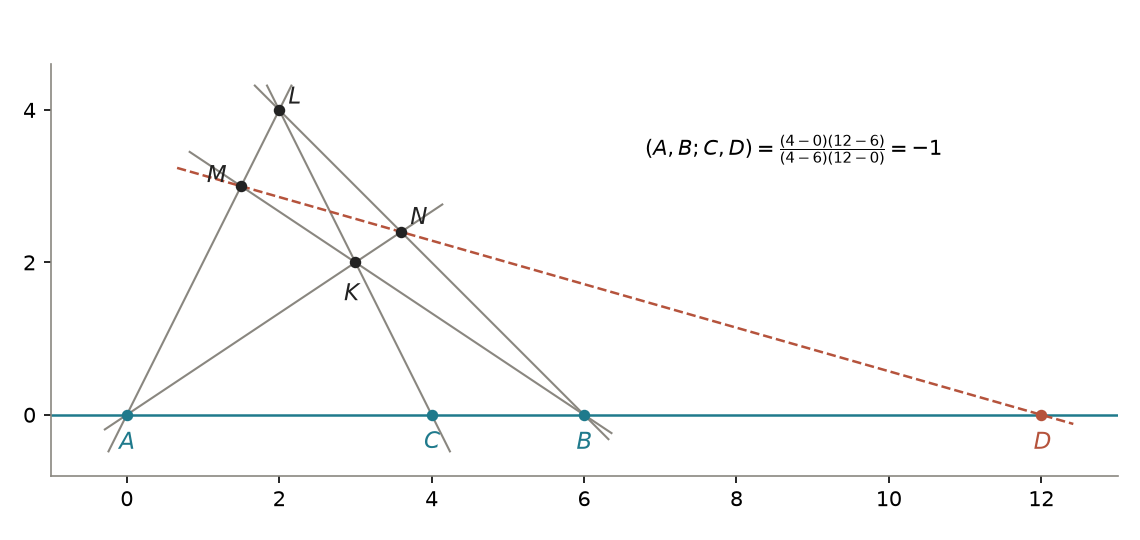
\includegraphics[width=.9\linewidth]{figuras/proyectivas/c1_conjugado_armonico.png}
\caption{Construcción del conjugado armónico con el cuadrilátero completo \(L,M,N,K\):
\(A=(0,0)\), \(B=(6,0)\), \(C=(4,0)\), \(L=(2,4)\), \(K=(3,2)\), \(M=BK\cap LA=(1{,}5;\ 3)\),
\(N=AK\cap LB=(3{,}6;\ 2{,}4)\) y \(D=MN\cap AB=(12,0)\). Generada con
\texttt{apunte/scripts/capc1\_conjugado\_armonico.py}.}
\label{fig:c1-conjugado-armonico}
\end{figure}

\begin{ejemplo}[Conjugado armónico con coordenadas]\label{ej:c1-conjugado-armonico}
Sean \(A=(0,0)\), \(B=(6,0)\) y \(C=(4,0)\) sobre el eje \(x\), con la abscisa como coordenada
afín. La fórmula da \(d=\dfrac{6\cdot4}{2\cdot4-6}=12\), y en efecto
\[
  (0,6;4,12)=\frac{(4-0)(12-6)}{(4-6)(12-0)}=\frac{24}{-24}=-1 .
\]
\(C\) está dentro de \(AB\), más cerca de \(B\), y \(D\) quedó afuera, del lado de \(B\). La
construcción de la figura~\ref{fig:c1-conjugado-armonico} da lo mismo con productos cruz
en homogéneas: con \(L=(2,4)\) y \(K=(3,2)\), el punto medio de \(LC\), resultan
\(M=(1{,}5;\ 3)\), \(N=(3{,}6;\ 2{,}4)\), y la recta \(MN\), de pendiente \(-2/7\), corta al eje en
\(x=1{,}5+3\cdot\tfrac72=12\). Por último, la homografía \(f(x)=\dfrac{2x+1}{x+3}\) del
ejemplo~\ref{ej:c1-razon-doble} lleva \(0,6,4,12\) a \(\tfrac13,\tfrac{13}9,\tfrac97,\tfrac53\), y
\[
  \Bigl(\tfrac13,\tfrac{13}9;\tfrac97,\tfrac53\Bigr)
  =\frac{\bigl(\tfrac97-\tfrac13\bigr)\bigl(\tfrac53-\tfrac{13}9\bigr)}
        {\bigl(\tfrac97-\tfrac{13}9\bigr)\bigl(\tfrac53-\tfrac13\bigr)}
  =\frac{\tfrac{20}{21}\cdot\tfrac29}{-\tfrac{10}{63}\cdot\tfrac43}
  =\frac{40/189}{-40/189}=-1 :
\]
la cuaterna sigue siendo armónica, aunque \(C\) ya no divide al segmento en la misma razón.
\end{ejemplo}

En una homología armónica (sección~\ref{sec:homografia-fijos}), cada punto y su imagen son
conjugados armónicos respecto del centro y del corte de su recta con el eje; es lo que
comprueba la razón doble \((D,D';O,X)=-1\) en el ejercicio del pentágono de la unidad
interactiva.

\begin{atencion}[Tres \enquote{conjugados} distintos]
El conjugado armónico no tiene relación con la conjugación de matrices
(sección~\ref{sec:conjugacion}) ni con el conjugado complejo
(sección~\ref{sec:conjugado-complejo}): es la misma palabra para tres ideas distintas. El
glosario de la sección~\ref{sec:glosario} las separa.
\end{atencion}

\subsection{Cuatro puntos determinan la homografía}\label{sec:cuatro-puntos}

¿Cuántos puntos de una pared hay que reconocer en su foto para poder deshacer la perspectiva?
Con tres alcanzaba para una afinidad (proposición~\ref{prop:06-tres-puntos}); la perspectiva pide
uno más.

\paragraph{Conteo.} Cada correspondencia \(p_i\mapsto p_i'\) aporta dos ecuaciones
(\(X/W=x_i'\), \(Y/W=y_i'\)). Cuatro correspondencias dan ocho ecuaciones para ocho
incógnitas. La condición es que ni entre los cuatro puntos de partida ni entre los cuatro de
llegada haya tres alineados (con el determinante se verifica).

\paragraph{Construcción.} En lugar de resolver el sistema \(8\times8\) se pasa por un
\emph{cuadrilátero patrón}:
\[
  e_1=\begin{pmatrix}1\\0\\0\end{pmatrix},\quad
  e_2=\begin{pmatrix}0\\1\\0\end{pmatrix},\quad
  e_3=\begin{pmatrix}0\\0\\1\end{pmatrix},\quad
  e_4=\begin{pmatrix}1\\1\\1\end{pmatrix}=e_1+e_2+e_3 .
\]
Dados cuatro puntos \(p_1,p_2,p_3,p_4\) sin tres alineados, se busca una matriz \(K\) con
\(Ke_i\sim p_i\) para \(i=1,\dots,4\):
\begin{enumerate}
  \item Se forma \(M=[\,p_1\ p_2\ p_3\,]\) con los tres primeros puntos como columnas. Como
  \(Me_i\) es la \(i\)-ésima columna, ya se cumple \(Me_i=p_i\) para \(i\le3\). Pero
  \(Me_4=p_1+p_2+p_3\), que en general no es \(p_4\).
  \item Como cada columna representa su punto \emph{a menos de escala}, se la puede
  multiplicar por un número sin cambiar a dónde va \(e_i\). Se eligen \(\mu_1,\mu_2,
  \mu_3\) tales que
  \[
    \mu_1p_1+\mu_2p_2+\mu_3p_3=p_4
    \qquad\Longleftrightarrow\qquad
    \mu=M^{-1}p_4 .
  \]
  \item La matriz buscada es \(K=[\,\mu_1p_1\ \ \mu_2p_2\ \ \mu_3p_3\,]\):
  las tres primeras columnas siguen representando \(p_1,p_2,p_3\) y su suma es \(p_4\).
\end{enumerate}

\begin{resultado}[Homografía que lleva un cuadrilátero sobre otro]
Sean \(K_1\) la matriz del patrón para los puntos de partida \(p_1,\dots,p_4\) y \(K_2\) la
del patrón para los puntos de llegada \(p_1',\dots,p_4'\). Entonces
\[
  \boxed{H=K_2K_1^{-1}}
\]
es la única homografía (a menos de escala) con \(Hp_i\sim p_i'\), \(i=1,\dots,4\).
Se lee de derecha a izquierda: \(K_1^{-1}\) lleva el cuadrilátero de partida al patrón, y
\(K_2\) lleva el patrón al cuadrilátero de llegada.
\end{resultado}

Es el mismo esquema de la afinidad determinada por tres puntos de control
(proposición~\ref{prop:06-tres-puntos}, \(A=P'P^{-1}\)), con un punto más para absorber la
perspectiva. Los \(\mu_i\), invisibles punto a punto, son precisamente los
grados de libertad que faltaban.

\subsection{Puntos fijos y rectas fijas de una homografía}\label{sec:homografia-fijos}

¿Hay algún punto que una homografía deje en su lugar? Saberlo dice qué tipo de
transformación es: un giro alrededor de un punto, un espejo, o una perspectiva más general.

Los puntos fijos de una homografía son autovectores; la teoría general de autovalores y
autovectores se desarrolla en las secciones~\ref{sec:autovalores} y~\ref{sec:autovalores-geom}.
Un punto \(p\) es fijo si
\(Hp\sim p\), es decir si existe \(\lambda\neq0\) con \(Hp=\lambda p\): \emph{los puntos
fijos son los autovectores reales de \(H\)}. Se calculan así: se buscan las raíces reales de
\(\det(H-\lambda I)=0\) y, para cada una, se toma el producto cruz de dos filas de
\(H-\lambda I\). Ese vector es perpendicular a las dos filas; cuando \(H-\lambda I\) tiene
rango \(2\), la tercera fila es combinación de las otras dos y el producto cruz anula a toda
la matriz, es decir, resuelve \((H-\lambda I)p=0\).

\begin{resultado}[Existencia de punto fijo]
Toda homografía del plano tiene al menos un punto fijo, porque el polinomio característico
es de grado \(3\). Es ordinario si el autovector tiene tercera coordenada no nula, e ideal
(una dirección fija) si la tercera coordenada es cero. Una raíz doble con producto cruz de
filas nulo significa toda una recta de puntos fijos.
\end{resultado}

\paragraph{Rectas fijas.} Como las rectas se transforman con \(H^{-T}\), una recta es fija
si es autovector de \(H^{T}\); se encuentra con el producto cruz de dos filas de
\(H^{T}-\lambda I\) (o sea, de dos columnas de \(H-\lambda I\)). Una recta fija de autovalor
\(\lambda'\) pasa por todos los puntos fijos de autovalor \(\lambda\neq\lambda'\).

\paragraph{Clasificación por autovalores.}
\begin{itemize}
  \item \textbf{Tres autovalores reales distintos:} tres puntos fijos no alineados y tres
  rectas fijas, los lados de ese triángulo.
  \item \textbf{Un real y dos complejos conjugados} (\(\lambda\) y \(\bar\lambda\), en el sentido de la sección~\ref{sec:conjugado-complejo})\textbf{:} un único punto fijo real y una única
  recta fija real que no pasa por él. En coordenadas adecuadas es una rotación alrededor del
  punto fijo, con la recta fija en el papel de recta ideal.
  \item \textbf{Un autovalor doble con producto cruz de filas nulo:} una recta entera de
  puntos fijos (el \emph{eje}) y un punto fijo aislado (el \emph{centro}) con el otro
  autovalor. Es una \emph{homología}. Si los dos autovalores son opuestos, \(H^2\sim I\): la
  homología es \emph{armónica}, una involución, como una reflexión.
\end{itemize}

\subsection{Aplicación: enderezar la foto de una fachada}\label{sec:c1-aplicacion-fachada}

Tenemos una foto de una pared, sacada de costado y un poco desde abajo, y queremos saber cuánto
mide una puerta de esa pared sin ir a medirla. De la pared conocemos una sola cosa: tiene una
ventana rectangular de \(1{,}50\ \mathrm{m}\) de ancho por \(1{,}20\ \mathrm{m}\) de alto, que
medimos con una cinta. En la foto la ventana no sale rectangular: es un cuadrilátero con los
lados opuestos inclinados distinto, y la puerta, que está más lejos de la cámara, sale más
chica de lo que es. ¿Podemos usar la ventana como patrón para enderezar la pared entera y medir
la puerta sobre la pared enderezada? Por la sección~\ref{sec:cuatro-puntos}, sí: los cuatro
vértices de la ventana, en la foto y en la pared, determinan la homografía que lleva una a la
otra.

\begin{idea}[Esto lo vas a usar en Topografía]
Enderezar la foto de una superficie plana a partir de puntos cuyas medidas se conocen se llama
\emph{rectificar} la foto. Sirve para dibujar fachadas y para medir sobre cualquier superficie
plana fotografiada sin recorrerla con la cinta.
\end{idea}

\paragraph{Dos sistemas de coordenadas.} En la foto usamos, como en la ortofoto del
capítulo~\ref{cap:afines} (sección~\ref{sec:aplicacion-ortofoto}), la columna \(c\) y la fila
\(f\) de cada píxel, con origen en el vértice superior izquierdo y \emph{la fila creciendo hacia
abajo}. En la pared usamos metros: \(x\) hacia la derecha e \(y\) hacia arriba, con origen en el
vértice inferior izquierdo de la ventana. Buscamos la matriz \(H\) de \(3\times3\) que lleva
\((c,f,1)^T\) a un múltiplo de \((x,y,1)^T\).

\paragraph{Datos.} Son sintéticos, generados por el script
\texttt{apunte/scripts/c1\_proyectivas.py}. El script parte de una pared de juguete (la ventana de
\(1{,}50\times1{,}20\ \mathrm{m}\) y una puerta de \(0{,}90\times2{,}05\ \mathrm{m}\)), la
fotografía con una homografía conocida, la que produciría una cámara de distancia focal
\(1300\) píxeles girada \(40^\circ\) respecto de la pared y levantada \(12^\circ\), y a cada
vértice le suma un error al azar de medio píxel (semilla \(2026\)), redondeando al décimo de
píxel, como cuando se marcan los vértices a mano sobre la pantalla. Las medidas de la puerta no
entran en el cálculo: las guardamos para comparar al final.
\begin{center}
\begin{tabular}{lcc}
\toprule
punto & foto \((c;\,f)\) (px) & pared \((x;\,y)\) (m)\\
\midrule
\(V_1\) ventana, abajo a la izquierda & \(93{,}3;\ 692{,}1\) & \(0;\ 0\)\\
\(V_2\) ventana, abajo a la derecha & \(567{,}7;\ 730{,}9\) & \(1{,}50;\ 0\)\\
\(V_3\) ventana, arriba a la derecha & \(581{,}0;\ 405{,}2\) & \(1{,}50;\ 1{,}20\)\\
\(V_4\) ventana, arriba a la izquierda & \(139{,}2;\ 290{,}2\) & \(0;\ 1{,}20\)\\
\midrule
\(P_1\) puerta, abajo a la izquierda & \(768{,}2;\ 997{,}9\) & a medir\\
\(P_2\) puerta, abajo a la derecha & \(935{,}5;\ 985{,}7\) & a medir\\
\(P_3\) puerta, arriba a la derecha & \(925{,}3;\ 516{,}3\) & a medir\\
\(P_4\) puerta, arriba a la izquierda & \(770{,}9;\ 477{,}9\) & a medir\\
\bottomrule
\end{tabular}
\end{center}

\begin{figure}[htbp]
\centering
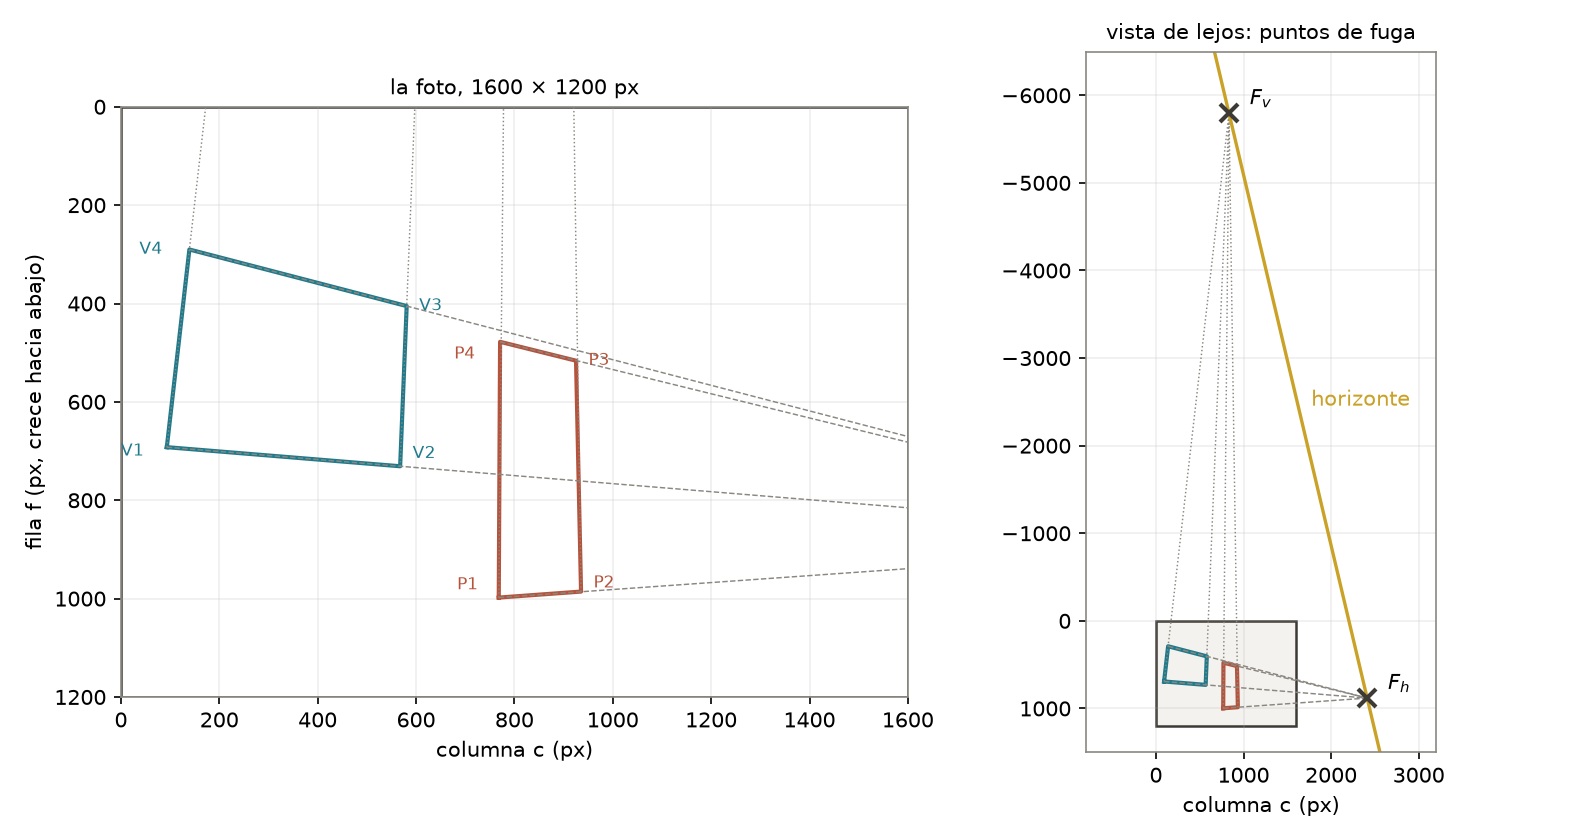
\includegraphics[width=\linewidth]{figuras/proyectivas/c1_fachada_foto.png}
\caption{Izquierda: la foto sintética de la fachada, con la ventana (\(V_1\) a \(V_4\)) y la
puerta (\(P_1\) a \(P_4\)); en gris, las prolongaciones de los lados. Derecha: la misma foto vista
de lejos. Los lados que en la pared son horizontales se cortan en el punto de fuga \(F_h\), los
verticales en \(F_v\), y la recta que los une es el horizonte, la recta que \(H\) manda al
infinito. Generada con \texttt{apunte/scripts/c1\_proyectivas.py}.}
\label{fig:c1-fachada-foto}
\end{figure}

\paragraph{Lo que la foto no respeta.} Medidos contra la horizontal de la foto, el lado de
abajo de la ventana baja \(4{,}68^\circ\) hacia la derecha y el de arriba \(14{,}59^\circ\): en
la pared son paralelos y en la foto no. Los lados verticales forman \(83{,}48^\circ\) y
\(87{,}66^\circ\) con la horizontal: tampoco son paralelos. ¿Dónde se cortan? Con las rectas en
coordenadas homogéneas, la recta por dos puntos y el punto común a dos rectas se calculan con
el producto cruz. Los lados de abajo y de arriba se cortan en el punto de fuga
\(F_h=(2411{,}6;\ 881{,}7)\), fuera de la foto a la derecha; los lados verticales, en
\(F_v=(834{,}2;\ -5795{,}1)\), muy por encima de la foto, porque la cámara mira hacia arriba
(figura~\ref{fig:c1-fachada-foto}). Si quisiéramos medir la puerta con una regla sobre la foto,
usando como escala la ventana (\(1{,}50\ \mathrm{m}\) en los \(476{,}0\) px del lado de abajo y
\(1{,}20\ \mathrm{m}\) en los \(404{,}5\) px del lado izquierdo), los \(167{,}7\) px del lado de
abajo de la puerta darían \(0{,}53\ \mathrm{m}\) y los \(520{,}0\) px del lado izquierdo,
\(1{,}54\ \mathrm{m}\): \(37\ \mathrm{cm}\) de menos en el ancho y \(51\ \mathrm{cm}\) en el
alto. En la foto la escala cambia de un punto a otro.

\paragraph{Ocho ecuaciones lineales.} Escribimos la homografía buscada coordenada por
coordenada, con \(h_{ij}\) la entrada de la fila \(i\) y la columna \(j\) de \(H\):
\[
  x=\frac{h_{11}c+h_{12}f+h_{13}}{h_{31}c+h_{32}f+h_{33}},
  \qquad
  y=\frac{h_{21}c+h_{22}f+h_{23}}{h_{31}c+h_{32}f+h_{33}} .
\]
Como \(H\) y \(\mu H\) dan la misma transformación, podemos elegir la escala: fijamos
\(h_{33}=1\). (Esa elección solo falla si \(h_{33}=0\), cuando el píxel \((0,0)\) va al infinito;
no es el caso de una foto en la que la pared ocupa el cuadro.) Pasando el denominador a la
izquierda y ordenando, cada vértice da dos ecuaciones \emph{lineales} en las ocho incógnitas:
\[
\begin{aligned}
  h_{11}c+h_{12}f+h_{13}-h_{31}\,c\,x-h_{32}\,f\,x&=x,\\
  h_{21}c+h_{22}f+h_{23}-h_{31}\,c\,y-h_{32}\,f\,y&=y .
\end{aligned}
\]
Es la \emph{transformación lineal directa} (en inglés, DLT): directa porque el problema, que
parecía de cocientes, quedó como un sistema lineal común. Por ejemplo, \(V_2\), con
\((c;\,f)=(567{,}7;\ 730{,}9)\) y \((x;\,y)=(1{,}5;\ 0)\), aporta las filas
\[
\begin{aligned}
  567{,}7\,h_{11}+730{,}9\,h_{12}+h_{13}-851{,}55\,h_{31}-1096{,}35\,h_{32}&=1{,}5,\\
  567{,}7\,h_{21}+730{,}9\,h_{22}+h_{23}&=0 .
\end{aligned}
\]
Con los cuatro vértices de la ventana queda un sistema de \(8\times8\), con solución única
porque no hay tres vértices alineados. Resulta
\[
  H=10^{-3}\begin{pmatrix}
  2{,}5710&0{,}2936&-443{,}09\\
  0{,}2342&-2{,}8633&1959{,}87\\
  -0{,}4539&0{,}1072&1000
  \end{pmatrix}.
\]
El script comprueba que el método del patrón de la sección~\ref{sec:cuatro-puntos},
\(H=K_2K_1^{-1}\) normalizada con \(h_{33}=1\), da la misma matriz, y que \(H\) lleva los cuatro
vértices de la ventana a \((0;\ 0)\), \((1{,}5;\ 0)\), \((1{,}5;\ 1{,}2)\) y \((0;\ 1{,}2)\).

\paragraph{El horizonte.} La tercera fila de \(H\) es la recta de la foto que se va al infinito
(sección~\ref{sec:jerarquia}): \(-0{,}4539\,c+0{,}1072\,f+1000=0\). Tiene que pasar por \(F_h\) y
por \(F_v\), porque las imágenes de los lados de la ventana son paralelas y sus puntos comunes
están en el infinito. El script calcula la recta \(F_h\times F_v\) y comprueba que es la misma.
Es el horizonte dorado de la figura~\ref{fig:c1-fachada-foto}.

\paragraph{Las rectas siguen rectas, las razones simples no.} Tomemos en la foto el punto medio
del borde izquierdo de la puerta, \((769{,}55;\ 737{,}9)\), a mitad de camino entre \(P_1\) y
\(P_4\). \(H\) lo lleva a \((2{,}401;\ 0{,}037)\), y el determinante de las ternas de las tres
imágenes (los extremos y ese punto) da cero: siguen alineadas. Pero el punto ya no está a mitad
de altura: queda a \(0{,}480\) del recorrido, contando desde abajo. Lo que la foto muestra como
mitad, en la pared no lo es.

\paragraph{La razón doble se conserva.} Prolonguemos en la foto el lado de abajo de la ventana,
la recta del alféizar (el borde inferior de la ventana). Corta a los bordes verticales de la
puerta en dos puntos, \(Q\) y \(R\), que se calculan otra vez con productos cruz. Sobre esa recta
de la foto, la columna \(c\) sirve de coordenada afín, y los cuatro puntos \(V_1,V_2,Q,R\) tienen
\(c=93{,}3;\ 567{,}7;\ 769{,}5;\ 930{,}6\). En la pared enderezada caen sobre la recta \(y=0\), en
\(x=0;\ 1{,}5;\ 2{,}401;\ 3{,}296\). La razón doble
(definición~\ref{def:c1-razon-doble}) vale
\[
  (V_1,V_2;Q,R)=1{,}4523
\]
en las dos, con todas las cifras que calcula el script, como asegura la
proposición~\ref{prop:c1-razon-doble}. La razón simple, en cambio, cambia: \(V_1V_2/V_1Q\) es
\(0{,}702\) en la foto y \(0{,}625\) en la pared. En la pared verdadera, con los bordes de la
puerta en \(x=2{,}4\) y \(x=3{,}3\), la razón doble es \(16/11\approx1{,}4545\); la diferencia con
\(1{,}4523\) es el error de medio píxel de los vértices marcados.

\begin{figure}[htbp]
\centering
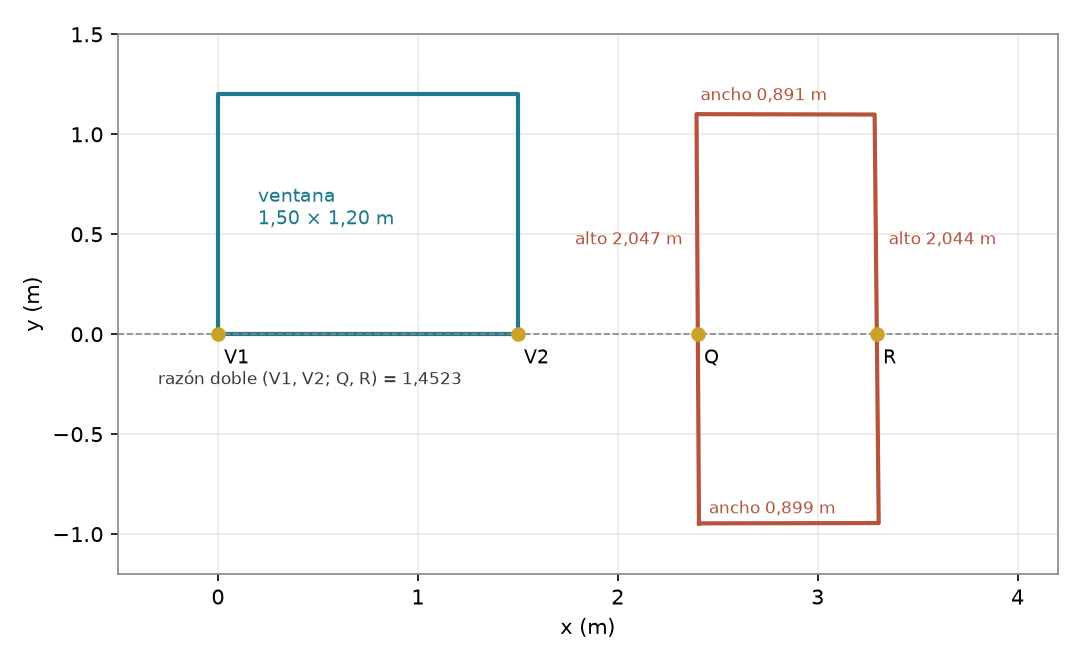
\includegraphics[width=.92\linewidth]{figuras/proyectivas/c1_fachada_enderezada.png}
\caption{La pared enderezada por \(H\): la ventana vuelve a ser el rectángulo de
\(1{,}50\times1{,}20\ \mathrm{m}\) y la puerta aparece con sus medidas. Los puntos dorados son
\(V_1\), \(V_2\), \(Q\) y \(R\) sobre la recta \(y=0\), la del alféizar, con la misma razón doble
que en la foto. Generada con \texttt{apunte/scripts/c1\_proyectivas.py}.}
\label{fig:c1-fachada-enderezada}
\end{figure}

\paragraph{La puerta, medida.} Aplicando \(H\) a \(P_1,\dots,P_4\) obtenemos, en metros,
\[
  P_1\mapsto(2{,}406;\ -0{,}946),\quad P_2\mapsto(3{,}306;\ -0{,}945),\quad
  P_3\mapsto(3{,}285;\ 1{,}099),\quad P_4\mapsto(2{,}394;\ 1{,}101).
\]
Los lados de abajo y de arriba miden \(0{,}899\) y \(0{,}891\ \mathrm{m}\), y los bordes
izquierdo y derecho \(2{,}047\) y \(2{,}044\ \mathrm{m}\)
(figura~\ref{fig:c1-fachada-enderezada}). Promediando, la puerta mide \(0{,}895\ \mathrm{m}\) de
ancho por \(2{,}045\ \mathrm{m}\) de alto. Las medidas con que el script armó la pared son
\(0{,}90\) y \(2{,}05\ \mathrm{m}\): la diferencia, de unos \(5\ \mathrm{mm}\), viene del medio
píxel de error al marcar los ocho vértices. Los bordes verticales de la puerta, que en la foto
forman entre sí \(1{,}54^\circ\), en la pared enderezada forman \(0{,}23^\circ\): casi
paralelos, y lo que falta también es error de marcado.

\begin{atencion}[Una pared, no un edificio]
La homografía endereza \emph{un plano}. Todo lo que está sobre la pared (ventanas, puertas,
juntas de ladrillos) queda bien medido; lo que sobresale de ella (un balcón, el marco de la
ventana si está hundido) no, porque no está en el plano que fijaron los cuatro vértices.
\end{atencion}

\unidadInteractiva{05_proyectivas}{Proyectivas: la perspectiva de una cámara y el pentágono regular}{Explorá: en «caso precargado» elegí «foto de dron: cámara inclinada (k)» y mové el deslizador «k (inclinación, h\(_{32}\))». Con \(k=0\) la tercera fila de la matriz es \((0\ \ 0\ \ 1)\): la transformación es afín y las rectas \(x=\) constante siguen paralelas. Con cualquier otro \(k\) convergen al punto de fuga marcado con una cruz, como los bordes verticales de la puerta en la foto de la fachada.}

\section{En profundidad}

Resolvemos caso por caso el ejercicio del pentágono regular.

\subsection{El ejercicio del pentágono regular}

\begin{enunciado}[El quinto vértice de un pentágono regular]
Tomar un pentágono \emph{regular} \(ABCDE\). Una transformación proyectiva queda definida
por cuatro puntos, así que se prescriben cuatro vértices y sus imágenes (otros cuatro
vértices) y se pregunta \emph{a dónde cae el quinto}. Hay tres casos, y sus combinaciones
con las rotaciones del pentágono:
\begin{enumerate}[label=(\alph*)]
  \item no intercambiar ningún vértice: solo \enquote{correr} el pentágono;
  \item intercambiar dos vértices adyacentes;
  \item intercambiar dos vértices no adyacentes.
\end{enumerate}
Para cada transformación, determinar si tiene punto fijo (un autovector de la matriz).
\end{enunciado}

Se toma el pentágono regular inscripto en la circunferencia unidad,
centrado en el origen y con un vértice arriba. Conviene centrarlo en el origen:
en el caso más simple el punto fijo es el centro, cuyo autovector es \((0,0,1)^T\).
\begin{gather*}
  A=(0,\,1),\qquad B=(-0{,}9511;\ 0{,}3090),\qquad C=(-0{,}5878;\ -0{,}8090),\\
  D=(0{,}5878;\ -0{,}8090),\qquad E=(0{,}9511;\ 0{,}3090).
\end{gather*}
Las coordenadas son irracionales (\(\cos72^\circ=\frac{\sqrt5-1}{4}\)), así que las
matrices se calculan con cuatro decimales y se verifican en NumPy (apéndice~\ref{ap:pentagono}).
En los tres casos se usa \(H=K_2K_1^{-1}\) con \(K_1\) el patrón de \(ABCD\), y se
normaliza \(h_{33}=1\).

\begin{center}
\begin{tikzpicture}[scale=1.9]
  \draw[linegray!40,very thin] (-1.6,-1.4) grid[step=.5] (1.6,1.3);
  \draw[axisline,-{Latex[length=2.2mm]}] (-1.7,0)--(1.7,0) node[right] {$x$};
  \draw[axisline,-{Latex[length=2.2mm]}] (0,-1.45)--(0,1.35) node[above] {$y$};
  \draw[linegray,densely dotted] (0,0) circle (1);
  \draw[teal,line width=1.05pt,fill=teallight!45] (0,1)--(-0.9511,0.3090)--(-0.5878,-0.8090)--(0.5878,-0.8090)--(0.9511,0.3090)--cycle;
  \foreach \p/\n/\pos in {(0,1)/A/above,(-0.9511,0.3090)/B/left,(-0.5878,-0.8090)/C/{below left},(0.5878,-0.8090)/D/{below right},(0.9511,0.3090)/E/right}
    \fill[teal] \p circle (1.2pt) node[\pos,font=\small,text=tealdark] {$\n$};
  \fill[ink] (0,0) circle (1.2pt) node[below right,font=\scriptsize] {$O$};
  % caso (c): imagen C B A D E'
  \draw[rust,line width=1pt] (-0.5878,-0.8090)--(-0.9511,0.3090)--(0,1)--(0.5878,-0.8090)--(0,-1.2361)--cycle;
  \fill[rust] (0,-1.2361) circle (1.4pt) node[right=2pt,font=\small,text=rust,labelback] {$E'_c=(0;\ -1{,}2361)$};
  % eje BD
  \draw[dashed,tealdark,line width=.8pt] ($(-0.9511,0.3090)!-0.35!(0.5878,-0.8090)$)--($(-0.9511,0.3090)!1.35!(0.5878,-0.8090)$) node[right,font=\scriptsize,text=tealdark] {eje $BD$};
  % recta AC (contiene al centro)
  \draw[dotted,gold!70!black,line width=.8pt] ($(0,1)!-0.3!(-0.5878,-0.8090)$)--($(0,1)!1.3!(-0.5878,-0.8090)$);
  \node[gold!60!black,font=\scriptsize,labelback,anchor=east] at (-0.55,-1.3) {hacia $O_c=(-1{,}54;\ -3{,}74)$};
\end{tikzpicture}
\end{center}

\paragraph{(a) Sin intercambio: \(A\mapsto B,\ B\mapsto C,\ C\mapsto D,\ D\mapsto E\).}
Los cuatro pares son compatibles con la rotación de \(72^\circ\) alrededor de \(O\), que es
una isometría y por lo tanto una homografía. Como la homografía es única, \emph{es} esa
rotación:
\[
  H_a=\begin{pmatrix}0{,}3090&-0{,}9511&0\\0{,}9511&0{,}3090&0\\0&0&1\end{pmatrix},
  \qquad H_aE=A .
\]
El quinto vértice cae en \(A\): el pentágono regular sí \enquote{cierra}. Autovalores \(1\) y
\(e^{\pm i\,72^\circ}\); único punto fijo real \(O=(0,0)\), obtenido como producto cruz de
las dos primeras filas de \(H_a-I\):
\[
  (-0{,}691;\ -0{,}951;\ 0)\times(0{,}951;\ -0{,}691;\ 0)=(0;\ 0;\ 1{,}382)\sim(0,0,1)^T .
\]
La recta ideal es fija (es afín) y ninguna otra.

\paragraph{(b) Intercambio de adyacentes: \(A\leftrightarrow B\), \(C\) y \(D\) quietos.}
\[
  H_b=\begin{pmatrix}-5{,}8541&-4{,}9798&-4{,}0287\\0&-1&3{,}9271\\0&8{,}4721&1\end{pmatrix},
  \qquad E\mapsto E'_b=(-3{,}0777;\ 1{,}0000).
\]
Autovalores \(5{,}8541\) (simple) y \(-5{,}8541\) (doble). Para el doble, el producto cruz de
cualquier par de filas de \(H_b+5{,}8541I\) es nulo: hay toda una recta de puntos fijos, que es
la recta \(CD\) (\(y=-0{,}8090\)), lógico porque \(C\) y \(D\) quedan quietos. El autovalor
simple da el centro, \(O_b=(-0{,}5878;\ 0{,}5729)\), que está sobre la recta \(AB\) (la recta
\(AB\) va a sí misma porque sus extremos se intercambian). Como los autovalores son
opuestos, \(H_b^2\sim I\): es una \emph{homología armónica}, un \enquote{espejo proyectivo} de eje
\(CD\) y centro \(O_b\). La recta que se va al infinito es \(y=-0{,}1180\), que
\emph{atraviesa} el pentágono (\(W\) vale \(9{,}47;\ 3{,}62;\ -5{,}85;\ -5{,}85;\ 3{,}62\) en
\(A,\dots,E\)): los lados \(BC\) y \(DE\) la cruzan y la imagen del pentágono se parte en
dos semirrectas por lado.

\paragraph{(c) Intercambio de no adyacentes: \(A\leftrightarrow C\), \(B\) y \(D\) quietos.}
\[
  H_c=\begin{pmatrix}0{,}4271&-0{,}5878&-0{,}2245\\-1{,}0368&-0{,}5729&-0{,}5451\\0{,}2775&0{,}3820&1\end{pmatrix},
  \qquad E\mapsto E'_c=(0;\ -1{,}2361).
\]
Autovalores \(0{,}8541\) (doble) y \(-0{,}8541\). Eje de puntos fijos: la recta \(BD\)
(\(0{,}7265x+y+0{,}3820=0\)); centro \(O_c=(-1{,}5388;\ -3{,}7361)\), sobre la prolongación de
\(AC\), obtenido como producto cruz de las dos primeras filas de \(H_c+0{,}8541I\):
\((1{,}2812;\ -0{,}5878;\ -0{,}2245)\times(-1{,}0368;\ 0{,}2812;\ -0{,}5451)=(0{,}3835;\ 0{,}9311;\ -0{,}2492)\sim
(-1{,}5388;\ -3{,}7361;\ 1)\). Otra vez \(H_c^2\sim I\): homología armónica de eje \(BD\). El
quinto vértice cae en \(E'_c=(0;\ -1{,}2361)\), sobre el eje de simetría, y como la recta que se
va al infinito (\(0{,}2775x+0{,}3820y+1=0\)) no toca el pentágono (\(W>0\) en los cinco
vértices), la imagen es el pentágono \(CBADE'_c\) de la figura, no convexo pero entero.

\paragraph{Combinaciones con rotaciones.} Cualquier otra correspondencia de cuatro vértices
sobre cuatro vértices es una de las tres anteriores seguida de una rotación \(H_a^k\), o una
reflexión del pentágono. Por ejemplo \(A\mapsto E,\ B\mapsto D,\ C\mapsto C,\ D\mapsto B\)
es la reflexión respecto del eje \(OC\) (afín, \(E\mapsto A\), todo el eje fijo y la
dirección perpendicular como punto fijo ideal). Componer (b) con la rotación da un único punto
fijo real y dos autovalores complejos; componer (c) con la rotación da tres autovalores
reales distintos y un triángulo invariante. El script de la sección~\ref{ap:pentagono}
permite verificarlo.

\begin{resultado}[Respuestas a la consigna]
\begin{itemize}
  \item Con \(A,B,C,D\) fijos como puntos de partida, sus imágenes son cuatro vértices
  distintos elegidos en orden entre cinco: hay \(5\cdot4\cdot3\cdot2=120\) correspondencias,
  todas bien definidas (el pentágono es convexo, nunca hay tres vértices alineados). Componer
  con las \(10\) simetrías del pentágono (\(5\) rotaciones y \(5\) reflexiones) agrupa esas
  \(120\) correspondencias en \(120/10=12\) familias. Dentro de una familia las homografías
  difieren en una simetría, así que basta estudiar un representante por familia: (a) está en
  la familia de la identidad, y (b) y (c) son representantes de otras dos.
  \item (a) es la rotación; el quinto vértice cae en un vértice y el punto fijo es el centro.
  \item (b) y (c) son homologías armónicas: una recta entera de puntos fijos, la que une los
  dos vértices que quedan quietos (el lado \(CD\) en (b), la diagonal \(BD\) en (c)), más un
  centro; el quinto vértice cae fuera del pentágono, en
  \((-3{,}08;\ 1)\) y \((0;\ -1{,}24)\) respectivamente. En (b) la imagen se parte; en (c) no.
  \item Siempre hay punto fijo: es el autovector real de \(H\), y se calcula con el producto
  cruz de dos filas de \(H-\lambda I\).
\end{itemize}
\end{resultado}

% Apéndice: pentágono regular: cuentas y script
\subsection{El pentágono}\label{cap:pentagono}\label{ap:pentagono}

Ternas homogéneas (cuatro decimales):
\[
A=\begin{pmatrix}0\\1\\1\end{pmatrix},\
B=\begin{pmatrix}-0{,}9511\\0{,}3090\\1\end{pmatrix},\
C=\begin{pmatrix}-0{,}5878\\-0{,}8090\\1\end{pmatrix},\
D=\begin{pmatrix}0{,}5878\\-0{,}8090\\1\end{pmatrix},\
E=\begin{pmatrix}0{,}9511\\0{,}3090\\1\end{pmatrix}.
\]

\subsubsection{Verificación de los tres casos}
\begin{center}\small
\begin{tabularx}{\textwidth}{>{\bfseries}l X X X}
\toprule
& (a) \(ABCD\to BCDE\) & (b) \(ABCD\to BACD\) & (c) \(ABCD\to CBAD\)\\
\midrule
\(HA\) & \(B\), \(W=1\) & \(B\), \(W=9{,}4721\) & \(C\), \(W=1{,}3820\)\\
\(HB\) & \(C\), \(W=1\) & \(A\), \(W=3{,}6180\) & \(B\), \(W=0{,}8541\)\\
\(HC\) & \(D\), \(W=1\) & \(C\), \(W=-5{,}8541\) & \(A\), \(W=0{,}5279\)\\
\(HD\) & \(E\), \(W=1\) & \(D\), \(W=-5{,}8541\) & \(D\), \(W=0{,}8541\)\\
\(HE\) & \(A\), \(W=1\) & \((-3{,}0777;\ 1)\), \(W=3{,}6180\) & \((0;\ -1{,}2361)\), \(W=1{,}3820\)\\
recta al infinito & ideal & \(y=-0{,}1180\) & \(0{,}2775x+0{,}3820y+1=0\)\\
autovalores & \(1,\ e^{\pm i72^\circ}\) & \(5{,}8541;\ -5{,}8541\ (\times2)\) &
\(-0{,}8541;\ 0{,}8541\ (\times2)\)\\
puntos fijos & \(O=(0,0)\) & eje \(CD\); centro \((-0{,}5878;\ 0{,}5729)\) &
eje \(BD\); centro \((-1{,}5388;\ -3{,}7361)\)\\
tipo & rotación (afín) & homología armónica, imagen partida & homología armónica\\
\bottomrule
\end{tabularx}
\end{center}

\subsubsection{Autovector por producto cruz, caso (c)}
Polinomio característico de \(H_c\): \(\lambda^3-0{,}8541\lambda^2-0{,}7295\lambda+0{,}6231\),
raíces \(0{,}8541\) (doble) y \(-0{,}8541\). Para \(\lambda=-0{,}8541\),
\[
H_c+0{,}8541\,I=\begin{pmatrix}1{,}2812&-0{,}5878&-0{,}2245\\-1{,}0368&0{,}2812&-0{,}5451\\0{,}2775&0{,}3820&1{,}8541\end{pmatrix},
\]
\[
\text{fila}_1\times\text{fila}_2=
\begin{pmatrix}(-0{,}5878)(-0{,}5451)-(-0{,}2245)(0{,}2812)\\(-0{,}2245)(-1{,}0368)-(1{,}2812)(-0{,}5451)\\(1{,}2812)(0{,}2812)-(-0{,}5878)(-1{,}0368)\end{pmatrix}
=\begin{pmatrix}0{,}3835\\0{,}9311\\-0{,}2492\end{pmatrix}\sim\begin{pmatrix}-1{,}5388\\-3{,}7361\\1\end{pmatrix}.
\]
Comprobación:
\[
  H_c\begin{pmatrix}-1{,}5388\\-3{,}7361\\1\end{pmatrix}=\begin{pmatrix}1{,}3143\\3{,}1909\\-0{,}8541\end{pmatrix}
  =-0{,}8541\begin{pmatrix}-1{,}5388\\-3{,}7361\\1\end{pmatrix}.
\]
Para \(\lambda=0{,}8541\) el producto cruz de cualquier par de filas de \(H_c-0{,}8541I\) da
\((0,0,0)\): raíz doble, toda la recta \(BD\) es de puntos fijos.

\subsubsection{Imagen partida, caso (b)}
\begin{center}
\begin{tikzpicture}[scale=1.15]
  \clip (-3.6,-2.2) rectangle (2.4,2.1);
  \draw[linegray!40,very thin] (-3.5,-2) grid[step=.5] (2,2);
  \draw[axisline,-{Latex[length=2.2mm]}] (-3.5,0)--(2.2,0) node[right] {$x$};
  \draw[axisline,-{Latex[length=2.2mm]}] (0,-2.1)--(0,2) node[above] {$y$};
  \draw[teal,line width=1pt,fill=teallight!45] (0,1)--(-0.9511,0.3090)--(-0.5878,-0.8090)--(0.5878,-0.8090)--(0.9511,0.3090)--cycle;
  \foreach \p/\n/\pos in {(0,1)/A/{above right},(-0.9511,0.3090)/B/{above left},(-0.5878,-0.8090)/C/{below left},(0.5878,-0.8090)/D/{below right},(0.9511,0.3090)/E/right}
    \fill[teal] \p circle (1.2pt) node[\pos,font=\small,text=tealdark] {$\n$};
  \draw[gold!80!black,dotted,line width=.9pt] (-3.6,-0.118)--(2.4,-0.118) node[pos=.08,above,font=\scriptsize,text=gold!60!black] {$y=-0{,}118$ (se va al infinito)};
  % imagen: segmentos AB, CD, E'B
  \draw[rust,line width=1pt] (0,1)--(-0.9511,0.3090);
  \draw[rust,line width=1pt] (-0.5878,-0.8090)--(0.5878,-0.8090);
  \draw[rust,line width=1pt] (-3.0777,1)--(-0.9511,0.3090);
  % imagen de BC: recta AC exterior al segmento AC
  \draw[rust,line width=1pt,-{Latex[length=1.8mm]}] (0,1)--(0.35,2.077);
  \draw[rust,line width=1pt,-{Latex[length=1.8mm]}] (-0.5878,-0.8090)--(-1.0,-2.077);
  % imagen de DE: recta D E' exterior al segmento
  \draw[rust,line width=1pt,-{Latex[length=1.8mm]}] (0.5878,-0.8090)--(2.4,-1.703);
  \draw[rust,line width=1pt,-{Latex[length=1.8mm]}] (-3.0777,1)--(-3.6,1.258);
  \fill[rust] (-3.0777,1) circle (1.4pt) node[above,font=\small,text=rust,labelback] {$E'_b=(-3{,}08;\ 1)$};
  \draw[dashed,tealdark,line width=.8pt] (-3.6,-0.809)--(2.4,-0.809) node[pos=.12,below,font=\scriptsize,text=tealdark] {eje $CD$ (puntos fijos)};
  \fill[ink] (-0.5878,0.5729) circle (1.4pt) node[left,font=\scriptsize,labelback] {$O_b$};
\end{tikzpicture}
\end{center}
Los lados \(AB\), \(CD\) y \(EA\) van a los segmentos \(BA\), \(CD\) y \(E'_bB\). Los lados
\(BC\) y \(DE\) cruzan la recta \(y=-0{,}118\) y sus imágenes son las semirrectas exteriores de
las rectas \(AC\) y \(DE'_b\).

\subsubsection{Script}
Reproduce todo lo anterior: patrón, homografía, imágenes, autovalores, autovector por
producto cruz de filas y verificación.
\begin{verbatim}
import numpy as np
np.set_printoptions(precision=4, suppress=True)
ang = np.deg2rad(90 + 72*np.arange(5))
V = np.c_[np.cos(ang), np.sin(ang), np.ones(5)]      # A..E como filas
A, B, C, D, E = V

def patron(P):                       # P: 4 ternas como columnas
    M = P[:, :3]; lam = np.linalg.solve(M, P[:, 3]); return M * lam
def homografia(src, dst):
    K1 = patron(np.column_stack(src)); K2 = patron(np.column_stack(dst))
    H = K2 @ np.linalg.inv(K1)
    return H / H[2, 2]

casos = {"a": (B, C, D, E), "b": (B, A, C, D), "c": (C, B, A, D)}
for k, dst in casos.items():
    H = homografia((A, B, C, D), dst); print("caso", k); print(H)
    w = H @ E; print(" E ->", w[:2] / w[2], " W =", round(w[2], 4))
    lams = np.linalg.eigvals(H); print(" autovalores", lams)
    for lam in lams[np.isreal(lams)].real:
        M = H - lam * np.eye(3)
        v = np.cross(M[0], M[1])        # producto cruz de dos filas
        if np.linalg.norm(v) < 1e-9:
            v = np.cross(M[0], M[2])
        if np.linalg.norm(v) < 1e-9:
            print(f"  lambda={lam:.4f}: raiz doble, recta fija")
            continue
        if abs(v[2]) > 1e-9:
            v = v / v[2]                # punto propio (x, y, 1)
        print(f"  lambda={lam:.4f}: punto fijo", v)
\end{verbatim}

\section{Ejercicios con solución}

Los ejercicios 1 a 5 usan el pentágono regular de la sección~\ref{ap:pentagono}; los dos
últimos, la foto de la fachada de la sección~\ref{sec:c1-aplicacion-fachada}.

\begin{ejercicio}
Verificá con el determinante que \(A,B,C\) del pentágono regular no están alineados y que
\(A,O,C\) tampoco (\(O\) el centro).
\solucion{\(\det[A\ B\ C]=1{,}3143\neq0\); \(\det[A\ O\ C]=-0{,}5878\neq0\).}
\end{ejercicio}

\begin{ejercicio}
Calculá la recta \(BD\) como producto vectorial de las ternas de \(B\) y \(D\). Comprobá que el
centro \(O_c=(-1{,}5388;\ -3{,}7361)\) \emph{no} está en ella.
\solucion{\(B\times D=(0{,}3090+0{,}8090;\ 0{,}5878+0{,}9511;\ 0{,}7694-0{,}1816)\cdot\) (a menos de
escala) \(\sim(0{,}7265;\ 1;\ 0{,}3820)\); en \(O_c\): \(-1{,}118-3{,}736+0{,}382=-4{,}47\neq0\).}
\end{ejercicio}

\begin{ejercicio}
Con \(H_c\), calculá la imagen del centro \(O\) y comprobá que no es \(O\): en el caso (c) el
centro del pentágono no queda fijo.
\solucion{\(H_c(0,0,1)^T=(-0{,}2245;\ -0{,}5451;\ 1)^T\): \(O\mapsto(-0{,}22;\ -0{,}55)\).}
\end{ejercicio}

\begin{ejercicio}
Calculá \(H_c^2\) y normalizá: tiene que dar la identidad. Interpretá el resultado.
\solucion{\(H_c^2=0{,}7295\,I\): a menos de escala, la identidad; \(H_c\) es una involución,
aplicarla dos veces es no hacer nada, como con una reflexión.}
\end{ejercicio}

\begin{ejercicio}
Construí la matriz \(K\) del patrón para el cuadrado \((0,0),(1,0),(1,1),(0,1)\), en ese orden.
¿Es afín la homografía que lleva el patrón al cuadrado? Explicá por qué.
\solucion{\(M=\begin{pmatrix}0&1&1\\0&0&1\\1&1&1\end{pmatrix}\), \(\lambda=(1,-1,1)\),
\(K=\begin{pmatrix}0&-1&1\\0&0&1\\1&-1&1\end{pmatrix}\). No es afín (última fila
\((1,-1,1)\)): el patrón contiene los puntos ideales \(e_1,e_2\) y los manda a puntos
propios, cosa que una afinidad nunca hace.}
\end{ejercicio}

\begin{ejercicio}
En la foto de la fachada, \(V_1\) y \(V_2\) tienen columnas \(c=93{,}3\) y \(c=567{,}7\), y el
punto de fuga de los lados horizontales, \(F_h\), tiene \(c=2411{,}6\). ¿En qué columna de la
foto está el punto medio del alféizar, el punto de la pared \((0{,}75;\ 0)\)? Usá que el punto
medio de un segmento y el punto impropio de su recta son conjugados armónicos respecto de los
extremos, y que la homografía conserva la razón doble. Compará con el promedio de las columnas
de \(V_1\) y \(V_2\).
\solucion{En la pared, \((V_1,V_2;\text{medio},\infty)=-1\); en la foto el punto impropio va a
\(F_h\), así que el punto buscado es el conjugado armónico de \(F_h\) respecto de \(V_1\) y
\(V_2\). Con origen en \(V_1\): \(b=567{,}7-93{,}3=474{,}4\), \(d=2411{,}6-93{,}3=2318{,}3\), y de
\((c-0)(d-b)=-(c-b)(d-0)\) sale \(c=\dfrac{bd}{2d-b}=\dfrac{474{,}4\cdot2318{,}3}{4162{,}2}=264{,}2\).
La columna es \(93{,}3+264{,}2=357{,}5\), la misma que da \(H^{-1}\) aplicada a \((0{,}75;\ 0)\).
El promedio de las columnas es \(330{,}5\): el punto medio de la pared está \(27\) píxeles más
lejos, del lado que se aleja de la cámara.}
\end{ejercicio}

\begin{ejercicio}
Calculá la razón doble \((0;\ 1{,}5;\ 2{,}4;\ 3{,}3)\) de los puntos \(V_1,V_2,Q,R\) de la pared
verdadera. ¿Por qué la foto da \(1{,}4523\)? ¿Qué daría la foto si los vértices se hubieran
marcado sin error?
\solucion{\(\dfrac{(2{,}4-0)(3{,}3-1{,}5)}{(2{,}4-1{,}5)(3{,}3-0)}=\dfrac{4{,}32}{2{,}97}=\dfrac{16}{11}\approx1{,}4545\).
La foto da \(1{,}4523\) porque sus vértices tienen medio píxel de error; \(H\) conserva la razón
doble de la foto, y por eso la pared enderezada da también \(1{,}4523\). Sin error, foto, pared
enderezada y pared verdadera darían las tres \(16/11\).}
\end{ejercicio}

% Formas lineales: el gradiente no es un vector (partición por clase: apunte/scripts/reorganizar_por_clase.py)
\chapter{Formas lineales: el gradiente no es un vector}\label{cap:formas-lineales}

\section{La idea}

\section{Construcciones, cuentas y ejemplos}

\subsection{Producto vectorial: unir dos puntos, cortar dos rectas}\label{sec:vectorial}

\textbf{Desarrollo.} Queremos una operación que, dados dos puntos \(p,q\), devuelva la recta
\(\ell=p\times q\) que los une. ¿Qué tiene que cumplir? Que \(p\) esté en esa recta y \(q\)
también:
\[
  (p\times q)\cdot p=0,\qquad (p\times q)\cdot q=0 .
\]
Por lo tanto la operación debe producir un vector \emph{ortogonal a sus dos argumentos}. Y
más: si ponemos dos veces el mismo punto no hay recta que determinar, así que \(p\times p=0\).
Estas exigencias, junto con la linealidad en cada argumento, \emph{obligan} a que la
operación sea, a menos de una constante, el producto vectorial de \(\R^3\) (en homogéneas
la constante no importa):
\[
  p\times q=\begin{pmatrix}p_2q_3-p_3q_2\\ p_3q_1-p_1q_3\\ p_1q_2-p_2q_1\end{pmatrix}.
\]

\begin{resultado}[Las dos propiedades que lo definen]
\begin{itemize}
  \item \textbf{Linealidad} en cada argumento: \((2p)\times q=2\,(p\times q)\),
  \((p+p')\times q=p\times q+p'\times q\).
  \item \textbf{Antisimetría}: \(p\times q=-\,q\times p\). Es equivalente a \(p\times p=0\):
  el único vector igual a su opuesto es el nulo.
\end{itemize}
Son exactamente las propiedades del \emph{área orientada} de un paralelogramo (duplicar un
lado duplica el área; cambiar el orden de los lados cambia la orientación; dos lados
paralelos no encierran área). Por eso \(\lVert p\times q\rVert\) es el área del paralelogramo
de lados \(p,q\).
\end{resultado}

Por simetría de la ecuación de incidencia, la misma operación resuelve el problema dual:
\emph{el punto donde se cortan dos rectas es} \(\ell\times m\). Dos rectas paralelas
\((a,b,c)\) y \((a,b,c')\) dan \(\ell\times m=(c'-c)\,(b,-a,0)^T\): un punto ideal, su
dirección común.

\subsection{Formas lineales: la recta como máquina de medir}\label{sec:formas-lineales}

{\small\vspace{1mm}\linkUnidad{06_formas_lineales}{Simulación interactiva: Unidad 8 — Formas lineales y dualidad}\par}
{\small\vspace{1mm}\linkAnimacion{01_dualidad_gradiente}{Animación: dualidad punto–gradiente}\par}


\textbf{Desarrollo} Hasta acá los
vectores fueron flechas: cosas que se suman y se estiran. Hay otro objeto, igual de simple,
que en los libros aparece tarde y que conviene presentar apenas definido el
espacio: la \emph{forma lineal}, una función que toma un vector y devuelve un número,
respetando sumas y escalas.

\paragraph{Primero en \(\R\).} Una forma lineal en la recta es multiplicar por un número:
\(\varphi(x)=2x\). Es una regla graduada: los puntos donde \(\varphi\) vale
\(0,1,2,3,\ldots\) están equiespaciados sobre la recta, a distancia \(\tfrac12\). No hay
nada más que saber. Al pasar al plano la regla sigue siendo la misma, pero ahora hay
direcciones que la regla no mide.

\paragraph{Un ejemplo con números chicos.} Sea
\[
  \varphi(x,y)=2x+3y .
\]
Con \(v=(1,0)\) da \(2\); con \((0,1)\) da \(3\); con \((1,1)\) da \(5\); con \((3,-2)\)
da \(0\). Es lineal: \(\varphi(v+w)=\varphi(v)+\varphi(w)\) y
\(\varphi(\lambda v)=\lambda\,\varphi(v)\). Y basta conocer \(\varphi\) en los dos vectores
de la base para conocerla en todos: \(\varphi(x,y)=x\,\varphi(1,0)+y\,\varphi(0,1)\).

\paragraph{Hecho geométrico: una regla graduada tirada en el plano.} Los puntos donde
\(\varphi\) vale lo mismo forman una recta, \(2x+3y=c\), y al variar \(c\) se obtiene una
familia de rectas paralelas equiespaciadas. La forma lineal \emph{es} esa familia: para
medir un punto, se mira qué recta de la familia pasa por él. La recta \(c=0\) pasa por el
origen y contiene la dirección \((3,-2)\), que es lo que la forma ``no ve'' (su núcleo).
El vector \((2,3)\) es perpendicular a todas las rectas de nivel y apunta hacia donde
\(\varphi\) crece.

\begin{center}
\begin{tikzpicture}[scale=.78]
  \begin{scope}
    \clip (-3.2,-3.2) rectangle (4.2,3.2);
    \foreach \c in {-6,-4,-2,0,2,4,6,8}
      \draw[teal,line width=.7pt] (-3.2,{(\c+6.4)/3})--(4.2,{(\c-8.4)/3});
    \draw[teal,line width=1.2pt] (-3.2,{6.4/3})--(4.2,{-8.4/3});
    \draw[axisline] (-3.2,0)--(4.2,0);
    \draw[axisline] (0,-3.2)--(0,3.2);
    \draw[rust,line width=1pt,-{Latex[length=2.4mm]}] (0,0)--(1,1.5)
      node[right,font=\small,labelback] {\((2,3)\)};
    \draw[tealdark,line width=1pt,-{Latex[length=2.4mm]}] (0,0)--(1.5,-1)
      node[below right,font=\small,labelback] {\((3,-2)\): \(\varphi=0\)};
    \fill[ink] (1,1) circle (2pt) node[above left,font=\small,labelback] {\((1,1)\): \(\varphi=5\)};
  \end{scope}
  \foreach \c/\y in {8/-0.13,6/-0.8,4/-1.47,2/-2.13}
    \node[right,font=\scriptsize,text=teal] at (4.2,\y) {\(c=\c\)};
  \foreach \c/\y in {0/2.13,-2/1.47,-4/0.8,-6/0.13}
    \node[left,font=\scriptsize,text=teal] at (-3.2,\y) {\(c=\c\)};
\end{tikzpicture}
\end{center}

\paragraph{Las selectoras y el espacio de las formas.} Las formas más básicas son las que
seleccionan una coordenada: \(\mathsf{x}(x,y)=x\) y \(\mathsf{y}(x,y)=y\). Cualquier otra
es combinación de ellas: \(\varphi=2\,\mathsf{x}+3\,\mathsf{y}\). Las formas lineales se
suman y se multiplican por escalares, y el resultado sigue siendo una forma lineal: forman
un espacio vectorial, el \emph{dual} del plano. En la base canónica una forma se describe
con dos números, igual que un vector, pero conviene escribirla como \emph{fila}:
\[
  \varphi(v)=\begin{pmatrix}2&3\end{pmatrix}\begin{pmatrix}x\\y\end{pmatrix}
  =(2,3)\cdot v .
\]
La fila por la columna es el producto interno con el vector \((2,3)\): la forma se
``disfraza'' de vector gracias al producto interno. En coordenadas homogéneas esto ya se
usó: una recta \(\ell=(a,b,c)\) es una forma lineal, un punto \(p\) es un vector, y
\(\ell\cdot p=0\) es la incidencia de la sección~\ref{sec:interno}.

\paragraph{La matriz como pila de formas.} Una transformación lineal del plano al plano
devuelve dos números por cada vector; cada uno de ellos es una forma lineal. Con
\[
  A=\begin{pmatrix}2&3\\1&-1\end{pmatrix},\qquad
  A\begin{pmatrix}1\\2\end{pmatrix}=\begin{pmatrix}2\cdot1+3\cdot2\\1\cdot1-1\cdot2\end{pmatrix}
  =\begin{pmatrix}8\\-1\end{pmatrix},
\]
la primera fila mide con la regla \(2x+3y\) y la segunda con la regla \(x-y\).
Geométricamente, aplicar \(A\) es leer dos reglas graduadas a la vez. El núcleo de \(A\)
es el conjunto de puntos donde las dos reglas marcan cero: la intersección de las rectas
\(2x+3y=0\) y \(x-y=0\), que es sólo el origen porque las rectas se cortan
(\(\det A=-5\neq0\)). Si en cambio \(B=\begin{pmatrix}2&3\\4&6\end{pmatrix}\), las dos
filas son la misma regla escalada, sus rectas de nivel cero coinciden, el núcleo es toda
la recta \(2x+3y=0\) y \(\det B=0\): es la sección~\ref{sec:nucleo} vista desde las
filas. Y el método del producto cruz para autovectores (sección~\ref{sec:autovalores})
busca justamente el vector que todas las reglas de \(A-\lambda I\) marcan en cero.

\paragraph{Cómo se transforma una forma cuando se transforma el vector.} Sea
\(A=\begin{pmatrix}1&1\\0&2\end{pmatrix}\) y \(v=(1,1)\). Entonces \(Av=(2,2)\) y
\(\varphi(Av)=2\cdot2+3\cdot2=10\). ¿Qué regla, aplicada al \(v\) original, da ese mismo
\(10\)? Se calcula la fila por la matriz:
\[
  (2,3)\,A=\bigl(2\cdot1+3\cdot0,\ 2\cdot1+3\cdot2\bigr)=(2,8),
  \qquad (2,8)\cdot(1,1)=10\ \checkmark
\]
El vector se multiplica por \(A\) a la izquierda (columna); la forma se multiplica por
\(A\) a la derecha (fila). Se resume como \(\varphi(A\vec v)=(\varphi A)(\vec v)\):
``una forma lineal se transforma del lado contrario que un vector''.

Si lo que se quiere es \emph{arrastrar la regla junto con la figura}, es decir, encontrar
la forma \(\psi\) cuyas rectas de nivel son las imágenes por \(A\) de las rectas de nivel
de \(\varphi\), hay que deshacer \(A\): \(\psi=\varphi A^{-1}\). Con
\(A^{-1}=\begin{pmatrix}1&-\tfrac12\\0&\tfrac12\end{pmatrix}\),
\[
  \psi=(2,3)\,A^{-1}=\bigl(2,\ -1+\tfrac32\bigr)=\bigl(2,\tfrac12\bigr).
\]
Verificación: el punto \((3,-2)\) está en la recta \(\varphi=0\); su imagen es
\(A(3,-2)=(1,-4)\), y \(\psi(1,-4)=2-2=0\): sigue en la recta de nivel cero de la regla
arrastrada. El punto \((3,0)\), con \(\varphi=6\), va a \((3,0)\) y \(\psi(3,0)=6\).
Hecho geométrico: al deformar el plano las rectas de nivel se deforman con él, siguen
siendo rectas paralelas equiespaciadas (es una afinidad), pero la separación y la
inclinación cambian, y por eso los coeficientes de la forma cambian ``al revés'' que los
de los vectores.

\paragraph{El gradiente es una forma lineal.} Sea \(f(x,y)=x^2+y\) en el punto \((1,1)\),
donde \(f=2\). Para un desplazamiento chico \((h,k)\),
\[
  f(1+h,1+k)=2+2h+k+h^2\approx 2+\underbrace{(2h+k)}_{\text{forma lineal}} .
\]
La derivada en \((1,1)\) es la regla \(2h+k\): la mejor aproximación lineal de \(f\) cerca
del punto. Su recta de nivel cero, \(2(x-1)+(y-1)=0\), es la tangente a la curva de nivel
\(x^2+y=2\) en \((1,1)\). Que ``el gradiente es perpendicular a la curva de nivel'' es la
misma figura de arriba: el vector \((2,1)\) es perpendicular a la familia de rectas de la
forma. Ir a lo chico (la forma lineal en un punto) para volver a lo grande (la superficie
completa) es lo que hace el capítulo~\ref{cap:derivada} con el plano tangente y la métrica.

\begin{idea}[Aplicación en Inteligencia Artificial: Support Vector Machines (SVM) como formas lineales]
Desarrollo complementario, desde la especialización en IA (CEIA); no es de la cátedra. Un
\emph{clasificador lineal} separa dos lotes de puntos del plano (dos clases, \(y_i=\pm1\))
con una regla \(\omega(x)=w_1x+w_2y+b\): la clase es el signo de \(\omega\). Es exactamente
una forma lineal, una regla graduada tirada sobre la nube: los puntos viven en \(V\), el
clasificador vive en \(V^{*}\), y en coordenadas homogéneas \((x,y,1)\) la traslación \(b\)
entra en la misma fila, \(\omega=(w_1,w_2,b)\), igual que una recta en la
sección~\ref{sec:interno}. La máquina de vectores soporte elige, entre todas las reglas
que separan, la que deja más \emph{margen}: pide \(\omega(x_i)\ge+1\) para una clase y
\(\le-1\) para la otra, y entre las que cumplen toma la de \(\|w\|\) mínima. Las tres
rectas de nivel \(-1\), \(0\), \(+1\) son el borde de un lado, la frontera y el borde del
otro; los puntos que tocan los bordes son los \emph{vectores soporte}. El ancho de la
franja entre las rectas \(-1\) y \(+1\) es \(2/\|w\|\), porque la separación entre
curvas de nivel consecutivas de una forma es \(1/\|w\|\) (cuanto más
largo el vector de la forma, más apretadas las curvas), y esa cuenta necesita el
producto interno: sin métrica hay regla, pero no hay ancho. Ejemplo con enteros: clase
\(+1\) en \((1,1)\) y \((2,0)\), clase \(-1\) en \((-1,-1)\) y \((-2,0)\). La frontera
de margen máximo es \(x+y=0\) con \(w=(\tfrac12,\tfrac12)\), \(b=0\): los cuatro puntos
dan \(\omega=\pm1\) exacto (los cuatro son vectores soporte) y el ancho es
\(2/\|w\|=2\sqrt2\); la recta vertical \(x=0\) también separa, pero con ancho \(2\). Lo
verificamos resolviendo el problema de minimización con \texttt{scipy.optimize}. La unidad
\texttt{06\_formas\_lineales} (apéndice~\ref{ap:notebooks}) lo dibuja con el helper
\texttt{svm\_margen\_duro\_2d} de \file{cb104.py}: mover un punto y ver cómo gira la regla.
\end{idea}

\begin{resultado}[Dualidad en pocas palabras]
\begin{itemize}
  \item Un vector es una columna; una forma lineal es una fila. Fila por columna es un
  número: la medición.
  \item Hecho geométrico: vector = flecha; forma = familia de rectas paralelas
  equiespaciadas (una regla). En \(\R^3\), planos paralelos.
  \item Una matriz es una pila de formas (sus filas) o una hilera de vectores (sus
  columnas). Ambas lecturas son útiles: las filas dan el núcleo, las columnas dan la imagen.
  \item Al transformar el plano con \(A\), los vectores van con \(A\) y las formas con
  \(A^{-1}\) (o con \(A\) del otro lado, si se pregunta ``qué regla mide lo mismo'').
  \item En homogéneas, los puntos son vectores y las rectas son formas; cambiarlos de rol
  es la dualidad de la geometría proyectiva.
\end{itemize}
\end{resultado}

\section{En profundidad}

% Subespacios, producto cuña y determinante (partición por clase: apunte/scripts/reorganizar_por_clase.py)
\chapter{Subespacios, producto cuña y determinante}\label{cap:subespacios}\label{sec:bloque-algebraico}

\section{La idea}


Primero el mapa: cada operación del álgebra se lee como una pregunta geométrica. Lo armamos así y dejamos las cuentas para la sección siguiente.

\subsection{Del álgebra a la geometría: qué pregunta cada operación}\label{sec:algebra-geometria}

\textbf{Desarrollo.} El hilo de la materia es siempre el mismo: una operación algebraica,
en apariencia abstracta, resulta ser exactamente la pregunta geométrica que necesitábamos.
Conviene tener el mapa antes de las cuentas.

\begin{center}
\begin{tabularx}{\textwidth}{>{\bfseries}p{34mm} X X}
\toprule
Operación & Qué calcula & Qué pregunta geométrica responde\\
\midrule
Producto interno \(u\cdot v\) & un número & ¿son ortogonales? ¿cuánto se proyecta uno
sobre otro? En homogéneas: ¿el punto está en la recta?\\
Producto vectorial \(u\times v\) & un vector normal a ambos & ¿cuál es la recta que une dos
puntos? ¿cuál es el punto donde se cortan dos rectas? ¿qué área orientada forman?\\
Determinante \(\det[u\ v\ w]\) & un número & ¿están alineados tres puntos? ¿son
linealmente dependientes tres vectores? ¿qué volumen orientado forman?\\
Producto exterior \(u\wedge v\) & un bivector (área orientada) & lo mismo que el
vectorial, pero en cualquier dimensión\\
Núcleo de \(A\) & un subespacio & ¿qué vectores aplasta \(A\) a cero? Si hay alguno,
\(\det A=0\)\\
Autovectores de \(A\) & vectores con \(Av=\lambda v\) & ¿qué direcciones deja quietas
\(A\)? En homogéneas: ¿qué puntos deja fijos la transformación?\\
\bottomrule
\end{tabularx}
\end{center}

\begin{idea}[La cadena]
incidencia \(\to\) unión de puntos \(\to\) alineación \(\to\) determinante \(\to\)
núcleo \(\to\) autovectores \(\to\) puntos fijos. Cada eslabón se deduce del anterior;
es lo que desarrollan las secciones siguientes de este capítulo.
\end{idea}

\begin{idea}[El producto cuña como detector de colinealidad]
El producto cuña, detector de colinealidad, sirve primero para construir un polinomio cuyas
raíces son los autovalores, y luego para hallar los autovectores como el subespacio nulo
de unas matrices que armamos.
\end{idea}

\section{Construcciones, cuentas y ejemplos}


Hacemos la cuenta de cada operación con su figura: producto interno, producto vectorial, determinante, núcleo, autovalores y formas lineales. El orden es el de la cadena de la sección anterior.

El objetivo es que la parte geométrica y la parte algebraica se conecten, y entender por qué
el determinante tiene las propiedades ``mágicas'' que tiene. Lo que sigue reconstruye ese
razonamiento en orden.

\subsection{Tres puntos alineados: el determinante}\label{sec:determinante}

{\small\vspace{1mm}\linkUnidad{07a_cuna_determinante}{Simulación interactiva: Unidad 9 — Cuña y determinante: el detector de colinealidad}\par}


\textbf{Desarrollo.} ¿Está el punto \(r\) en la recta que une \(p\) y \(q\)? Se forma la
recta y se pregunta por la incidencia:
\[
  (p\times q)\cdot r=0 .
\]
Su anulación es simétrica en los tres puntos (si \(r\) está en \(pq\), entonces \(p\) está
en \(qr\) y \(q\) en \(rp\)); el valor, en cambio, es antisimétrico: se anula si dos de
ellos coinciden, es lineal en cada uno y cambia de signo al intercambiar dos. Es, término a término, el determinante:
\[
  (p\times q)\cdot r=\det\begin{pmatrix}p_1&p_2&p_3\\q_1&q_2&q_3\\r_1&r_2&r_3\end{pmatrix}.
\]

\begin{resultado}[El determinante es la única operación posible]
Una operación de tres vectores de \(\R^3\) que sea lineal en cada argumento y que se anule
cuando dos argumentos coinciden es, a menos de una constante, el determinante. Vale cero
exactamente cuando los tres vectores son linealmente dependientes (coplanares como vectores;
alineados como puntos homogéneos) y su valor absoluto es el volumen del paralelepípedo que
forman. Intercambiar dos filas cambia el signo: es la antisimetría otra vez.
\end{resultado}

\paragraph{Verificación numérica.} Con \(p=(1,2,3)\), \(q=(4,5,-1)\),
\(r=(0,0,1)\):
\[
  p\times q=\begin{pmatrix}2\cdot(-1)-3\cdot5\\ 3\cdot4-1\cdot(-1)\\ 1\cdot5-2\cdot4\end{pmatrix}
  =\begin{pmatrix}-17\\13\\-3\end{pmatrix},\qquad
  (p\times q)\cdot r=-3,
\]
y el determinante de la matriz de filas \(p,q,r\), desarrollado por la tercera fila, es
\(1\cdot(1\cdot5-2\cdot4)=-3\). Coinciden, como debía ser: desarrollar por una fila
\emph{es} hacer un producto vectorial con las otras dos y luego un producto interno.

\subsection{Núcleo de una matriz y determinante nulo}\label{sec:nucleo}

{\small\vspace{1mm}\linkUnidad{07b_nucleo_autovectores}{Simulación interactiva: Unidad 10 — Núcleo y autovectores: las direcciones que no giran}\par}


\textbf{Desarrollo.} El \emph{núcleo} de \(A\) es el conjunto de vectores \(v\) con
\(Av=0\). Si se piensa \(Av\) fila por fila, cada coordenada del resultado es el producto
interno de una fila de \(A\) con \(v\). Que las tres den cero significa que \(v\) es
ortogonal a las tres filas: las tres filas están en el plano de normal \(v\), son linealmente
dependientes, y por lo tanto
\[
  \boxed{\ \text{núcleo}(A)\neq\{0\}\quad\Longleftrightarrow\quad\det A=0\ }.
\]
Es la propiedad del determinante que se usa para encontrar autovalores.

\section{En profundidad}


Extendemos lo anterior con el producto exterior en cualquier dimensión y con el cambio de base y la diagonalización.

\subsection{Producto exterior: la misma idea en cualquier dimensión}\label{sec:exterior}

\textbf{Desarrollo.} El producto vectorial existe sólo en \(\R^3\). La operación que
generaliza la idea a cualquier dimensión es el \emph{producto exterior} de Grassmann,
\(u\wedge v\), definido únicamente por linealidad y antisimetría (\(u\wedge u=0\)). Su
resultado no es un vector sino un \emph{bivector}: un elemento de área orientada.

Escribiendo \(u=ae_1+be_2+ce_3\) y \(v=de_1+ee_2+fe_3\) y distribuyendo, los términos
\(e_i\wedge e_i\) se anulan y \(e_2\wedge e_1=-e_1\wedge e_2\), de modo que
\[
  u\wedge v=(ae-bd)\,e_1\wedge e_2+(af-cd)\,e_1\wedge e_3+(bf-ce)\,e_2\wedge e_3 .
\]
Son los mismos tres números del producto vectorial; sólo cambia el signo del término del
medio, porque la regla de la mano derecha asigna \(e_1\times e_3=-e_2\). Los ``planos
elementales'' \(e_1\wedge e_2\), \(e_1\wedge e_3\), \(e_2\wedge e_3\) son la base de las
áreas orientadas de \(\R^3\).

Operando con un tercer vector \(w=ge_1+he_2+ie_3\) sólo sobreviven los términos que completan
las tres direcciones, y reordenando (cada intercambio de vecinos cambia el signo) todo cae
sobre un único elemento de volumen:
\[
  (u\wedge v)\wedge w=\det[u\ v\ w]\;e_1\wedge e_2\wedge e_3 .
\]
De ahí la regla de los signos \(+,-,+\) del desarrollo por menores.

\begin{idea}[Contar subespacios]
En \(\R^3\) hay \(3\) direcciones de vectores, \(3\) planos elementales y \(1\) volumen; por
eso el resultado final es un número. En \(\R^4\) hay \(4\) direcciones, \(6\) planos, \(4\)
volúmenes tridimensionales y \(1\) hipervolumen. La operación es mecánica en cualquier
dimensión: da una fórmula cerrada para un vector ortogonal a un hiperplano de \(\R^n\), útil
para autovectores en dimensión baja cuando \(\operatorname{rango}(A-\lambda I)=n-1\). Para
matrices grandes los autovectores se calculan con otros algoritmos (QR, Lanczos).
\end{idea}

\paragraph{Ortogonal es lo que maximiza el volumen.} Entre todos los vectores de norma
\(1\), el que forma mayor volumen con un plano dado es el perpendicular al plano; los otros
producen un prisma ``inclinado'' de menor altura. De esta idea sale
la regla para encontrar el vector ortogonal a un subespacio en cualquier dimensión.

% Subespacios invariantes: autovalores y autovectores (partición por clase: apunte/scripts/reorganizar_por_clase.py)
\chapter{Subespacios invariantes: autovalores y autovectores}\label{cap:autovectores}

\section{La idea}

\section{Construcciones, cuentas y ejemplos}

\subsection{Autovalores y autovectores}\label{sec:autovalores}

{\small\vspace{1mm}\linkUnidad{07c_autovalores_3d_puntos_fijos}{Simulación interactiva: Unidad 11 — Autovalores en 3D y puntos fijos proyectivos}\par}


\textbf{Dictado.} \(v\neq0\) es \emph{autovector} de \(A\) con \emph{autovalor}
\(\lambda\) si \(Av=\lambda v\): la transformación lo deja sobre su propia recta. En
coordenadas homogéneas eso es exactamente ``la transformación deja fijo el punto que \(v\)
representa''.

\paragraph{El pase de magia.} \(Av=\lambda v\) equivale a \(Av-\lambda Iv=0\), es decir
\[
  (A-\lambda I)\,v=0 :
\]
\(v\) está en el núcleo de \(A-\lambda I\). Para que ese núcleo no sea trivial,
\[
  \boxed{\ \det(A-\lambda I)=0\ }\qquad\text{(polinomio característico)} .
\]
Para \(A\) de \(3\times3\) es un polinomio de grado \(3\) en \(\lambda\).

\begin{resultado}[Cuántos autovalores reales]
\begin{itemize}
  \item Un polinomio real de grado \(3\) tiene tres raíces, todas reales, o una real y dos
  complejas conjugadas. Nunca tres complejas: las raíces complejas de un polinomio real
  vienen de a pares conjugados.
  \item A cada autovalor real le corresponde un autovector real. A un autovalor complejo no
  le corresponde ningún vector de \(\R^3\).
  \item Una matriz de rotación de \(\R^3\) tiene siempre el autovalor \(1\): su autovector es
  el eje. Los otros dos son \(e^{\pm i\theta}\), con \(\theta\) el ángulo de giro; son reales
  sólo para \(\theta=0^\circ\) (identidad: \(1,1,1\)) y \(\theta=180^\circ\) (\(1,-1,-1\)),
  y complejos conjugados en cualquier otro caso.
\end{itemize}
\end{resultado}

\begin{idea}[Método del producto cruz para el autovector]
Encontrado \(\lambda\), las filas de \(A-\lambda I\) son todas ortogonales al autovector.
Entonces el autovector es el producto vectorial de dos de esas filas:
\[
  v=(\text{fila}_i)\times(\text{fila}_j) .
\]
Si esas dos filas son paralelas y el producto da cero, se toma otro par. Si \emph{todos} los
pares dan cero, \(\operatorname{rango}(A-\lambda I)\le1\): el autoespacio tiene dimensión
\(\ge2\) (multiplicidad \emph{geométrica} \(\ge2\)) y hay al menos todo un plano de
autovectores (en homogéneas: toda una recta de puntos fijos). La vuelta no vale: una raíz
doble del polinomio (multiplicidad \emph{algebraica} \(2\)) no garantiza que los pares se
anulen; ver la matriz 3a de la tabla de testigos más abajo. No hace falta resolver el sistema: es la
misma operación de ``unir dos rectas en su punto común'' de la sección~\ref{sec:vectorial}.
\end{idea}

\subsubsection{Ejemplo 1: reflexión respecto del plano \texorpdfstring{$xy$}{xy}}

\(A=\operatorname{diag}(1,1,-1)\) conserva \(x,y\) e invierte \(z\).
\[
  \det(A-\lambda I)=(1-\lambda)^2(-1-\lambda)=0
  \quad\Longrightarrow\quad\lambda=1\ (\text{doble}),\ \lambda=-1 .
\]
Para \(\lambda=-1\): \(A+I=\operatorname{diag}(2,2,0)\), y el producto cruz de las dos
primeras filas es \((2,0,0)\times(0,2,0)=(0,0,4)\): el eje \(z\), como se esperaba, con
\(A(0,0,4)^T=(0,0,-4)^T\). Para \(\lambda=1\): \(A-I=\operatorname{diag}(0,0,-2)\), y
cualquier par de filas da producto cruz nulo. Es la raíz doble: todo el plano \(xy\) es de
autovectores, porque la reflexión lo deja quieto punto a punto.

\subsubsection{Ejemplo 2: eje de una rotación compuesta}

Se compone una rotación de \(90^\circ\) alrededor de \(y\) seguida de una de \(90^\circ\)
alrededor de \(z\):
\[
  R=R_z(90^\circ)\,R_y(90^\circ)=
  \begin{pmatrix}0&-1&0\\1&0&0\\0&0&1\end{pmatrix}
  \begin{pmatrix}0&0&1\\0&1&0\\-1&0&0\end{pmatrix}
  =\begin{pmatrix}0&-1&0\\0&0&1\\-1&0&0\end{pmatrix}.
\]
Es una rotación, así que \emph{sin calcular el polinomio} se sabe que \(\lambda=1\) es
autovalor y que su autovector es el eje. Filas de \(R-I\): \((-1,-1,0)\), \((0,-1,1)\),
\((-1,0,-1)\). Producto cruz de las dos primeras:
\[
  (-1,-1,0)\times(0,-1,1)=(-1,\,1,\,1),
  \qquad
  R\begin{pmatrix}-1\\1\\1\end{pmatrix}=\begin{pmatrix}-1\\1\\1\end{pmatrix}\ \checkmark
\]
El eje es la dirección \((-1,1,1)\). Los otros autovalores son \(-\frac12\pm\frac{\sqrt3}2 i\):
un giro de \(120^\circ\) alrededor de ese eje. Con ángulos genéricos (por ejemplo
\(R_z(30^\circ)R_y(50^\circ)\)) la receta es idéntica y se hace en planilla o en NumPy: el
eje resulta \((-0.2263,\,0.8446,\,0.4853)\), y \(Rv=v\) se verifica multiplicando.

\begin{atencion}[Sobre los ``números lindos'']
Los ejercicios de álgebra están diseñados para que den enteros. Una matriz genérica, como
la de una rotación de \(37^\circ\) o la homografía de un pentágono regular, da raíces
irracionales y autovalores con muchos decimales. Eso no es un error: es lo normal. Por eso
el método debe funcionar en planilla o en código, no sólo a mano.
\end{atencion}

\section{En profundidad}

% --- de 06-afines-homogeneas.tex (En profundidad) ---
\subsection{Autovalores y geometría de una transformación}\label{sec:autovalores-geom}

\begin{definicion}[Dirección propia]\label{def:06-direccion-propia}
Una dirección \(d\neq0\) es \emph{propia} para la parte lineal \(A\) de una afinidad si
\(Ad=\lambda d\) para algún número \(\lambda\), el \emph{autovalor}. Es decir, \(d\) es un
autovector de \(A\). Los autovalores son las raíces de \(\det(A-\lambda I)=0\).
\end{definicion}

Sobre una dirección propia la afinidad sólo estira, contrae o invierte; no gira:
\begin{itemize}
  \item \(\lambda=1\): la dirección no cambia;
  \item \(\lambda=-1\): la dirección invierte su sentido;
  \item \(|\lambda|>1\): expansión; \(0<|\lambda|<1\): contracción;
  \item autovalores complejos: no hay direcciones propias reales, la parte lineal gira.
\end{itemize}

\begin{ejemplo}[Direcciones propias de la afinidad axial]\label{ej:06-autovalores-axial}
Para la afinidad axial del ejemplo~\ref{ej:06-axial}, \(A=\begin{pmatrix}1&1\\0&2\end{pmatrix}\)
y \(\det(A-\lambda I)=(1-\lambda)(2-\lambda)\). Los autovalores son \(1\) y \(2\):
\[
  A\begin{pmatrix}1\\0\end{pmatrix}=1\cdot\begin{pmatrix}1\\0\end{pmatrix},
  \qquad
  A\begin{pmatrix}1\\1\end{pmatrix}=\begin{pmatrix}2\\2\end{pmatrix}=2\begin{pmatrix}1\\1\end{pmatrix}.
\]
Las dos direcciones propias son la del eje (autovalor \(1\): el eje queda fijo) y la de
desplazamiento \(d=(1,1)\) (autovalor \(2\): la razón \(k\)). Los datos geométricos de la
construcción son exactamente los datos espectrales de la matriz. En cambio, en el
ejemplo~\ref{ej:06-rot-escala} los autovalores de \(A\) son \(0{,}354\pm0{,}354\,i\): no hay
direcciones propias reales porque la parte lineal gira \(45^\circ\).
\end{ejemplo}

En una rotación de \(\R^3\) el eje es una dirección propia de autovalor \(1\)
(capítulo~\ref{cap:rotaciones}); el mismo razonamiento, aplicado a la matriz homogénea, localiza los
puntos fijos de una afinidad.

\begin{proposicion}[Punto fijo como autovector de autovalor 1]\label{prop:06-fijo-autovector}
Sea \(M=\begin{pmatrix}A&b\\0\ \ 0&1\end{pmatrix}\) la matriz homogénea de una afinidad. El
punto \(p\) es fijo si y sólo si \((p,1)^T\) es autovector de \(M\) con autovalor \(1\). Un
autovector de autovalor \(1\) con última coordenada \(0\) no es un punto fijo, sino una
dirección propia de \(A\) con autovalor \(1\).
\end{proposicion}

\begin{demostracion}
Por bloques, \(M(p,1)^T=(Ap+b,\ 1)^T\). Esto es igual a \((p,1)^T\) si y sólo si \(Ap+b=p\),
la definición de punto fijo. Si en cambio \(M(d,0)^T=(d,0)^T\), entonces \(Ad=d\). Un
autovector \((X,Y,W)^T\) con \(W\neq0\) se normaliza dividiendo por \(W\) y da el punto fijo
\((X/W,\ Y/W)\).
\end{demostracion}

En el ejemplo~\ref{ej:06-rot-escala}, los autovalores de \(M\) son \(0{,}354\pm0{,}354\,i\)
y \(1\), y el autovector de \(1\) normalizado es \((0{,}293,\ 0{,}293,\ 1)^T\): el punto fijo
\(p_\ast\).

\begin{idea}[Preguntas para leer una matriz afín]
\begin{itemize}
  \item ¿Es invertible? Revisar \(\det A\).
  \item ¿Conserva la orientación? Revisar el signo de \(\det A\).
  \item ¿Cómo cambian las áreas? El factor es \(|\det A|\).
  \item ¿Tiene puntos fijos? Resolver \((I-A)p=b\), o buscar autovectores de \(M\) de
  autovalor \(1\) con última coordenada no nula.
  \item ¿Tiene direcciones invariantes? Buscar autovectores reales de \(A\).
\end{itemize}
\end{idea}

% La SVD: leer la forma de las curvas de nivel (partición por clase: apunte/scripts/reorganizar_por_clase.py)
\chapter{La SVD: leer la forma de las curvas de nivel}\label{cap:svd}

\section{La idea}


% --- 09-svd-nivel1 (redactado 2026-10-18) ---

\subsection{Una base para la entrada, otra para la salida}\label{sec:svd-idea}

\paragraph{La pregunta que cambia.} En el capítulo de álgebra buscamos las direcciones que
una transformación deja caer sobre sí mismas, los autovectores, y con ellas escribimos la
matriz como diagonal: \(A=PDP^{-1}\) (sección~\ref{sec:cambio-base}). La idea es buena y
tiene tres defectos que ya vimos. Una rotación no deja ninguna recta real fija; un corte deja
una sola; una matriz rectangular, que lleva el plano a \(\R^3\) o \(\R^3\) al plano, ni
siquiera puede preguntarse qué vectores caen sobre sí mismos, porque la entrada y la salida
son espacios distintos. La descomposición en valores singulares (SVD, por sus siglas en
inglés) cambia la pregunta: en lugar de una sola base que sirva a la vez para la entrada y
para la salida, buscamos \emph{dos} bases ortonormales, una en cada espacio, elegidas de
manera que la transformación lleve la primera sobre la segunda estirando cada eje por
separado. En esas dos grillas cualquier matriz, cuadrada o rectangular, con autovalores
reales o sin ellos, es una matriz diagonal con entradas no negativas:
\[
  A=U\,\Sigma\,V^T,\qquad
  V:\ \text{base de la entrada},\quad
  \Sigma:\ \text{estirar cada eje},\quad
  U:\ \text{base de la salida}.
\]
Lo que se gana es generalidad; lo que se pierde es la posibilidad de componer la
transformación consigo misma en esa base, porque la grilla de llegada no es la de partida.

\paragraph{Hecho geométrico: lo redondo se vuelve elipse.} La forma más directa de ver las
dos bases es mirar qué hace la transformación con todas las direcciones a la vez.

\begin{itemize}
  \item En \(\R^2\), la circunferencia unidad va a parar a una elipse (o, si la matriz
  aplasta, a un segmento). Los largos de los semiejes de esa elipse son los \emph{valores
  singulares} \(\sigma_1\ge\sigma_2\ge0\); las direcciones de los semiejes son las columnas
  de \(U\); las dos direcciones perpendiculares de la circunferencia que terminan sobre esos
  semiejes son las columnas de \(V\). Toda elipse tiene un par de ejes perpendiculares, y
  por eso la SVD existe siempre.
  \item En \(\R^3\), la esfera unidad va a parar a un elipsoide: tres semiejes
  perpendiculares, tres valores singulares, tres direcciones de llegada en \(U\) y tres de
  partida en \(V\). Si un \(\sigma\) es cero, el elipsoide se aplastó a una elipse plana, y
  la dirección de partida correspondiente es el núcleo.
  \item En una matriz de \(m\times n\), la esfera de \(\R^n\) va a parar a un elipsoide,
  posiblemente aplastado, dentro de \(\R^m\). La cantidad de semiejes no nulos es el rango.
  Las direcciones de \(\R^n\) que se aplastan forman el núcleo y las direcciones de
  \(\R^m\) que la elipse no alcanza forman el espacio inaccesible: los cuatro subespacios
  de la sección~\ref{sec:pseudoinversa} salen de la misma figura.
\end{itemize}

Leída de derecha a izquierda, la descomposición dice que toda transformación lineal es un
giro (o una reflexión) de la entrada, seguido de estiramientos sobre los ejes, seguido de un
giro (o una reflexión) en la salida. Los giros no cambian largos; todo lo que la
transformación hace con las distancias está concentrado en los números de \(\Sigma\).

\paragraph{Por qué el profesor la llama ``base privilegiada''.} Para el profesor, el punto
de partida de la SVD es encontrar una ``base privilegiada'' de la transformación (resumen
2025, clase 7). La palabra tiene peso, porque el mismo curso insiste en que, en abstracto,
``no existe una base vectorial privilegiada de \(\R^n\), y lo único que define a la base que
llamamos canónica es que sobre ella tenemos definida la noción de distancia a través del
producto interno'' (resumen 2025, clase 6). Y lo repite al hablar de cambio de base: ``En un
espacio vectorial donde la magnitud de un vector no sea algo que esté definido o que
importe, la base canónica no tiene nada especial'' (resumen 2025, clase 8).

Ahí está la clave. La SVD pide bases \emph{ortonormales}: vectores de largo uno y
perpendiculares entre sí. Largo y perpendicularidad no los da la transformación sino el
producto interno de cada espacio. Sin producto interno, una circunferencia no se distingue
de una elipse y no hay semiejes que medir; con producto interno, la elipse imagen tiene ejes
bien definidos y esos ejes eligen las bases. Por eso la base que la SVD privilegia no es
privilegiada por la matriz sola, sino por la matriz junto con las dos reglas de medir, la de
la entrada y la de la salida (sección~\ref{sec:puntos-formas-grillas}). Si cambiamos la
regla, cambian los valores singulares. Un ejemplo que vamos a usar con el terreno: la
transformación que lleva un desplazamiento de \((\Delta\text{columnas},\Delta\text{filas})\)
de una grilla geográfica a metros sobre el suelo es, en el recorte de la Precordillera,
\(\operatorname{diag}(26{,}19;\ 30{,}80)\), porque a \(32^\circ\) de latitud un segundo de longitud mide
aproximadamente \(\cos\varphi\approx0{,}85\) veces lo que mide un segundo de latitud. Para quien cuenta
celdas los dos ejes son iguales; para quien mide en metros, la circunferencia de radio una
celda es una elipse de semiejes \(30{,}80\) y \(26{,}19\) m.

\paragraph{Una herramienta, varios problemas de la materia.} La SVD reúne en una sola
cuenta preguntas que en el programa aparecen separadas. Cada una se contesta mirando una
parte distinta de \(U\Sigma V^T\):

{\small
\begin{center}
\begin{tabularx}{.94\textwidth}{>{\raggedright\arraybackslash}p{.42\textwidth} Y}
\toprule
Pregunta de campo & Qué parte de la SVD la contesta\\
\midrule
¿Cuántas de mis ecuaciones son de verdad independientes? ¿Un error chico en los datos se
vuelve un error grande en el resultado? &
cuántos \(\sigma_i\) son no nulos (el rango) y el cociente \(\sigma_1/\sigma_n\) (el
número de condición)\\
Tengo más observaciones que incógnitas y el sistema no cierra (una poligonal, un ajuste) &
la pseudoinversa \(A^{+}=V\Sigma^{+}U^T\): invertir los \(\sigma_i\) no nulos y descartar
lo que cae en el espacio inaccesible\\
Tengo los mismos puntos medidos en dos sistemas locales y busco el giro que mejor los
superpone (Procrustes) &
las dos bases \(U\) y \(V\) de una matriz chica armada con los datos; los \(\sigma_i\) no
intervienen en el giro\\
Ajusto una recta o un plano a una nube con error en todas las coordenadas (regresión total) &
el vector singular del \emph{menor} \(\sigma\): la dirección en que la nube es más delgada\\
¿Qué parte de un relieve es forma grande y qué parte es detalle? ¿Con qué precisión dibujo
sus curvas de nivel? &
los primeros términos \(\sigma_iu_iv_i^T\) de la matriz de alturas y la suma de los
\(\sigma_i^2\) que se descartan (sección~\ref{sec:svd-dem})\\
\bottomrule
\end{tabularx}
\end{center}
}

Las cuatro primeras filas se resuelven en las secciones~\ref{sec:pseudoinversa}
y~\ref{cap:cuatro-problemas}. La última es la que cierra el capítulo: un modelo digital de
elevación es una matriz de alturas, y su SVD separa el relieve en capas ordenadas de mayor
a menor importancia, a partir de las cuales trazamos curvas de nivel tan suaves o tan
detalladas como pida la escala del plano.

\linkUnidad{09_cambio_de_base_svd}{Simulación interactiva: Unidad 13 — Cambio de base, SVD e inversas}

\section{Construcciones, cuentas y ejemplos}


Reunimos tres piezas: la SVD, las inversas con los cuatro subespacios y la pseudoinversa, y la guía de los cuatro problemas. No se dictaron en 2C2026; las armamos a partir del resumen 2025 del profesor y de su cuaderno \file{LaSVD.wxmx}, y quedan pendientes de validar.

\subsection{Descomposición en valores singulares (SVD)}\label{sec:svd}

{\small\vspace{1mm}\linkUnidad{09_cambio_de_base_svd}{Simulación interactiva: Unidad 13 — Cambio de base, SVD e inversas}\par}
{\small\vspace{1mm}\linkAnimacion{04_svd_circulo_a_elipse}{Animación: SVD, del círculo a la elipse}\par}


\begin{atencion}[Anticipado]
La SVD no se dictó en 2C2026 (clase 7 del esqueleto; anunciada el 30/9 y el 14/10). Esta
sección se armó antes de que la cátedra la diera, a partir del resumen 2025 del profesor,
de su cuaderno \file{LaSVD.wxmx} y de bibliografía (Strang; Calvetti y Somersalo).
Pendiente de validar.
\end{atencion}

\paragraph{Cambiar la pregunta.} Diagonalizar pregunta qué direcciones caen sobre sí
mismas. Una rotación de \(90^\circ\) no deja ninguna, y el polinomio característico lo dice
con raíces complejas (sección~\ref{sec:autovalores}). El profesor planteó en 2025 que
``podría existir una forma de descomponer la transformación que no tuviera estos
problemas'', y la enunció así: ``siempre existe una base ortogonal del espacio de entrada
de una transformación que se conserva ortogonal a la salida''. La pregunta nueva es:
¿qué direcciones \emph{perpendiculares} de la entrada siguen perpendiculares a la salida?
Esa pregunta siempre tiene respuesta real, porque se construye a partir del producto
interno y no de direcciones fijas.

\paragraph{Hecho geométrico: la circunferencia se vuelve elipse.} Una matriz \(A\) de
\(2\times2\) lleva la circunferencia unidad a una elipse. Los semiejes de la elipse miden
\(\sigma_1\ge\sigma_2\ge0\) (valores singulares); sus direcciones \(u_1,u_2\) son una base
ortonormal de la salida; las direcciones de la circunferencia que van a parar a esos
semiejes, \(v_1,v_2\), son una base ortonormal de la entrada:
\[
  A\,v_i=\sigma_i\,u_i,\qquad
  \boxed{\ A=U\,\Sigma\,V^T\ },\qquad
  U=[u_1\ u_2],\ \ \Sigma=\operatorname{diag}(\sigma_1,\sigma_2),\ \ V=[v_1\ v_2].
\]
Leído de derecha a izquierda: \(V^T\) gira (o refleja) hasta poner \(v_1,v_2\) sobre los
ejes, \(\Sigma\) estira los ejes, \(U\) gira el resultado hasta las direcciones
\(u_1,u_2\). Tres movimientos que ya se entienden por separado. Como \(\Sigma\) es diagonal
con entradas no negativas, no hay giro escondido que arruine la cuenta: los giros se los
llevaron \(U\) y \(V\). Además \(\sigma_1\sigma_2=|\det A|\) (el área de la elipse es la de
la circunferencia por el producto de los semiejes), y \(\sigma_k=0\) significa que la
elipse se aplastó: \(v_k\) está en el núcleo y \(u_k\) queda fuera de la imagen.

Escalera. En \(\R\): \(x\mapsto ax\) se escribe \(a=(\pm1)\cdot|a|\cdot1\); el valor
singular es \(|a|\) y el signo quedó en la ``base de salida''. En \(\R^3\): esfera que se
vuelve elipsoide, tres semiejes. Si la matriz es \(3\times2\), como la jacobiana de una
superficie parametrizada, la circunferencia del plano \((u,v)\) va a una elipse que vive en
el plano tangente dentro de \(\R^3\) y el tercer vector \(u_3\) apunta a la normal, la
dirección inaccesible: \(U\) es \(3\times3\), \(V\) es \(2\times2\), \(\Sigma\) es
\(3\times2\). Es el ``cambio de base rectangular'' que el profesor anunció el 30/9.

\paragraph{Ejemplo a mano con enteros.} \(A=\begin{pmatrix}3&0\\4&5\end{pmatrix}\). La
base de entrada sale de \(A^TA\), que es simétrica:
\[
  A^TA=\begin{pmatrix}3&4\\0&5\end{pmatrix}\begin{pmatrix}3&0\\4&5\end{pmatrix}
  =\begin{pmatrix}25&20\\20&25\end{pmatrix},\qquad
  (25-\mu)^2-400=0\ \Rightarrow\ \mu=45,\ 5 .
\]
Autovectores \((1,1)\) y \((1,-1)\); por lo tanto \(\sigma_1=\sqrt{45}=3\sqrt5\approx6{,}71\),
\(\sigma_2=\sqrt5\approx2{,}24\), \(v_1=\tfrac1{\sqrt2}(1,1)\), \(v_2=\tfrac1{\sqrt2}(1,-1)\).
La base de salida se obtiene transformando, \(u_i=Av_i/\sigma_i\):
\[
  A\begin{pmatrix}1\\1\end{pmatrix}=\begin{pmatrix}3\\9\end{pmatrix}=3\begin{pmatrix}1\\3\end{pmatrix}
  \ \Rightarrow\ u_1=\tfrac1{\sqrt{10}}(1,3),\qquad
  A\begin{pmatrix}1\\-1\end{pmatrix}=\begin{pmatrix}3\\-1\end{pmatrix}
  \ \Rightarrow\ u_2=\tfrac1{\sqrt{10}}(3,-1).
\]
Chequeos: \(\|(3,9)\|/\|(1,1)\|=\sqrt{90}/\sqrt2=\sqrt{45}=\sigma_1\) y
\(\|(3,-1)\|/\|(1,-1)\|=\sqrt{10}/\sqrt2=\sqrt5=\sigma_2\); \(u_1\cdot u_2=(3-3)/10=0\);
\(\sigma_1\sigma_2=15=\det A\). La base ortogonal \(\{(1,1),(1,-1)\}\) de la entrada fue a
parar a la base ortogonal \(\{(1,3),(3,-1)\}\) de la salida.

\begin{center}
\begin{tikzpicture}[scale=.42]
  % entrada
  \begin{scope}
    \draw[axisline] (-3,0)--(3,0); \draw[axisline] (0,-3)--(0,3);
    \draw[mainline] (0,0) circle (2);
    \draw[rust,line width=1pt,-{Latex[length=2.2mm]}] (0,0)--(1.414,1.414)
      node[above right,font=\small,labelback] {\(v_1\)};
    \draw[tealdark,line width=1pt,-{Latex[length=2.2mm]}] (0,0)--(1.414,-1.414)
      node[below right,font=\small,labelback] {\(v_2\)};
    \node[text=muted,font=\small] at (0,-3.8) {entrada: circunferencia unidad};
  \end{scope}
  \draw[-{Latex[length=2.6mm]},line width=.9pt,muted] (4.2,0)--(6.8,0) node[midway,above,font=\small] {\(A\)};
  % salida
  \begin{scope}[xshift=14cm]
    \draw[axisline] (-7.5,0)--(7.5,0); \draw[axisline] (0,-7.5)--(0,7.5);
    \draw[mainline,rotate=71.565] (0,0) ellipse (6.708 and 2.236);
    \draw[rust,line width=1pt,-{Latex[length=2.2mm]}] (0,0)--(2.121,6.364)
      node[right,font=\small,labelback] {\(\sigma_1u_1=(3,9)/\sqrt2\)};
    \draw[tealdark,line width=1pt,-{Latex[length=2.2mm]}] (0,0)--(2.121,-0.707)
      node[below right,font=\small,labelback] {\(\sigma_2u_2=(3,-1)/\sqrt2\)};
    \node[text=muted,font=\small] at (0,-8.3) {salida: elipse de semiejes \(3\sqrt5\) y \(\sqrt5\)};
  \end{scope}
\end{tikzpicture}
\end{center}

Comparación con los autovectores de \(A\): \(\lambda=5\) con \((0,1)\) y \(\lambda=3\)
con \((1,-2)\) (verificar: \(A(1,-2)^T=(3,-6)^T\)). No son perpendiculares entre sí y no
coinciden con \(v_1,v_2\). Mismo producto \(3\cdot5=15\), pero ejes distintos: la
diagonalización mira las direcciones que caen sobre sí mismas; la SVD mira las
direcciones perpendiculares que siguen perpendiculares. Dos casos límite: la rotación de
\(90^\circ\) tiene \(R^TR=I\), valores singulares \(1,1\), la circunferencia sigue siendo
circunferencia (``no estira nada, sólo gira''); la simétrica
\(\begin{pmatrix}2&1\\1&2\end{pmatrix}\) del capítulo~\ref{cap:cambio-base} (sección~\ref{sec:cambio-base}) tiene valores singulares
\(3,1\) en las direcciones \((1,1),(1,-1)\): acá autovectores y vectores singulares
coinciden, \(U=V\) y \(\sigma_i=|\lambda_i|\). El resumen 2025 de la clase 10 dice que en
\(\R^2\) las simétricas ``no son un caso de coincidencia sino El caso''.

\paragraph{El cuaderno del profesor: una \texorpdfstring{$2\times3$}{2x3} analítica.}
\file{LaSVD.wxmx} (apéndice~\ref{ap:notebooks}) hace en wxMaxima la SVD de
\(A=\begin{pmatrix}1&2&4\\-3&-2&3\end{pmatrix}\): calcula \(AA^T\) y \(A^TA\), el
polinomio característico, los autovectores, verifica que son ortogonales de a pares,
normaliza \(U\) y \(V^T\), arma \(\Sigma\) con las raíces de los autovalores y comprueba
\(U\Sigma V^T=A\). Rehecho acá a mano y con NumPy:
\[
  AA^T=\begin{pmatrix}21&5\\5&22\end{pmatrix},\qquad
  \mu^2-43\mu+437=0\ \Rightarrow\ \mu=\frac{43\pm\sqrt{101}}2
  \ \Rightarrow\ \sigma_1=\sqrt{\mu_1}\approx5{,}150,\ \ \sigma_2=\sqrt{\mu_2}\approx4{,}059 .
\]
Autovectores de \(AA^T\) (fila \((21-\mu,\ 5)\) de \(AA^T-\mu I\), ortogonal al autovector,
así que \(u\propto(5,\ \mu-21)\)): \(u_1\approx(0{,}671,\ 0{,}741)\),
\(u_2\approx(0{,}741,\ -0{,}671)\). La base de entrada se obtiene al revés que en el
ejemplo anterior, \(v_i=A^Tu_i/\sigma_i\):
\(v_1\approx(-0{,}302,\ -0{,}027,\ 0{,}953)\), \(v_2\approx(0{,}679,\ 0{,}696,\ 0{,}235)\),
y el tercer vector de \(V\) es el núcleo de \(A\), el producto cruz de sus dos filas
(sección~\ref{sec:nucleo}): \((14,-15,4)/\sqrt{437}\approx(0{,}670,\ -0{,}718,\ 0{,}191)\).
Chequeo: \(Av_1=\sigma_1u_1\) da \((3{,}456,\ 3{,}819)\) por los dos caminos, y
\(A^TA=\begin{pmatrix}10&8&-5\\8&8&2\\-5&2&25\end{pmatrix}\) tiene autovalores
\(26{,}525\), \(16{,}475\) y \(0\). Es el caso rectangular: \(U\) de \(2\times2\),
\(\Sigma=\begin{pmatrix}\sigma_1&0&0\\0&\sigma_2&0\end{pmatrix}\) de \(2\times3\), \(V\) de
\(3\times3\), ``una base a la
entrada que no sale'': la esfera unidad de \(\R^3\) se aplasta a una elipse de
\(\R^2\) y la dirección \(v_3\) cae al origen. El cuaderno del profesor hace exactamente esto: \texttt{solve} del polinomio de
\(A^TA\), \texttt{eigenvectors} de las dos matrices, \texttt{ratsimp} de los productos
internos de a pares para ver los ceros, normalización, y \texttt{float(U.\(\Sigma\).Vt)}
que devuelve \(A\). Las raíces son irracionales: es lo normal, no un error
(caja ``Sobre los números lindos'' de la sección~\ref{sec:autovalores}). En NumPy,
\texttt{np.linalg.svd(A)} devuelve \texttt{U, s, Vt}; los signos de las columnas pueden
venir cambiados, sólo importa la dirección. La tarea que dejó el profesor el 14/10 es
reproducir esto en GeoGebra con cualquier \(2\times3\) o \(3\times2\).

\section{En profundidad}


Aplicación al terreno: véase el complemento \ref{cap:dem}.

% Complemento C3: El terreno como matriz
% Números del terreno de juguete verificados con apunte/scripts/c3_terreno_matriz.py
\capituloComplemento[3]{El terreno como matriz}\label{cap:dem}

\section{La idea}

Imaginá una planilla de cálculo en la que cada celda guarda la altura de un punto de un campo:
la fila dice cuán al norte está el punto, la columna cuán al este, y el número, a qué altura.
¿Eso es una tabla de datos, una matriz o un terreno? Las tres cosas a la vez, y este
complemento aprovecha que lo sea.

Pensá en una foto en blanco y negro abierta con un programa que muestra los números: cada
píxel es un número entre \(0\) (negro) y \(255\) (blanco). ¿Qué cambia si cada número, en lugar
de un brillo, es una altura? En la tabla, nada; cambia la lectura. Pintar una tabla de alturas
con grises, más oscuro donde es más alto, es mirar el terreno desde arriba.

Subí una escalera de a dos escalones. Si querés saber cuánto sube la escalera en el escalón
donde estás parado, ¿qué conviene: comparar con el de arriba, con el de abajo, o comparar el de
arriba con el de abajo y dividir por lo que avanzaste entre los dos? En una escalera recta las
tres cuentas dan lo mismo. ¿Y en una ladera que se va curvando? Ahí no, y la tercera es la que
menos se equivoca.

¿Cuánta tierra hay que sacar para dejar horizontal un terreno con lomas? Si cada celda de la
planilla es la tapa de una columna de tierra, la respuesta es una suma: el área de la celda
por la altura de cada columna.

¿Y si nos piden las mismas alturas en otra cuadrícula, más gruesa o corrida unos metros? Hay que
dar alturas en puntos donde nadie midió. Pensá en dos maneras: copiar la del punto medido
más cercano, o mezclar las de los cuatro puntos que rodean al nuevo. ¿Cuál se equivoca menos, y
dónde?

Esas tres preguntas (cuánto se inclina el terreno y hacia dónde, cuánta tierra hay, cómo pasar
de una cuadrícula a otra) son las tres cuentas de este complemento, y las tres se hacen sobre
la tabla de alturas tratada como matriz. Al final, en \enquote{En profundidad}, la misma matriz
se descompone con la SVD del capítulo~\ref{cap:svd} para dibujar líneas de igual altura de un
terreno real con pocos números.

\begin{idea}[Un terreno muestreado es una matriz]
Filas y columnas son coordenadas; el valor de cada entrada es la altura. Lo que sabemos de
matrices (sumarlas, multiplicarlas por un número, descomponerlas) se vuelve una operación
sobre el terreno, y lo que sabemos de derivadas e integrales se vuelve una cuenta con las
entradas vecinas.
\end{idea}

\section{Construcciones, cuentas y ejemplos}

\subsection{Una planilla de alturas}\label{sec:terreno-planilla}

¿Cómo se guarda un terreno en una computadora? La manera más simple es elegir una cuadrícula
de puntos equiespaciados sobre el plano horizontal y anotar la altura de cada uno. A esa tabla
se la llama \emph{modelo digital de elevación}: una matriz de alturas sobre una cuadrícula
regular. A los puntos de la cuadrícula los llamamos \emph{nodos}, y a la separación entre dos
nodos vecinos, \emph{paso}, que escribimos \(\Delta\).

Convenciones del complemento: \(x\) hacia el este e \(y\) hacia el norte, en metros; la fila
\(i=0\) es la del norte y la columna \(j=0\) la del oeste, como se lee una planilla o una foto.

Con esa convención el nodo de la fila \(i\) y la columna \(j\) está en
\[
  x_j=j\,\Delta,\qquad y_i=y_{\max}-i\,\Delta ,
\]
y su altura es la entrada \(z_{ij}\) de la matriz \(Z\). Bajar una fila es ir hacia el sur; por
eso, cuando más adelante derivemos respecto de \(y\), la fila de arriba va con signo más y la de
abajo con signo menos.

Para tener números que se puedan comprobar trabajamos con un \emph{terreno de juguete}:
una función que inventamos y que nos da la altura en cualquier punto, de modo que siempre
podemos comparar lo que calcula la matriz con la verdad. Es una loma suave más una hondonada
sobre un llano a \(100\) m de altura. Llamamos \(d_1\) a la distancia de un punto al centro de
la loma y \(d_2\) a su distancia al centro de la hondonada, y la altura es
\[
  h(x,y)=100+7{,}7\,e^{-d_1^2/800}-3{,}3\,e^{-d_2^2/200}\quad\text{(m)},
\]
con la loma centrada en \((37;\ 41)\) y la hondonada en \((72;\ 71)\). Los centros y las
alturas de la loma y de la hondonada los eligió al azar el script del complemento con la semilla
\(2026\), redondeados; el terreno no sale de ninguna medición. Sobre un cuadrado de \(100\) por
\(100\) m tomamos una cuadrícula de \(21\times21\) nodos con paso \(\Delta=5\) m: la matriz \(Z\)
tiene \(441\) entradas, entre \(97{,}30\) y \(107{,}65\) m. Su esquina noroeste, las tres
primeras filas y columnas, es
\[
  \begin{pmatrix}100{,}02&100{,}03&100{,}04\\100{,}04&100{,}06&100{,}08\\100{,}07&100{,}11&100{,}15\end{pmatrix}\ \text{m}:
\]
el llano, apenas levantado por el pie de la loma, que crece hacia el sureste de esa esquina.

\begin{figure}[htbp]
\centering
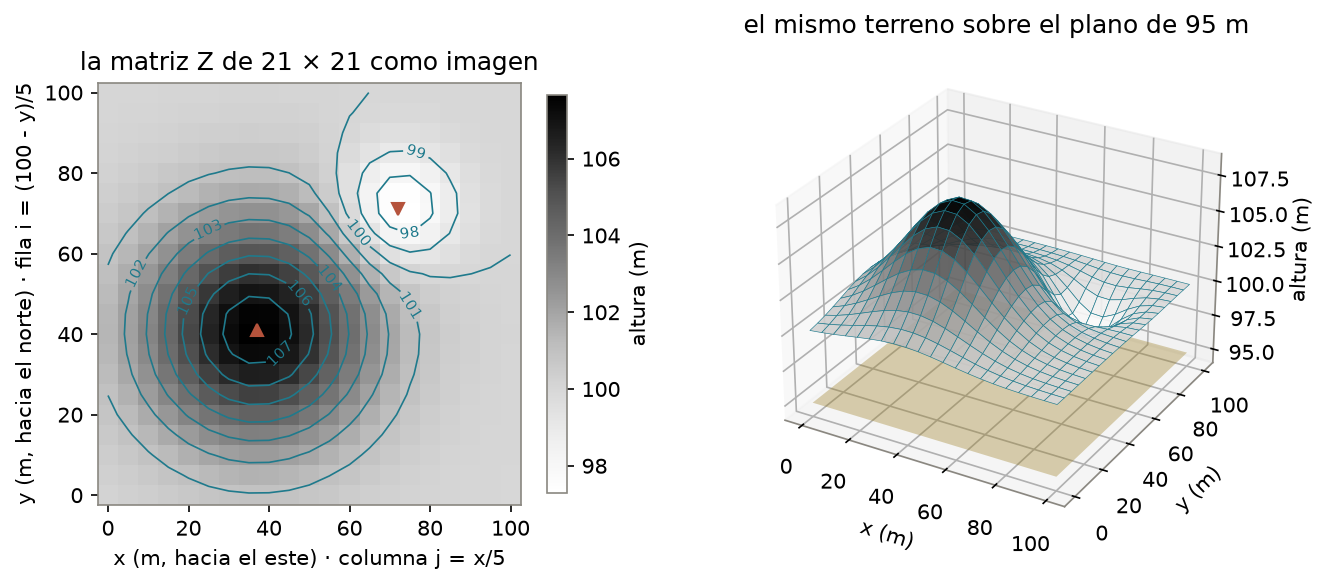
\includegraphics[width=\textwidth]{figuras/terreno-matriz/terreno_planilla.png}
\caption{El terreno de juguete. Izquierda: la matriz \(Z\) de \(21\times21\) pintada como una
foto en blanco y negro (más oscuro, más alto), con las líneas de igual altura cada \(1\) m; los
triángulos marcan el centro de la loma y el de la hondonada. Derecha: la misma matriz como
superficie, sobre el plano horizontal de \(95\) m de la aplicación. Generada con
\texttt{apunte/scripts/c3\_terreno\_matriz.py}.}
\label{fig:terreno-planilla}
\end{figure}

Las líneas de la figura~\ref{fig:terreno-planilla} unen puntos de igual altura; en los planos se
llaman \emph{curvas de nivel} y en \enquote{En profundidad} vemos cómo se trazan a partir de la
matriz. Donde las líneas se aprietan el terreno es empinado; donde se separan, es suave.

Mirar el terreno como matriz no es solo una manera de guardarlo. Las operaciones de matrices
tienen lectura directa. Sumar a \(Z\) una matriz constante es subir o bajar todo el terreno sin
cambiarle la forma. Multiplicar \(Z-100\) por \(2\) y volver a sumar \(100\) es exagerar el
relieve al doble sobre el llano. Restar dos matrices de alturas del mismo lugar, tomadas en dos
fechas, da cuánto se rellenó o se excavó en cada nodo. Invertir el orden de las filas es
espejar el terreno de norte a sur. Y transponer \(Z\) es reflejarlo respecto de la diagonal que
une la esquina noroeste con la sureste: cambia filas por columnas.

\subsection{Pendiente y orientación por diferencias}\label{sec:terreno-pendiente}

Imaginá que estás parado en un nodo de la ladera. ¿Cuánto se inclina el suelo y hacia dónde
correría el agua? Si tuviéramos la fórmula de la altura, la respuesta la darían las dos
derivadas parciales, cuánto sube el terreno por cada metro hacia el este y por cada metro hacia
el norte, puestas en una fila: el gradiente \(\nabla h=(\partial_xh\ \ \partial_yh)\), que el
capítulo~\ref{cap:derivada} estudia en detalle y que la sección~\ref{sec:gradiente-forma} ya
presentó como forma lineal. Pero en la matriz no hay fórmula: hay números en nodos separados
\(5\) m. Hacemos lo de la escalera de \enquote{La idea}: comparamos el vecino de adelante con el
de atrás y dividimos por lo que avanzamos entre los dos, \(2\Delta\). Esas cuentas se llaman
\emph{diferencias centradas}:
\[
  \partial_xh\approx\frac{z_{i,j+1}-z_{i,j-1}}{2\Delta},\qquad
  \partial_yh\approx\frac{z_{i-1,j}-z_{i+1,j}}{2\Delta}.
\]
En la segunda va primero la fila de arriba, \(i-1\), porque está al norte. Con el gradiente
aproximado salen dos números que interesan en el terreno. La \emph{pendiente} es cuánto se sube
por metro avanzado en la dirección más empinada, el largo \(\lVert\nabla h\rVert\); se da en
por ciento (metros que se suben cada \(100\) m) o como ángulo con la horizontal,
\(\arctan\lVert\nabla h\rVert\). La \emph{orientación} es hacia dónde mira la ladera, la
dirección en que baja más rápido, la del vector \(-\nabla h\) leído como flecha
\((-\partial_xh;\ -\partial_yh)\) (componente este, componente norte); la medimos como el
ángulo \(\mathrm{Az}\) que esa flecha forma con el norte, en sentido horario, como en la tabla
de notación del capítulo~0.

\begin{ejemplo}[Pendiente y orientación en un nodo]\label{ej:terreno-pendiente}
Tomamos el nodo de la fila \(10\) y la columna \(13\), en \(x=65\) m, \(y=50\) m, sobre el flanco
de la loma que mira a la hondonada. Su vecindario de \(3\times3\) en la matriz es
\[
  \begin{pmatrix}102{,}66&101{,}54&100{,}65\\103{,}41&\mathbf{102{,}33}&101{,}43\\103{,}84&102{,}74&101{,}82\end{pmatrix}\ \text{m}
\]
(fila de arriba, la del norte). Las diferencias centradas con \(\Delta=5\) m dan
\[
  \partial_xh\approx\frac{101{,}43-103{,}41}{10}=-0{,}198,\qquad
  \partial_yh\approx\frac{101{,}54-102{,}74}{10}=-0{,}120 .
\]
El terreno baja hacia el este y hacia el norte. La pendiente es
\(\sqrt{0{,}198^2+0{,}120^2}=0{,}2315\): \(23{,}15\) por ciento, o \(13{,}04^\circ\) con la
horizontal. La bajada apunta en la dirección \((0{,}198;\ 0{,}120)\), y su ángulo con el norte
es \(\arctan(0{,}198/0{,}120)=58{,}8^\circ\): la ladera mira al noreste, hacia la hondonada.

Como el terreno es de juguete, podemos comparar con la verdad. Derivando la fórmula de \(h\) en
\((65;\ 50)\) el gradiente exacto es \((-0{,}2027;\ -0{,}1186)\), con pendiente \(23{,}49\) por
ciento y orientación \(59{,}7^\circ\). Sin redondear las alturas a centímetros, las diferencias
centradas dan \((-0{,}1988;\ -0{,}1201)\) y \(23{,}22\) por ciento: el error en el gradiente es
de \(0{,}0043\). Si en lugar de los vecinos inmediatos usamos los que están a dos nodos
(paso efectivo de \(10\) m, la escalera de a cuatro escalones) el resultado empeora a
\((-0{,}1879;\ -0{,}1218)\), \(22{,}39\) por ciento y \(57{,}1^\circ\), con un error de
\(0{,}0152\): \(3{,}6\) veces más grande con el doble de paso. La
proposición~\ref{prop:terreno-centrada} de \enquote{En profundidad} explica por qué el error crece
como el cuadrado del paso, y por qué acá da \(3{,}6\) y no exactamente \(4\).
\end{ejemplo}

\begin{figure}[htbp]
\centering
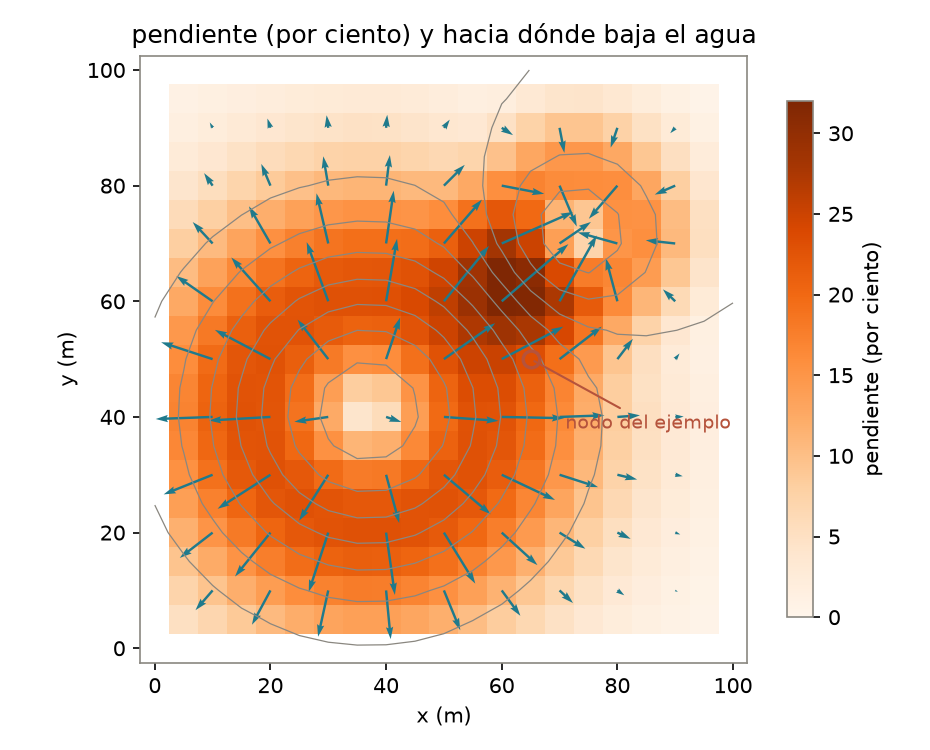
\includegraphics[width=.72\linewidth]{figuras/terreno-matriz/terreno_pendiente.png}
\caption{Pendiente del terreno de juguete calculada en cada nodo interior con diferencias
centradas (color, en por ciento) y la dirección de la bajada, \(-\nabla h\) (flechas, una de
cada dos nodos). El círculo marca el nodo del ejemplo~\ref{ej:terreno-pendiente}. En la cima de la
loma y en el fondo de la hondonada la pendiente se anula y la orientación no está definida.}
\label{fig:terreno-pendiente}
\end{figure}

Cerca de la cima de la loma la pendiente se anula, las flechas se achican y la orientación
deja de tener sentido: un terreno horizontal no mira hacia ningún lado. Es el mismo caso que el
gradiente nulo de un punto crítico (sección~\ref{sec:hessiana}).

\unidadInteractiva{10_jacobiano_primera_forma}{Jacobiano y primera forma fundamental}{Verificá: elegí la superficie «la loma r = (u, v, 2·exp(−(u²+v²)/8))» y dejá el punto en «u del punto» \(=2\), «v del punto» \(=1\). La tercera fila de \(J\) es el gradiente de la altura, \((\partial_uh\ \ \partial_vh)\); comprobá que da unos \((-0{,}535;\ -0{,}268)\). Calculá a mano la diferencia centrada con paso \(0{,}25\), \((h(2{,}25;\,1)-h(1{,}75;\,1))/0{,}5=(0{,}9374-1{,}2036)/0{,}5=-0{,}5324\), y compará. Después llevá el punto a la cima \((0,0)\) y mirá qué pasa con esa fila.}

\subsection{Volumen: una suma de prismas}\label{sec:terreno-volumen}

Supongamos que hay que bajar todo el terreno hasta un plano horizontal. ¿Cuánta tierra sale?
Entre el plano y la superficie queda un sólido, y su volumen es la integral doble de la altura
sobre el plano, \(\iint (h-z_0)\,dx\,dy\), donde \(z_0\) es la altura del plano. Con la matriz
no hay integral que hacer, pero sí una suma. Cada celda de la cuadrícula, el cuadrado de lado
\(\Delta\) que tiene cuatro nodos en las esquinas, es la base de un prisma; le damos como altura
el promedio de las alturas de sus cuatro esquinas sobre el plano. El volumen es la suma de los
prismas:
\[
  V\approx\Delta^2\sum_{\text{celdas}}\Bigl(\frac{z_{\mathrm{NO}}+z_{\mathrm{NE}}+z_{\mathrm{SE}}+z_{\mathrm{SO}}}{4}-z_0\Bigr).
\]
Cada nodo interior es esquina de cuatro celdas y cada nodo del borde, de dos (o de una, si es
una esquina del cuadrado). Sumando celda por celda, cada nodo aparece con peso \(1\) en el
interior, \(\tfrac12\) en el borde y \(\tfrac14\) en las cuatro esquinas, por \(\Delta^2\). La
proposición~\ref{prop:terreno-prisma} muestra que esta suma es el volumen exacto de la superficie
que se obtiene completando cada celda con la mezcla de sus cuatro esquinas que vemos en la
sección~\ref{sec:terreno-remuestreo}.

\begin{ejemplo}[Volumen de una celda y de todo el terreno]\label{ej:terreno-volumen}
Sobre el plano \(z_0=95\) m, la celda entre las filas \(10\) y \(11\) y las columnas \(8\) y \(9\),
cerca de la cima, tiene esquinas \(106{,}88\) (noroeste), \(106{,}41\) (noreste), \(106{,}96\)
(sureste) y \(107{,}46\) m (suroeste). Su promedio es \(106{,}93\) m, \(11{,}93\) m sobre el plano, y
el prisma tiene \(25\cdot11{,}9275=298{,}19\) m\(^3\).

Sumando los \(20\cdot20=400\) prismas de la cuadrícula se obtienen \(66\,218{,}9\) m\(^3\): una
capa de \(6{,}622\) m de espesor medio sobre los \(10\,000\) m\(^2\). Como la loma y la hondonada son
exponenciales de cuadrados, la integral de la fórmula se puede hacer exacta (cada exponencial se
separa en un factor que depende de \(x\) y otro de \(y\), y cada uno se integra con la función
error, \(\operatorname{erf}\)) y da \(66\,242{,}4\) m\(^3\). La suma de prismas se queda corta por
\(23{,}5\) m\(^3\), menos de cuatro diezmilésimos del total.

Un error frecuente es tomar cada nodo como una columna de \(5\times5\) m y sumar las \(441\)
columnas: da \(71\,641\) m\(^3\), un \(8{,}15\) por ciento de más. Las columnas de los nodos del borde
se salen del cuadrado: es como medir un terreno de \(105\) por \(105\) m. Los pesos \(\tfrac12\) y
\(\tfrac14\) del borde y de las esquinas corrigen eso.
\end{ejemplo}

\subsection{Remuestrear: pasar las alturas a otra cuadrícula}\label{sec:terreno-remuestreo}

¿Qué altura le damos a un punto que no es nodo? La pregunta aparece cada vez que hay que
entregar el terreno en otra cuadrícula, más gruesa, más fina o corrida, y a esa operación se la
llama \emph{remuestreo}. Las dos respuestas de \enquote{La idea} tienen nombre. La primera,
copiar la altura del nodo más cercano, es el \emph{vecino más próximo}: es rápida y no inventa
valores, pero el resultado es una superficie en escalones, con saltos donde cambia el nodo más
cercano. La segunda mezcla los cuatro nodos de la celda que contiene al punto. Si ponemos
coordenadas locales \((s,t)\in[0,1]^2\) en la celda (\(s\) hacia el este y \(t\) hacia el norte, en
unidades de paso) y llamamos \(f_{00}\), \(f_{10}\), \(f_{01}\), \(f_{11}\) a las alturas de las
esquinas suroeste, sureste, noroeste y noreste,
\[
  f(s,t)=(1-s)(1-t)\,f_{00}+s(1-t)\,f_{10}+(1-s)\,t\,f_{01}+s\,t\,f_{11}.
\]
Cada esquina pesa más cuanto más cerca está el punto, los cuatro pesos suman \(1\) y en cada
esquina \(f\) devuelve la altura medida. Es lineal a lo largo de cada recta paralela a los
lados de la celda (de ahí el nombre, \emph{bilineal}) pero no es un plano: tiene un término en
\(st\) que la tuerce. Es la misma función que usamos en \enquote{En profundidad} para trazar las
curvas de nivel dentro de una celda.

Cuál se equivoca menos depende del terreno, y lo medimos en la aplicación que sigue.

\subsection{Aplicación: un terreno de juguete y el volumen de un desmonte}\label{sec:terreno-aplicacion}

Antes de construir sobre un terreno con lomas hay que dejarlo horizontal. Si la plataforma
queda por debajo del terreno, hay que sacar la tierra que sobra por encima de ella: eso se
llama \emph{desmonte}. Para presupuestar la obra hace falta saber cuánta tierra es (cuántos
metros cúbicos), dónde el terreno es más empinado (ahí la máquina trabaja peor y el agua de
lluvia corre más rápido) y qué se pierde si los datos se entregan en una cuadrícula más gruesa.
Las tres preguntas se contestan con la matriz de alturas.

Los datos son los del terreno de juguete: el cuadrado de \(100\) por \(100\) m, la matriz \(Z\) de
\(21\times21\) nodos cada \(5\) m y la plataforma a \(z_0=95\) m. El punto más bajo del terreno
está a \(97{,}30\) m, así que todo el cuadrado queda por encima del plano y todo es desmonte.

\paragraph{Cuánta tierra.} La suma de prismas del ejemplo~\ref{ej:terreno-volumen} da
\(66\,218{,}9\) m\(^3\) contra \(66\,242{,}4\) m\(^3\) de la integral exacta: con un paso de \(5\) m
la matriz alcanza para el presupuesto.

\paragraph{Dónde es empinado.} Las diferencias centradas en los \(19\times19\) nodos interiores
(figura~\ref{fig:terreno-pendiente}) dan una pendiente media de \(13{,}29\) por ciento y una máxima de
\(31{,}99\) por ciento en el nodo de la fila \(7\) y la columna \(12\) (\(x=60\) m, \(y=65\) m), en el
cuello entre la loma y la hondonada, donde las dos laderas se suman. Calculada con la fórmula
en los mismos nodos, la máxima es \(33{,}58\) por ciento: las diferencias centradas con paso de
\(5\) m suavizan un poco las zonas más empinadas.

\paragraph{Qué se pierde con otra cuadrícula.} Supongamos que nos piden el terreno en una
cuadrícula de \(10\) m cuyo primer nodo está en \((3;\ 3)\), corrida \(3\) m al este y \(3\) m al
norte respecto de la nuestra: \(10\times10\) nodos, de \(x=3\) a \(x=93\) m y lo mismo en \(y\).
Ningún nodo nuevo coincide con uno viejo, así que hay que remuestrear. Como tenemos la fórmula,
podemos medir el error de cada método nodo por nodo:

{\small
\begin{center}
\begin{tabular}{l rrr}
\toprule
& error RMS (m) & error máximo (m) & volumen sobre \(95\) m en \([3,93]^2\) (m\(^3\))\\
\midrule
vecino más próximo & \(0{,}319\) & \(0{,}959\) & \(55\,882\) \ (\(-0{,}77\) por ciento)\\
bilineal & \(0{,}039\) & \(0{,}197\) & \(56\,178\) \ (\(-0{,}25\) por ciento)\\
alturas de la fórmula & \(0\) & \(0\) & \(56\,213\) \ (\(-0{,}18\) por ciento)\\
integral exacta & & & \(56\,317\)\\
\bottomrule
\end{tabular}
\end{center}
}

El error RMS es la raíz del promedio de los errores al cuadrado, un error típico. El vecino más
próximo se equivoca ocho veces más que la bilineal, y la figura~\ref{fig:terreno-remuestreo} muestra
por qué: cada nodo nuevo toma la altura del nodo viejo que está \(2\) m al este y \(2\) m al norte,
de modo que todo el terreno queda corrido \(2{,}83\) m hacia el suroeste. Donde la pendiente es
fuerte, un corrimiento horizontal se convierte en un error de altura (con \(32\) por ciento de
pendiente, \(2{,}83\) m de corrimiento pueden ser hasta unos \(0{,}9\) m), y su signo depende de hacia dónde
mira la ladera: las manchas rojas y azules de la figura son las dos caras de la loma. La bilineal
no corre el terreno; solo lo aplana un poco dentro de cada celda, y se equivoca en centímetros.

La última fila separa los dos errores del volumen. Aun con las alturas exactas en los nodos
nuevos, la cuadrícula de \(10\) m se queda corta por \(104\) m\(^3\): es lo que pierde la suma de prismas
con celdas más grandes. La bilineal agrega solo \(35\) m\(^3\) más de error; el vecino, \(331\) m\(^3\). Y
la pendiente máxima, calculada con diferencias centradas sobre la cuadrícula de \(10\) m remuestreada
con la bilineal, baja a \(26{,}70\) por ciento: con el doble de paso la ladera más empinada se ve
más suave de lo que es.

\begin{figure}[htbp]
\centering
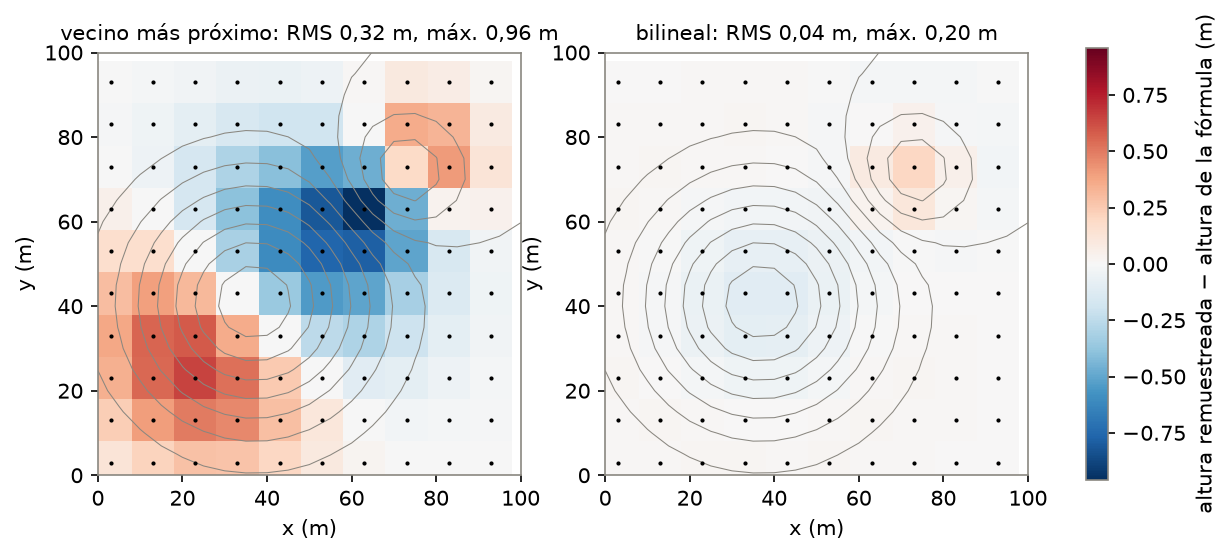
\includegraphics[width=\textwidth]{figuras/terreno-matriz/terreno_remuestreo.png}
\caption{Error de remuestrear el terreno de juguete a una cuadrícula de \(10\) m con origen en
\((3;\ 3)\) (puntos negros): altura remuestreada menos altura de la fórmula, con la misma escala de
color en los dos paneles. Izquierda, vecino más próximo; derecha, bilineal. En gris, las líneas de
igual altura cada \(1\) m.}
\label{fig:terreno-remuestreo}
\end{figure}

\begin{atencion}[Remuestrear no agrega información]
Pasar a una cuadrícula más gruesa pierde detalle que no se recupera: si después se vuelve a la
de \(5\) m, las alturas nuevas son mezclas de las de \(10\) m. Y el vecino más próximo, aunque no
invente valores, corre el terreno hasta medio paso: para alturas conviene la bilineal, y el
vecino solo cuando los valores son categorías (tipo de suelo, uso del terreno) que no se pueden
promediar.
\end{atencion}

\section{En profundidad}

\subsection{Por qué funcionan las cuentas de la cuadrícula}\label{sec:terreno-demostraciones}

Las dos cuentas de la sección anterior, la diferencia centrada y la suma de prismas, tienen una
justificación corta. La primera se apoya en el desarrollo de Taylor de una función de una
variable; la segunda, en integrar un polinomio en un cuadrado.

\begin{proposicion}[Error de la diferencia centrada]\label{prop:terreno-centrada}
Sea \(f\) una función con derivada tercera continua en \([x-k,\,x+k]\) y sea \(M\) un número mayor o igual
que \(\lvert f'''\rvert\) en todo ese intervalo. Entonces
\[
  \Bigl\lvert\frac{f(x+k)-f(x-k)}{2k}-f'(x)\Bigr\rvert\le\frac{M}{6}\,k^2 .
\]
\end{proposicion}

\begin{demostracion}
Por el desarrollo de Taylor con resto de Lagrange hasta el orden tres, existen \(\xi_+\in(x,x+k)\)
y \(\xi_-\in(x-k,x)\) tales que
\[
  f(x+k)=f(x)+f'(x)\,k+\tfrac12f''(x)\,k^2+\tfrac16f'''(\xi_+)\,k^3,\qquad
  f(x-k)=f(x)-f'(x)\,k+\tfrac12f''(x)\,k^2-\tfrac16f'''(\xi_-)\,k^3 .
\]
Restando, los términos en \(f(x)\) y en \(f''(x)\) se cancelan:
\(f(x+k)-f(x-k)=2f'(x)\,k+\tfrac16\bigl(f'''(\xi_+)+f'''(\xi_-)\bigr)k^3\). Dividiendo por \(2k\),
\[
  \frac{f(x+k)-f(x-k)}{2k}-f'(x)=\frac{f'''(\xi_+)+f'''(\xi_-)}{12}\,k^2 ,
\]
y el valor absoluto del numerador es a lo sumo \(2M\), lo que da la desigualdad.
\end{demostracion}

Para la derivada parcial \(\partial_xh\) se aplica a \(f(x)=h(x,y_i)\) con \(y\) fijo, y lo mismo
para \(\partial_yh\). La diferencia de un solo lado, \((f(x+k)-f(x))/k\), tiene en cambio un error
\(\tfrac12f''(x)\,k\) más términos de orden \(k^2\): es de primer orden, y por eso la tercera cuenta
de la escalera era la que menos se equivocaba. La desigualdad dice que el error es a lo sumo
proporcional a \(k^2\), y la fórmula de la demostración dice más: cuando \(k\) es chico, \(\xi_\pm\)
están cerca de \(x\) y el error se parece a \(\tfrac16f'''(x)\,k^2\), de modo que duplicar el paso
lo multiplica por casi \(4\). En el ejemplo~\ref{ej:terreno-pendiente} la razón fue \(3{,}6\): con
\(k=10\) m sobre una loma cuyo ancho característico es de unos \(20\) m, \(f'''\) ya cambia bastante
entre \(x\) y \(x\pm k\), y la aproximación \(f'''(\xi_\pm)\approx f'''(x)\) es gruesa.

\begin{proposicion}[La suma de prismas integra la bilineal]\label{prop:terreno-prisma}
Si \(f\) es la interpolación bilineal de los valores \(f_{00}\), \(f_{10}\), \(f_{01}\), \(f_{11}\) en
las esquinas de una celda cuadrada de lado \(\Delta\), entonces
\[
  \iint_{\text{celda}}f\,dA=\Delta^2\,\frac{f_{00}+f_{10}+f_{01}+f_{11}}{4}.
\]
En consecuencia, la suma de prismas de la sección~\ref{sec:terreno-volumen} es la integral exacta de
la superficie que completa cada celda con su bilineal.
\end{proposicion}

\begin{demostracion}
Con las coordenadas locales \(s=(x-x_0)/\Delta\), \(t=(y-y_0)/\Delta\), donde \((x_0,y_0)\) es la
esquina suroeste, se tiene \(dA=\Delta^2\,ds\,dt\). Desarrollando los productos de la fórmula de
la bilineal, \(f(s,t)=a+b\,s+c\,t+d\,st\) con
\[
  a=f_{00},\quad b=f_{10}-f_{00},\quad c=f_{01}-f_{00},\quad d=f_{00}-f_{10}-f_{01}+f_{11}.
\]
Como \(\int_0^1\!\int_0^1 ds\,dt=1\), \(\int_0^1\!\int_0^1 s\,ds\,dt=\int_0^1\!\int_0^1 t\,ds\,dt=\tfrac12\) y
\(\int_0^1\!\int_0^1 st\,ds\,dt=\tfrac14\),
\[
  \iint_{\text{celda}}f\,dA=\Delta^2\Bigl(a+\frac b2+\frac c2+\frac d4\Bigr).
\]
Reemplazando \(a\), \(b\), \(c\) y \(d\), el paréntesis vale
\(f_{00}\bigl(1-\tfrac12-\tfrac12+\tfrac14\bigr)+f_{10}\bigl(\tfrac12-\tfrac14\bigr)+f_{01}\bigl(\tfrac12-\tfrac14\bigr)+\tfrac14f_{11}
=\tfrac14\bigl(f_{00}+f_{10}+f_{01}+f_{11}\bigr)\). La segunda afirmación sale de sumar sobre las
celdas, porque la superficie bilineal por celdas es continua y la integral sobre el cuadrado es
la suma de las integrales sobre las celdas.
\end{demostracion}

Hecho geométrico: el prisma con la altura promedio de las cuatro esquinas tiene el mismo volumen
que el sólido de tapa torcida que forma la bilineal; lo que la tapa sube en un par de esquinas
opuestas lo baja en el otro, y el término en \(st\), que la tuerce, aporta lo mismo que si fuera
plano. Por eso el error de la suma de prismas no está en la suma: está en haber reemplazado el
terreno por la bilineal, y ese reemplazo mejora cuando la cuadrícula se afina. En el terreno de
juguete, con paso de \(5\) m el error fue de \(23{,}5\) m\(^3\) sobre \(66\,242\) m\(^3\), y con paso de
\(10\) m (y alturas exactas en los nodos) de \(104\) m\(^3\) sobre \(56\,317\) m\(^3\), en un cuadrado algo
menor. La celda de las curvas de nivel de más abajo da una comprobación: allí
\(f(s,t)=1496+8s+2t+2st\), su integral en la celda es \(1496+4+1+\tfrac12=1501{,}5\), y el promedio de
\(1496\), \(1504\), \(1508\) y \(1498\) es \(1501{,}5\).

\subsection{La SVD de un terreno real: del modelo digital de elevación a las curvas de nivel}\label{sec:svd-dem}
Un modelo digital de elevación es una
matriz: cada celda es una altura. El recorte de \(512\times512\) celdas del Copernicus DEM
GLO-30 sobre la Precordillera de Mendoza (\file{datos/dem\_copernicus/}, latitud
\(-32{,}284\) a \(-32{,}142\), longitud \(-69{,}000\) a \(-68{,}858\), una celda
\(\approx30\) m) tiene alturas entre \(1014\) y \(2989\) m, con desvío \(406\) m. Como
matriz tiene \(512\) valores singulares, ordenados de mayor a menor, y quedarse con los
\(k\) primeros términos \(\sigma_iu_iv_i^T\) es la mejor aproximación de rango \(k\): el
mismo problema 4 de la sección~\ref{cap:cuatro-problemas}, en grande. Los valores salieron
de \file{svd\_dem\_proto.py}, corrido fuera del navegador (la SVD completa tarda
\(0{,}06\) s en un M1):

{\small
\begin{center}
\begin{tabular}{l rrrrrrr}
\toprule
\(k\) (términos) & 1 & 2 & 5 & 10 & 20 & 50 & 100\\
\midrule
error RMS (m) & 103 & 66 & 31 & 17 & 9{,}8 & 4{,}4 & 2{,}0\\
\bottomrule
\end{tabular}
\end{center}
}

Hecho geométrico: una matriz constante es de rango \(1\), y la altura media del recorte
(unos \(1600\) m) es la \enquote{meseta} sobre la que está apoyado el relieve. Por eso
\(\sigma_1\) domina y la energía acumulada \(\sum_{i\le k}\sigma_i^2/\sum\sigma_i^2\) ya
da \(99{,}6\)\,\% con \(k=1\): esa cifra engaña, mide la meseta y no el relieve. El RMS
del error, o restar la media antes de descomponer (lo mismo que centrar la nube de puntos
en el problema 4), muestra lo que importa: el relieve \enquote{aparece} alrededor de \(k=20\)
(error de \(9{,}8\) m sobre un terreno de casi \(2000\) m de desnivel, la diferencia de altura entre su punto más bajo y el más alto) y con \(100\)
términos de \(512\) el error es de \(2\) m. La unidad \texttt{09\_cambio\_de\_base\_svd}
(apéndice~\ref{ap:notebooks}) carga ese mismo recorte y deja mover \(k\) en vivo.

\unidadInteractiva{09_cambio_de_base_svd}{Cambio de base y SVD}{Explorá: en la parte del recorte de la Precordillera, mové «k (valores singulares que conservamos)» de \(1\) a \(50\) y mirá cuándo aparecen los cerros chicos del centro. Comprobá que con \(k=20\) el error RMS de la submuestra de \(128\times128\) es de unos \(9{,}8\) m, el de la tabla de arriba.}

% --- 09-svd-nivel3 (redactado 2026-10-18) ---

Este complemento extiende la lectura de la SVD al terreno con el mismo recorte de Copernicus que usa la unidad \texttt{09\_cambio\_de\_base\_svd}. Todos los números salen de \texttt{np.linalg.svd} sobre la matriz de \(512\times512\) (\file{apunte/figuras/svd/gen\_dem\_curvas\_nivel.py}).

\subsubsection{El modelo digital de elevación como matriz y como función}

Como vimos en la sección~\ref{sec:terreno-planilla}, un modelo digital de elevación es una tabla
de alturas tomadas sobre una cuadrícula regular. En el recorte de la Precordillera, la fila \(i\) corresponde a una latitud (de norte
a sur, desde \(-32{,}142^\circ\) hasta \(-32{,}284^\circ\)), la columna \(j\) a una longitud
(de oeste a este, desde \(-69{,}000^\circ\) hasta \(-68{,}858^\circ\)) y la entrada
\(z_{ij}\) es la altura en metros. El paso de la cuadrícula es de un segundo de arco en las dos
direcciones; sobre el elipsoide de referencia del capítulo~\ref{cap:elipsoide}, a la latitud media del recorte, un segundo de latitud
mide \(30{,}80\) m y un segundo de longitud \(26{,}19\) m. El recorte cubre
\(15{,}8\) km de norte a sur por \(13{,}4\) km de este a oeste, con alturas entre
\(1014\) y \(2989\) m, media \(1626\) m y desvío \(406\) m.

La misma tabla admite dos lecturas, y las dos nos sirven.

\begin{itemize}
  \item \textbf{Como matriz} \(Z\in\R^{512\times512}\). Cada fila es un perfil
  oeste--este del terreno a latitud fija; cada columna, un perfil norte--sur a longitud fija.
  Sumar matrices es sumar relieves; multiplicar por un número es exagerar o aplanar el
  relieve.
  \item \textbf{Como muestra de una función} \(z=f(x,y)\) definida en todo el rectángulo,
  de la que solo conocemos los valores en los nodos: \(z_{ij}=f(x_j,y_i)\). La cuadrícula es
  la regla con que leemos el terreno, en el sentido de la
  sección~\ref{sec:puntos-formas-grillas}: los números \((i,j)\) no son metros sino marcas
  de dos mazos de rectas, uno de meridianos y otro de paralelos.
\end{itemize}

La primera lectura es la que permite descomponer; la segunda, la que permite hablar de
gradiente, plano tangente y curvas de nivel. Lo que sigue va y viene entre las dos.

\subsubsection{La SVD del terreno: una suma de relieves separables}\label{sec:svd-dem-separables}

Como cualquier matriz, \(Z\) se escribe
\[
  Z=U\Sigma V^T=\sum_{i=1}^{512}\sigma_i\,u_i\,v_i^T ,
  \qquad \sigma_1\ge\sigma_2\ge\dots\ge\sigma_{512}\ge0 .
\]
Cada término \(\sigma_iu_iv_i^T\) es una matriz de rango uno, y una matriz de rango uno
tiene una forma muy particular: su entrada \((r,c)\) es \(\sigma_i\,(u_i)_r\,(v_i)_c\), el
producto de un número que depende solo de la fila por otro que depende solo de la columna.

\paragraph{Hecho geométrico: el relieve separable.} Un término de rango uno es un relieve
que se obtiene tomando un perfil norte--sur \(u_i\) y un perfil oeste--este \(v_i\) y
multiplicándolos punto a punto. Todos sus perfiles oeste--este tienen la misma forma
\(v_i\), escalada por el valor de \(u_i\) en esa latitud; todos sus perfiles norte--sur tienen
la forma \(u_i\). Escalera: en \(\R\), un número es un relieve de una sola celda; en
\(\R^2\), una matriz de rango uno es un terreno \enquote{tejido} con un solo hilo en cada
dirección; la SVD dice que cualquier terreno es una suma de esos tejidos, ordenados por
importancia. Los vectores \(u_i\) y \(v_i\) son unitarios y adimensionales, de modo que
\(\sigma_i\) lleva las unidades de la altura: es la \enquote{amplitud} del tejido \(i\).

Los cinco primeros valores singulares del recorte son
\[
  \sigma_1=856\,621\ \text{m},\quad
  \sigma_2=40\,405\ \text{m},\quad
  \sigma_3=22\,048\ \text{m},\quad
  \sigma_4=18\,308\ \text{m},\quad
  \sigma_5=8\,784\ \text{m},
\]
y siguen bajando: \(\sigma_{20}=1467\) m, \(\sigma_{50}=453\) m, \(\sigma_{100}=170\) m. El
primero es más de veinte veces el segundo. La razón está en la meseta del remate: si \(Z\) fuera
constante e igual a la media \(\bar z\), sería \(\bar z\) por la matriz de unos, de rango uno,
con \(\sigma_1=\bar z\cdot512\) y \(u_1=v_1=\tfrac1{\sqrt{512}}(1,\dots,1)\). En el
recorte real \(\sigma_1/(\bar z\cdot512)=1{,}029\), y las entradas de \(u_1\) van de
\(0{,}0406\) a \(0{,}0461\), alrededor de \(1/\sqrt{512}=0{,}0442\): el perfil norte--sur del
primer término es casi plano. Las de \(v_1\) van de \(0{,}0302\) a \(0{,}0678\): el perfil
oeste--este baja a menos de la mitad, como el terreno, cuya altura media por columna pasa de
\(2563\) m en el borde oeste a \(1141\) m en el borde este. El primer término es entonces una
meseta inclinada hacia el este, con alturas entre \(1048\) y \(2677\) m.

\paragraph{Cuánto explica cada término.} Truncar la suma en \(k\) términos da
\(Z_k=\sum_{i\le k}\sigma_iu_iv_i^T\), la mejor aproximación de rango \(k\) de \(Z\): ninguna
otra matriz de rango \(k\) queda más cerca en la norma de Frobenius, la raíz de la suma de los
cuadrados de las entradas (es el problema 4 de la sección~\ref{cap:cuatro-problemas}). Como
las columnas de \(U\) y de \(V\) son ortonormales, los términos son perpendiculares entre sí
como matrices, y Pitágoras da
\[
  \|Z\|_F^2=\sum_{i}\sigma_i^2,\qquad
  \|Z-Z_k\|_F^2=\sum_{i>k}\sigma_i^2,\qquad
  \mathrm{RMS}_k=\sqrt{\frac{1}{512^2}\sum_{i>k}\sigma_i^2}\ .
\]
El error medio cuadrático en metros se lee directamente de los valores singulares que
descartamos, sin reconstruir nada. Comprobación con una matriz de juguete:
\(Z=\begin{pmatrix}12&11\\11&12\end{pmatrix}\) m, simétrica, con autovalores \(23\) y \(1\)
y autovectores \((1,1)\) y \((1,-1)\); sus valores singulares son \(23\) y \(1\), y
\(Z_1=23\cdot\tfrac12\begin{pmatrix}1&1\\1&1\end{pmatrix}\) es la meseta de \(11{,}5\) m. El
error \(Z-Z_1\) vale \(\pm0{,}5\) m en las cuatro celdas, su RMS es \(0{,}5\) m, y la fórmula
da \(\sqrt{1^2/4}=0{,}5\) m.

Para el recorte, con \(\|Z\|_F=858\,240\) m:

{\small
\begin{center}
\begin{tabular}{l rrrr}
\toprule
\(k\) & 1 & 5 & 10 & 20\\
\midrule
energía \(\sum_{i\le k}\sigma_i^2/\sum_i\sigma_i^2\) & \(99{,}62\)\,\% & \(99{,}967\)\,\% & \(99{,}990\)\,\% & \(99{,}997\)\,\%\\
error relativo \(\|Z-Z_k\|_F/\|Z\|_F\) & \(6{,}14\)\,\% & \(1{,}82\)\,\% & \(1{,}01\)\,\% & \(0{,}59\)\,\%\\
error RMS (m) & \(102{,}9\) & \(30{,}6\) & \(16{,}9\) & \(9{,}8\)\\
error máximo en una celda (m) & \(641\) & \(236\) & \(126\) & \(75\)\\
\bottomrule
\end{tabular}
\end{center}
}

Los RMS coinciden con los de la tabla del remate y con los que imprime la unidad
\texttt{09} con el repositorio clonado; en el navegador la unidad usa la submuestra de
\(128\times128\) (una celda de cada cuatro) y da \(103{,}5\), \(30{,}8\), \(17{,}0\) y
\(9{,}8\) m para los mismos \(k\). La primera fila muestra otra vez que la energía engaña: con
un solo término ya pasa del \(99{,}6\)\,\%, y sin embargo ese término se equivoca en \(103\) m
de RMS y en \(641\) m en la peor celda. Restando la media antes de descomponer, el primer
término deja de pagar la meseta y el RMS de \(k=1\) baja a \(85{,}4\) m; desde \(k\approx20\)
las dos versiones dan lo mismo. Para dibujar curvas de nivel la fila que importa es la del
RMS, porque se mide en las mismas unidades que la equidistancia.

\subsubsection{Curvas de nivel en una cuadrícula}\label{sec:svd-dem-curvas}

\paragraph{Definición.} La curva de nivel \(c\) de \(z=f(x,y)\) es el conjunto de los puntos
del plano donde \(f(x,y)=c\): la huella, proyectada sobre el plano horizontal, del corte del
terreno con el plano \(z=c\). En un plano topográfico se dibujan las curvas de una familia
equiespaciada, \(c=c_0+n\,e\), donde \(e\) es la \emph{equidistancia}; cada quinta curva es
maestra y lleva rotulada su altura.

\paragraph{Hecho geométrico: la curva de nivel es la recta de nivel cero del plano
tangente.} Cerca de un punto \(p\), el terreno se parece a su plano tangente,
\(f(p+h)\approx f(p)+df_p(h)\), donde \(df_p\) es la forma lineal que toma un desplazamiento
horizontal \(h\) y devuelve cuánto sube el terreno. Sus rectas de nivel son un mazo de
paralelas equiespaciadas, una regla graduada tirada sobre el plano
(sección~\ref{sec:puntos-formas-grillas}). Moverse a lo largo de la curva de nivel es moverse
sin subir ni bajar, es decir, en una dirección \(h\) con \(df_p(h)=0\): la tangente a la curva
de nivel es la recta de nivel cero de la forma \(df_p\), el núcleo de esa forma. Esta
afirmación no usa ninguna métrica. La que sí la usa es la otra, \enquote{el gradiente es perpendicular
a la curva de nivel}: para hablar de la dirección de máxima pendiente hay que convertir la
forma en un vector con el producto interno, y en la cuadrícula del recorte ese producto interno no es
el de los índices (secciones~\ref{sec:puntos-formas-grillas} y~\ref{cap:curvatura}). La
escalera: en \(\R\), la \enquote{curva} de nivel de \(z=f(x)\) es un punto aislado donde
\(f(x)=c\); en \(\R^2\), una curva; en \(\R^3\), las superficies de nivel de una función de
tres variables, como las superficies de igual temperatura o de igual potencial.

\paragraph{Una celda a mano.} En la cuadrícula solo tenemos alturas en los nodos. Dentro de cada
celda, entre cuatro nodos vecinos, completamos \(f\) de la manera más simple que respete los
cuatro valores: lineal a lo largo de cada lado de la celda. Una curva de nivel cruza un lado
exactamente cuando sus dos extremos quedan uno por encima y otro por debajo de \(c\), y el
punto de cruce se obtiene por interpolación lineal, como una regla de tres. Tomemos una celda
con coordenadas locales \((s,t)\in[0,1]^2\) (\(s\) hacia el este, \(t\) hacia el norte, en
unidades de celda) y alturas
\[
  f(0,0)=1496,\quad f(1,0)=1504,\quad f(1,1)=1508,\quad f(0,1)=1498\ \text{m},
\]
y busquemos la curva de \(1500\) m. El lado sur va de \(1496\) a \(1504\): lo cruza en
\(s=\frac{1500-1496}{1504-1496}=0{,}5\). El lado norte va de \(1498\) a \(1508\): lo cruza en
\(s=\frac{1500-1498}{1508-1498}=0{,}2\). Los lados oeste (\(1496\), \(1498\)) y este
(\(1504\), \(1508\)) no tienen cambio de signo. El tramo de curva dentro de la celda es el
segmento de \((0{,}5;\ 0)\) a \((0{,}2;\ 1)\).

\begin{center}
\begin{tikzpicture}[scale=2.4]
  \fill[teallight!40] (0,0)--(0.5,0)--(0.2,1)--(0,1)--cycle;
  \draw[mainline] (0,0) rectangle (1,1);
  \draw[rust,line width=1.2pt] (0.5,0)--(0.2,1);
  \fill (0,0) circle (0.7pt) node[below left,font=\small] {\(1496\)};
  \fill (1,0) circle (0.7pt) node[below right,font=\small] {\(1504\)};
  \fill (1,1) circle (0.7pt) node[above right,font=\small] {\(1508\)};
  \fill (0,1) circle (0.7pt) node[above left,font=\small] {\(1498\)};
  \node[font=\small,text=rust] at (0.62,0.5) {\(1500\)};
  \node[font=\small,text=muted] at (0.12,0.5) {\(-\)};
  \node[font=\small,text=muted] at (0.85,0.5) {\(+\)};
  \node[font=\footnotesize,below] at (0.5,-0.02) {\(s=0{,}5\)};
  \node[font=\footnotesize,above] at (0.2,1.02) {\(s=0{,}2\)};
\end{tikzpicture}
\end{center}

Con cuatro nodos y dos estados para cada uno (por encima o por debajo de \(c\)) hay
\(2^4=16\) configuraciones, que se reducen a cuatro casos. Si los cuatro nodos están del mismo
lado, la curva no entra en la celda. Si uno solo difiere, la curva corta la esquina de ese
nodo con un segmento entre los dos lados que llegan a él. Si dos nodos vecinos están de un
lado y los otros dos del otro, como en la celda de recién, un segmento atraviesa la celda.
Y si los nodos de una diagonal están por encima y los de la otra por debajo, hay cuatro
cruces y dos maneras de unirlos de a pares; el caso se decide con el valor del centro de la
celda, el promedio de los cuatro nodos, que dice si las dos esquinas altas están conectadas
por un lomo o separadas por un collado. Recorrer la cuadrícula celda por celda aplicando estos
cuatro casos y empalmar los segmentos que comparten un punto de cruce es, en lo esencial, lo que
hace una rutina de curvas de nivel como \texttt{matplotlib.pyplot.contour}.

\paragraph{La misma celda, leída con el gradiente.} La función que vale lo que vale en los
cuatro nodos y es lineal a lo largo de cada recta paralela a los lados (la interpolación
bilineal) es
\(f(s,t)=1496+8s+2t+2st\) (se verifica en los cuatro vértices). En el centro de la celda,
\(\partial f/\partial s=8+2t=9\) y \(\partial f/\partial t=2+2s=3\) metros por celda: la
forma lineal \(df=(9\ \ 3)\), cuyo núcleo es la dirección \((-1,3)\). El segmento que
trazamos tiene dirección \((0{,}2-0{,}5;\ 1-0)=(-0{,}3;\ 1)\), proporcional a
\((-1;\ 3{,}33)\): casi la recta de nivel cero del plano tangente. No coinciden del todo
porque el término \(2st\) curva la curva de nivel dentro de la celda (es un arco de hipérbola
y el segmento es su cuerda); en el centro, la curva verdadera pasa por \(t=0{,}444\) cuando
\(s=0{,}35\) y el segmento por \(t=0{,}5\), una diferencia de \(0{,}06\) celdas, menos de
\(2\) m sobre el terreno.

Ahora la métrica. Pasada a metros, con \(26{,}19\) m por celda hacia el este y \(30{,}80\) m
hacia el norte, la forma es \(df=(9/26{,}19\ \ \ 3/30{,}80)=(0{,}344\ \ 0{,}097)\), sin
unidades (metros de subida por metro de avance), y la tangente a la curva de nivel, que es
la misma dirección física, se escribe \((-26{,}19;\ 92{,}40)\) m; el producto da \(-9+9=0\), como
debe ser, porque el núcleo de una forma no depende de cómo graduemos los ejes. La dirección de
máxima pendiente, en cambio, es \((0{,}344;\ 0{,}097)\) en metros, que forma con el este un
ángulo de \(15{,}8^\circ\); el \enquote{perpendicular} calculado con los índices, \((9,3)\) en celdas,
corresponde en metros a \((235{,}7;\ 92{,}4)\), a \(21{,}4^\circ\) del este. Los
\(5{,}6^\circ\) de diferencia son la métrica de la cuadrícula geográfica que se olvida.

\subsubsection{Curvas de nivel sobre \texorpdfstring{$Z_k$}{Zk}: filtrar el relieve con la SVD}\label{sec:svd-dem-filtro}

La rutina de curvas de nivel acepta cualquier matriz de alturas. Si en lugar de \(Z\) le damos
\(Z_k\), dibuja las curvas de un terreno simplificado que conserva los \(k\) tejidos de mayor
amplitud. La figura~\ref{fig:svd-dem-curvas} muestra el resultado con la misma equidistancia
de \(50\) m y maestras cada \(250\) m en los cuatro paneles.

\begin{figure}[htbp]
\centering
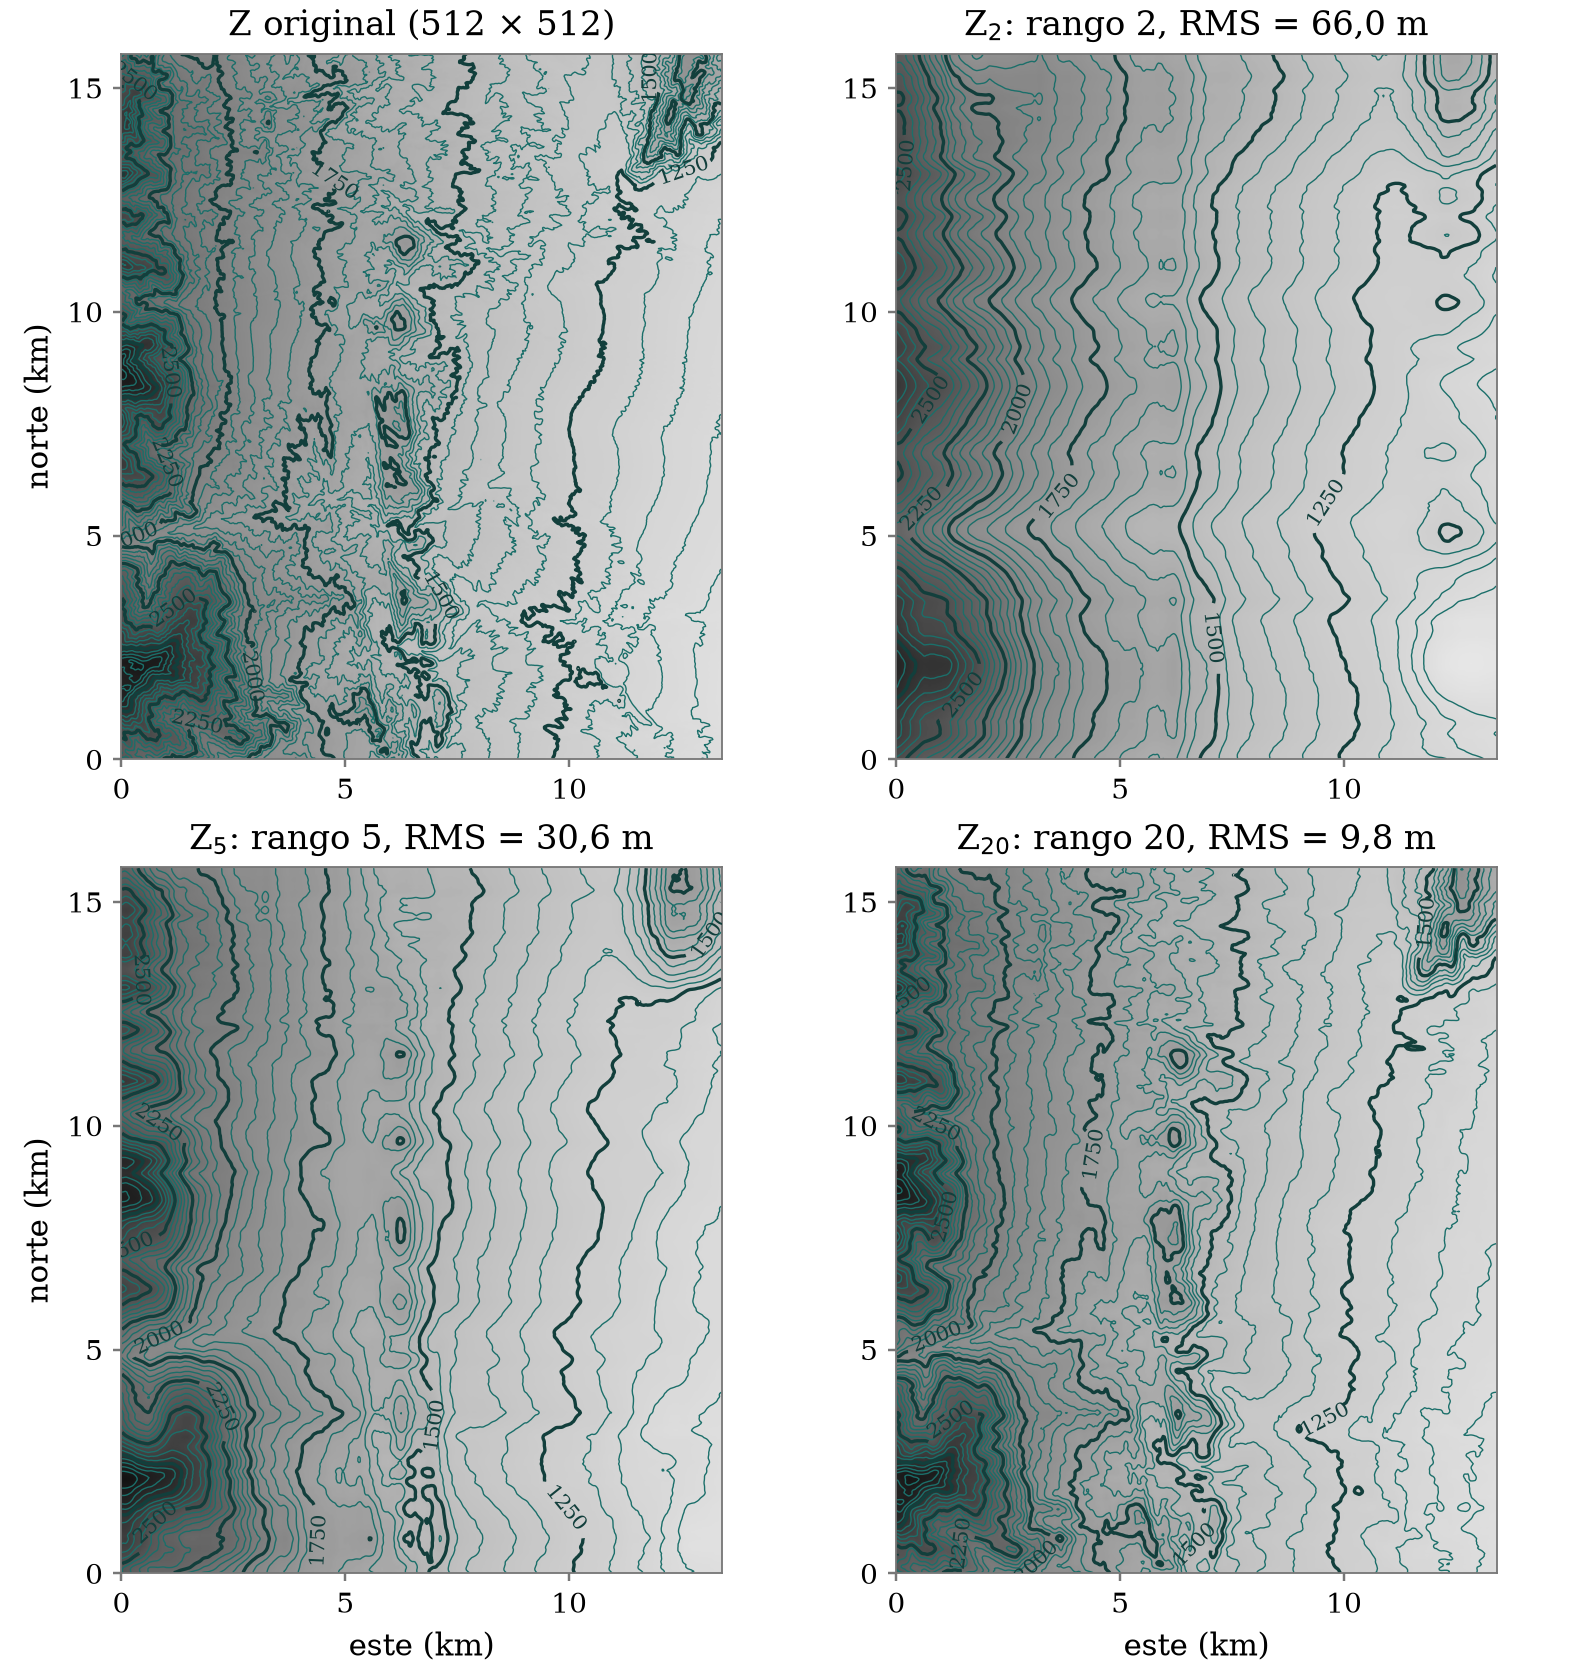
\includegraphics[width=\textwidth]{figuras/svd/dem_curvas_nivel.png}
\caption{Curvas de nivel del recorte de la Precordillera de Mendoza (Copernicus,
\(512\times512\) celdas de \(1''\)), equidistancia \(50\) m, maestras cada \(250\) m, trazadas
sobre la matriz original y sobre sus aproximaciones de rango \(2\), \(5\) y \(20\). El fondo gris
es la altura (más oscuro, más alto). Generada con
\texttt{apunte/figuras/svd/gen\_dem\_curvas\_nivel.py}. Datos: Copernicus DEM GLO-30, \enquote{\textcopyright{} DLR e.V. 2010-2014 and \textcopyright{} Airbus Defence and Space GmbH 2014-2018 provided under COPERNICUS by the European Union and ESA}.}
\label{fig:svd-dem-curvas}
\end{figure}

\paragraph{Lo que se ve.} Con \(k=2\) quedan las formas grandes: el cordón alto del oeste, el
descenso hacia el este y un par de lomas, todo con curvas de trazo largo y casi paralelas a
los meridianos. Es lo que cabe esperar de una suma de dos tejidos: cada uno tiene perfiles
norte--sur de una sola forma, de modo que las curvas tienden a alinearse con las columnas o con
las filas de la cuadrícula. Ese sesgo es propio del método, no del terreno: un cordón oblicuo a la
cuadrícula necesita muchos términos separables para quedar bien descripto. Con \(k=5\) aparecen
el cerro del ángulo noreste y los cerros del centro, todavía como manchas suaves. Con
\(k=20\) vuelve casi todo el dibujo: los cerros chicos alineados de norte a sur en el centro,
las entradas de las curvas en los cauces del oeste, los bordes quebrados de las maestras de
\(1500\) y \(1250\) m. Medido por el largo total de las curvas
de \(50\) m sobre el terreno, la matriz original tiene \(1174\) km de curvas repartidos en
\(307\) tramos; \(Z_{20}\) tiene \(923\) km en \(172\) tramos; \(Z_5\), \(716\) km en
\(119\); \(Z_2\), \(609\) km en \(83\). Cada término agregado agrega rugosidad, y una parte
de esa rugosidad es relieve y otra parte es ruido del propio modelo (es un modelo de superficie,
con vegetación y artefactos de medición, no de terreno desnudo).

\paragraph{Cuándo el filtro sirve y cuándo falsea.} Truncar la SVD es un filtro con una
ventaja clara: el error está controlado por números que conocemos antes de dibujar, los
\(\sigma_i\) descartados. Sirve cuando la escala del plano no puede mostrar el detalle: en
cartografía a escala chica, con equidistancia grande, las curvas de la matriz original salen
temblorosas y llenas de tramos cortos que el dibujante igual eliminaría a mano, y \(Z_k\) los
elimina con un criterio uniforme en toda la hoja. Falsea cuando lo que se busca es justamente
el detalle local: el talud de un camino, una cárcava, el borde de una terraza, el pie de un
cerro que define un límite. Un error RMS bajo es un promedio sobre \(262\,144\) celdas y no
garantiza nada en una celda en particular: con \(k=20\) el RMS es \(9{,}8\) m pero el error
llega a \(75\) m en la peor celda, aunque solo en el \(0{,}04\)\,\% de las celdas supera los
\(50\) m. Para un relevamiento de detalle, la matriz que manda es \(Z\), y conviene mirar
\(Z-Z_k\) como mapa para saber qué se está tirando.

\paragraph{Un criterio numérico para elegir \(k\).} Una curva de nivel está bien ubicada si
el error en altura es chico frente a la equidistancia: si el error vale la mitad de \(e\), la
curva puede confundirse con su vecina. Una regla práctica razonable es pedir
\[
  \mathrm{RMS}_k\le\frac{e}{5},
\]
y como \(\mathrm{RMS}_k\) se calcula solo con los \(\sigma_i\), el menor \(k\) que la cumple
se busca recorriendo la lista de valores singulares. En el recorte de la Precordillera:

{\small
\begin{center}
\begin{tabular}{r r r r r}
\toprule
equidistancia \(e\) & error admitido \(e/5\) & menor \(k\) & \(\mathrm{RMS}_k\) & error máximo\\
\midrule
\(100\) m & \(20\) m & \(9\) & \(18{,}7\) m & \(129\) m\\
\(50\) m & \(10\) m & \(20\) & \(9{,}8\) m & \(75\) m\\
\(25\) m & \(5\) m & \(44\) & \(4{,}95\) m & \(33\) m\\
\bottomrule
\end{tabular}
\end{center}
}

Para la equidistancia de la figura, \(50\) m, el criterio elige \(k=20\): veinte tejidos de
\(512\), y \(Z_{20}\) se guarda con \(20\cdot(512+512+1)=20\,500\) números en lugar de
\(262\,144\), menos del \(8\)\,\%. El error en altura se traduce en un corrimiento horizontal
de la curva que depende de la pendiente: donde el terreno sube \(\tan\theta\) metros por
metro, un error vertical \(\delta\) corre la curva unos \(\delta/\tan\theta\) metros. La
pendiente mediana del recorte es \(0{,}188\) (unos \(10{,}6^\circ\)), así que los \(9{,}8\) m
de \(Z_{20}\) mueven las curvas del orden de \(52\) m, dos celdas, en un terreno típico, y
bastante más en los llanos del este, donde la pendiente es menor. Es el mismo número visto de
otro modo: en escala \(1\!:\!50\,000\), \(52\) m son un milímetro del plano, el límite de lo
que se dibuja; en escala \(1\!:\!5000\) son un centímetro, y ahí \(k=20\) ya no alcanza.

\subsubsection{Conexiones con el resto del programa}\label{sec:svd-dem-conexiones}

\paragraph{El plano que mejor aproxima y la pseudoinversa.} El primer modelo de un terreno que se le
ocurre a un agrimensor no es \(Z_1\) sino un plano, \(z=a\,x+b\,y+c\), con \(x\) hacia el este
y \(y\) hacia el norte en metros. Ajustarlo es un sistema sobredeterminado de \(262\,144\)
ecuaciones con tres incógnitas, una por celda, \(a\,x_j+b\,y_i+c\approx z_{ij}\), que se
resuelve con la pseudoinversa de la sección~\ref{sec:pseudoinversa}: \((a,b,c)=A^{+}z\), con
\(A\) de \(262\,144\times3\) y columnas \(x\), \(y\) y unos. En el recorte da un plano que baja
\(97\) m por kilómetro hacia el este y sube \(4{,}4\) m por kilómetro hacia el norte
(pendiente de \(5{,}5^\circ\)), con un RMS de \(153{,}7\) m.

La comparación con la SVD es instructiva. El plano, escrito como matriz, es
\((b\,y_i+c)\cdot1+a\cdot x_j\): la suma de una matriz que solo depende de la fila y otra que
solo depende de la columna, de rango dos. Por lo tanto su error no puede ser menor que el de la
mejor aproximación de rango dos, y efectivamente \(153{,}7\ \text{m}>66{,}0\ \text{m}\). Lo
llamativo es que también pierde contra \(Z_1\), de rango uno, que da \(102{,}9\) m. La razón
es que el plano obliga a los perfiles a ser rectas, mientras que la SVD elige los perfiles que
mejor describen el terreno, y el perfil oeste--este real, que cae más de \(1400\) m en
\(13\) km de manera nada uniforme, no es una recta. Las dos aproximaciones son de mínimos cuadrados (minimizan la suma de los
cuadrados de las diferencias) con el mismo dibujo de la proyección ortogonal (caja \enquote{El dibujo único detrás de \(Ax\approx b\)}
de la sección~\ref{cap:cuatro-problemas}); lo que cambia es el subespacio sobre el que
proyectamos: planos en un caso, matrices de rango \(k\) en el otro.

\paragraph{La cuadrícula geográfica no es cuadrada.} Todo lo anterior trató a \(Z\) como una
tabla con celdas iguales, y la SVD lo hace sin preguntar: suma cuadrados de alturas celda por
celda. Pero las celdas de un segundo de arco no son cuadradas (\(30{,}80\) por \(26{,}19\) m
en este recorte) ni todas iguales: el ancho este--oeste es \(N\cos\varphi\) por un segundo
en radianes, con \(N\) la gran normal del elipsoide, y pasa de \(26{,}17\) m en el borde sur a
\(26{,}21\) m en el borde norte. En \(15\) km la variación es despreciable; en un modelo de elevación que cubre
varios grados de latitud no lo es, y una celda cerca del polo es una astilla. La cuadrícula
\((\lambda,\varphi)\) es una parametrización del elipsoide con primera forma fundamental
\(ds^2=N^2\cos^2\varphi\,d\lambda^2+M^2\,d\varphi^2\) (secciones~\ref{sec:metrica}
y~\ref{cap:elipsoide}). Para las curvas de nivel eso tiene dos consecuencias. El trazado
mismo no cambia, porque una curva de nivel es el núcleo de una forma y no necesita métrica.
Cambian todas las cuentas que miden: el largo de las curvas, las pendientes, la dirección de
máxima pendiente y el corrimiento horizontal de una curva por un error vertical, que en este
recorte hicimos convirtiendo celdas a metros con los dos factores de la métrica. Y si
quisiéramos que la propia SVD pesara cada celda por el área que representa, habría que
descomponer \(D_1^{1/2}\,Z\,D_2^{1/2}\), con \(D_1\) y \(D_2\) diagonales con los pesos de
filas y columnas: otra vez, la base privilegiada la elige la regla de medir.

\begin{resultado}[Lo que sabemos hacer con un modelo digital de elevación]
Leerlo como matriz \(Z\) y como muestra de una función \(z=f(x,y)\) en una cuadrícula geográfica.
Descomponerlo en tejidos separables \(\sigma_iu_iv_i^T\) y saber, solo con los \(\sigma_i\)
descartados, el error RMS en metros de la aproximación \(Z_k\). Trazar sus curvas de nivel
celda por celda por interpolación lineal, sabiendo que cada tramo aproxima la recta de nivel
cero del plano tangente. Y elegir \(k\) para que el error quede por debajo de una fracción de
la equidistancia (en la Precordillera, \(k=20\) para \(50\) m), sabiendo que el filtro sirve
para la forma grande y no para el detalle de un relevamiento.
\end{resultado}

\section{Ejercicios con solución}

\begin{ejercicio}\label{ex:terreno-pendiente}
Una planilla de alturas con paso de \(10\) m tiene, con la fila de arriba al norte,
\[
  \begin{pmatrix}104&106&109\\101&103&107\\99&100&104\end{pmatrix}\ \text{m}.
\]
Calculá con diferencias centradas el gradiente en el nodo central, la pendiente (en por ciento y
en grados) y la orientación de la bajada, medida desde el norte en sentido horario.
\end{ejercicio}
\solucion{\(\partial_xh\approx(107-101)/20=0{,}3\) y \(\partial_yh\approx(106-100)/20=0{,}3\) (la fila
de arriba, al norte, va con signo más). La pendiente es \(\sqrt{0{,}3^2+0{,}3^2}=0{,}424\): \(42{,}4\)
por ciento, o \(\arctan0{,}424=23{,}0^\circ\). El terreno sube hacia el noreste, así que baja en la
dirección \((-0{,}3;\ -0{,}3)\), hacia el suroeste: la orientación es \(225^\circ\).}

\begin{ejercicio}\label{ex:terreno-volumen}
Con la planilla del ejercicio~\ref{ex:terreno-pendiente}, calculá el volumen que queda por encima
del plano de \(99\) m con la suma de prismas de las cuatro celdas. Comprobá que da lo mismo
pesando cada nodo con \(1\), \(\tfrac12\) o \(\tfrac14\) según sea interior, de borde o de esquina, y
compará con lo que da tomar cada nodo como una columna de \(10\times10\) m.
\end{ejercicio}
\solucion{Los promedios de las cuatro celdas son \(103{,}5\), \(106{,}25\), \(100{,}75\) y \(103{,}5\) m,
es decir \(4{,}5\), \(7{,}25\), \(1{,}75\) y \(4{,}5\) m sobre el plano; sumados dan \(18\) m, y por
\(100\) m\(^2\) de cada celda, \(1800\) m\(^3\). Con pesos: esquinas
\(\tfrac14(5+10+0+5)=5\), bordes \(\tfrac12(7+2+8+1)=9\), centro \(4\); total \(18\) m, los mismos
\(1800\) m\(^3\). Las nueve columnas dan \(100\cdot42=4200\) m\(^3\), más del doble: con tan pocos nodos,
casi todos están en el borde y sus columnas se salen del cuadrado de \(20\times20\) m.}

\begin{ejercicio}\label{ex:terreno-bilineal}
En la celda de la sección~\ref{sec:svd-dem-curvas}, con alturas \(1496\) (suroeste), \(1504\)
(sureste), \(1508\) (noreste) y \(1498\) m (noroeste), calculá la altura bilineal en el punto
\((s,t)=(0{,}3;\ 0{,}6)\) y la que daría el vecino más próximo. ¿De qué lado de la curva de
\(1500\) m queda el punto según cada método? Verificá también que la integral de la bilineal en
la celda (de lado \(1\)) es el promedio de las cuatro esquinas.
\end{ejercicio}
\solucion{Con \(f(s,t)=1496+8s+2t+2st\), \(f(0{,}3;\ 0{,}6)=1496+2{,}4+1{,}2+0{,}36=1499{,}96\) m. La
esquina más cercana a \((0{,}3;\ 0{,}6)\) es la noroeste, \((0,1)\), y el vecino más próximo da
\(1498\) m. Los dos dejan el punto por debajo de \(1500\) m, pero la bilineal lo pone a \(4\) cm
de la curva y el vecino a \(2\) m: el vecino no ve que el punto está casi sobre ella. La integral
es \(1496+\tfrac82+\tfrac22+\tfrac24=1501{,}5\), igual a \((1496+1504+1508+1498)/4\), como dice la
proposición~\ref{prop:terreno-prisma}.}

\begin{ejercicio}\label{ex:terreno-operaciones}
A la matriz \(Q\) del ejercicio~\ref{ex:terreno-pendiente} se le aplican tres operaciones: (a) sumarle
\(10\) a todas las entradas; (b) exagerar el relieve al doble sobre el plano de \(99\) m, o sea
reemplazarla por \(99+2(Q-99)\); (c) invertir el orden de las filas. Para cada una, decí qué pasa
con la pendiente, con la orientación en el nodo central y con el volumen sobre el plano de
\(99\) m, sin rehacer todas las cuentas, y comprobalo.
\end{ejercicio}
\solucion{(a) Las diferencias no cambian: pendiente \(42{,}4\) por ciento y orientación
\(225^\circ\); el volumen crece en \(10\) m por los \(400\) m\(^2\), de \(1800\) a \(5800\) m\(^3\).
(b) Las diferencias se duplican: gradiente \((0{,}6;\ 0{,}6)\), pendiente \(84{,}9\) por ciento,
misma orientación \(225^\circ\); el volumen se duplica, \(3600\) m\(^3\). (c) Es espejar de norte a
sur: \(\partial_xh\) sigue en \(0{,}3\) y \(\partial_yh\) cambia de signo, \(-0{,}3\); la pendiente no
cambia y la bajada apunta a \((-0{,}3;\ 0{,}3)\), hacia el noroeste: \(315^\circ\), que es
\(180^\circ-225^\circ\) llevado a \([0^\circ,360^\circ)\). El volumen no cambia, \(1800\) m\(^3\): los prismas son
los mismos, en otro orden.}

% Cambio de base: las coordenadas son etiquetas (partición por clase: apunte/scripts/reorganizar_por_clase.py)
\chapter{Cambio de base: las coordenadas son etiquetas}\label{cap:cambio-base}

\section{La idea}

\section{Construcciones, cuentas y ejemplos}

\section{En profundidad}

\subsection{Cambio de base y diagonalización}\label{sec:cambio-base}

{\small\vspace{1mm}\linkUnidad{08_cambio_de_base}{Simulación interactiva: Unidad 12 — Cambio de base y diagonalización}\par}
{\small\vspace{1mm}\linkAnimacion{03_cambio_de_base_viaje}{Animación: el viaje \(A\,T_{\mathrm{diag}}\,A^{-1}\)}\par}


El cambio de base y la diagonalización se desarrollan en el párrafo ``La matriz de cambio de
base y el despeje de la diagonalización''; después se extienden a potencias \(A^t\) y trayectorias.

\paragraph{Hecho geométrico: la flecha no se movió, cambió la grilla.} Un mojón tiene
coordenadas \((3,4)\) en la grilla cuadrada de siempre. Si en vez de los ejes canónicos usamos
las direcciones \(b_1=(1,1)\) y \(b_2=(1,-1)\), el \emph{mismo} punto se escribe
\[
  \begin{pmatrix}3\\4\end{pmatrix}
  =\tfrac72\begin{pmatrix}1\\1\end{pmatrix}-\tfrac12\begin{pmatrix}1\\-1\end{pmatrix},
  \qquad\text{coordenadas nuevas }(\tfrac72,-\tfrac12).
\]
El mojón está donde estaba; cambió la regla con que lo medimos. Escalera: en \(\R\) cambiar
de base es cambiar de unidad (de metros a centímetros el número se multiplica por 100 y la
longitud no cambia); en \(\R^2\) la grilla puede ser oblicua y con pasos distintos; en
\(\R^n\) es una matriz \(n\times n\) invertible. No parece
haber un conjunto de vectores privilegiado a priori: lo único que distingue a la base
canónica es que con ella el producto interno es la cuenta de siempre.

\begin{resultado}[La matriz de cambio de base]
Si \(P\) tiene en sus columnas los vectores de la base nueva escritos en la canónica,
\[
  [v]_{\text{can}}=P\,[v]_{\text{nueva}},\qquad [v]_{\text{nueva}}=P^{-1}[v]_{\text{can}} .
\]
Con \(P=\begin{pmatrix}1&1\\1&-1\end{pmatrix}\), \(P^{-1}=\tfrac12\begin{pmatrix}1&1\\1&-1\end{pmatrix}\)
y \(P^{-1}(3,4)^T=(\tfrac72,-\tfrac12)^T\), como arriba. Los tres tipos de objeto cambian
de base distinto, y conviene escribir siempre el sentido (acá, de la canónica a la nueva):
los vectores como \([v]_{\text{nueva}}=P^{-1}[v]_{\text{can}}\); las formas lineales, que
son filas, multiplicando por \(P\) del lado derecho, \([\varphi]_{\text{nueva}}=[\varphi]_{\text{can}}\,P\)
(sección~\ref{sec:formas-lineales}), para que \(\varphi(v)\) dé lo mismo en las dos bases;
y las transformaciones con
\[
  A_{\text{nueva}}=P^{-1}\,A\,P ,
\]
que se lee de derecha a izquierda: pasamos las coordenadas nuevas a canónicas, aplicamos \(A\)
como siempre, volvemos a las nuevas. Todo se convierte a la vez para que ninguna relación
cambie: cada punto sigue en su recta y \(A\) sigue llevando cada punto adonde lo llevaba.
\end{resultado}

\paragraph{Ejercicio resuelto: grilla de formas y vector.} Consigna: formas lineales \((1,1)\) y \((-1,2)\), vector \((3,4)\), transformación
\(T=\begin{pmatrix}1{,}2&0{,}5\\-0{,}1&1{,}3\end{pmatrix}\), elegida no muy distinta de
la identidad. Dibujar las curvas de nivel de las dos formas (dos mazos de rectas
paralelas que juntos arman una grilla), ubicar el vector en la grilla, transformar el
vector con \(T\) y las formas con \(T^{-1}\), redibujar y verificar que el vector
transformado cae en la misma intersección. Antes de transformar, \((1,1)\cdot(3,4)=7\) y
\((-1,2)\cdot(3,4)=5\): el vector está en la séptima curva de una y la quinta de la otra.
Inversa por adjunta sobre determinante, \(\det T=1{,}56+0{,}05=1{,}61\):
\[
  T^{-1}=\frac1{1{,}61}\begin{pmatrix}1{,}3&-0{,}5\\0{,}1&1{,}2\end{pmatrix},\qquad
  T\begin{pmatrix}3\\4\end{pmatrix}=\begin{pmatrix}5{,}6\\4{,}9\end{pmatrix},
\]
\[
  (1,1)\,T^{-1}=\tfrac1{1{,}61}(1{,}4,\ 0{,}7)=(0{,}870,\ 0{,}435),\qquad
  (-1,2)\,T^{-1}=\tfrac1{1{,}61}(-1{,}1,\ 2{,}9)=(-0{,}683,\ 1{,}801).
\]
Verificación: \(0{,}870\cdot5{,}6+0{,}435\cdot4{,}9=7{,}0\) y
\(-0{,}683\cdot5{,}6+1{,}801\cdot4{,}9=5{,}0\). El vector transformado sigue en la séptima
curva de la primera forma y en la quinta de la segunda. La forma \((1,1)\)
queda \((0{,}86,\ 0{,}43)\), se acuesta un poco (redondeo), y la \((-1,2)\) queda un poco más
vertical. Hecho geométrico: la grilla se deformó con el plano y el punto se movió con el
plano; medido con la grilla deformada, el punto está donde estaba. No hacemos nada: convertimos
todo para que nada cambie. En planilla: dos columnas
para la forma, dos para el vector, \texttt{SUMAPRODUCTO}.

\paragraph{Diagonalizar es elegir la grilla de los autovectores.} Sea
\(A=\begin{pmatrix}2&1\\1&2\end{pmatrix}\). Polinomio característico
\((2-\lambda)^2-1=0\), autovalores \(3\) y \(1\), autovectores \((1,1)\) y \((1,-1)\)
(perpendiculares porque \(A\) es simétrica). Con esos autovectores como columnas de \(P\),
\[
  P^{-1}AP=\tfrac12\begin{pmatrix}1&1\\1&-1\end{pmatrix}
  \begin{pmatrix}3&1\\3&-1\end{pmatrix}
  =\begin{pmatrix}3&0\\0&1\end{pmatrix}=D .
\]
Hecho geométrico: en la grilla de los autovectores la transformación es dos estiramientos
independientes, por \(3\) a lo largo de \(b_1\) y por \(1\) a lo largo de \(b_2\); la grilla
``se estira o se comprime pero no se rompe''. En la grilla común la misma transformación
no tiene lectura fácil. Equivale a aplicar dos afinidades
axiales sucesivas.

\paragraph{La matriz de cambio de base y el despeje de la diagonalización.} En este
párrafo usamos otros nombres: \(A\) es la matriz que tiene los autovectores en
columnas (la \(P\) del recuadro de arriba, con otro nombre) y \(T\) es la transformación
(la \(A\) del párrafo anterior).

\emph{El diagrama de conmutatividad.} Dualidad y cambio de base se juntan en una sola
cadena, escrita en orden de aplicación (de izquierda a derecha):
\[
  (p)\;\to\;(A)\;\to\;[\,A^{-1}\to T_{\mathrm{diag}}\to A\,]\;\to\;(A^{-1})\;\to\;(\ell) .
\]
En un extremo entra un punto \(p\) y en el otro una recta \(\ell\), los dos escritos en la
base de autovectores; lo que se mide es la incidencia. Con la convención de abajo (\(A\)
lleva de la base de autovectores a la canónica), el punto pasa a la canónica como \(A\,p\)
y la forma como \(\ell\,A^{-1}\) (multiplicando del lado derecho). El recuadro del medio
recibe y devuelve coordenadas canónicas: adentro actúa \(T_{\mathrm{diag}}\), en la base
de autovectores, y el recuadro entero, leído como producto (lo que se aplica último va a la
izquierda), es \(A\,T_{\mathrm{diag}}\,A^{-1}=T_{\mathrm{can}}\), la misma transformación
escrita en la base canónica. La cadena completa es
\(\ell A^{-1}\,(A\,T_{\mathrm{diag}}\,A^{-1})\,A\,p=\ell\,T_{\mathrm{diag}}\,p\): las
conversiones se absorben de a pares (\(A^{-1}A=I\)) y la incidencia no cambia; el punto
transformado sigue cayendo en la recta transformada. Despejar
\(T_{\mathrm{diag}}=A^{-1}\,T_{\mathrm{can}}\,A\) es sacar la diagonal del recuadro, como
hacemos más abajo. Todo se convierte a la vez para que nada cambie.

\emph{La matriz con los autovectores en columnas.} Definimos \(A=[\,v_1\mid v_2\,]\), los
autovectores escritos en la base canónica, uno por columna, y la probamos con el vector
\((1,0)^T\):
\[
  A\begin{pmatrix}1\\0\end{pmatrix}
  =\begin{pmatrix}A_{11}&A_{12}\\A_{21}&A_{22}\end{pmatrix}\begin{pmatrix}1\\0\end{pmatrix}
  =\begin{pmatrix}A_{11}\\A_{21}\end{pmatrix}=v_1 .
\]
Entra una unidad del primer autovector escrita en la base de autovectores y sale ese mismo
autovector escrito en la canónica: \(A\) traduce de la base de autovectores a la canónica
y \(A^{-1}\) hace el camino inverso, de la canónica a la de autovectores. El recorrido
completo para un punto cualquiera: el punto \((1,1)=e_x+e_y\), dado en la canónica, pasa
con \(A^{-1}\) a coordenadas \((c_1,c_2)\) en la base de autovectores, es decir
\((1,1)=c_1v_1+c_2v_2\); ahí la transformación es diagonal y devuelve
\((\lambda_1c_1,\ \lambda_2c_2)\); y \(A\) traduce ese resultado de vuelta a la canónica,
\(\lambda_1c_1v_1+\lambda_2c_2v_2\), que es \(T(1,1)\). Con la matriz del párrafo
anterior, \(v_1=(1,1)\) y \(v_2=(1,-1)\), el punto \((1,1)\) es el propio \(v_1\):
\((c_1,c_2)=(1,0)\), la diagonal da \((3,0)\) y \(A\) devuelve \(3v_1=(3,3)\), que
coincide con \(\begin{pmatrix}2&1\\1&2\end{pmatrix}(1,1)^T=(3,3)^T\).

\emph{El despeje.} El mismo recorrido, escrito como producto de matrices, dice que la
transformación en la base canónica es la diagonal conjugada por el cambio de base:
\[
  T_{\mathrm{can}}=A\,T_{\mathrm{diag}}\,A^{-1}
  \quad\Longrightarrow\quad
  T_{\mathrm{diag}}=A^{-1}\,T_{\mathrm{can}}\,A ,
\]
leída de derecha a izquierda: \(A^{-1}\) lleva a la base de autovectores,
\(T_{\mathrm{diag}}\) estira cada eje propio, \(A\) vuelve a la canónica. El despeje se
hace multiplicando por \(A^{-1}\) a la izquierda y por \(A\) a la derecha; los dos
productos \(A^{-1}A=I\) y \(A\,A^{-1}=I\) que aparecen se cancelan y queda
\(T_{\mathrm{diag}}\) sola. Con los nombres de este apunte (\(P\) para la matriz de
autovectores, \(A\) para la transformación) es exactamente el \(D=P^{-1}AP\) del párrafo
anterior: misma matriz, otro nombre.

\paragraph{Potencias y la trayectoria de un punto.} Volvemos a los nombres del apunte:
\(P\) es la matriz de autovectores y \(A\) la transformación. Como \(A=PDP^{-1}\),
\(A^n=PD^nP^{-1}\): aplicar \(n\) veces la transformación es estirar \(n\) veces cada eje
propio. Para \(n=5\),
\[
  A^5=P\begin{pmatrix}243&0\\0&1\end{pmatrix}P^{-1}
  =\tfrac12\begin{pmatrix}244&242\\242&244\end{pmatrix}
  =\begin{pmatrix}122&121\\121&122\end{pmatrix}.
\]
Lectura: \((1,0)=\tfrac12(1,1)+\tfrac12(1,-1)\); la parte en \((1,1)\) se multiplica por
\(243\) y la parte en \((1,-1)\) queda igual: \(\tfrac12(243,243)+\tfrac12(1,-1)=(122,121)\),
la primera columna. Si los autovalores son positivos el exponente puede ser real:
\(A^t=PD^tP^{-1}\) con \(D^t=\operatorname{diag}(3^t,1)\), y el punto \((1,0)\) recorre
\[
  A^t\begin{pmatrix}1\\0\end{pmatrix}=\tfrac12\begin{pmatrix}3^t+1\\3^t-1\end{pmatrix}:
  \quad(1,0)\ \text{en } t=0,\quad(1{,}37,\,0{,}37)\ \text{en } t=\tfrac12,\quad(2,1)\ \text{en } t=1 .
\]
Es la tercera idea del hilo (sección~\ref{sec:hilo}): la transformación se identifica con
la trayectoria que genera, y la potencia real la convierte en película. La misma jugada que
la exponencial de una rotación, ahora con estiramientos en vez de giros. La unidad
\texttt{08\_cambio\_de\_base} (apéndice~\ref{ap:notebooks}) tiene el deslizador en \(t\).

\paragraph{Dirección de cada cambio de base.} En la factorización \(A=P\,D\,P^{-1}\), el factor de la derecha, el que actúa primero sobre un vector en canónica, es el que \emph{convierte de la canónica a la base de autovectores}. Con subíndices descriptivos:
\(A\,T_{\mathrm{diag}\langle Av\rangle}A^{-1}=T_{\mathrm{no\,diag}\langle\mathrm{can}\rangle}\)
con \(A\) = autovectores en columnas, que es \(P\,D\,P^{-1}\) de arriba. Para no mezclar, en este apunte \(P\) siempre tiene la base nueva en columnas y se lee ``\(P\) lleva de la nueva a la canónica''.

\begin{resultado}[Diagonalizabilidad no tiene nada que ver con invertibilidad: cuatro matrices testigo]
Las dos preguntas, ``¿qué pasa si hay algo en el núcleo?'' y ``¿qué pasa si
un autovalor repetido no alcanza para armar una base?'', son independientes. Invertir
pide que el núcleo sea \(\{0\}\), es decir, que ningún autovalor sea \(0\). Diagonalizar
pide una base de \(\R^2\) formada por autovectores. Las cuatro combinaciones aparecen:
\medskip

\renewcommand{\arraystretch}{1.35}
\noindent\begin{tabular}{@{}p{2.6cm}p{1.1cm}p{2.2cm}p{2.1cm}p{5.6cm}@{}}
\textbf{Matriz} & \(\det\) & \textbf{Autovalores} & \textbf{¿Base de autovectores?} & \textbf{Hecho geométrico}\\
\hline
\textbf{1.}~\(\bigl(\begin{smallmatrix}2&0\\0&1\end{smallmatrix}\bigr)\) & \(2\ne0\) & \(2,\ 1\) & sí, \(e_1,e_2\) &
diagonalizable e invertible: estira el eje \(x\) al doble y deja fijo el \(y\); dos direcciones propias independientes.\\
\textbf{2.}~\(\bigl(\begin{smallmatrix}1&0\\0&0\end{smallmatrix}\bigr)\) & \(0\) & \(\lambda_1=1,\ \lambda_2=0\) & sí, \(e_1,e_2\) &
proyección sobre el eje \(x\): aplasta el eje \(y\) al origen, sin inversa, pero con base completa de autovectores.\\
\textbf{3a.}~\(\bigl(\begin{smallmatrix}1&1\\0&1\end{smallmatrix}\bigr)\) & \(1\) & \(1\) (doble) & no: sólo \(e_1\) &
corte: invertible, con inversa \(\bigl(\begin{smallmatrix}1&-1\\0&1\end{smallmatrix}\bigr)\); sólo el eje \(x\) queda fijo.\\
\textbf{3b.}~\(\bigl(\begin{smallmatrix}0&-1\\1&0\end{smallmatrix}\bigr)\) & \(1\) & \(\pm i\) & no en \(\R\) &
giro de \(90^\circ\): invertible, ninguna recta real queda fija.\\
\textbf{4.}~\(\bigl(\begin{smallmatrix}0&1\\0&0\end{smallmatrix}\bigr)\) & \(0\) & \(0\) (doble) & no: sólo \(e_1\) &
ni diagonalizable ni invertible: manda \(e_2\mapsto e_1\) y \(e_1\mapsto0\).\\
\end{tabular}
\renewcommand{\arraystretch}{1.18}
\medskip

\textbf{Matriz 2.} Tener autovalor \(0\) impide invertir (el núcleo es el eje \(y\),
\(\det=0\)) y no impide diagonalizar: \(e_1\) y \(e_2\) son autovectores con
\(\lambda_1=1\), \(\lambda_2=0\), y en esa base la matriz ya es diagonal.

\textbf{Matriz 3a.} El polinomio característico es \((\lambda-1)^2=0\): la raíz
\(\lambda=1\) tiene multiplicidad algebraica \(2\). Pero \((A-I)v=0\) da \(v_2=0\), de modo
que el autoespacio es sólo el eje \(x\): multiplicidad geométrica \(1\). Falta un segundo
autovector, y sin él no hay base.

\textbf{Matriz 3b.} En el giro el motivo es otro: no hay rectas reales fijas, los
autovalores \(\pm i\) no son reales.

\textbf{Matriz 4.} \(\lambda=0\) doble, pero el núcleo es sólo el eje \(x\): un único
autovector \(e_1\).

El defecto de las matrices 3a, 3b y 4 es exactamente por lo que la sección~\ref{sec:svd}
pasa a la SVD, \(A=U\Sigma V^T\): con una base ortonormal a la entrada (\(V\)) y otra
\emph{distinta} a la salida (\(U\)), toda matriz, incluso un corte o una rectangular, se
lee como diagonal. Es diagonal entre dos grillas distintas, no una semejanza: \(\Sigma\) no
es ``\(A\) en otra base'', los \(\sigma\) no son autovalores (en el corte,
\(\sigma=(\sqrt5\pm1)/2\) y \(\lambda=1\) doble) y no sirve para potencias,
\(A^n\neq U\Sigma^nV^T\). Las dos descomposiciones coinciden sólo si \(A\) es simétrica
semidefinida positiva.
\linkUnidad{09_cambio_de_base_svd}{Simulación interactiva: cambio de base y SVD}
\end{resultado}

% La derivada como aproximación lineal: jacobiano, gradiente y hessiana (partición por clase: apunte/scripts/reorganizar_por_clase.py)
\chapter{La derivada como aproximación lineal: jacobiano, gradiente y hessiana}\label{cap:derivada}

\section{La idea}


Pasamos del plano a la superficie curva: plano tangente, base local y métrica. Tenemos como horizonte el elipsoide.

\subsection{Pasar del plano a una superficie}\label{sec:plano-superficie}

{\small\vspace{1mm}\linkUnidad{10_jacobiano_primera_forma}{Simulación interactiva: Unidad 14 — Jacobiano y primera forma fundamental}\par}


Sobre una superficie curva no existe una única base cartesiana válida en todas partes. En
cada punto aparece un plano tangente y una base local que cambia al desplazarse. La métrica
indica cómo convertir pequeños cambios de coordenadas en distancias y ángulos reales sobre
la superficie.

\paragraph{Primera traducción algebraica.}
\[
  ds^2=E\,du^2+2F\,du\,dv+G\,dv^2.
\]
Los coeficientes \(E,F,G\) describen cuánto miden y qué ángulo forman los dos vectores de la
base local. La expresión transforma pequeños cambios \((du,dv)\) en una distancia geométrica.

\begin{idea}[De lo global a lo local]
Una superficie curva se estudia mediante pequeños parches que se parecen a un plano. En cada
parche se usan coordenadas locales; al conectar los parches se recupera la geometría global.
Esta es la intuición básica de una variedad.
\end{idea}

\begin{idea}[La derivada como mejor aproximación lineal]
La derivada es la mejor aproximación lineal a una función en un punto dado; el
gradiente es perpendicular a una superficie o curva de nivel porque es
una forma lineal, y la curva de nivel 0 de esa forma lineal es el plano tangente.
\end{idea}

\section{Construcciones, cuentas y ejemplos}


Ponemos el aparato en cuentas: parametrizaciones, espacio tangente, primera forma fundamental, esfera y elipsoide, marcos de referencia y remuestreo. La cátedra aporta los resúmenes y el apunte del elipsoide; las cuentas son desarrollo nuestro.

\subsection{Coordenadas curvilíneas y bases locales}\label{sec:curvilineas}

Una parametrización
\[
  r:U\subset\R^2\longrightarrow\R^3,
  \qquad
  (u,v)\longmapsto r(u,v)
\]
describe una superficie mediante dos coordenadas. Los vectores
\[
  r_u=\frac{\partial r}{\partial u},
  \qquad
  r_v=\frac{\partial r}{\partial v}
\]
forman una base tangente local cuando son linealmente independientes.

\begin{center}
\begin{tikzpicture}[scale=.9]
  \draw[teallight,fill=teallight!60] (1,1)
    .. controls (3,.2) and (6,.5) .. (8,1.4)
    .. controls (7,3.8) and (3.2,4.5) .. (1,3)
    .. controls (.7,2.2) and (.7,1.6) .. cycle;
  \coordinate (p) at (4.6,2.1);
  \fill[ink] (p) circle (2.5pt) node[below left] {$p$};
  \draw[mainline,-{Latex[length=2.6mm]}] (p)--++(2.2,.25)
    node[right] {$r_u$};
  \draw[rust,line width=1.05pt,-{Latex[length=2.6mm]}] (p)--++(-.6,1.7)
    node[above] {$r_v$};
  \draw[muted,line width=.8pt,-{Latex[length=2.6mm]}] (p)--++(.2,2.2)
    node[above] {$n$};
  \node[text=muted] at (6.8,.8) {superficie};
\end{tikzpicture}
\end{center}

En coordenadas cartesianas la base es fija. En una superficie curva, la base cambia de
orientación y de longitud al cambiar el punto. Esta dependencia espacial es la razón por la
cual los productos internos y las derivadas adquieren coeficientes adicionales.

\subsection{Variedades y espacio tangente}\label{sec:variedades}

Una variedad es un objeto que localmente se parece a un espacio euclídeo. Una superficie
regular \(S\subset\R^3\) tiene en cada punto \(p\) un espacio tangente
\[
  T_pS=\operatorname{span}\{r_u(p),r_v(p)\}.
\]
El plano tangente es la mejor aproximación lineal local a la superficie. No es una proyección
cartográfica: pertenece al punto \(p\) y cambia al desplazarse sobre \(S\).

Si \(\Phi:S\to\mathcal N\) es una aplicación entre superficies (variedades), su derivada
\[
  d\Phi_p:T_pS\longrightarrow T_{\Phi(p)}\mathcal N
\]
es una transformación lineal entre espacios tangentes. Esa transformación contiene la
información local sobre escala, orientación, deformación angular y deformación de áreas.

\subsection{Métrica y primera forma fundamental}\label{sec:metrica}

{\small\vspace{1mm}\linkUnidad{10_jacobiano_primera_forma}{Simulación interactiva: Unidad 14 — Jacobiano y primera forma fundamental}\par}


La métrica inducida por la parametrización queda determinada por
\[
  E=\langle r_u,r_u\rangle,\qquad
  F=\langle r_u,r_v\rangle,\qquad
  G=\langle r_v,r_v\rangle.
\]
El elemento de longitud es
\[
  \boxed{ds^2=E\,du^2+2F\,du\,dv+G\,dv^2}.
\]
En forma matricial:
\[
  ds^2=
  \begin{pmatrix}du&dv\end{pmatrix}
  \begin{pmatrix}E&F\\F&G\end{pmatrix}
  \begin{pmatrix}du\\dv\end{pmatrix}.
\]

\paragraph{Esfera.}
Para una esfera de radio \(R\), usando longitud \(\lambda\) y latitud \(\varphi\),
\[
  ds^2=R^2\cos^2\varphi\,d\lambda^2+R^2\,d\varphi^2.
\]
El factor \(\cos\varphi\) explica por qué un incremento fijo de longitud representa una
distancia cada vez menor al acercarse a los polos.

\section{En profundidad}

% Inversas y pseudoinversa: los cuatro subespacios (partición por clase: apunte/scripts/reorganizar_por_clase.py)
\chapter{Inversas y pseudoinversa: los cuatro subespacios}\label{cap:inversas}

\section{La idea}

\subsection{Sistemas de ecuaciones y aplicaciones}\label{sec:sistemas-ecuaciones}

El programa incluye sistemas de ecuaciones y ecuaciones de segundo orden. En el contexto de
coordenadas pueden aparecer al:
\begin{itemize}
  \item determinar intersecciones, puntos fijos y parámetros de transformación;
  \item ajustar coordenadas a partir de observaciones redundantes;
  \item describir curvas y superficies cuadráticas;
  \item formular ecuaciones diferenciales sobre superficies.
\end{itemize}

Este bloque deberá precisarse con los enunciados y ejemplos que presente la cátedra. Mientras tanto, los cuatro problemas del esqueleto 2025 (regresión, intersección de círculos, Procrustes, regresión total) están desarrollados, como anticipo, en la sección~\ref{cap:cuatro-problemas}.

\section{Construcciones, cuentas y ejemplos}

\subsection{Inversas, los cuatro subespacios y la pseudoinversa}\label{sec:pseudoinversa}

La inversa de una \(2\times2\) se calcula por adjunta sobre determinante; en este capítulo se discute qué significa invertir y qué pasa cuando no se puede.

\paragraph{Inversa respecto de una operación.} Volvemos a la relación entre operaciones, elementos y
transformaciones. Una inversa es siempre ``inversa respecto de'' una operación: el
elemento que, operado con otro, da el neutro de esa operación.

{\small
\begin{center}
\begin{tabularx}{.92\textwidth}{>{\bfseries}l l l Y}
\toprule
Conjunto & Operación & Neutro & Inversa de \(x\)\\
\midrule
enteros & suma & \(0\) & \(-x\): sumar \(3\) se deshace restando \(3\)\\
reales & producto & \(1\) & \(1/x\): no existe si \(x=0\)\\
funciones & composición & \(f(x)=x\) & \(f^{-1}\): la que devuelve cada valor a su origen\\
transformaciones lineales & composición & \(v\mapsto v\) & deshacer el movimiento\\
matrices & producto & \(I\) & \(A^{-1}\): no existe si \(\det A=0\)\\
\bottomrule
\end{tabularx}
\end{center}
}

Escalera. En \(\R\), \(x\mapsto ax\) se deshace con \(x\mapsto x/a\), y no hay forma de
deshacer \(a=0\): todo se aplastó al cero y no se sabe de dónde vino cada punto. En
\(\R^2\), \(\det A=0\) significa que el cuadrado unidad se aplastó a un segmento, una
dirección entera cayó a un punto (el núcleo, sección~\ref{sec:nucleo}) y no se puede
desplegar lo aplastado. En \(\R^n\): \(\det A=0\) equivale a que algún valor singular es
cero, la elipse perdió un semieje. Rotar \(30^\circ\) se deshace rotando \(-30^\circ\)
(\(R^{-1}=R^T\)); reflejar se deshace reflejando de nuevo; escalar por \(2\), escalando
por \(\tfrac12\).

\begin{resultado}[Invertir con las descomposiciones]
\[
  A=PDP^{-1}\ \Rightarrow\ A^{-1}=P\,\tfrac1D\,P^{-1},\qquad
  A=U\Sigma V^T\ \Rightarrow\ A^{-1}=V\,\tfrac1\Sigma\,U^T .
\]
Se escribe \(1/D\) y \(1/\Sigma\) a propósito: invertir una matriz diagonal es
tomar los recíprocos de las entradas, deshacer cada estiramiento por separado. En la SVD
se deshace en orden inverso: desgirar lo último (\(U^T\)), desestirar, desgirar lo primero
(\(V\)). Con \(A=\begin{pmatrix}2&1\\1&2\end{pmatrix}=P\operatorname{diag}(3,1)P^{-1}\):
\[
  A^{-1}=P\operatorname{diag}(\tfrac13,1)P^{-1}
  =\tfrac12\begin{pmatrix}1&1\\1&-1\end{pmatrix}\begin{pmatrix}\tfrac13&0\\0&1\end{pmatrix}
  \begin{pmatrix}1&1\\1&-1\end{pmatrix}
  =\tfrac13\begin{pmatrix}2&-1\\-1&2\end{pmatrix},
\]
que coincide con la adjunta sobre el determinante (\(\det A=3\)).
\end{resultado}

\paragraph{Los cuatro subespacios, con sus nombres habituales.} Una matriz \(m\times n\)
parte la entrada \(\R^n\) en dos pedazos perpendiculares y la salida \(\R^m\) en otros dos:
\begin{itemize}
  \item \textbf{núcleo}: ``vectores de la entrada que caen al \(0\)''; la dirección
  aplastada;
  \item \textbf{co-imagen} (``rango de entrada o podríamos llamar contra-núcleo''):
  lo perpendicular al núcleo; las direcciones que sí se distinguen a la salida;
  \item \textbf{imagen} (``rango o co-dominio''): lo alcanzable a la salida; el plano o la
  recta donde cae todo;
  \item \textbf{espacio inaccesible} (``la llamaría contra-imagen''): lo perpendicular a la
  imagen; adonde no llega nada.
\end{itemize}
La SVD los entrega hechos: los \(v_i\) con \(\sigma_i>0\) generan la co-imagen, los
\(v_i\) con \(\sigma_i=0\) el núcleo, los \(u_i\) con \(\sigma_i>0\) la imagen y los
\(u_i\) sobrantes el espacio inaccesible. Restringida de la co-imagen a la imagen, la
transformación sí se invierte: ahí no se aplastó nada. Situación de campo: la jacobiana
\(3\times2\) de una superficie parametrizada (sección~\ref{sec:curvilineas}) tiene
co-imagen todo el plano \((u,v)\), imagen el plano tangente, espacio inaccesible la normal
y núcleo \(\{0\}\), salvo en el polo del elipsoide, donde \(r_\lambda=0\) y aparece núcleo:
``mover la longitud no me mueve''.

\begin{resultado}[Pseudoinversa de Moore--Penrose]
\[
  \boxed{\ A^{+}=V\,\Sigma^{+}\,U^T\ },\qquad
  \Sigma^{+}=\text{recíprocos de los }\sigma_i\neq0\text{, ceros donde había ceros}.
\]
Hecho geométrico: proyectar el término independiente sobre la imagen (descartar la parte
en el espacio inaccesible, que no se puede alcanzar) y deshacer sólo la parte invertible;
si había núcleo, no inventar nada en la dirección aplastada (solución de norma mínima).
En \(\R\), la pseudoinversa de \(a=0\) es \(0\). Si \(A\) es cuadrada e invertible,
\(A^{+}=A^{-1}\); si \(A\) es alta (más filas que columnas) y sus columnas son
independientes, \(A^{+}=(A^TA)^{-1}A^T\), y \(x=A^{+}b\) resuelve las \emph{ecuaciones
normales} \(A^TAx=A^Tb\).
\end{resultado}

\paragraph{Sin inversa.} \(B=\begin{pmatrix}1&1\\1&1\end{pmatrix}\): \(\det B=0\), núcleo
\((1,-1)\), imagen la recta de \((1,1)\). \(Bx=(1,0)^T\) no tiene solución porque \((1,0)\)
no está en la imagen. SVD: \(\sigma_1=2\), \(\sigma_2=0\), \(u_1=v_1=\tfrac1{\sqrt2}(1,1)\);
entonces \(B^{+}=v_1\tfrac12u_1^T=\tfrac14\begin{pmatrix}1&1\\1&1\end{pmatrix}\) y
\(B^{+}(1,0)^T=(\tfrac14,\tfrac14)^T\): proyecta \((1,0)\) sobre la recta imagen (da
\((\tfrac12,\tfrac12)\)), deshace el estiramiento por \(2\) y no pone nada en la dirección
del núcleo. Otra que aplasta, la de la unidad \texttt{09}:
\(C=\begin{pmatrix}1&2\\2&4\end{pmatrix}\), rango \(1\), \(\sigma_1=5\),
\(u_1=v_1=\tfrac1{\sqrt5}(1,2)\), \(C^{+}=v_1\tfrac15u_1^T=\tfrac1{25}C\). Chequeo con
\(CC^{+}C=C\), una de las cuatro condiciones de Moore--Penrose (las otras:
\(C^{+}CC^{+}=C^{+}\), y \(CC^{+}\) y \(C^{+}C\) simétricas; las cuatro juntas fijan
\(C^{+}\) de manera única): como \(C^2=5C\), \(C^3=25C\) y
\(C\cdot\tfrac1{25}C\cdot C=C\). Lo que \(C\) aplastó, la dirección \((2,-1)\), no vuelve:
\(C^{+}C=\tfrac15\begin{pmatrix}1&2\\2&4\end{pmatrix}\) es la proyección sobre \((1,2)\),
no la identidad.

\paragraph{Sistema sobredeterminado: una recta por tres puntos que no están alineados.}
Puntos \((0,0)\), \((1,1)\), \((2,3)\), recta \(y=ax+b\). Las tres ecuaciones no se pueden
cumplir a la vez:
\[
  \underbrace{\begin{pmatrix}0&1\\1&1\\2&1\end{pmatrix}}_{A}
  \begin{pmatrix}a\\b\end{pmatrix}
  =\underbrace{\begin{pmatrix}0\\1\\3\end{pmatrix}}_{y},\qquad
  A^TA=\begin{pmatrix}5&3\\3&3\end{pmatrix},\quad A^Ty=\begin{pmatrix}7\\4\end{pmatrix}.
\]
De \(5a+3b=7\) y \(3a+3b=4\): \(a=\tfrac32\), \(b=-\tfrac16\). Residuo
\(y-A\hat x=(\tfrac16,-\tfrac13,\tfrac16)\), perpendicular a las dos columnas de \(A\):
\(0-\tfrac13+\tfrac26=0\) y \(\tfrac16-\tfrac13+\tfrac16=0\). Hecho geométrico: en
\(\R^3\) el vector \(y\) no está en el plano generado por las dos columnas de \(A\);
\(A\hat x\) es su proyección ortogonal sobre ese plano y el residuo vive en el espacio
inaccesible. Es ``el punto de la entrada que corresponde en la salida a lo más cercano al
término independiente''. Verificado con \texttt{np.linalg.lstsq} y
\texttt{np.linalg.pinv(A) @ y}: \((1{,}5,\ -0{,}1667)\). Situación de campo: una poligonal
con más mediciones que incógnitas no cierra exactamente; compensarla es elegir las
coordenadas cuya salida queda más cerca de lo medido, con el residuo repartido
perpendicularmente a lo que el modelo puede explicar.

\section{En profundidad}

% Cuatro problemas de ajuste: página «en preparación». El material escrito está en apunte/preparacion/ (fuera del maestro).
\chapter{Cuatro problemas de ajuste}\label{cap:cuatro-problemas}

Este capítulo está en preparación: se completa cuando el tema se desarrolle en el curso.

\section*{Índice previsto}

\begin{itemize}
  \item Guía resuelta de los cuatro problemas (Clase 11)
  \begin{itemize}
    \item Problema 1: regresión simple
    \item Problema 2: intersección de círculos (trilateración)
    \item Problema 3: Procrustes ortogonal (calzar dos relevamientos de mojones)
    \item Problema 4: regresión total
  \end{itemize}
\end{itemize}

\section*{Bibliografía básica}

\begin{itemize}
  \item \textbf{Strang}, \emph{Álgebra lineal y sus aplicaciones}.
  \item \textbf{Calvetti y Somersalo}, \emph{Less is More Linear Algebra}.
  \item \textbf{Lay}, \emph{Álgebra lineal y sus aplicaciones}.
\end{itemize}

% Curvatura: página «en preparación». El material escrito está en apunte/preparacion/ (fuera del maestro).
\chapter{Curvatura}\label{cap:curvatura}

Este capítulo está en preparación: se completa cuando el tema se desarrolle en el curso.

\section*{Índice previsto}

\begin{itemize}
  \item Curvatura: de la curva plana a la forma cuadrática
\end{itemize}

\section*{Bibliografía básica}

\begin{itemize}
  \item \textbf{Efimov}, \emph{Formas Cuadráticas y Matrices}.
  \item \textbf{Sáenz}, \emph{Cálculo Vectorial}.
\end{itemize}

% Geometría del elipsoide: página «en preparación». El material escrito está en apunte/preparacion/ (fuera del maestro).
\chapter{Geometría del elipsoide}\label{cap:elipsoide}

Este capítulo está en preparación: se completa cuando el tema se desarrolle en el curso.

\section*{Índice previsto}

\begin{itemize}
  \item Esfera, elipsoide y curvatura
  \item Geometría del elipsoide: latitudes, radios y conversión
  \item Arco de meridiano
\end{itemize}

\section*{Bibliografía básica}

\begin{itemize}
  \item \textbf{Efimov}, \emph{Formas Cuadráticas y Matrices}.
  \item \textbf{Sáenz}, \emph{Cálculo Vectorial}.
\end{itemize}

% Coordenadas sobre la esfera y trigonometría esférica: página «en preparación». El material escrito está en apunte/preparacion/ (fuera del maestro).
\chapter{Coordenadas sobre la esfera y trigonometría esférica}\label{cap:esfera}

Este capítulo está en preparación: se completa cuando el tema se desarrolle en el curso.

\section*{Índice previsto}

\begin{itemize}
  \item Esfera, elipsoide y representación plana
  \item Polígonos geodésicos y trigonometría esférica
\end{itemize}

\section*{Bibliografía básica}

\begin{itemize}
  \item \textbf{Hitchman}, \emph{Geometry with an introduction to cosmic topology}.
  \item \textbf{Rosenfeld}, \emph{Proyección Estereográfica}.
  \item \textbf{Mahecha}, \emph{Mecánica Clásica Avanzada}.
\end{itemize}

% Complemento C2: Transformaciones conformes
% Números y figuras PNG: apunte/scripts/c2_conformes.py (uv run python apunte/scripts/c2_conformes.py)
\capituloComplemento[2]{Transformaciones conformes}\label{cap:conformes}


\section{La idea}

Imaginá que pelás una naranja en pocos pedazos grandes y aplastás cada pedazo contra la mesa.
¿Se puede aplanar la cáscara sin rajarla ni estirarla en ningún lado?
No se puede, y la superficie de la Tierra tiene el mismo problema: ningún mapa plano la
representa sin deformar algo. Lo que sí podemos elegir es \emph{qué} se deforma.

Mirá el plano de un barrio de manzanas cuadradas.
¿Qué sería peor: que las esquinas dejaran de verse de \(90^\circ\), o que una cuadra lejos del centro del plano midiera, en el papel, un poco más que una cuadra del centro?
Para quien mide en el terreno lo primero es inaceptable, porque cada ángulo medido tiene que
poder dibujarse tal cual; lo segundo, en cambio, se corrige multiplicando por un número.

Tomá una foto de ese plano y estirala parejo en horizontal, un 50 por ciento.
¿Las calles siguen cortándose en ángulo recto? ¿Y una diagonal que cruza la manzana sigue formando \(45^\circ\) con la calle?
Las calles horizontales y verticales siguen perpendiculares, pero las diagonales se tuercen:
estirar parejo en una sola dirección no conserva los ángulos.

Pensá en una lupa que recorre el mapa.
¿Puede pasar que en cada lugar la lupa muestre una copia fiel del terreno, girada y agrandada, aunque el aumento cambie de un lugar a otro?
Ese es el mapa que buscamos: cerca de cada punto se comporta como una similaridad (un giro con
un cambio de tamaño, sección~\ref{sec:escalar}), y de un punto a otro cambia el tamaño.

Suponé que medís un lado de un kilómetro a cien kilómetros del centro de un mapa así.
¿Cuánto más largo sale dibujado? ¿Centímetros o metros?

Una transformación que conserva los ángulos chicos en cada punto se llama
\emph{transformación conforme}. Sirve porque deja dibujar cada ángulo del terreno sin
corregirlo; el precio es un \emph{factor de escala} \(k\), el número que dice cuántos metros
del mapa corresponden a un metro del terreno en cada lugar, y que hay que conocer. Al final
del complemento (sección~\ref{sec:conformes-aplicacion}) respondemos la última pregunta con
las coordenadas planas que se usan en la Argentina.

\subsection{Variable compleja y conformidad}

¿Cómo se escribe con números \enquote{girar y agrandar}? En el capítulo de rotaciones
(sección~\ref{sec:rot-complejos}) vimos que multiplicar por un número complejo
\(\rho e^{i\theta}\) gira en \(\theta\) y agranda en \(\rho\). Llamamos \(z\) al punto del
plano escrito como número complejo, \(w\) a su imagen y \(f\) a la regla que los une, \(w=f(z)\).
Una función compleja \(w=f(z)\) es derivable en sentido complejo cuando existe
\[
  f'(z)=\lim_{\Delta z\to0}
  \frac{f(z+\Delta z)-f(z)}{\Delta z}.
\]
Cuando \(f'(z)\neq0\), la transformación lineal local es multiplicación por el complejo
\(f'(z)\): una rotación combinada con un escalado uniforme. Por ello las funciones holomorfas
preservan ángulos localmente.
Dicho de otro modo, una transformación conforme es una similaridad distinta en cada punto
(sección~\ref{sec:mapa-transformaciones}).

\begin{idea}[Una conforme es una similaridad en cada punto, y deja de serlo en grande]
Cerca de cada punto \(p\), una transformación conforme actúa como la similaridad directa de
escala \(k(p)=\lvert f'(z)\rvert\) y giro \(\theta(p)=\arg f'(z)\): multiplicar por el
complejo \(f'(z)\). La escala y el giro son propios de cada punto, así que en una figura grande
ninguna similaridad sola la representa: las rectas se curvan, las paralelas dejan de serlo y
las áreas se multiplican por factores distintos en cada lugar. Es lo que registra la columna
Conforme del cuadro~\ref{tab:conserva}: ángulos y sentido de giro, sí; el resto, solo
localmente.
\end{idea}

La proyección estereográfica es un ejemplo central y conduce naturalmente al plano complejo
extendido
\[
  \widehat{\mathbb C}=\mathbb C\cup\{\infty\}.
\]
La relación entre rotaciones, multiplicación compleja y conformidad conecta el capítulo de
rotaciones (capítulo~\ref{cap:rotaciones}) con este.

\subsection{Proyecciones cartográficas}\label{sec:proyecciones}

¿Qué es, en general, un mapa? Una regla que a cada punto de la superficie de la Tierra le
asigna un punto del papel. Una proyección es una aplicación desde una superficie de referencia al plano:
\[
  P:S\longrightarrow\R^2.
\]
No puede conservar simultáneamente todas las propiedades métricas. Según la propiedad
priorizada se distingue:

\begin{center}
\begin{tabularx}{.92\textwidth}{>{\bfseries}l X X}
\toprule
Tipo & Conserva localmente & Ejemplos\\
\midrule
Conforme & ángulos & Mercator, Gauss--Krüger, UTM\\
Equivalente & áreas & Albers, Mollweide\\
Equidistante & ciertas distancias & azimutal equidistante\\
\bottomrule
\end{tabularx}
\end{center}

La derivada \(dP_p\) actúa entre planos tangentes. Sus valores singulares describen las
escalas principales de deformación; su determinante describe el cambio local de área.

\section{Construcciones, cuentas y ejemplos}

La cuenta va de punta a punta, del número complejo y el Jacobiano a la proyección del elipsoide, con la indicatriz de Tissot como figura. Es desarrollo complementario.

\subsection{Transformaciones conformes: del número complejo y el Jacobiano a la proyección del elipsoide}\label{sec:transformaciones-conformes}

{\small\linkAnimacion{06_conforme_tissot_mercator}{Animación: indicatriz de Tissot, equidistante vs. Mercator}\par}


\begin{atencion}[Desarrollo complementario]
Esta sección cierra el arco de la materia: el número complejo (sección~\ref{sec:rot-complejos}),
las similaridades (secciones~\ref{sec:escalar} y~\ref{cap:reflexiones}), la SVD
(sección~\ref{sec:svd}), el Jacobiano y la primera forma fundamental
(sección~\ref{sec:metrica}) son, vistos desde acá, cuatro maneras de decir lo mismo, y
el elipsoide (capítulo~\ref{cap:elipsoide}) es el escenario donde se aplican. Con ese
lenguaje se construyen las proyecciones del elipsoide al plano anunciadas al cierre de aquel capítulo, incluida la
transversa de Mercator.
\end{atencion}

\paragraph{El problema cartográfico.} En la sección~\ref{cap:curvatura} (capítulo~\ref{cap:curvatura}) calculamos que la
curvatura gaussiana del elipsoide es \(K=1/(MN)>0\) en todos los puntos; la del plano es
\(K=0\). El \emph{theorema egregium} de Gauss dice que \(K\) se puede calcular con la
primera forma fundamental sola (con \(E,F,G\) y sus derivadas), es decir, midiendo
longitudes \emph{dentro} de la superficie, sin salir a \(\R^3\). La consecuencia es
inmediata: si existiera una aplicación del elipsoide al plano que conservara todas las
longitudes (una isometría local), las dos superficies tendrían la misma \(K\), y
\(1/(MN)\neq0\). No existe. Toda carta, y todo sistema de coordenadas planas
(Gauss--Krüger en las fajas de POSGAR), deforma \emph{algo}: longitudes, áreas, ángulos o
una mezcla. Hecho geométrico: una cáscara de naranja no se aplana sin rajarse.

Entonces elegimos qué conservar. Un agrimensor no negocia el ángulo: los \(90^\circ\)
medidos en el terreno entre dos alineaciones tienen que cortarse a \(90^\circ\) en
el plano de la mensura, y la dirección de la tangente a una visual en el terreno tiene
que ser la del plano más una corrección que dependa del punto, no de la dirección (la
convergencia de meridianos; para un lado finito se suma además la corrección
arco-cuerda, que sí depende de la dirección y del largo). Eso es una
\emph{transformación conforme}: en cada punto conserva los ángulos entre curvas, con su
orientación (no refleja). Lo que sí cambia de punto a punto es la escala, y la pagamos con
un factor \(k(P)\) que hay que conocer (la \enquote{escala de la proyección}).

\paragraph{Qué es una transformación en un punto.} Una aplicación \(P\mapsto P'\) entre
superficies (o entre planos) es, cerca de cada punto, su jacobiana \(J(P)\): la matriz
\(2\times2\) que lleva un pasito \((du,dv)\) del terreno al pasito correspondiente del mapa
(sección~\ref{sec:metrica}). Para que \enquote{conservar ángulos} tenga sentido métrico, medimos
los pasitos del terreno con la primera forma del terreno y los del mapa con la del mapa; en
lo que sigue suponemos que trabajamos en bases ortonormales de los dos planos tangentes
(sobre el elipsoide, \(r_\varphi/M\) y \(r_\lambda/(N\cos\varphi)\); en el plano, los
versores), de modo que \(J\) es una matriz real \(2\times2\) común y corriente y la
pregunta \enquote{¿conserva ángulos?} es la de las similaridades (sección~\ref{sec:escalar}).

\begin{resultado}[Las cuatro caras de una transformación conforme]
Sea \(J=J(P)\) la jacobiana en un punto, con \(\det J>0\) (invertible y sin reflejar:
conserva la orientación). Son equivalentes:
\begin{enumerate}[label=(\roman*)]
  \item \textbf{Similaridad directa.} \(J=\rho\,R(\theta)\) con \(\rho>0\): una rotación
  seguida de una homotecia, la similaridad directa con punto fijo
  (sección~\ref{sec:escalar}).
  \item \textbf{Valores singulares iguales.} \(\sigma_1=\sigma_2=k\) en la SVD de \(J\)
  (sección~\ref{sec:svd}): la indicatriz de Tissot (la imagen de la circunferencia unidad
  del terreno) es una circunferencia de radio \(k\), no una elipse.
  \item \textbf{Métrica proporcional.} \(J^TJ=k^2I\): en la primera forma inducida,
  \(F=0\) y \(E=G=k^2\), es decir \(ds^2_{\text{mapa}}=k^2\,ds^2_{\text{terreno}}\).
  \item \textbf{Número complejo.} \(J=\begin{pmatrix}a&-b\\b&a\end{pmatrix}\), la matriz
  de multiplicar por \(a+ib\) (sección~\ref{sec:rot-complejos}). Si la transformación
  \((u,v)\mapsto(x,y)\) tiene derivadas parciales continuas (\(C^1\)), esto son las ecuaciones de Cauchy--Riemann
  \[
    x_u=y_v,\qquad x_v=-y_u ,
  \]
  y \(J\) es multiplicar por \(f'(z)=x_u+i\,y_u\), con \(z=u+iv\) y \(f=x+iy\): toda
  función analítica con \(f'(z)\neq0\) es conforme, y recíprocamente toda aplicación \(C^1\) que cumple Cauchy--Riemann con derivada no nula es analítica y conforme.
\end{enumerate}
En todas, \(k=\rho=|f'(z)|=\sqrt{\det J}\) es la escala local y \(\theta=\arg f'(z)\) la
rotación local (la \enquote{convergencia de meridianos} en las proyecciones).
\end{resultado}

\emph{Demostración.} Son tres equivalencias con el centro en (i).

(i)\(\Leftrightarrow\)(iv), por la forma de las matrices. Una rotación por homotecia es
\[
  \rho\,R(\theta)=\begin{pmatrix}\rho\cos\theta&-\rho\sin\theta\\ \rho\sin\theta&\rho\cos\theta\end{pmatrix}
  =\begin{pmatrix}a&-b\\b&a\end{pmatrix}\quad\text{con } a=\rho\cos\theta,\ b=\rho\sin\theta ,
\]
y al revés: toda matriz \(\begin{pmatrix}a&-b\\b&a\end{pmatrix}\) con \((a,b)\neq(0,0)\)
se escribe así tomando \(\rho=\sqrt{a^2+b^2}\) y \(\theta=\operatorname{atan2}(b,a)\). Es
exactamente la identificación \(\rho e^{i\theta}\leftrightarrow\rho R(\theta)\) de los números
complejos (sección~\ref{sec:rot-complejos}): la matriz de la izquierda tiene dos parámetros, no cuatro. Leer \(a=x_u\),
\(b=y_u\) y comparar con la jacobiana general
\(\begin{pmatrix}x_u&x_v\\y_u&y_v\end{pmatrix}\) da Cauchy--Riemann.

(i)\(\Leftrightarrow\)(ii), por la SVD. Si \(J=U\Sigma V^T\) con \(\Sigma=kI\), entonces
\(J=k\,UV^T\), y \(UV^T\) es ortogonal (producto de ortogonales) con
\(\det(UV^T)=\det J/k^2\). Acá usamos la hipótesis \(\det J>0\): ese determinante es
\(+1\), así que \(UV^T\) es una rotación y \(J=k\,R(\theta)\). Sin la hipótesis, \(UV^T\)
podría ser una reflexión: \(J=\operatorname{diag}(1,-1)\) tiene \(\sigma_1=\sigma_2=1\) y no
es una similaridad directa. Al revés, si
\(J=\rho R(\theta)\), su SVD es \(U=R(\theta)\), \(\Sigma=\rho I\), \(V=I\), y los dos
valores singulares valen \(\rho\). Geométricamente: la circunferencia unidad va a una
elipse de semiejes \(\sigma_1,\sigma_2\); la elipse es circunferencia si y solo si los
semiejes son iguales.

(i)\(\Leftrightarrow\)(iii), por el producto \(J^TJ\). La primera forma inducida es
\(ds^2_{\text{mapa}}=(du\ dv)\,J^TJ\,(du\ dv)^T\), de modo que \(E,F,G\) son las
entradas de \(J^TJ\). Si \(J=\rho R\), \(J^TJ=\rho^2R^TR=\rho^2I\): \(F=0\) y
\(E=G=\rho^2\). Al revés, si \(J^TJ=k^2I\), la matriz \(J/k\) cumple \((J/k)^T(J/k)=I\),
es ortogonal; por la hipótesis \(\det J>0\) es una rotación y \(J=k\,R(\theta)\). (Con
\(\det J<0\) sería una reflexión por una homotecia: conserva el tamaño de los ángulos pero
invierte la orientación, una similaridad inversa; por eso la hipótesis va en el enunciado:
sin ella (ii) y (iii) no implican (i). Las proyecciones cartográficas se toman directas.)
\(\square\)

\begin{ejemplo}[La lupa de \(w=z^2\) en \(1+i\)]\label{ej:conf-z2}
¿Qué hace \(w=z^2\) cerca del punto \(z_0=1+i\)? Su derivada es \(f'(z)=2z\), así que
\(f'(z_0)=2+2i\): la lupa en ese punto agranda \(k=\lvert2+2i\rvert=2\sqrt2\approx2{,}8284\)
veces y gira \(\theta=\arg(2+2i)=45^\circ\). Lo comprobamos con dos pasitos perpendiculares
de largo \(h\), uno hacia la derecha (\(z_0+h\)) y otro hacia arriba (\(z_0+ih\)). Con
\(h=0{,}1\), las imágenes se corren
\[
  (z_0+h)^2-z_0^2=2z_0h+h^2=0{,}21+0{,}2\,i,\qquad
  (z_0+ih)^2-z_0^2=2z_0ih-h^2=-0{,}21+0{,}2\,i ,
\]
que forman un ángulo de \(92{,}79^\circ\) y miden \(2{,}9000\,h\) cada una. Con \(h=0{,}01\) el
ángulo baja a \(90{,}29^\circ\) y el largo a \(2{,}8355\,h\). Cuanto más chico el pasito, más se
acercan al ángulo recto y al aumento \(2{,}8284\) que predice \(f'(z_0)\): la conformidad es
una propiedad del límite, y el término \(h^2\) es lo que la cuadrícula grande ve curvado
(figura~\ref{fig:conf-cuadricula}, centro).
\end{ejemplo}

\begin{figure}[htbp]
\centering
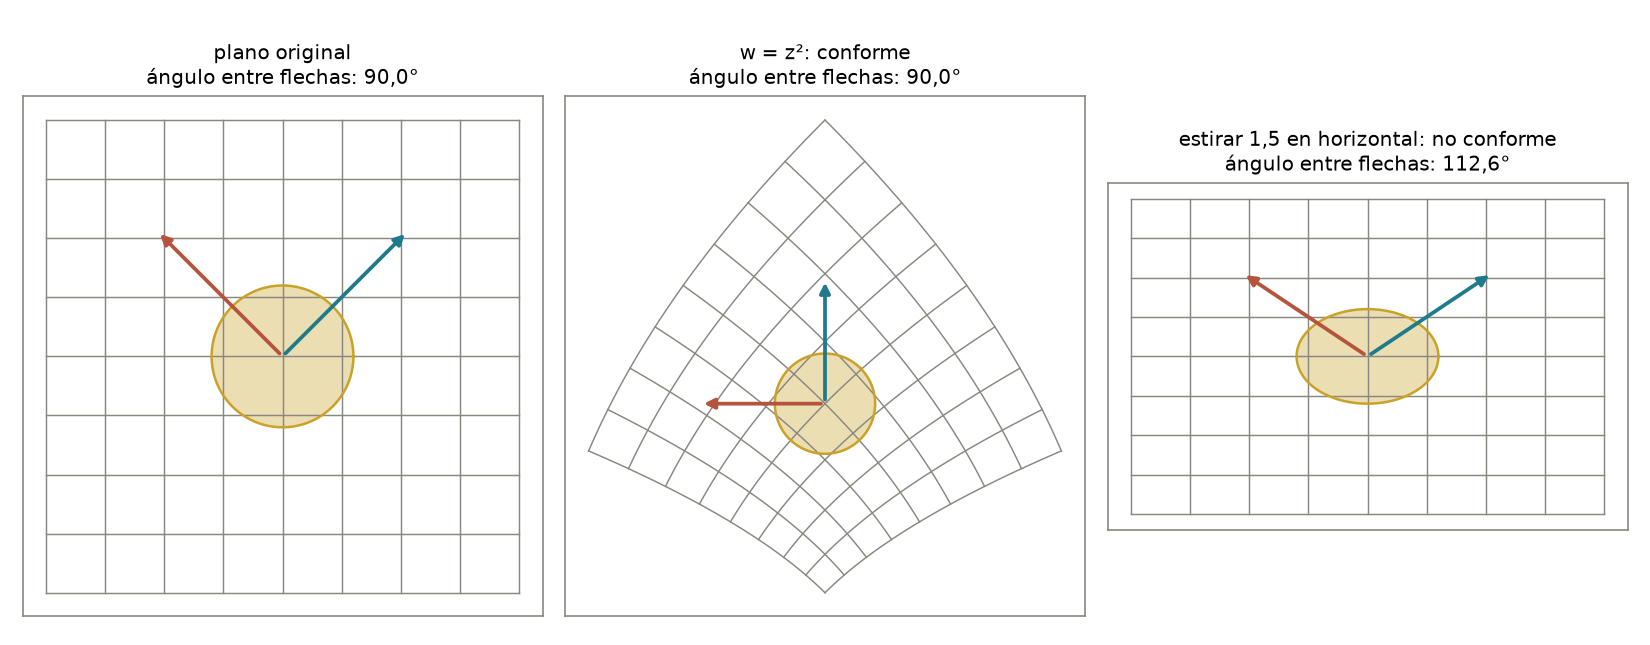
\includegraphics[width=\linewidth]{figuras/conformes/conf_cuadricula.png}
\caption{Una cuadrícula chica alrededor de \(1+i\) (izquierda), su imagen por \(w=z^2\)
(centro) y su imagen por el estiramiento \(\operatorname{diag}(1{,}5;\ 1)\) (derecha). Las
flechas son dos direcciones a \(90^\circ\) y el círculo, uno chico centrado en el punto. En
el centro, flechas y círculo están dibujados con la lupa \(f'(1+i)\): las líneas de la
cuadrícula se curvan pero se siguen cortando a \(90^\circ\), y el círculo sigue siendo círculo.
A la derecha las flechas pasan a formar \(112{,}6^\circ\) y el círculo se vuelve elipse.
Generada con \texttt{apunte/scripts/c2\_conformes.py}.}
\label{fig:conf-cuadricula}
\end{figure}

\paragraph{El conjugado complejo: transponer es reflejar.}\phantomsection\label{sec:conjugado-complejo}
Para un número complejo \(z=a+ib\) se escribe
\(J(z)=\left(\begin{smallmatrix}a&-b\\b&a\end{smallmatrix}\right)\), la matriz de (iv): la de
multiplicar por \(z\), que es la jacobiana de \(\zeta\mapsto z\zeta\). El conjugado
\(\bar z=a-ib\) tiene una lectura matricial directa.

\begin{proposicion}[El conjugado complejo como transpuesta y como reflexión]\label{prop:conjugado-complejo}
Sea \(z=a+ib\) y \(S=\operatorname{diag}(1,-1)\). Entonces
\[
  J(\bar z)=J(z)^T=S\,J(z)\,S
  \qquad\text{y}\qquad
  \lvert z\rvert^2=\det J(z).
\]
\end{proposicion}

\begin{demostracion}
Es una cuenta. Por definición, \(J(\bar z)=J(a+i(-b))=\left(\begin{smallmatrix}a&b\\-b&a\end{smallmatrix}\right)\),
que es \(J(z)^T\). Multiplicar a izquierda por \(S\) cambia el signo de la segunda fila y
multiplicar a derecha por \(S\) cambia el signo de la segunda columna:
\[
  S\,J(z)\,S=\begin{pmatrix}1&0\\0&-1\end{pmatrix}\begin{pmatrix}a&-b\\b&a\end{pmatrix}
  \begin{pmatrix}1&0\\0&-1\end{pmatrix}
  =\begin{pmatrix}a&-b\\-b&-a\end{pmatrix}\begin{pmatrix}1&0\\0&-1\end{pmatrix}
  =\begin{pmatrix}a&b\\-b&a\end{pmatrix}=J(\bar z).
\]
Por último, \(\det J(z)=a\cdot a-(-b)\cdot b=a^2+b^2=z\bar z=\lvert z\rvert^2\). Por ejemplo,
con \(z=3+4i\): \(J(z)^T=\left(\begin{smallmatrix}3&4\\-4&3\end{smallmatrix}\right)=J(3-4i)\)
y \(\det J(z)=9+16=25=\lvert3+4i\rvert^2\).
\end{demostracion}

Tres lecturas. Primera: \emph{transponer la matriz de \(z\) es conjugar \(z\)}; de ahí que
\(J(z)J(z)^T=J(z\bar z)=\lvert z\rvert^2I\), es decir, \(J(z)/\lvert z\rvert\) es ortogonal, la
rotación \(R(\theta)\) de (i). Segunda: la aplicación \(z\mapsto\bar z\), \((a,b)\mapsto(a,-b)\),
tiene matriz \(S\): es la \emph{reflexión en el eje real}. No es multiplicar por ningún
complejo (\(S\) no tiene la forma \(J(w)\) y \(\det S=-1\)); como \(\arg\bar z=-\arg z\),
invierte el sentido de giro. \(S\) es ortogonal, así que cumple (iii) con \(k=1\) y conserva
el tamaño de los ángulos, pero con \(\det S<0\): es \emph{anticonforme}, el caso que la
hipótesis \(\det J>0\) deja afuera en el resultado anterior. Es lo que registra la columna
Reflexión del cuadro~\ref{tab:conserva}: distancias y ángulos, sí; sentido de giro, no.
Tercera: como \(S^{-1}=S\), la igualdad \(J(\bar z)=S^{-1}J(z)\,S\) dice que \(J(\bar z)\) es
\emph{conjugada} de \(J(z)\) por \(S\) en el sentido de la sección~\ref{sec:conjugacion}:
multiplicar por \(\bar z\) es reflejar, multiplicar por \(z\) y volver a reflejar,
\(\bar z\,w=\overline{z\,\bar w}\). La palabra \enquote{conjugado} aparece así con dos sentidos que
acá coinciden; el glosario de la sección~\ref{sec:glosario} los separa.

\begin{atencion}[¿Sobre qué Jacobiano pedimos \(J^TJ=k^2I\)? Coordenadas \((\varphi,\lambda)\) vs.\ metros en el plano tangente]
\emph{En coordenadas.} Si derivamos la carta \(\Phi(\varphi,\lambda)=(x,y)\) respecto de las
coordenadas geodésicas en radianes, obtenemos el Jacobiano de coordenadas
\(J_{\varphi,\lambda}=\partial(x,y)/\partial(\varphi,\lambda)\). Pero \((\varphi,\lambda)\) no
están en metros ni son isótropas: el elipsoide tiene la primera forma fundamental
\(\mathbf G=\operatorname{diag}(M^2,\,N^2\cos^2\varphi)\) (la matriz de la primera forma, con
\(E=M^2\), \(F=0\), \(G=N^2\cos^2\varphi\)). La condición exacta de conformidad es
entonces
\[
  J_{\varphi,\lambda}^T\,J_{\varphi,\lambda}=k(\varphi,\lambda)^2\,\mathbf G
  =k^2\begin{pmatrix}M^2&0\\0&N^2\cos^2\varphi\end{pmatrix}.
\]
Pedir \(J_{\varphi,\lambda}^TJ_{\varphi,\lambda}=k^2I\) directo sobre \((\varphi,\lambda)\)
sería el error de la hoja cuadriculada de la sección~0: tratar radianes de latitud y de
longitud como si midieran lo mismo.

\emph{En metros.} Cuando pasamos a la base ortonormal en metros del plano tangente
(\(ds_{\text{mer}}=M\,d\varphi\), \(ds_{\text{par}}=N\cos\varphi\,d\lambda\)), el Jacobiano
físico es
\[
  \tilde J=J_{\varphi,\lambda}\,\mathbf G^{-1/2}
  =J_{\varphi,\lambda}\,\operatorname{diag}\!\Bigl(\frac1M,\,\frac1{N\cos\varphi}\Bigr),
\]
y recién ahí la condición toma la forma euclídea \(\tilde J^T\tilde J=k^2I\) (con
\(\det\tilde J>0\) para conservar la orientación). El \(\tilde J\) es el que mira la unidad
(la cara~(i) de arriba), y \(h\) y \(k\) son sus escalas en meridiano y paralelo.
\end{atencion}

\paragraph{Conforme es una propiedad local.} Una proyección conforme conserva exactamente
el ángulo en el punto donde se cortan dos curvas y lleva circulitos infinitesimales en
circulitos. Pero el factor de escala \(k(P)\) varía con la posición, así que las figuras
extensas no mantienen ni su área ni su forma global (Groenlandia en Mercator parece del
tamaño de África). Por eso, en la Argentina, POSGAR divide el país en 7 fajas de
Gauss--Krüger de \(3^\circ\) de ancho: no para \enquote{mantener la conformidad} (Gauss--Krüger
ya es conforme a cualquier distancia del meridiano central), sino para acotar la
deformación lineal \(k-1\approx\tfrac12\,\Delta\lambda^2\cos^2\varphi\) (con \(\Delta\lambda\)
en radianes) por debajo de unos \(2{,}3\times10^{-4}\), es decir \(23\) cm/km, en el borde de la
faja (\(\Delta\lambda=1{,}5^\circ\), es decir longitud \(-58{,}5^\circ\)) a la latitud de Buenos Aires
(\(\varphi=-34{,}6^\circ\)). La cifra se calcula sobre el elipsoide GRS80 (\(a=6\,378\,137\) m,
\(1/f=298{,}257222101\); POSGAR 2007, faja 5 de meridiano central \(-60^\circ\), \(k_0=1\)): la aproximación da \(2{,}32\times10^{-4}\) y el
factor de escala exacto, \(2{,}33\times10^{-4}\). Los \(34\) cm/km corresponden al
ecuador (\(\cos\varphi=1\), \(3{,}45\times10^{-4}\) exacto), que es el peor caso de la
faja.

\paragraph{Por qué (iii) es \enquote{conservar ángulos}.} El ángulo entre dos pasitos \(p,q\)
del terreno se calcula con el producto interno, \(\cos\alpha=p\cdot q/(\|p\|\|q\|)\). En el
mapa los pasitos son \(Jp\) y \(Jq\), y \((Jp)\cdot(Jq)=p^T(J^TJ)q=k^2\,p\cdot q\): el
numerador se multiplica por \(k^2\), cada norma por \(k\), y el coseno no cambia. Es el
mismo argumento del capítulo de rotaciones (el producto interno es invariante por rotaciones) con una
homotecia más. Y es lo único que lo logra: si \(J^TJ\) no fuera múltiplo de la identidad,
sus dos autovectores (las direcciones \(v_1,v_2\) de la SVD) se estirarían distinto y
alguna dirección intermedia giraría respecto de las otras.

\paragraph{Cuánto se deforma un ángulo cuando no es conforme.} Con la SVD podemos
medirlo. En las bases \(v_1,v_2\) y \(u_1,u_2\) la jacobiana es \(\operatorname{diag}(\sigma_1,\sigma_2)\),
\(\sigma_1\ge\sigma_2>0\). La dirección de ángulo \(\alpha\) del terreno,
\((\cos\alpha,\sin\alpha)\), va a \((\sigma_1\cos\alpha,\sigma_2\sin\alpha)\), de ángulo
\(\alpha'\) con \(\tan\alpha'=r\tan\alpha\), \(r=\sigma_2/\sigma_1\le1\). El giro de esa
dirección es \(\delta=\alpha-\alpha'\), con
\[
  \tan\delta=\frac{\tan\alpha-\tan\alpha'}{1+\tan\alpha\tan\alpha'}
  =\frac{(1-r)\,t}{1+r\,t^2},\qquad t=\tan\alpha .
\]
Derivando en \(t\) y anulando, \(1+rt^2-2rt^2=0\), o sea \(t^2=1/r\): el giro es máximo
en la dirección con \(\tan\alpha=\sqrt{\sigma_1/\sigma_2}\), y ahí
\(\tan\alpha'=\sqrt{\sigma_2/\sigma_1}=1/\tan\alpha\), de modo que \(\alpha+\alpha'=90^\circ\):
la dirección y su imagen son simétricas respecto de la diagonal de la elipse. En ese
máximo \(\tan\delta=(1-r)/(2\sqrt r)\), y pasando a seno
(\(\sin\delta=\tan\delta/\sqrt{1+\tan^2\delta}\), con \((1-r)^2+4r=(1+r)^2\)):
\[
  \sin\delta_{\max}=\frac{1-r}{1+r}=\frac{\sigma_1-\sigma_2}{\sigma_1+\sigma_2}.
\]
La dirección simétrica, de ángulo \(-\alpha\), gira lo mismo en sentido contrario, así
que el ángulo \(2\alpha\) entre ambas es el que más cambia, y cambia en
\[
  \boxed{\ \omega=2\arcsin\frac{\sigma_1-\sigma_2}{\sigma_1+\sigma_2}\ }
\]
(deformación angular máxima de Tissot). Control: \(\omega=0\) si y solo si
\(\sigma_1=\sigma_2\), que es (ii). Con \(r=1/2\), \(\omega=38{,}94^\circ\), lo mismo
que da maximizar numéricamente \(2(\alpha-\alpha')\).

\begin{ejemplo}[Una foto estirada parejo no es conforme]\label{ej:conf-foto}
Estirar una foto un 50 por ciento en horizontal es aplicarle \(J=\operatorname{diag}(1{,}5;\ 1)\),
la misma matriz en todos los puntos. Las direcciones horizontal y vertical son las de la SVD
y siguen perpendiculares. La diagonal de \(45^\circ\), \((1,1)\), va a \((1{,}5;\ 1)\), de
ángulo \(\arctan(1/1{,}5)=33{,}69^\circ\), y la de \(135^\circ\) va a la simétrica: el ángulo
recto entre las dos diagonales se dibuja de \(112{,}62^\circ\). Con \(r=1/1{,}5\), la fórmula de
Tissot da \(\omega=2\arcsin\frac{0{,}5}{2{,}5}=23{,}07^\circ\), algo más que los
\(22{,}62^\circ\) de las diagonales: el máximo ocurre en la dirección
\(\alpha=\arctan\sqrt{1{,}5}=50{,}77^\circ\), que va a \(39{,}23^\circ\) (suman \(90^\circ\), como
predice la cuenta de arriba). Ningún estiramiento en una sola dirección es conforme, por más
parejo que sea; una conforme puede cambiar el tamaño de un lugar a otro, pero en cada lugar
estira igual en todas las direcciones (figura~\ref{fig:conf-cuadricula}, derecha).
\end{ejemplo}

\unidadInteractiva{15_transformaciones_conformes}{Transformaciones conformes}{Explorá: en «caso precargado» elegí el mapa complejo en el plano. Con la función compleja \(w=z^2\), comprobá que el círculo sigue siendo círculo y que el ángulo entre las dos visuales no cambia al mover «rumbo α (°) de la primera visual». Después pasá a la función \(w=z+\alpha\bar z\), mové el deslizador de \(\alpha\) desde \(0\) y mirá cómo el círculo se vuelve elipse, como la foto estirada del ejemplo~\ref{ej:conf-foto}.}

\subsection{Aplicación topográfica: el factor de escala de Gauss-Krüger en la faja 5}\label{sec:conformes-aplicacion}

Contada en llano, la situación es esta. Quien mide un terreno no anota latitudes y longitudes
sino coordenadas planas en metros, \((E,N)\): cuántos metros al este y cuántos al norte de un
origen. Para pasar de la superficie curva al plano, la Argentina usa una proyección conforme
(la de Gauss-Krüger, la transversa de Mercator de la sección~\ref{sec:conformes-elipsoide})
aplicada por franjas angostas: cada \emph{faja} es una franja de \(3^\circ\) de longitud de
ancho con su propio meridiano central, y el marco oficial de coordenadas del país, POSGAR 2007,
numera esas franjas del 1 al 7. Por ser conforme, un ángulo recto medido en el terreno se
dibuja recto en el plano en cualquier lugar de la franja. Lo que se paga es la escala: sobre
el meridiano central un kilómetro del terreno es un kilómetro del plano, y a medida que nos
alejamos hacia el este o el oeste el plano estira un poco. ¿Cuánto? Lo calculamos en la
franja 5, la de meridiano central \(\lambda_0=-60^\circ\), que es la de la ciudad de Buenos
Aires.

\paragraph{Qué pedimos y a quién.} Usamos la biblioteca \texttt{pyproj} (versión \texttt{3.8.0}, sobre
PROJ \texttt{9.8.1}), que implementa las proyecciones oficiales. Le pedimos el sistema de coordenadas
de código EPSG:5347 (\enquote{POSGAR 2007 / Argentina 5}), que trae meridiano central
\(-60^\circ\), factor de escala \(1\) sobre él y \(5\,500\,000\) m sumados al este para que no
haya coordenadas negativas (por eso importa la diferencia \(\Delta E\), el este menos esos
\(5\,500\,000\) m, y no el número completo). Tomamos cuatro puntos sintéticos, todos a la latitud
de ejemplo \(\varphi=-34{,}6^\circ\), a \(\Delta E=0\), \(50\), \(100\) y \(150\) km al este del
meridiano central. Para cada uno, el script busca la longitud que da ese \(\Delta E\) y le pide
a la función \texttt{get\_factors} de \texttt{pyproj.Proj} la escala a lo largo del meridiano,
la escala a lo largo del paralelo y la convergencia de meridianos (el ángulo entre el norte
del plano y el meridiano del lugar). PROJ declara para ese código el elipsoide WGS84, que para
estas cifras es el mismo que GRS80 (capítulo~\ref{cap:elipsoide}).

\paragraph{La cuenta de bolsillo.} Junto al valor exacto ponemos la aproximación
\[
  k\approx1+\frac{(\Delta E)^2}{2R^2},
\]
con \(R\) el radio medio \(R_1=(2a+b)/3=6\,371\,008{,}771\) m del capítulo del elipsoide
(figura~\ref{fig:elip-radios}). De dónde sale lo mostramos en la
sección~\ref{sec:conformes-escala-serie}; en una esfera de radio \(R\) es la escala de la
transversa de Mercator hasta segundo orden.

\begin{ejemplo}[El factor de escala a \(0\), \(50\), \(100\) y \(150\) km del meridiano central]\label{ej:conf-faja5}
Valores de \texttt{pyproj} y de la aproximación con \(R_1\), en \(\varphi=-34{,}6^\circ\); la
columna \enquote{diferencia} es exacto menos aproximado.

{\small
\begin{center}
\begin{tabular}{r r r r r r r}
\toprule
\(\Delta E\) (km) & \(\lambda\) & \(k\) (\texttt{pyproj}) & \(k-1\) (cm/km) & aprox.\ (cm/km) & diferencia (mm/km) & convergencia\\
\midrule
0 & \(-60^\circ\) & 1{,}00000000 & 0{,}00 & 0{,}00 & 0{,}000 & \(0^\circ\)\\
50 & \(-59{,}4549^\circ\) & 1{,}00003080 & 3{,}08 & 3{,}08 & 0{,}005 & \(-0{,}3095^\circ\)\\
100 & \(-58{,}9099^\circ\) & 1{,}00012321 & 12{,}32 & 12{,}32 & 0{,}022 & \(-0{,}6191^\circ\)\\
150 & \(-58{,}3648^\circ\) & 1{,}00027722 & 27{,}72 & 27{,}72 & 0{,}056 & \(-0{,}9287^\circ\)\\
\bottomrule
\end{tabular}
\end{center}
}

En los cuatro puntos la escala a lo largo del meridiano y la escala a lo largo del paralelo
que devuelve \texttt{pyproj} coinciden (difieren en menos de \(10^{-9}\), el error de la
derivada numérica): es la cara (ii) de las transformaciones conformes, \(\sigma_1=\sigma_2\),
leída en una biblioteca oficial.
\end{ejemplo}

\paragraph{Lectura.} Primero, el estiramiento crece con el cuadrado de la distancia: al
duplicar \(\Delta E\) de \(50\) a \(100\) km, \(k-1\) se multiplica por cuatro, de \(3{,}08\) a
\(12{,}32\) cm por kilómetro (figura~\ref{fig:conf-k}). Segundo, el último punto está fuera de
la franja: en esta latitud el borde, \(\lambda=-58{,}5^\circ\), queda a \(137{,}6\) km del
meridiano central, y ahí \(k-1\) llega a \(2{,}33\times10^{-4}\), los \(23\) cm/km del párrafo
\enquote{Conforme es una propiedad local}. Partir el país en franjas angostas es lo que mantiene
el estiramiento por debajo de eso. Tercero, la cuenta de bolsillo alcanza de sobra: con
\(R_1\) se equivoca en \(0{,}056\) mm por kilómetro a \(150\) km, y con el radio
\(\sqrt{MN}=6\,370\,503{,}553\) m de esa latitud, en \(0{,}012\) mm por kilómetro
(figura~\ref{fig:conf-exacta-aprox}). Cuarto, como las áreas se multiplican por \(k^2\), a
\(150\) km del meridiano central una hectárea del terreno ocupa en el plano
\(10\,000+5{,}55\) m\(^2\). Por último, la convergencia de meridianos crece casi en proporción a la diferencia de
longitud (ejercicio~\ref{ex:conf-convergencia}).

\begin{figure}[htbp]
\centering
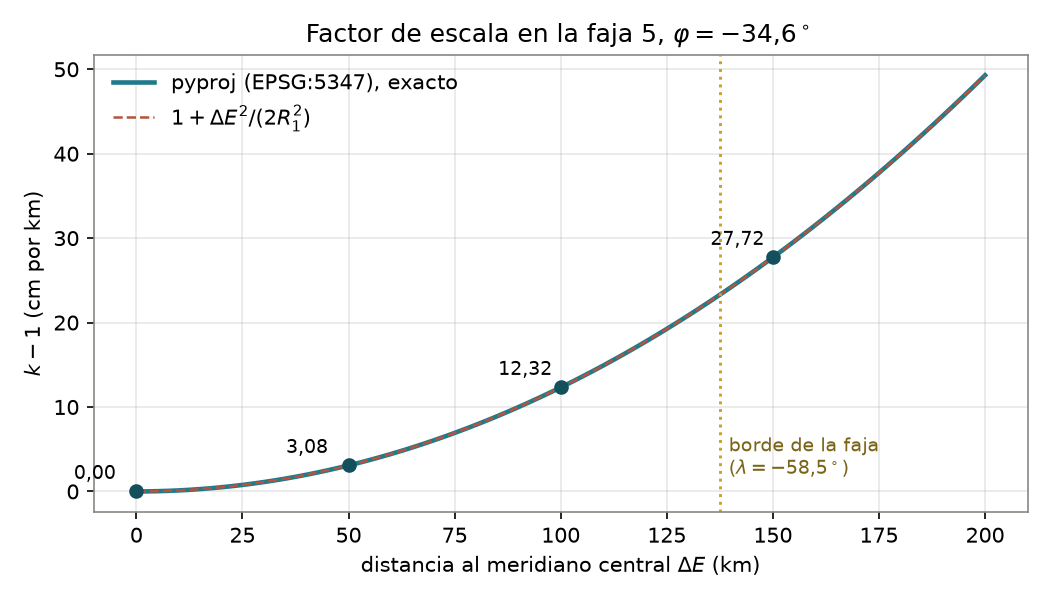
\includegraphics[width=.8\linewidth]{figuras/conformes/conf_k_DeltaE.png}
\caption{Estiramiento \(k-1\), en centímetros por kilómetro, en función de la distancia
\(\Delta E\) al meridiano central de la franja 5, a la latitud de ejemplo
\(\varphi=-34{,}6^\circ\). Línea llena: \texttt{pyproj} \texttt{3.8.0} con EPSG:5347; trazos: la
aproximación \(1+\Delta E^2/(2R_1^2)\), que a esta escala no se distingue. Los puntos son los del
ejemplo~\ref{ej:conf-faja5} y la línea punteada, el borde de la franja.}
\label{fig:conf-k}
\end{figure}

\begin{figure}[htbp]
\centering
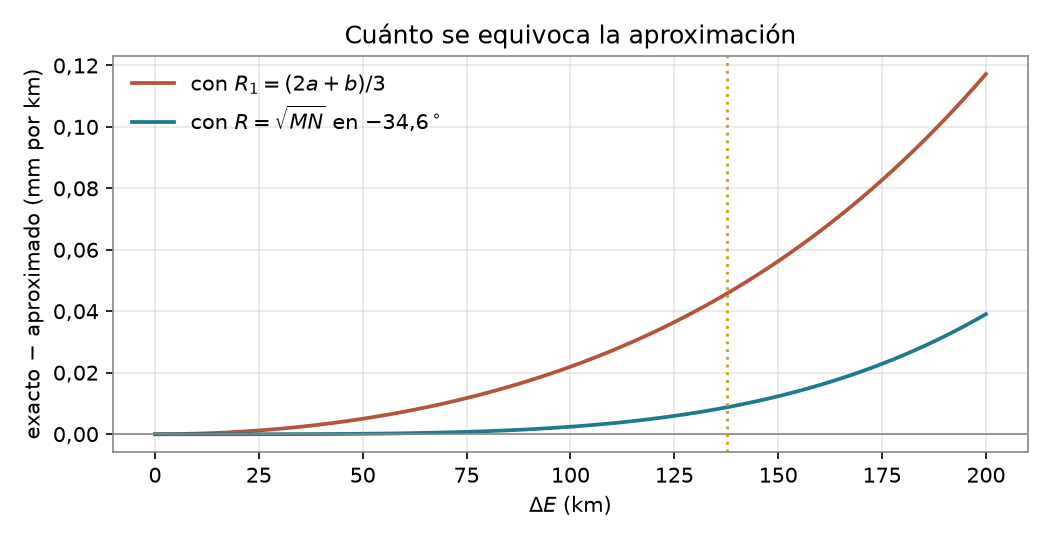
\includegraphics[width=.8\linewidth]{figuras/conformes/conf_exacta_aprox.png}
\caption{Diferencia entre la escala exacta (\texttt{pyproj}) y la aproximada, en milímetros por
kilómetro, con el radio medio \(R_1\) y con el radio \(\sqrt{MN}\) de la latitud de ejemplo.
Dentro de la franja (a la izquierda de la línea punteada) las dos quedan por debajo de
\(0{,}05\) mm por kilómetro; \(\sqrt{MN}\) es mejor por la razón que da la
sección~\ref{sec:conformes-escala-serie}.}
\label{fig:conf-exacta-aprox}
\end{figure}

En la práctica, lo que esto dice es que una distancia medida en el terreno no se copia tal
cual al plano: se multiplica por el \(k\) del lugar. Un lado de un kilómetro a \(100\) km del
meridiano central se dibuja \(12{,}3\) cm más largo; los ángulos, en cambio, pasan sin
corrección de escala. La dependencia de los radios con la latitud se puede explorar en la
unidad del elipsoide.

{\small\linkUnidad{13_elipsoide}{Simulación interactiva: geometría del elipsoide (los radios \(M\), \(N\) y \(\sqrt{MN}\) según la latitud)}\par}

\section{En profundidad}

Con el lenguaje ya armado, estudiamos las proyecciones principales del elipsoide al plano y las leemos según qué propiedad geométrica conservan.

\subsection{Las proyecciones del elipsoide con este lenguaje}\label{sec:conformes-elipsoide}

\paragraph{Cinco maneras de llevar el elipsoide al plano.} Apoyándonos en la métrica y el arco de meridiano del capítulo~\ref{cap:elipsoide}, recorremos cinco construcciones clásicas
integrando una condición cada vez y leyéndolas con las cuatro caras. Sobre el
elipsoide, con la base \((\varphi,\lambda)\),
\[
  ds^2=M^2\,d\varphi^2+N^2\cos^2\varphi\,d\lambda^2 :
\]
\(F=0\), la grilla de meridianos y paralelos es ortogonal, pero un paso \(d\varphi=d\lambda\)
no es un cuadradito: mide \(M\,d\varphi\) hacia el norte y \(N\cos\varphi\,d\lambda\) hacia
el este. En una proyección cilíndrica \(x=a\lambda\), \(y=y(\varphi)\), la jacobiana en las
bases ortonormales del terreno y del plano es diagonal,
\[
  J=\operatorname{diag}(h,k),\qquad
  h=\frac{dy/d\varphi}{M}\ \ (\text{meridiano}),\qquad
  k=\frac{dx/d\lambda}{N\cos\varphi}=\frac{a}{N\cos\varphi}\ \ (\text{paralelo}),
\]
así que \(\{\sigma_1,\sigma_2\}=\{h,k\}\) y cada condición es una ecuación en \(h\) y \(k\).
\begin{enumerate}[label=(\alph*)]
  \item \textbf{Mercator: conforme.} Cara (ii), \(h=k\):
  \[
    \frac{dy}{d\varphi}=\frac{a\,M}{N\cos\varphi}
    \quad\Longrightarrow\quad
    y=a\,q(\varphi),\qquad
    q(\varphi)=\int_0^\varphi\frac{M}{N\cos u}\,du ,
  \]
  la \emph{latitud isométrica}. La integral sale con una identidad: como
  \(M/N=(1-e^2)/(1-e^2\sin^2\varphi)\),
  \[
    \frac{M}{N\cos\varphi}=\frac{1-e^2}{(1-e^2\sin^2\varphi)\cos\varphi}
    =\frac1{\cos\varphi}-\frac{e^2\cos\varphi}{1-e^2\sin^2\varphi}
  \]
  (se verifica poniendo a común denominador: \(1-e^2\sin^2\varphi-e^2\cos^2\varphi=1-e^2\)).
  El primer término integra \(\ln\tan(\pi/4+\varphi/2)\), el de Mercator esférico. En el
  segundo, con \(t=\sin\varphi\), queda \(e^2\int dt/(1-e^2t^2)\), y las fracciones simples
  \(\frac1{1-e^2t^2}=\frac12\bigl(\frac1{1+et}+\frac1{1-et}\bigr)\) dan
  \(\frac e2\ln\frac{1+et}{1-et}\). Por lo tanto
  \[
    \boxed{\ q(\varphi)=\ln\tan\Bigl(\frac\pi4+\frac\varphi2\Bigr)
    -\frac e2\ln\frac{1+e\sin\varphi}{1-e\sin\varphi}\ } .
  \]
  Verificación derivando: \(\frac{d}{d\varphi}\ln\tan(\pi/4+\varphi/2)=1/\cos\varphi\) y
  \(\frac{d}{d\varphi}\frac e2\ln\frac{1+e\sin\varphi}{1-e\sin\varphi}
  =\frac e2\Bigl(\frac{e\cos\varphi}{1+e\sin\varphi}+\frac{e\cos\varphi}{1-e\sin\varphi}\Bigr)
  =\frac{e^2\cos\varphi}{1-e^2\sin^2\varphi}\), que es lo que había que obtener; y
  numéricamente, en \(\varphi=-34{,}6^\circ\), \(q=-0{,}640531\) tanto por la fórmula como
  por \texttt{quad}, y \(a\,q=-4\,085\,391{,}659\) m.
  Lo importante no es la fórmula sino lo que hace: en las coordenadas \((\lambda,q)\), con
  \(d\varphi=(N\cos\varphi/M)\,dq\), la métrica del elipsoide queda
  \[
    ds^2=N^2\cos^2\varphi\,\bigl(dq^2+d\lambda^2\bigr),
  \]
  múltiplo escalar de la métrica plana: cara (iii) con \(k=N\cos\varphi\). La grilla
  \((\lambda,q)\) \emph{es} la carta conforme, y Mercator es simplemente dibujarla con
  \(x=a\lambda\), \(y=aq\).
  \item \textbf{Cilíndrica equivalente.} Conservar áreas es \(\det J=hk=1\):
  \[
    \frac{dy}{d\varphi}=\frac{MN\cos\varphi}{a}\quad\Longrightarrow\quad
    y=\frac1a\int_0^\varphi MN\cos u\,du ,
  \]
  que suele escribirse \(\tfrac a2\,q_A(\varphi)\) (\(q_A\), de \enquote{autálica}, para no
  confundirla con la latitud isométrica \(q\)). Los ángulos no se conservan: \(h=1/k\neq k\) salvo en el
  ecuador.
  \item \textbf{Cilíndrica equidistante.} Meridianos a escala verdadera, \(h=1\):
  \(y=S(\varphi)\), el arco de meridiano del capítulo~\ref{cap:elipsoide}. Ni
  conforme ni equivalente: \(\sigma_1=k\), \(\sigma_2=1\).
  \item \textbf{Esfera autálica.} El área del elipsoide se integra con la misma jacobiana
  \(3\times2\) de la sección~\ref{sec:metrica}: el elemento de área es
  \(\sqrt{EG-F^2}\,d\varphi\,d\lambda=MN\cos\varphi\,d\varphi\,d\lambda\), y
  \[
    A=\int_{-\pi/2}^{\pi/2}2\pi N\cos\varphi\,M\,d\varphi
    =2\pi a^2(1-e^2)\int_{-1}^{1}\frac{dt}{(1-e^2t^2)^2}
  \]
  \[
    \phantom{A}=2\pi a^2(1-e^2)\Bigl[\frac{t}{2(1-e^2t^2)}+\frac1{4e}\ln\frac{1+et}{1-et}\Bigr]_{-1}^{1},
  \]
  con \(t=\sin\varphi\) y \(MN\cos\varphi=a^2(1-e^2)\cos\varphi/(1-e^2\sin^2\varphi)^2\)
  (la primitiva se verifica derivando, igual que en (a)). Evaluando,
  \[
    \boxed{\ A=2\pi a^2+\pi\frac{b^2}{e}\ln\frac{1+e}{1-e}
    =2\pi a^2\Bigl[1+\frac{1-e^2}{e}\operatorname{artanh}e\Bigr]\ },
    \qquad R_A=\sqrt{\frac{A}{4\pi}} .
  \]
  En GRS80, \(A=510\,065\,621{,}7\) km\(^2\) y \(R_A=6\,371\,007{,}181\) m (la integral
  numérica da lo mismo con nueve cifras);
  para comparar, el radio medio \((2a+b)/3=6\,371\,008{,}771\) m y el de igual volumen
  \(\sqrt[3]{a^2b}=6\,371\,000{,}790\) m: los tres \enquote{radios de la Tierra} difieren en
  metros. Pasar a la esfera autálica es equivalente (cara \(\det J=1\)), no conforme.
  \item \textbf{Transversa de Mercator (Gauss--Krüger), el planteo.} Queremos conforme
  \emph{y} el meridiano central \(\lambda_0\) sin deformación (\(h=k=1\) sobre él), porque
  la Argentina se cubre con fajas de \(3^\circ\) de ancho (POSGAR) donde lo que importa es
  deformar poco cerca del meridiano central, no cerca del ecuador. Con las cuatro caras la
  estrategia es clara: la grilla \((q,\lambda)\) ya es conforme por (a), y por (iv) toda
  función analítica de \(z=q+i(\lambda-\lambda_0)\) también lo es. Buscamos entonces
  \[
    w=\mathrm N+i\,\mathrm E=f(z),\qquad f \text{ analítica},\qquad
    f(q)=S(\varphi(q))\ \text{para } \lambda=\lambda_0 ,
  \]
  con \(S\) el arco de meridiano: sobre el meridiano central el norte es la distancia
  medida y el este es cero. Esa condición fija \(f\) sobre el eje real, y una función
  analítica queda determinada por sus valores en una recta (es la unicidad de la
  prolongación analítica): la carta es única. Para escribirla, desarrollamos en serie de
  Taylor en \(\Delta\lambda=\lambda-\lambda_0\) alrededor del eje real, con
  \('=d/dq\):
  \[
    f(q+i\Delta\lambda)=S+i\,\Delta\lambda\,S'-\frac{\Delta\lambda^2}2S''
    -i\frac{\Delta\lambda^3}6S'''+\cdots
  \]
  Las derivadas respecto de \(q\) son derivadas respecto de \(\varphi\) por
  \(d\varphi/dq=N\cos\varphi/M\): \(S'=M\cdot N\cos\varphi/M=N\cos\varphi\), y
  \(S''=\frac{N\cos\varphi}{M}\frac{d(N\cos\varphi)}{d\varphi}=-N\cos\varphi\sin\varphi\),
  porque \(\frac{d}{d\varphi}(N\cos\varphi)=-M\sin\varphi\) (sale derivando
  \(a\cos\varphi(1-e^2\sin^2\varphi)^{-1/2}\); lo controlamos numéricamente en
  \(-34{,}6^\circ\): \(3\,609\,219{,}47\) por los dos lados). Separando parte real e
  imaginaria, los dos primeros términos de cada coordenada son
  \[
    \mathrm N\approx S(\varphi)+\frac{\Delta\lambda^2}2\,N\sin\varphi\cos\varphi,\qquad
    \mathrm E\approx N\cos\varphi\,\Delta\lambda
    +\frac{\Delta\lambda^3}{6}\,N\cos^3\varphi\,(1-\tan^2\varphi+e'^2\cos^2\varphi),
  \]
  y la escala \(k=|f'(z)|/(N\cos\varphi)\approx1+\tfrac12\Delta\lambda^2\cos^2\varphi\)
  (es \(1\) sobre el meridiano central y crece con el cuadrado de la distancia a él; por
  eso Gauss--Krüger argentino no aplica factor de reducción y las fajas son angostas). El
  término cúbico de \(\mathrm E\) lo transcribimos de la bibliografía, no lo deducimos:
  sale de \(S'''\) con la misma mecánica. Control con los dos primeros términos, en
  \(\varphi=-34{,}6^\circ\) y \(\Delta\lambda=1{,}5^\circ\) (el borde de una faja):
  \(\mathrm N=-3\,831\,240{,}9\) m, \(\mathrm E=137\,595{,}3\) m, contra
  \(-3\,831\,241{,}1\) y \(137\,600{,}9\) de \texttt{pyproj} (\texttt{tmerc}, GRS80):
  \(0{,}2\) m en el norte y \(5{,}6\) m en el este, que es el término cúbico que falta.
  Queda como desarrollo complementario; lo que la materia aporta es el planteo:
  \emph{conforme} es \enquote{analítica}, y \enquote{sin deformación sobre el meridiano central} es la
  condición de contorno que la vuelve única.
\end{enumerate}

\begin{resultado}[Buenos Aires y Ushuaia en las tres cilíndricas, GRS80]
\(\varphi=-34{,}6^\circ\) (Buenos Aires) y \(\varphi=-54^\circ\) (Ushuaia). Latitud
isométrica \(q\), escalas \(h\) (meridiano) y \(k=a/(N\cos\varphi)\) (paralelo),
deformación angular máxima \(\omega=2\arcsin\frac{|h-k|}{h+k}\) y factor de área \(hk\).

{\small
\begin{center}
\begin{tabular}{l l rrrr}
\toprule
\(\varphi\) & Proyección & \(h\) & \(k\) & \(\omega\) & \(hk\)\\
\midrule
\(-34{,}6^\circ\) & Mercator (\(h=k\)) & 1{,}2136 & 1{,}2136 & \(0^\circ\) & 1{,}4727\\
\(q=-0{,}6405\) & Equidistante (\(h=1\)) & 1{,}0000 & 1{,}2136 & \(11{,}0725^\circ\) & 1{,}2136\\
 & Equivalente (\(hk=1\)) & 0{,}8240 & 1{,}2136 & \(22{,}0423^\circ\) & 1{,}0000\\
\midrule
\(-54^\circ\) & Mercator (\(h=k\)) & 1{,}6976 & 1{,}6976 & \(0^\circ\) & 2{,}8817\\
\(q=-1{,}1188\) & Equidistante (\(h=1\)) & 1{,}0000 & 1{,}6976 & \(29{,}9731^\circ\) & 1{,}6976\\
 & Equivalente (\(hk=1\)) & 0{,}5891 & 1{,}6976 & \(57{,}9945^\circ\) & 1{,}0000\\
\bottomrule
\end{tabular}
\end{center}
}

Lectura: en Mercator un ángulo medido en Ushuaia se dibuja exacto, pero cada metro del
terreno son \(1{,}70\) en el mapa y cada hectárea \(2{,}88\); en la equivalente las áreas
son exactas pero hay direcciones que giran \(29^\circ\): un ángulo de \(119^\circ\) entre dos
alineaciones se dibuja de \(61^\circ\) (las dos direcciones más giradas y sus imágenes son
simétricas respecto de la diagonal, así que el ángulo y su imagen son suplementarios). No hay
proyección con las dos columnas en \(1\): es el \emph{theorema egregium} en números.
\end{resultado}

\paragraph{Control numérico.} Los valores de la tabla, \(q\), \(A\) y \(R_A\) los
calculamos con NumPy y SciPy (\texttt{quad}) en GRS80, \(a=6\,378\,137\) m,
\(f=1/298{,}257222101\), \(e^2=0{,}00669438\): \(M=a(1-e^2)/(1-e^2\sin^2\varphi)^{3/2}\),
\(N=a/(1-e^2\sin^2\varphi)^{1/2}\), \(k=a/(N\cos\varphi)\), y \(h=k\), \(1\), \(1/k\)
según la proyección. En \(-54^\circ\): \(M=6\,377\,306{,}911\) m, \(N=6\,392\,156{,}080\) m,
\(y_{\text{Mercator}}=aq=-7\,135\,562{,}567\) m, \(S=-5\,985\,916{,}028\) m,
\(y_{\text{equivalente}}=-5\,140\,508{,}988\) m. La \(q\) de la fórmula cerrada y la de
la integral numérica coinciden en las seis cifras mostradas, y
\(dq/d\varphi=1{,}697349\) por diferencias finitas, igual a \(M/(N\cos\varphi)\).

\subsection{De dónde sale \texorpdfstring{\(k\approx1+\Delta E^2/(2R^2)\)}{k = 1 + ΔE²/(2R²)}}\label{sec:conformes-escala-serie}

¿Por qué el estiramiento crece con el cuadrado de la distancia, y qué radio va en la
fórmula? Seguimos con la serie del punto (e): \(z=q+i\,\Delta\lambda\), \(w=f(z)\) con
\(f(q)=S(\varphi(q))\) sobre el meridiano central, y la escala
\(k=\lvert f'(z)\rvert/(N\cos\varphi)\), porque un pasito \(dz\) mide \(N\cos\varphi\,\lvert dz\rvert\)
sobre el elipsoide y \(\lvert f'(z)\rvert\,\lvert dz\rvert\) en el plano.

\begin{proposicion}[Escala de la transversa de Mercator hasta segundo orden]\label{prop:conf-escala-serie}
A la latitud \(\varphi\) y a una diferencia de longitud \(\Delta\lambda\) (en radianes) del
meridiano central,
\[
  k^2=1+\Delta\lambda^2\cos^2\varphi\,\frac NM+O(\Delta\lambda^4),
  \qquad
  k\approx1+\frac12\,\Delta\lambda^2\cos^2\varphi\,\frac NM ,
\]
y, en términos de la distancia al meridiano central,
\(k\approx1+\dfrac{(\Delta E)^2}{2MN}\). En la esfera de radio \(R\) (\(M=N=R\)),
\(k\approx1+(\Delta E)^2/(2R^2)\).
\end{proposicion}

\begin{demostracion}
Derivando la serie de Taylor del punto (e) respecto de \(z\),
\[
  f'(z)=S'+i\,\Delta\lambda\,S''-\frac{\Delta\lambda^2}{2}\,S'''+O(\Delta\lambda^3),
\]
con \('=d/dq\). La parte real es \(S'-\tfrac12\Delta\lambda^2S'''\) y la imaginaria
\(\Delta\lambda\,S''\), así que
\[
  \lvert f'(z)\rvert^2=S'^2+\Delta\lambda^2\bigl(S''^2-S'S'''\bigr)+O(\Delta\lambda^4).
\]
Ya tenemos \(S'=N\cos\varphi\) y \(S''=-N\cos\varphi\sin\varphi\). Para obtener \(S'''\),
derivamos \(S''\) respecto de \(q\) con la regla
\(d/dq=(N\cos\varphi/M)\,d/d\varphi\) y la derivada
\(d(N\cos\varphi)/d\varphi=-M\sin\varphi\) del punto (e):
\[
  \frac{d}{d\varphi}\bigl(N\cos\varphi\sin\varphi\bigr)=-M\sin^2\varphi+N\cos^2\varphi,
  \qquad
  S'''=-\frac{N\cos\varphi}{M}\bigl(N\cos^2\varphi-M\sin^2\varphi\bigr).
\]
Entonces
\[
  S''^2-S'S'''=N^2\cos^2\varphi\sin^2\varphi
  +\frac{N^2\cos^2\varphi}{M}\bigl(N\cos^2\varphi-M\sin^2\varphi\bigr)
  =N^2\cos^2\varphi\cdot\frac{N\cos^2\varphi}{M},
\]
porque los términos en \(\sin^2\varphi\) se cancelan. Dividiendo por \(S'^2=N^2\cos^2\varphi\)
queda \(k^2=1+\Delta\lambda^2\cos^2\varphi\,N/M+O(\Delta\lambda^4)\), y la raíz,
\(\sqrt{1+x}=1+\tfrac x2+O(x^2)\), da la segunda fórmula. Para pasar a \(\Delta E\) usamos el
primer término del este, \(\Delta E\approx N\cos\varphi\,\Delta\lambda\): \(\Delta\lambda^2\cos^2\varphi\approx(\Delta E)^2/N^2\),
y \(\frac{(\Delta E)^2}{N^2}\cdot\frac NM=\frac{(\Delta E)^2}{MN}\). En la esfera, \(MN=R^2\).
\end{demostracion}

Tres consecuencias. La primera: el radio natural de la cuenta de bolsillo es \(\sqrt{MN}\), el
radio medio de Gauss del lugar (capítulo~\ref{cap:elipsoide}); por eso en la
figura~\ref{fig:conf-exacta-aprox} la curva con \(\sqrt{MN}\) queda más cerca de cero que la de
\(R_1\), que es un promedio de toda la Tierra. La segunda: el factor
\(N/M=1+e'^2\cos^2\varphi\) vale \(1{,}00457\) en \(\varphi=-34{,}6^\circ\), y explica la pequeña
diferencia del párrafo \enquote{Conforme es una propiedad local}: en el borde de la franja,
\(\tfrac12\Delta\lambda^2\cos^2\varphi\) da \(2{,}322\times10^{-4}\), multiplicado por \(N/M\) da
\(2{,}333\times10^{-4}\), y \texttt{pyproj} da \(2{,}333\times10^{-4}\). La tercera: el término
siguiente es de cuarto orden en \(\Delta\lambda\), y a \(150\) km del meridiano central ya no
se nota en milímetros por kilómetro.

\section{Ejercicios con solución}

\begin{ejercicio}\label{ex:conf-exp}
Verificá que \(f(z)=e^z\), con \(z=u+iv\), cumple las ecuaciones de Cauchy--Riemann, y calculá la
escala \(k\) y el giro \(\theta\) de su lupa en \(z=\ln2+i\pi/6\).
\solucion{\(e^z=e^u\cos v+i\,e^u\sin v\), así que \(x=e^u\cos v\) e \(y=e^u\sin v\). Entonces
\(x_u=e^u\cos v=y_v\) y \(x_v=-e^u\sin v=-y_u\): se cumplen en todo el plano, y como
\(f'(z)=e^z\neq0\), \(e^z\) es conforme en todas partes. En \(z=\ln2+i\pi/6\),
\(f'(z)=e^{\ln2}e^{i\pi/6}=2e^{i\pi/6}\): \(k=2\) y \(\theta=30^\circ\). Numéricamente,
\(x_u=y_v=\sqrt3\approx1{,}732051\) y \(x_v=-y_u=-1\).}
\end{ejercicio}

\begin{ejercicio}\label{ex:conf-foto10}
Una foto se estira un 10 por ciento en horizontal. ¿En cuánto cambia el ángulo recto entre
sus dos diagonales? ¿Cuál es la deformación angular máxima \(\omega\)?
\solucion{\(J=\operatorname{diag}(1{,}1;\ 1)\). Las diagonales \((1,1)\) y \((-1,1)\) van a
\((1{,}1;\ 1)\) y \((-1{,}1;\ 1)\), que forman \(95{,}45^\circ\): el ángulo recto se abre
\(5{,}45^\circ\). La fórmula de Tissot da
\(\omega=2\arcsin\frac{0{,}1}{2{,}1}=5{,}46^\circ\), apenas más, porque el máximo no ocurre en
las diagonales sino en \(\alpha=\arctan\sqrt{1{,}1}\). Un estiramiento chico en una dirección
ya tuerce ángulos de varios grados.}
\end{ejercicio}

\begin{ejercicio}\label{ex:conf-lado}
En la franja 5, a la latitud \(\varphi=-34{,}6^\circ\) y a \(100\) km al este del meridiano
central, se mide en el terreno un lado de \(1\,000\) m. ¿Cuánto mide en el plano? Usá el
ejemplo~\ref{ej:conf-faja5}.
\solucion{En el plano mide \(k\cdot1\,000\) m, con \(k=1{,}00012321\): \(1\,000{,}123\) m, unos
\(12{,}3\) cm más. La aproximación con \(R_1\) da lo mismo a esa precisión:
\(100^2/(2\cdot6\,371{,}008771^2)=1{,}232\times10^{-4}\).}
\end{ejercicio}

\begin{ejercicio}\label{ex:conf-10cm}
¿A qué distancia del meridiano central el plano estira \(10\) cm por kilómetro
(\(k-1=10^{-4}\))? Resolvelo con la aproximación y compará con el valor exacto.
\solucion{De \((\Delta E)^2/(2R_1^2)=10^{-4}\) sale \(\Delta E=R_1\sqrt{2\times10^{-4}}=90{,}10\) km.
Resolviendo \(k(\Delta E)=1+10^{-4}\) con \texttt{pyproj} a \(\varphi=-34{,}6^\circ\) da
\(90{,}09\) km. Como \(k-1\) crece con el cuadrado, para la mitad del estiramiento
(\(5\) cm/km) alcanza con dividir la distancia por \(\sqrt2\), no por \(2\).}
\end{ejercicio}

\begin{ejercicio}\label{ex:conf-convergencia}
En una esfera, la convergencia de meridianos de la transversa de Mercator vale, en primera
aproximación, \(\Delta\lambda\sin\varphi\). Comparala con la que da \texttt{pyproj} en el punto a
\(100\) km del ejemplo~\ref{ej:conf-faja5}.
\solucion{El punto está en \(\lambda=-58{,}9099^\circ\), \(\Delta\lambda=1{,}0901^\circ\). Entonces
\(\Delta\lambda\sin(-34{,}6^\circ)=-0{,}6190^\circ=-2\,228{,}5''\), y \texttt{pyproj} da
\(-0{,}6191^\circ=-2\,228{,}7''\): difieren en \(0{,}2''\). El signo depende de la convención del
programa; en valor absoluto, a \(100\) km del meridiano central el norte del plano y el
meridiano del lugar forman algo más de medio grado, y eso sí hay que corregirlo al pasar una
dirección medida al plano.}
\end{ejercicio}

% Complemento C4: Marcos de referencia, grillas y remuestreo
\capituloComplemento[4]{Marcos de referencia, grillas y remuestreo}\label{cap:marcos}

\section{La idea}

\subsection{Sistemas, marcos y grillas}\label{sec:sistemas-marcos}

Un sistema de coordenadas define reglas matemáticas para expresar posiciones. Un marco de
referencia materializa esas reglas en una época concreta mediante puntos, estaciones y
observaciones.

Cuando se cambia de marco pueden bastar traslaciones, rotaciones y escala. Si existen
deformaciones regionales, se utilizan grillas de corrección que asignan desplazamientos
variables según la ubicación. En datos ráster, el cambio de coordenadas obliga además a
remuestrear porque los centros de píxel no coinciden exactamente.

\begin{resultado}[Mapa mental de la materia]
Las primeras transformaciones enseñan a reconocer invariantes. Las afinidades amplían la
familia permitiendo deformaciones. La geometría diferencial lleva esas ideas a superficies
curvas, y la geodesia las aplica al elipsoide, las proyecciones y los marcos de referencia.
\end{resultado}

\begin{idea}[La composición como operación central]
Una operación muy importante es la composición: en general, para
construir un sistema de coordenadas es necesario que haya conmutatividad a la hora de componer
movimientos por coordenadas.
\end{idea}

\section{Construcciones, cuentas y ejemplos}

\subsection{Marcos de referencia y transformaciones geodésicas}

Un sistema de coordenadas indica cómo expresar posiciones; un marco de referencia materializa
ese sistema mediante convenciones, época y puntos o estaciones observadas. Cambiar de marco
puede exigir traslaciones, rotaciones, escala y correcciones espaciales.

\subsubsection{Transformaciones paramétricas}

Las transformaciones tridimensionales de semejanza suelen organizarse como
\[
  X_2=t+(1+\mu)RX_1,
\]
donde \(t\) es una traslación, \(\mu\) una pequeña variación de escala y \(R\) una rotación.
Las fórmulas de Molodensky permiten transformar coordenadas geodésicas considerando cambios
de datum y de elipsoide sin pasar necesariamente por una proyección plana.

\subsubsection{Transformaciones mediante grillas}

Una grilla NTv2 almacena correcciones \(\Delta\varphi,\Delta\lambda\) en nodos regulares. Para
un punto interior se interpolan las correcciones de los cuatro nodos vecinos, típicamente por
interpolación bilineal:
\[
\Delta(u,v)=
(1-u)(1-v)\Delta_{00}
+u(1-v)\Delta_{10}
+(1-u)v\Delta_{01}
+uv\Delta_{11}.
\]
Este enfoque representa deformaciones regionales que una transformación global de pocos
parámetros no puede modelar.

\subsection{Discretización, grillas y remuestreo}

Al pasar de coordenadas continuas a una grilla aparecen decisiones sobre resolución,
origen, orientación y regla de muestreo. Una transformación geométrica rara vez lleva los
centros de píxel exactamente a centros de otra grilla; por eso se requiere remuestreo.

\begin{center}
\begin{tabularx}{.9\textwidth}{>{\bfseries}l X}
\toprule
Método & Característica\\
\midrule
Vecino más próximo & conserva valores originales; apropiado para variables categóricas\\
Bilineal & interpola cuatro celdas; suaviza datos continuos\\
Bicúbico & usa un vecindario mayor; mayor suavidad y costo\\
\bottomrule
\end{tabularx}
\end{center}

El jacobiano de la transformación permite estudiar deformaciones locales y convertir áreas
y densidades entre sistemas de coordenadas.

\section{En profundidad}

\subsection{Conexión con la práctica de Agrimensura}

\begin{center}
\begin{tabularx}{\textwidth}{>{\bfseries}p{47mm} X}
\toprule
Concepto & Aplicación\\
\midrule
Coordenadas geodésicas \((\varphi,\lambda,h)\) & salida y procesamiento de observaciones GNSS\\
Base tangente y métrica & distancias y ángulos locales sobre el elipsoide\\
Radios \(M,N\) & variación geométrica con la latitud\\
Proyección conforme & coordenadas planas para cartografía y mensura\\
Transformaciones de marco & compatibilidad entre realizaciones geodésicas\\
Grillas de corrección & transformación regional de alta precisión\\
Remuestreo & ortomosaicos, modelos de elevación y datos ráster\\
Jacobiano & escala, deformación y propagación local\\
\bottomrule
\end{tabularx}
\end{center}

\begin{idea}[Estrategia de estudio acumulativa]
Cada nuevo tema debería incorporarse con la secuencia
\[
\text{definición}\rightarrow
\text{representación geométrica}\rightarrow
\text{fórmula}\rightarrow
\text{ejemplo numérico}\rightarrow
\text{implementación}.
\]
Para la implementación pueden usarse Python, NumPy, SciPy, SymPy, \texttt{pyproj},
GeographicLib y QGIS según el capítulo.
\end{idea}


\clearpage
\appendix
\chapter{Apéndices}\label{cap:apendices}
% Apéndice: construcción geométrica de las matrices de rotación 3D
\section{Construcción geométrica de las matrices de rotación 3D}\label{cap:14}\label{ap:rot3d}

\subsection{Convención utilizada}

Se consideran vectores columna, rotaciones activas y un sistema cartesiano de mano derecha.
Una rotación activa mueve el vector mientras los ejes permanecen fijos. El sentido positivo
se determina mediante la regla de la mano derecha: el pulgar apunta en la dirección positiva
del eje y los dedos indican el sentido del giro.

\begin{idea}[Principio de construcción]
Una rotación alrededor de un eje:
\begin{itemize}
  \item deja fija la coordenada paralela al eje;
  \item aplica una rotación plana ordinaria en el plano perpendicular;
  \item tiene como columnas las imágenes de \(e_x,e_y,e_z\).
\end{itemize}
No es necesario memorizar tres matrices independientes: todas se reconstruyen a partir de
esta regla.
\end{idea}

\subsection{Recordatorio: rotación en un plano}

En un plano con coordenadas \((u,v)\), una rotación positiva de ángulo \(\theta\) cumple
\[
\begin{pmatrix}u'\\v'\end{pmatrix}
=
\begin{pmatrix}
\cos\theta&-\sin\theta\\
\sin\theta& \cos\theta
\end{pmatrix}
\begin{pmatrix}u\\v\end{pmatrix}.
\]
Por lo tanto,
\[
u'=u\cos\theta-v\sin\theta,
\qquad
v'=u\sin\theta+v\cos\theta.
\]
Para construir una rotación espacial basta identificar cuál es el par de coordenadas que
forma el plano perpendicular al eje.

\subsection{Rotación alrededor del eje \(z\)}

El eje \(z\) permanece fijo y la rotación ocurre en el plano \(xy\). Por lo tanto,
\[
\begin{aligned}
x'&=x\cos\theta-y\sin\theta,\\
y'&=x\sin\theta+y\cos\theta,\\
z'&=z.
\end{aligned}
\]
Agrupando los coeficientes de \(x,y,z\):
\[
\boxed{
R_z(\theta)=
\begin{pmatrix}
\cos\theta&-\sin\theta&0\\
\sin\theta& \cos\theta&0\\
0&0&1
\end{pmatrix}
}.
\]

La misma matriz se obtiene mirando las imágenes de la base:
\[
R_z e_x=
\begin{pmatrix}\cos\theta\\\sin\theta\\0\end{pmatrix},
\qquad
R_z e_y=
\begin{pmatrix}-\sin\theta\\\cos\theta\\0\end{pmatrix},
\qquad
R_z e_z=
\begin{pmatrix}0\\0\\1\end{pmatrix}.
\]
Estos tres vectores son, respectivamente, las tres columnas de \(R_z\).

\begin{center}
\begin{tikzpicture}[scale=1.0]
  \draw[axisline,-{Latex[length=2.4mm]}] (-.3,0)--(5.3,0) node[right] {$x$};
  \draw[axisline,-{Latex[length=2.4mm]}] (0,-.3)--(0,4.5) node[above] {$y$};
  \draw[mainline,-{Latex[length=2.7mm]}] (0,0)--(4,0)
    node[below right] {$e_x$};
  \draw[rust,line width=1.05pt,-{Latex[length=2.7mm]}] (0,0)--(3,2.6)
    node[above right] {$R_ze_x$};
  \draw[teal,line width=.8pt,-{Latex[length=2mm]}] (1.4,0)
    arc[start angle=0,end angle=41,radius=1.4];
  \node[text=teal] at (1.7,.55) {$\theta$};
  \node[font=\small,text=muted,align=center] at (7,2.0)
    {\(z\) sale perpendicular al dibujo\\y permanece fijo};
\end{tikzpicture}
\end{center}

\subsection{Rotación alrededor del eje \(x\)}

Ahora \(x\) permanece constante y la rotación ocurre en el plano \(yz\). Se aplica la misma
matriz plana al par \((y,z)\):
\[
\begin{aligned}
x'&=x,\\
y'&=y\cos\theta-z\sin\theta,\\
z'&=y\sin\theta+z\cos\theta.
\end{aligned}
\]
Por lo tanto,
\[
\boxed{
R_x(\theta)=
\begin{pmatrix}
1&0&0\\
0&\cos\theta&-\sin\theta\\
0&\sin\theta& \cos\theta
\end{pmatrix}
}.
\]
Sus columnas vuelven a ser las imágenes de la base:
\[
R_xe_x=e_x,\qquad
R_xe_y=
\begin{pmatrix}0\\\cos\theta\\\sin\theta\end{pmatrix},
\qquad
R_xe_z=
\begin{pmatrix}0\\-\sin\theta\\\cos\theta\end{pmatrix}.
\]
La primera columna \((1,0,0)^T\) expresa geométricamente que el eje \(x\) permanece fijo.

\subsection{Rotación alrededor del eje \(y\)}

En este caso \(y\) permanece constante y el giro ocurre en el plano \(xz\). La regla de la
mano derecha determina los signos:
\[
\begin{aligned}
x'&=x\cos\theta+z\sin\theta,\\
y'&=y,\\
z'&=-x\sin\theta+z\cos\theta.
\end{aligned}
\]
Así:
\[
\boxed{
R_y(\theta)=
\begin{pmatrix}
\cos\theta&0&\sin\theta\\
0&1&0\\
-\sin\theta&0&\cos\theta
\end{pmatrix}
}.
\]
Por columnas:
\[
R_ye_x=
\begin{pmatrix}\cos\theta\\0\\-\sin\theta\end{pmatrix},
\qquad
R_ye_y=e_y,
\qquad
R_ye_z=
\begin{pmatrix}\sin\theta\\0\\\cos\theta\end{pmatrix}.
\]

\begin{atencion}[Por qué \(R_y\) parece tener signos diferentes]
Si se escribe directamente la rotación 2D sobre el par ordenado \((x,z)\), puede aparecer
una confusión de orientación. Mirado desde el extremo positivo del eje \(y\), el plano
\(xz\) debe orientarse de acuerdo con la regla de la mano derecha. Una comprobación segura es
usar un ángulo de \(90^\circ\): la matriz anterior lleva \(e_x\) a \(-e_z\) y \(e_z\) a
\(e_x\).
\end{atencion}

\subsection{Resumen geométrico}

\begin{center}
\begin{tabularx}{.9\textwidth}{>{\bfseries}c c c}
\toprule
Rotación & Coordenada fija & Plano que rota\\
\midrule
\(R_x\) & \(x\) & \(yz\)\\
\(R_y\) & \(y\) & \(zx\), orientado por mano derecha\\
\(R_z\) & \(z\) & \(xy\)\\
\bottomrule
\end{tabularx}
\end{center}

Cada matriz debe satisfacer cuatro comprobaciones inmediatas:
\[
R_i(0)=I,\qquad
R_i(\theta)^TR_i(\theta)=I,\qquad
\det R_i(\theta)=1,\qquad
R_i(\theta)e_i=e_i.
\]
La última igualdad expresa que el vector director del eje es un autovector con autovalor
\(1\).

\subsection{Rotación alrededor de un eje arbitrario}

Sea \(u\) un vector unitario que define el eje. Todo vector \(v\) puede separarse en una parte
paralela y otra perpendicular:
\[
v=v_\parallel+v_\perp,
\qquad
v_\parallel=(u\cdot v)u,
\qquad
v_\perp=v-(u\cdot v)u.
\]
La rotación deja fija \(v_\parallel\). En el plano perpendicular, \(v_\perp\) gira como en
dos dimensiones y \(u\times v\) proporciona la dirección perpendicular dentro de ese plano:
\[
R(u,\theta)v
=
v_\parallel
+\cos\theta\,v_\perp
+\sin\theta\,(u\times v).
\]
Reagrupando:
\[
\boxed{
R(u,\theta)
=
\cos\theta\,I
+(1-\cos\theta)uu^T
+\sin\theta\,[u]_\times
},
\]
donde
\[
[u]_\times=
\begin{pmatrix}
0&-u_z&u_y\\
u_z&0&-u_x\\
-u_y&u_x&0
\end{pmatrix}.
\]
Esta es la fórmula de Rodrigues. Las matrices \(R_x,R_y,R_z\) se recuperan tomando
\(u=e_x,e_y,e_z\), respectivamente.

\begin{resultado}[Idea central]
Una matriz de rotación 3D se construye dejando fija la componente paralela al eje y rotando
la componente perpendicular como en un plano. Sus columnas muestran dónde terminan los tres
vectores de la base.
\end{resultado}


% Apéndice: rotaciones infinitesimales y orden de composición
\section{Rotaciones infinitesimales y orden de composición}\label{cap:15}\label{ap:infinitesimales}

\subsection{De dónde surge \(R(\varepsilon)\approx I+\varepsilon A\)}

La aproximación surge del desarrollo de Taylor de la matriz de rotación alrededor del ángulo
cero. Para una rotación de ángulo \(\varepsilon\) alrededor del eje \(x\):
\[
R_x(\varepsilon)=
\begin{pmatrix}
1&0&0\\
0&\cos\varepsilon&-\sin\varepsilon\\
0&\sin\varepsilon& \cos\varepsilon
\end{pmatrix}.
\]
Las series de Taylor son
\[
\cos\varepsilon
=1-\frac{\varepsilon^2}{2!}+\frac{\varepsilon^4}{4!}-\cdots,
\qquad
\sin\varepsilon
=\varepsilon-\frac{\varepsilon^3}{3!}+\frac{\varepsilon^5}{5!}-\cdots.
\]
Sustituyendo:
\[
R_x(\varepsilon)=
\begin{pmatrix}
1&0&0\\
0&1-\frac{\varepsilon^2}{2}+\cdots&
-\varepsilon+\frac{\varepsilon^3}{6}-\cdots\\
0&\varepsilon-\frac{\varepsilon^3}{6}+\cdots&
1-\frac{\varepsilon^2}{2}+\cdots
\end{pmatrix}.
\]
Si se conservan únicamente los términos constantes y lineales en \(\varepsilon\):
\[
R_x(\varepsilon)
=
\underbrace{
\begin{pmatrix}
1&0&0\\0&1&0\\0&0&1
\end{pmatrix}}_{I}
+
\varepsilon
\underbrace{
\begin{pmatrix}
0&0&0\\0&0&-1\\0&1&0
\end{pmatrix}}_{A_x}
+O(\varepsilon^2).
\]
Por lo tanto,
\[
\boxed{R_x(\varepsilon)=I+\varepsilon A_x+O(\varepsilon^2)}.
\]
El símbolo \(O(\varepsilon^2)\) reúne todos los términos cuyo tamaño disminuye como
\(\varepsilon^2\) o más rápidamente cuando \(\varepsilon\to0\).

\begin{resultado}[Forma general]
Para una familia suave de rotaciones basada en la identidad, es decir, con \(R(0)=I\), Taylor
alrededor de \(\theta=0\) da
\[
R(\varepsilon)=R(0)+\varepsilon R'(0)+O(\varepsilon^2).
\]
Como \(R(0)=I\), definiendo \(A=R'(0)\) se obtiene
\[
\boxed{R(\varepsilon)=I+\varepsilon A+O(\varepsilon^2)}.
\]
La matriz \(A\) se denomina \textbf{generador infinitesimal} de la rotación.
\end{resultado}

\subsection{Generadores alrededor de los tres ejes}

Con la convención de giros positivos de la mano derecha:
\[
A_x=
\begin{pmatrix}
0&0&0\\
0&0&-1\\
0&1&0
\end{pmatrix},
\quad
A_y=
\begin{pmatrix}
0&0&1\\
0&0&0\\
-1&0&0
\end{pmatrix},
\quad
A_z=
\begin{pmatrix}
0&-1&0\\
1&0&0\\
0&0&0
\end{pmatrix}.
\]
Estas matrices son antisimétricas, \(A_i^T=-A_i\), y describen la velocidad instantánea
con la que se mueve un vector al comenzar la rotación.

\subsection{Interpretación geométrica}

Sea \(e_x=(1,0,0)^T\). Para cualquier vector \(v\),
\[
  A_xv=e_x\times v.
\]
Entonces:
\[
  R_x(\varepsilon)v\approx v+\varepsilon(e_x\times v).
\]
El primer término es el vector original. El segundo es un pequeño desplazamiento perpendicular
al eje \(e_x\) y al vector \(v\), es decir, tangente a la circunferencia recorrida durante
la rotación.

\begin{center}
\begin{tikzpicture}[scale=1.0]
  \coordinate (o) at (1,1);
  \coordinate (v) at (6.2,2.0);
  \coordinate (vp) at (5.85,2.95);
  \draw[axisline,-{Latex[length=2.5mm]}] (o)--(8,1)
    node[right] {eje \(x\)};
  \draw[mainline,-{Latex[length=2.8mm]}] (o)--(v)
    node[midway,below] {$v$};
  \draw[rust,line width=1.05pt,-{Latex[length=2.8mm]}] (v)--(vp)
    node[right] {$\varepsilon A_xv$};
  \draw[teal,dashed] (o)--(vp)
    node[midway,above left] {$R_x(\varepsilon)v$};
  \fill[ink] (o) circle (2.4pt);
  \fill[teal] (v) circle (2.4pt);
  \fill[rust] (vp) circle (2.4pt);
  \node[font=\small,text=muted,align=center] at (5.4,3.8)
    {el desplazamiento infinitesimal\\es tangente a la trayectoria};
\end{tikzpicture}
\end{center}

\begin{idea}[Qué significa geométricamente la aproximación]
Una rotación finita sigue un arco de circunferencia. En un intervalo angular muy pequeño,
el arco y su recta tangente son indistinguibles a primer orden. La expresión
\(v+\varepsilon A_xv\) reemplaza localmente el arco por ese desplazamiento tangencial.
\end{idea}

\subsection{Por qué el orden no aparece a primer orden}

Consideremos dos rotaciones pequeñas:
\[
R_x(\varepsilon)=I+\varepsilon A_x+O(\varepsilon^2),
\qquad
R_y(\delta)=I+\delta A_y+O(\delta^2).
\]
Primero \(R_y\) y después \(R_x\):
\[
\begin{aligned}
R_x(\varepsilon)R_y(\delta)
&\approx(I+\varepsilon A_x)(I+\delta A_y)\\
&=I+\varepsilon A_x+\delta A_y+\varepsilon\delta A_xA_y.
\end{aligned}
\]
En el orden inverso:
\[
\begin{aligned}
R_y(\delta)R_x(\varepsilon)
&\approx(I+\delta A_y)(I+\varepsilon A_x)\\
&=I+\varepsilon A_x+\delta A_y+\varepsilon\delta A_yA_x.
\end{aligned}
\]
Los términos de primer orden son exactamente los mismos. La diferencia es
\[
\boxed{
R_x(\varepsilon)R_y(\delta)
-R_y(\delta)R_x(\varepsilon)
\approx\varepsilon\delta[A_x,A_y]
},
\]
donde
\[
  [A_x,A_y]=A_xA_y-A_yA_x
\]
es el conmutador.

\begin{resultado}[Conclusión precisa]
Las rotaciones infinitesimales no conmutan exactamente. Parecen conmutar cuando se trabaja
solo a primer orden porque la diferencia causada por el orden es proporcional al producto
\(\varepsilon\delta\), que es de segundo orden.
\end{resultado}

\subsection{Interpretación geométrica del cambio de orden}

La primera rotación modifica ligeramente la orientación del objeto sobre el cual actúa la
segunda. Esa modificación es del orden de \(\varepsilon\). Como la segunda rotación tiene
tamaño \(\delta\), el efecto adicional producido por aplicar una sobre la orientación creada
por la otra tiene tamaño \(\varepsilon\delta\).

Si \(\varepsilon=\delta=0.01\) radianes:
\[
\varepsilon=10^{-2},
\qquad
\varepsilon\delta=10^{-4}.
\]
El movimiento principal tiene tamaño aproximado \(10^{-2}\), mientras que la diferencia entre
los dos órdenes aparece aproximadamente en \(10^{-4}\). Al conservar solamente la primera
cifra de pequeñez, esa diferencia desaparece.

\subsection{Relación con la exponencial matricial}

Las rotaciones pueden escribirse exactamente como
\[
  R_x(\varepsilon)=e^{\varepsilon A_x},
  \qquad
  R_y(\delta)=e^{\delta A_y}.
\]
La fórmula de Baker--Campbell--Hausdorff comienza como
\[
e^{\varepsilon A_x}e^{\delta A_y}
=
\exp\left(
\varepsilon A_x+\delta A_y
+\frac12\varepsilon\delta[A_x,A_y]+\cdots
\right).
\]
El conmutador aparece explícitamente como la primera corrección que registra el orden.
Para los generadores de rotaciones:
\[
  [A_x,A_y]=A_z,
\]
de modo que la diferencia entre girar infinitesimalmente alrededor de \(x\) y de \(y\) en
órdenes opuestos se manifiesta como una pequeña rotación residual alrededor de \(z\).

\begin{atencion}[Idea que conviene retener]
\[
\boxed{
\text{A primer orden las rotaciones pequeñas se suman;}
\quad
\text{a segundo orden aparece el orden.}
}
\]
No se afirma que las rotaciones tridimensionales conmuten, sino que su no conmutatividad es
demasiado pequeña para aparecer en la aproximación lineal.
\end{atencion}


% Apéndice: composición afín práctica: rotación y escala
\section{Composición afín práctica: rotación y escala}\label{cap:16}\label{ap:composicion-afin}

\subsection{Rotación alrededor de un centro}

Sea \(c=(c_x,c_y)^T\) y sea \(R\) una matriz de rotación. Trasladar \(c\) al origen, rotar
y trasladar de regreso produce
\[
F_1(x)=c+R(x-c)=Rx+(I-R)c.
\]
En coordenadas homogéneas:
\[
\boxed{
H_1=
\left(
\begin{array}{c|c}
R&(I-R)c\\ \hline
0\quad0&1
\end{array}
\right)
}.
\]
La escritura por bloques significa que \(R\) ocupa las primeras dos filas y columnas, mientras
que el vector \((I-R)c\) ocupa la última columna.

Para \(\theta=45^\circ\):
\[
R=
\begin{pmatrix}
r&-r\\
r&r
\end{pmatrix},
\qquad
r=\frac{\sqrt2}{2}.
\]

\begin{atencion}[Error frecuente con \(45^\circ\)]
Es común escribir en algún pasaje \(\sqrt3/2\). Para \(45^\circ\), el valor correcto es
\[
\sin45^\circ=\cos45^\circ=\frac{\sqrt2}{2}.
\]
\(\sqrt3/2\) corresponde al coseno de \(30^\circ\) o al seno de \(60^\circ\).
\end{atencion}

\subsection{Escala uniforme alrededor de otro centro}

Sea \(d=(d_x,d_y)^T\) y sea \(k\) el factor de escala:
\[
F_2(y)=d+k(y-d)=ky+(1-k)d.
\]
Su matriz homogénea es
\[
\boxed{
H_2=
\begin{pmatrix}
k&0&(1-k)d_x\\
0&k&(1-k)d_y\\
0&0&1
\end{pmatrix}
}.
\]
Con \(k=0.5\), cada distancia al centro \(d\) queda reducida a la mitad.

\subsection{Composición y orden}

La rotación se aplica primero y la escala después:
\[
F=F_2\circ F_1.
\]
Por eso, con vectores columna,
\[
\boxed{H=H_2H_1}.
\]
La matriz situada a la derecha actúa primero. Al desarrollar por bloques:
\[
F(x)=kRx+\left[k(I-R)c+(1-k)d\right].
\]
Así,
\[
A=kR,
\qquad
t=k(I-R)c+(1-k)d.
\]

\subsection{Ejemplo numérico completo}

Se eligen
\[
c=(3,1),\qquad d=(-1,2),\qquad
k=0.5,\qquad \theta=45^\circ.
\]
La rotación alrededor de \(c\) queda
\[
H_1=
\begin{pmatrix}
0.70710678&-0.70710678&1.58578644\\
0.70710678& 0.70710678&-1.82842712\\
0&0&1
\end{pmatrix}.
\]
La escala respecto de \(d\) es
\[
H_2=
\begin{pmatrix}
0.5&0&-0.5\\
0&0.5&1\\
0&0&1
\end{pmatrix}.
\]
El producto es
\[
\boxed{
H=H_2H_1=
\begin{pmatrix}
0.35355339&-0.35355339&0.29289322\\
0.35355339& 0.35355339&0.08578644\\
0&0&1
\end{pmatrix}
}.
\]
Por tanto:
\[
A=
\begin{pmatrix}
0.35355339&-0.35355339\\
0.35355339& 0.35355339
\end{pmatrix},
\qquad
t=
\begin{pmatrix}
0.29289322\\
0.08578644
\end{pmatrix}.
\]

\subsection{Punto fijo}

Un punto \(p\) es fijo si
\[
Ap+t=p.
\]
Por lo tanto:
\[
(I-A)p=t,
\qquad
\boxed{p=(I-A)^{-1}t}.
\]
En este ejemplo:
\[
\boxed{
p_\ast=
\begin{pmatrix}
1-\frac{\sqrt2}{2}\\[1mm]
1-\frac{\sqrt2}{2}
\end{pmatrix}
\approx
\begin{pmatrix}
0.29289322\\
0.29289322
\end{pmatrix}
}.
\]
La verificación directa es
\[
Hp_\ast^{\,h}=p_\ast^{\,h},
\qquad
p_\ast^{\,h}=
\begin{pmatrix}p_{\ast x}\\p_{\ast y}\\1\end{pmatrix}.
\]

\subsection{Autovalores y coordenadas homogéneas}

Como \(H\) es triangular por bloques, sus autovalores son los dos autovalores de \(A=0.5R\)
y el autovalor homogéneo \(1\):
\[
\lambda_{1,2}=0.5e^{\pm i\pi/4},
\qquad
\lambda_3=1.
\]
Los dos autovalores complejos describen conjuntamente la contracción y el giro de la parte
lineal. El autovector real asociado a \(\lambda_3=1\) puede escribirse
\[
v_3=
\begin{pmatrix}p_{\ast x}\\p_{\ast y}\\1\end{pmatrix},
\]
y representa el punto fijo.

\begin{atencion}[Cómo interpretar el resultado de una calculadora online]
Los autovectores se devuelven con una normalización arbitraria. Si la calculadora entrega
\[
v=(u,v,w)^T,\qquad w\neq0,
\]
el punto cartesiano correspondiente es \((u/w,v/w)\). Si \(w=0\), el vector representa una
dirección o punto ideal, no un punto fijo finito. Una matriz homogénea afín siempre posee
\(1\) como autovalor, pero solo hay punto fijo finito cuando existe un autovector asociado
con \(w\neq0\).
\end{atencion}

\subsection{Implementación en Excel}

\begin{enumerate}
  \item Ingresar \(H_1\) en un bloque \(3\times3\), por ejemplo
  \texttt{B2:D4}.
  \item Ingresar \(H_2\) en \texttt{F2:H4}.
  \item Seleccionar un bloque \(3\times3\) para el resultado e introducir
  \[
  \texttt{=MMULT(F2:H4,B2:D4)}.
  \]
  En versiones antiguas de Excel se confirma con
  \texttt{Ctrl+Shift+Enter}; en versiones con matrices dinámicas basta \texttt{Enter}.
  \item Para transformar un punto homogéneo almacenado como columna
  \((x,y,1)^T\), usar
  \[
  \texttt{=MMULT(matriz\_compuesta,rango\_del\_punto)}.
  \]
  \item Para obtener el punto fijo sin recurrir a una web, construir \(I-A\) y calcular
  \[
  \texttt{=MMULT(MINVERSE(rango\_I\_menos\_A),rango\_t)}.
  \]
  El nombre de \texttt{MINVERSE} puede variar según el idioma de Excel.
\end{enumerate}

\begin{idea}[Comprobación mínima]
Transformar todos los vértices de la figura, verificar uno manualmente y comprobar que
\[
Hp_\ast^{\,h}=p_\ast^{\,h}.
\]
En el programa gráfico, los comandos relevantes son \texttt{ROTATE} y
\texttt{SCALE}. El estilo o tamaño del punto puede aumentarse para hacer visibles centros y
vértices.
\end{idea}


% Apéndice: bibliografía comentada por el profesor
\section{Bibliografía comentada por el profesor}\label{cap:20}\label{ap:bibliografia}

\textbf{Material docente.} Lista de la pestaña ``Bibliografía'' del campus, en el orden del
campus, con los comentarios textuales del profesor (entre comillas) y las indicaciones que
dejó en los resúmenes de clase. Los PDF están en la carpeta
\file{Proyectos / Agrimensura / Sistemas de Coordenadas / Bibliografia} de Dropbox; entre corchetes,
el nombre del archivo.

\begin{itemize}
  \item \textbf{Axler}, \emph{Linear Algebra Done Right} [\file{Algebra done right.pdf}].
  Resumen de clase 4: ``el libro del que yo primero saqué el tema [formas lineales] y
  concluí que era importante es el de Axler, que está en inglés''.
  \item \textbf{Gerlach}, \emph{Dual of a Vector Space} [\file{DualOfAVectorSpace.pdf}].
  Complemento para formas lineales y dualidad (sección~\ref{sec:formas-lineales}).
  \item \textbf{Butler}, \emph{Facts About Eigenvalues} [\file{butler-eigenvalues.pdf}].
  \item \textbf{Winitzki}, \emph{Linear Algebra via Exterior Products}
  [\file{Algebra via exterior products.pdf}]. Producto cuña y determinante
  (secciones~\ref{sec:exterior} y~\ref{sec:nucleo}).
  \item \textbf{Strang}, \emph{Álgebra lineal y sus aplicaciones} [\file{Strang-algebra-p1.pdf},
  sólo parte 1].
  \item \textbf{Juan de Burgos}, \emph{Álgebra Lineal y Geometría Cartesiana}
  [\file{Algebra-burgos-p1.pdf}, sólo parte 1]. ``Clase 3. A partir de la página 382 del
  libro de Burgos hay una muy buena explicación de geometría afín, aunque está basada toda en
  expresiones algebraicas. Es bastante importante notar que este enfoque es mixto, no se basa
  directamente en transformaciones lineales pero tampoco se basa en puntos y rectas
  abstractas sino que trabaja en coordenadas cartesianas.'' Resumen de clase 3: ``me parece
  que el que mejor les va a venir es el de Burgos, aunque el escaneo es francamente malo''.
  Resumen de clase 4: ``en castellano el libro que trata lo de formas lineales es el de
  Burgos (el capítulo que dice `espacio dual')''.
  \item \textbf{Azócar}, \emph{El cuerpo de los complejos}
  [\file{El Cuerpo de los Complejos - Mario Azócar.pdf}]. Rotaciones y complejos
  (sección~\ref{sec:rot-complejos}).
  \item \textbf{Rosenfeld}, \emph{Proyección Estereográfica}
  [\file{B. A. Rosenfeld - Proyección Estereográfica ... Mir - 1977.pdf}].
  \item \textbf{Noble y Daniel}, \emph{Álgebra Lineal Aplicada}
  [\file{Noble-Daniel-Algebra-p1.pdf}, sólo parte 1].
  \item \textbf{Markushévich}, \emph{Curvas Maravillosas}
  [\file{Markushevich-Curvas_Maravillosas.pdf}].
  \item \textbf{Coxeter}, \emph{Geometría} [\file{Geometria_Coxeter_v1.pdf}]. ``El libro
  de Coxeter es un libro clásico de geometría. Clase 3. El enfoque que da en el capítulo de
  geometría afín se relaciona con la forma en la que explicamos nosotros en lo siguiente: no
  depende de la expresión en coordenadas para definir las transformaciones. Nuestro enfoque
  fue menos riguroso (sobre todo por cuestiones de tiempo), pero es importante ver que a
  partir de puntos y rectas sueltos en el plano se pueden definir las transformaciones
  afines, su composición, etc.''
  \item \textbf{Fortney}, \emph{A Visual Introduction to Differential Forms and Calculus}
  [\file{Fortney,_J_P_A_Visual_Introduction_to_Differential_Forms_and_Calculus.pdf}].
  Formas lineales dibujadas como familias de rectas y planos; la figura de la
  sección~\ref{sec:formas-lineales} sigue ese estilo.
  \item \textbf{Efimov}, \emph{Formas Cuadráticas y Matrices} [\file{Efimov - Formas Cuadraticas.pdf}].
  \item \textbf{Goloviná}, \emph{Álgebra Lineal y algunas de sus aplicaciones}
  [\file{Golovina-Algebra-p2.pdf}, sólo parte 2].
  \item \textbf{Richter-Gebert}, \emph{Perspectives on Projective Geometry}
  [\file{Jürgen Richter-Gebert ... Springer (2011).pdf}]. Homogéneas, incidencia y
  dualidad (bloque~\ref{sec:bloque-proyectivas}).
  \item \textbf{Calvetti y Somersalo}, \emph{Less is More Linear Algebra}
  [\file{Calvetti - Somersalo Less is More Linear Algebra.pdf}].
  \item \textbf{Hitchman}, \emph{Geometry with an introduction to cosmic topology}
  [\file{Michael_P_Hitchman_Geometry_with_an_Introduction_to_Cosmic_Topology.pdf}].
  \item \textbf{Sáenz}, \emph{Cálculo Vectorial} [\file{Calculo Vectorial (Jorge-Saenz) 1a edicion.pdf}].
  \item \textbf{Mahecha}, \emph{Mecánica Clásica Avanzada}
  [\file{Mecanica Clasica Avanzada -- Jorge Mahecha Gómez.pdf}]. Resumen de clase 1:
  ``todo el tema de rotaciones de tres dimensiones es medio complejo de encontrar así en los
  libros (y menos en castellano), pero en otro orden lo pueden encontrar en el libro
  \emph{Mecánica Clásica Avanzada}, Jorge Mahecha, capítulo 7''. También el artículo de
  Wikipedia sobre el grupo de rotación \(SO(3)\).
  \item \textbf{Miles Reid y Szendr\H{o}i}, \emph{Geometry and Topology}
  [\file{Miles_Reid-Sendroi_Balazs-Geometry_and_topology.pdf}]. ``Clase 2 y Clase 3.
  Los capítulos 1 y 2 del libro de Reid explican muy bien cómo se pueden formar todas las
  similaridades del plano con reflexiones, es muy bueno para entender la composición de
  transformaciones y transformaciones en el plano en general. Está en inglés pero es un libro
  relativamente autocontenido y fácil en cuanto al lenguaje (no en cuanto a la matemática).''
  \item \textbf{Behnke y otros}, \emph{Fundamentals of Mathematics, vol.~2: Geometry}
  [\file{Behnke_Fundamentals_V2_Geometry_p1.pdf}, sólo parte 1]. ``Clase 3. En este
  libro, planteado desde el punto de vista de la geometría, el capítulo 3 explica
  transformaciones afines desde las propiedades y transformaciones de rectas (algo similar a
  lo que hicimos en clase), y recién al final arma la representación con matrices. Es
  complicado porque está en inglés, pero por ahora lo dejo porque tiene gráficos que están
  buenos. Clase 2 y 3. El capítulo 2 también está muy bueno, a partir de reflexiones
  construye todas las transformaciones de similaridad (afinidades que no deforman ángulos).
  Dejo el libro completo, el archivo principal es la primera parte, una vez que lo abren si
  le cambian `p1' por `p2' en la URL tienen la parte 2.''
  \item \textbf{Polya}, \emph{Cómo plantear y resolver problemas}
  [\file{Polya G - Como Plantear Y Resolver Problemas.PDF}]. Resumen de clase 7: ``de
  pasada hablamos sobre estrategias para resolver problemas [\ldots] les dejo en la sección
  de bibliografía un libro muy muy bueno sobre el tema''.
  \item \textbf{Fraleigh y Beauregard}, \emph{A first course in linear algebra} (inglés)
  [\file{Fraleigh_Beauregard-A_first_course_in_linear_algebra.pdf}] y
  \emph{Álgebra Lineal} (español, carpeta en 4 partes).
  \item \textbf{Beezer}, \emph{A first course in linear algebra} (en la carpeta
  \texttt{Bibliografia} del proyecto).
  \item \textbf{Lay}, \emph{Álgebra lineal y sus aplicaciones}
  [\file{Lay - Algebra lineal y sus aplicaciones.pdf}]. ``Un libro muy popular en internet
  (aunque no me guste tanto). Este libro tiene el ejemplo de coordenadas homogéneas cerca del
  final del capítulo 2 (Aplicaciones a gráficos por computadora). Además, los primeros dos
  capítulos sirven como introducción, bastante enfocada a resolver operaciones, pero de muy
  fácil lectura. (No tiene el enfoque geométrico que le damos en la materia tan marcadamente,
  pero eso no lo tiene casi ningún libro).''
\end{itemize}

\paragraph{Artículos y guías citados en los resúmenes} (misma carpeta de Dropbox).
\begin{itemize}
  \item \textbf{Pamfilos}, \emph{Isometries}, \emph{Similarities}, \emph{Affinity},
  \emph{Projective Plane} (clase 3): ``tienen muy buenos gráficos para todos estos ejemplos
  que hicimos en el pizarrón. Fíjense que en este libro se plantea un tipo de afinidad
  parecida a la que usamos en clase pero que tiene una línea fija y como guía una familia de
  rectas paralelas que no son necesariamente perpendiculares a la línea fija. Con este tipo
  de transformación es mucho más fácil mostrar que siempre hay una afinidad para llevar un
  triángulo a otro triángulo''.
  \item \textbf{Gentile}, \emph{Complejos y Transformaciones} y \emph{Complejos y
  Generalización}; \textbf{Herrera}, \emph{Complejos y Transformaciones} (clase 1): ``dos
  excelentes artículos de sendos gigantes de la matemática argentina''. Pendientes de bajar
  del campus.
  \item \textbf{Amoretti}, \emph{Equipolencia} (clase 4): ``un trabajo muy viejo [\ldots]
  relativamente fácil de leer y creo que puede aportar a pensar las cosas desde otro
  ángulo''. Grassmann, \emph{Extension Theory} (Google Books): ``lo más importante son los
  primeros dos capítulos''.
  \item \textbf{Allardice}, \emph{The barycentric calculus of Möbius}; \textbf{Möbius},
  \emph{On the composition of line segments} (clase 6): ``plantean las mismas ideas de
  linealidad pero no a partir de poner coordenadas sino a partir de hacer operaciones
  geométricas con segmentos''.
  \item \textbf{Molina y Oktaç}, \emph{Concepciones de la transformación lineal en contexto
  geométrico}; \textbf{González, Rojas, Roa y Fuentes}, \emph{Un esquema de transformación
  lineal} (clase 7): ``hablan de distintas formas de generar intuición sobre esto [el cambio
  de base]''.
  \item \textbf{Clavijo}, \emph{Apunte Teoría Elipsoide} (guía para clase, CC-BY-SA):
  geometría del elipsoide y cálculos geodésicos; no citado en los resúmenes, útil para el
  capítulo~\ref{cap:11}.
\end{itemize}

\paragraph{Videos recomendados en los resúmenes.} Fórmula de Euler
(\texttt{youtu.be/tOG\_vDb03T0}); exponencial de matrices
(\texttt{youtu.be/O85OWBJ2ayo}, \texttt{youtu.be/9CBS5CAynBE}); serie de cuatro videos sobre
transformaciones afines a partir de transformaciones lineales
(\texttt{youtu.be/fWRm9dISpNk}); videos de clase del profesor sobre producto cuña y SVD
(embebidos en el campus).


% Apéndice: material de clase y notebooks
\section{Material de clase y notebooks}\label{cap:21}\label{ap:notebooks}

\subsection{Material publicado en el campus (cursada 2025)}

Copia local en \file{Proyectos / Agrimensura / Sistemas de Coordenadas / Bibliografia / material de
clase 2C2025} de Dropbox.

\begin{itemize}
  \item \file{Rotaciones_No_Conmutan.xlsx} (Planilla Clase 2025.2.2, clase 2): planilla
  para ``experimentar con la conmutatividad de las matrices de rotación y con la
  construcción de una rotación según eje-ángulo (por repetición de rotaciones pequeñas y por
  exponenciación)''. \texttt{MMULT} es la función de Excel para multiplicar matrices.
  \item \file{Ejercicio Tl_Afin_Homogenea.xlsx} (Planilla para experimentar
  transformaciones, clase 3): afinidades en \(\R^2\) y en homogéneas; composición y orden.
  \item \file{Algun_ejemplo_de_rotacion.wxmx} (Maxima 2025.2.2, clase 2): notebook de
  wxMaxima que ``experimenta nuevamente el tema de la conmutatividad y aparece una yapa
  relativa a autovectores''.
  \item \file{Formas_Lineales.wxmx} (clase 4): el ejemplo \(\varphi(A\vec v)=(\varphi A)(\vec v)\)
  trabajado en Maxima; es el de la sección~\ref{sec:formas-lineales}.
  \item \file{Ejemplo_para_pensar.py} (+ \texttt{.jpeg}; Ejemplo Clase 2025.2.2): ejemplo
  en Python de transformación afín ``que vamos a trabajar en papel en clase [\ldots]
  piensen qué hace''.
\end{itemize}

\subsection{Unidades interactivas (lecciones marimo)}

Las 19 unidades (00 a 14) son el hilo conductor del sitio de la materia: lecciones marimo +
Python escritas por mí como alumno, construidas ladrillo a ladrillo y publicadas como
páginas WASM (corren en el navegador, sin instalar nada):

\begin{center}\url{https://gusvarela-fiuba.github.io/Sistemas-de-Coordenadas/}\end{center}

El sitio tiene tres capas: ese hilo conductor (la portada), el mapa de conceptos
(herramienta de repaso) y este apunte formal en \LaTeX{}. El fuente está en
\file{unidades/} del repositorio; se abren localmente con \texttt{marimo edit}
(entorno \texttt{uv}). Cada unidad enlaza a la sección de este apunte que desarrolla su
tema (destino \texttt{cap:NN} del PDF), y cada una cierra con ejercicios con hueco y
verificación automática. La columna ``clase'' es la del esqueleto de 14 clases de la
cursada 2025 (sección~\ref{sec:hilo}). La Unidad 0 va antes de la clase 1: es el
encuadre de la subsección~\ref{sec:desaprender} y de la brújula de la
sección~\ref{sec:puntos-formas-grillas}, no una clase. Las unidades 11 a 14 son
\emph{anticipadas}: la clase no se dictó en 2C2026 y el contenido es lectura mía sobre el
esqueleto 2025 y el apunte del elipsoide del profesor, pendiente de validar por la
cátedra.

{\small
\begin{longtable}{>{\ttfamily\raggedright\arraybackslash}p{62mm}>{\raggedright\arraybackslash}p{70mm}>{\raggedright\arraybackslash}p{16mm}}
\toprule
\textrm{\textbf{Unidad (id)}} & \textbf{Título} & \textbf{Clase}\\
\midrule
\endfirsthead
\toprule
\textrm{\textbf{Unidad (id)}} & \textbf{Título} & \textbf{Clase}\\
\midrule
\endhead
\bottomrule
\endlastfoot
00\_desaprender\_el\_cbc & Fundamentos: cuerpos, grupos, puntos, formas lineales y métrica & ---\\
01a\_punto\_quieto & Rotaciones I: el punto no se movió & 01\\
01b\_rotacion\_plano & Rotaciones II: la rotación en el plano & 01\\
01c\_rotaciones\_3d & Rotaciones III: tres ejes y el orden importa & 01, 02\\
02\_producto\_interno & Producto interno: proyección, longitud, ángulo & 01\\
03\_reflexiones\_similaridades & Reflexiones y similaridades & 02, 03\\
04\_afines\_homogeneas & Afinidades y coordenadas homogéneas & 03\\
05\_proyectivas & Proyectivas & 03p\\
06\_formas\_lineales & Formas lineales y dualidad & 04\\
07a\_cuna\_determinante & Cuña y determinante: el detector de colinealidad & 05\\
07b\_nucleo\_autovectores & Núcleo y autovectores: las direcciones que no giran & 05, 06\\
07c\_autovalores\_3d\_\allowbreak puntos\_fijos & Autovalores en 3D y puntos fijos proyectivos & 06\\
08\_cambio\_de\_base & Cambio de base y diagonalización & 08\\
09\_cambio\_de\_base\_svd & Cambio de base, SVD e inversas (con el DEM real de la
sección~\ref{sec:svd}) & 07, 10\\
10\_jacobiano\_primera\_forma & Jacobiano y primera forma fundamental & 09\\
11\_cuatro\_problemas & Cuatro problemas: regresión, círculos, Procrustes, regresión total
(anticipada) & 11\\
12\_curvatura & Curvatura como forma cuadrática (anticipada) & 12\\
13\_elipsoide & Geometría del elipsoide (anticipada) & 13\\
14\_trigonometria\_esferica & Trigonometría esférica (anticipada) & 14\\
\end{longtable}
}

\paragraph{Módulo común \file{cb104.py}.} Vive en \file{unidades/}, junto a los
notebooks, y todas las unidades lo importan (\texttt{import cb104 as lib}). Sólo depende
de NumPy (y de Plotly adentro de las funciones que dibujan). Reúne la paleta del apunte
(teal, rust, gold), las rotaciones \texttt{rot2}, \texttt{rot\_x}, \texttt{rot\_y},
\texttt{rot\_z} y \texttt{rodrigues}, coordenadas homogéneas (\texttt{hom}, \texttt{dehom}),
área orientada de un polígono, potencias reales \texttt{pot\_real}, cambio de base
(\texttt{coordenadas\_en\_base}, \texttt{diagonalizar}), eje y ángulo de una rotación,
helpers de \LaTeX{} para mostrar matrices coloreadas, las capas de Plotly ``antes/después''
de la grilla, el cubo unitario y los terrenos sintéticos en 3D, y la verificación de los
ejercicios con hueco (\texttt{verificar}, \texttt{exacto}). Para el export WASM el módulo
no existe en el navegador: \file{tools/build.py} reemplaza la celda marcada
\texttt{\# cb104:inline} por una que embebe el archivo. Se prueba con
\texttt{uv run python unidades/cb104.py}.

\subsection{Archivos del profesor recibidos por el chat de la cursada 2C2026}

Copias fieles en \file{fuentes/campus/profesor/} del repositorio (recibidos el 17 de
octubre de 2026 por el grupo de Google Chat, junto con los dos PDF que este apunte
reproduce al final).

\begin{itemize}
  \item \file{2026-09-16\_pizarron\_pentagono.jpg}: foto del pizarrón del 16 de septiembre
  con la consigna del pentágono: dos dibujos del pentágono \(ABCDE\) y las cuatro preguntas
  (qué proyectivas llevan cuatro vértices a otros cuatro, cómo se calculan, dónde cae el
  vértice restante, si hay punto fijo). Es la consigna del apéndice~\ref{ap:pentagono}.
  \item \file{Proyectivas\_del\_pentagono.xlsx}: planilla del profesor (una hoja,
  \texttt{B2:U59}). Pentágono regular centrado en el origen con \(D=(0,1)\) y los demás
  vértices por rotaciones de \(72^\circ\); arma el sistema \(13\times13\) de la proyectiva
  \(3\times3\) (nueve coeficientes más un factor \(\lambda\) por punto, con el último
  coeficiente fijado en \(1\)) que deja fijos \(A\) y \(B\) e intercambia \(C\) con \(E\),
  lo resuelve con la matriz inversa y verifica dónde cae cada vértice al dividir por la
  tercera coordenada. Es la planilla que el 30 de septiembre el profesor dijo haber hecho
  la clase anterior. La lectura de la planilla es mía a partir de sus fórmulas.
  \item \file{LaSVD.wxmx}: cuaderno de wxMaxima con la SVD analítica de
  \(A=\begin{pmatrix}1&2&4\\-3&-2&3\end{pmatrix}\): \(AA^T\) y \(A^TA\), polinomio
  característico, autovectores, ortogonalidad de a pares, \(U\) y \(V^T\) normalizados,
  \(\Sigma\) con las raíces de los autovalores y la verificación \(U\Sigma V^T=A\). Es ``la
  SVD con Maxima, analíticamente'' que el profesor mencionó el 14 de octubre; rehecha en
  la sección~\ref{sec:svd}. Se abre con wxMaxima (es un zip con \texttt{content.xml}).
\end{itemize}

\subsection{Índice general de problemas y guías resueltas}

Dónde está resuelto cada tipo de problema: en este apunte, en las entregas al campus
(\file{entregas/}, alumno Gustavo Varela, padrón 56798) y en los ejercicios con hueco de
las unidades.

{\small
\begin{longtable}{>{\raggedright\arraybackslash}p{34mm}>{\raggedright\arraybackslash}p{46mm}>{\raggedright\arraybackslash}p{48mm}>{\raggedright\arraybackslash}p{22mm}}
\toprule
\textbf{Tema} & \textbf{En este apunte} & \textbf{En \file{entregas/}} & \textbf{Unidades}\\
\midrule
\endfirsthead
\toprule
\textbf{Tema} & \textbf{En este apunte} & \textbf{En \file{entregas/}} & \textbf{Unidades}\\
\midrule
\endhead
\bottomrule
\endlastfoot
Desaprender el CBC: los cuatro cambios de chip &
\S\ref{sec:desaprender}, \S\ref{sec:puntos-formas-grillas} & --- & 00\\
Rotaciones 2D y 3D, eje y ángulo, exponencial &
\S\ref{cap:07}, ap.~\ref{ap:rot3d}, ap.~\ref{ap:infinitesimales} & --- & 01a, 01b, 01c\\
Guía de reflexiones, traslaciones, rotaciones, homotecias y similaridades (teoremas 1 a 6) &
enunciados en \S\ref{cap:08}, guía resuelta completa en \S\ref{cap:09} & --- & 02, 03\\
Afinidades: los seis ejercicios de la clase del 9/9 &
resolución en ap.~\ref{cap:17}; composición en ap.~\ref{ap:composicion-afin} &
\file{Afinidades\_Ejercicios\_Varela\_56798.pdf} (fuente y verificación NumPy en
\file{afinidades/}); extra no pedido: \file{Afinidades\_Triangulo\_Varela\_56798.pdf},
llevar un triángulo sobre otro con afinidades axiales & 04\\
Proyectivas del pentágono (consigna del 16/9, aclaración del 18/9) &
cuentas y script en ap.~\ref{ap:pentagono}; teoría en \S\ref{cap:12} &
\file{Pentagono\_Proyectivas\_Varela\_56798.pdf} (20 páginas: pentágono regular, tres
casos y composiciones, más el mismo problema sobre un pentágono irregular con enteros y
la parte conceptual; fuente, notebook marimo y verificación en \file{pentagono/}) &
05, 07c\\
Productos, determinante, núcleo, autovectores por producto cruz &
ejemplos resueltos en \S\ref{cap:11} (reflexión, rotación compuesta) & --- & 07a, 07b, 07c\\
Formas lineales, cambio de base, diagonalización &
\S\ref{sec:formas-lineales} (forma arrastrada), \S\ref{sec:cambio-base} (ejercicio del
30/9, \(A^5\), \(A^t\)) & --- & 06, 08\\
SVD, inversas, pseudoinversa &
\S\ref{sec:svd} (dos SVD a mano, DEM), \S\ref{sec:pseudoinversa} (recta por tres puntos)
& --- & 09\\
Los cuatro problemas: regresión, círculos, Procrustes, regresión total &
guía resuelta en \S\ref{sec:cuatro-problemas} & --- & 11\\
Jacobiano, primera forma, curvatura &
\S\ref{sec:metrica}, \S\ref{sec:curvatura} (silla, esfera) & --- & 10, 12\\
Elipsoide, arco de meridiano, proyecciones &
\S\ref{sec:elipsoide} (GRS80 en \(45^\circ\) y \(-34{,}6^\circ\)),
\S\ref{sec:arco-meridiano} (serie y cinco proyecciones) & --- & 13\\
Trigonometría esférica, exceso &
\S\ref{sec:trigonometria-esferica} (octante, tres ciudades) & --- & 14\\
\end{longtable}
}

% Cierre: material de partida y fuentes originales
\phantomsection\section*{Material de partida}\label{cap:22}
\addcontentsline{toc}{section}{Material de partida}

\begin{itemize}
  \item \texttt{Ejercicios.pdf}: definiciones, Teoremas 1 a 6 y consigna de
  verificación geométrica y algebraica.
  \item Material sobre la primera sesión de rotaciones: rotaciones 2D y 3D, números
  complejos, orden de composición y exponencial de matrices.
  \item \texttt{02.afinidad.pdf}: repaso de rotaciones, composición de
  reflexiones, puntos fijos, forma afín y coordenadas homogéneas.
  \item Material práctico de rotación de \(45^\circ\),
  escala \(0.5\), composición matricial, Excel y punto fijo.
  \item Material sobre el plano afín \(w=1\),
  rayos homogéneos, puntos ideales y normalización proyectiva.
  \item Nota sobre transformaciones proyectivas: ``mantienen rectas las rectas
  \(\Rightarrow\) quedan definidas por un cuadrilátero''.
  \item Material sobre producto interno e
  incidencia, producto vectorial, determinante, producto exterior de Grassmann, núcleo,
  autovalores y autovectores por producto cruz de filas, ejemplos de reflexión y rotación,
  y consigna del ejercicio del pentágono regular.
  \item Programa oficial y resumen conceptual existente: coordenadas curvilíneas,
  variedades, métrica, elipsoide, proyecciones, marcos y grillas.
  \item Resúmenes conceptuales de las diez unidades del esqueleto de la materia, con sus
  indicaciones bibliográficas.
  \item Bibliografía comentada (apéndice~\ref{ap:bibliografia}) y material práctico
  (planillas, notebooks de wxMaxima, ejemplo en Python).
  \item Apunte sobre el elipsoide, ``Geometría del Elipsoide y cálculos Geodésicos'' (guía
  de 20 páginas): fuente de las
  secciones~\ref{cap:curvatura} a \ref{cap:esfera}.
  \item Planilla de la proyectiva del pentágono y cuaderno \file{LaSVD.wxmx}:
  apéndice~\ref{ap:notebooks}.
  \item Fichas de unidades y unidades interactivas del curso (\file{clases/}, \file{unidades/} del
  repositorio).
\end{itemize}

\vfill
\begin{center}
\color{muted}\small
Documento preparado para estudio. Conviene rehacer a mano cada figura y cada cuenta:
la comprensión está en la construcción, no solamente en el resultado.
\end{center}

\section*{Fuentes originales}
\addcontentsline{toc}{section}{Fuentes originales}
Las páginas siguientes reproducen íntegramente los documentos de partida recibidos, en el
orden en que fueron enviados:
\begin{enumerate}
  \item guía de definiciones, teoremas y ejercicios;
  \item resumen sobre transformaciones afines.
\end{enumerate}


%% --- Facsímiles de las guías de ejercicios (deben estar en esta carpeta) ---
\includepdf[pages=-,pagecommand={\thispagestyle{empty}},fitpaper=true]
  {01_Ejercicios_original.pdf}
\includepdf[pages=-,pagecommand={\thispagestyle{empty}},fitpaper=true]
  {02_afinidad_original.pdf}

\end{document}
